% %%%%%%%%%%%%%%%%%%%%%%%%%%%%%%%%%%%%%%%%%%%%%%%%%%%%%%%%%%%%%%%%%%%%%%%%%%%%%
\chapter{Non-autoregressive NMT with Connectionist Temporal Classification}
\label{chap:nar-nmt-ctc}
% %%%%%%%%%%%%%%%%%%%%%%%%%%%%%%%%%%%%%%%%%%%%%%%%%%%%%%%%%%%%%%%%%%%%%%%%%%%%%

\paperdisclaim{This chapter is based on paper ``End-to-End Non-Autoregressive
  Neural Machine Translation with Connectionist Temporal Classification'',
  joint work with Jindřich Libovický, published at EMNLP 2018.}

\noindent
In this chapter, we lay grounds for the \ac{nar} approaches studied in this
thesis. We describe our experiments with an architecture based on the \ac{ctc}
loss \citep{libovicky-helcl-2018-end}. \JH{ok to self-cite when sections will
  be based on this?} \JH{use \ac{nat} here somewhere}


We begin with the description of the \ac{ctc} algorithm for compute the
cross-entropy loss over all possible alignments between the reference sentence
and the sequence of output states in Section \ref{sec:ctc}. Section
\ref{sec:ctc:arch} introduces the proposed \ac{nat} model architecture based on
the Transformer model \citep{vaswani2017attention}. The results of the
preliminary experiments and the limitations are discussed in Section
\ref{sec:ctc:experiments}. In Section \ref{sec:ctc:fluency}, we present our
attempt to address the most severe issue non-autoregressive models have, which
is the reduced fluency compared to the autoregressive models
\citep{kasner2020improving,kasner2020incorporating}.

% -----------------------------------------------------------------------------
\section{Connectionist Temporal Classification}
\label{sec:ctc}
% -----------------------------------------------------------------------------

\Ac{ctc} \citep{graves2006connectionist} is a method for training neural
networks on sequential data. Originally applied to the phonetic labelling task,
but later successfully adapted in related areas, including \ac{asr} or
handwriting recognition \citep{liwicki2007novel, eyben2009speech,
  graves2014towards}.

The main strength of \ac{ctc} becomes evident in tasks where the input and
output labels are weakly or not at all aligned, for example in situations where
the observed input sequence is considerably longer than the target output
sequence -- hence the application to \ac{asr}, where the number of extracted
features per second is higher than the number of phonemes uttered per second.
\JH{Confirm this.}

Training neural networks with \ac{ctc} is independent on the actual neural
network architecture. The \ac{ctc} loss function can be applied on any network
with sequential outputs. Thus, this method is applicable to both \acp{rnn} and
the Transformer model.

Models trained with the \ac{ctc} assume that the alignment between the input
(e.g. a group of frames in an audio signal) and the output (e.g. a phoneme)
states is unknown. A variable number of frames in a row can encode a single
phoneme. Similarly, in translation, multiple words in the source language may
correspond to any number of (even non-consecutive) words in the target
language.

The idea behind \ac{ctc} is to allow some states to produce no output. This is
realized by introducing a special blank token in the target vocabulary.
Optionally, identical outputs produced by multiple consecutive states may be
merged and considered a single output. Because of these properties, there are
groups of equivalent output sequences, which all represent the same target, as
illustrated in Figure~\ref{fig:ctc-equivalent-sequences}.

\begin{figure}
  \centering
  \begin{minipage}{\textwidth}
    \begin{equation*}
        \text{a cat sat on a mat} =
        \begin{cases}
          & \text{a <blank> cat sat on a <blank> mat} \\
          & \text{a a cat cat sat on a mat} \\
          & \text{a <blank> cat cat sat on a mat} \\
        \end{cases}
    \end{equation*}
  \end{minipage}
  \caption{A group of output sequences of equal length which all represent the
    same target in CTC.} %
  \label{fig:ctc-equivalent-sequences}
\end{figure}

In the standard sequence-to-sequence architectures, the value of the loss
function is defined as the sum of the cross entropies of each output state with
respect to the target sequence (see Equation \ref{eq:loss}). In \ac{ctc}, the
loss is defined as the sum of cross-entropy losses of all of the output
sequences equivalent to the given target sequence:
%
\begin{equation}
  J_{\theta}^{\text{CTC}} = - \sum_{(x, y) \in D} \sum_{y' \sim y}  \log p(y' | x, \theta)
  \label{eq:ctc-loss}
\end{equation}
%
where $\sim$ denotes the equivalence relation.  \JH{$J_{\theta}$ should perhaps
  be $J(\theta)$. Also, consider the $\sim$ sign.}

The inner summation in Equation \ref{eq:ctc-loss} is computed over all possible
sequences equivalent to the label sequence. For technical purposes, the label
sequences are limited to a fixed length, which greatly reduces the number of
acceptable hypotheses. However, the number of equivalent hypotheses of a given
length still grows exponentially with the sequence length -- in \ac{ctc}, the
fixed length is always set to be longer than the label sequence. \JH{confirm
  the exponential claim}

The summation over the large set of equivalent sequences can be
implemented using dynamic programming. When both the length of the output and
the length of the target sequences are known, there is a constant number of the
blank tokens to be generated. The process of computing the loss of the whole
output sequence is divided into computing the partial losses with respect to
the possible label prefixes.

\begin{figure}
  \centering

  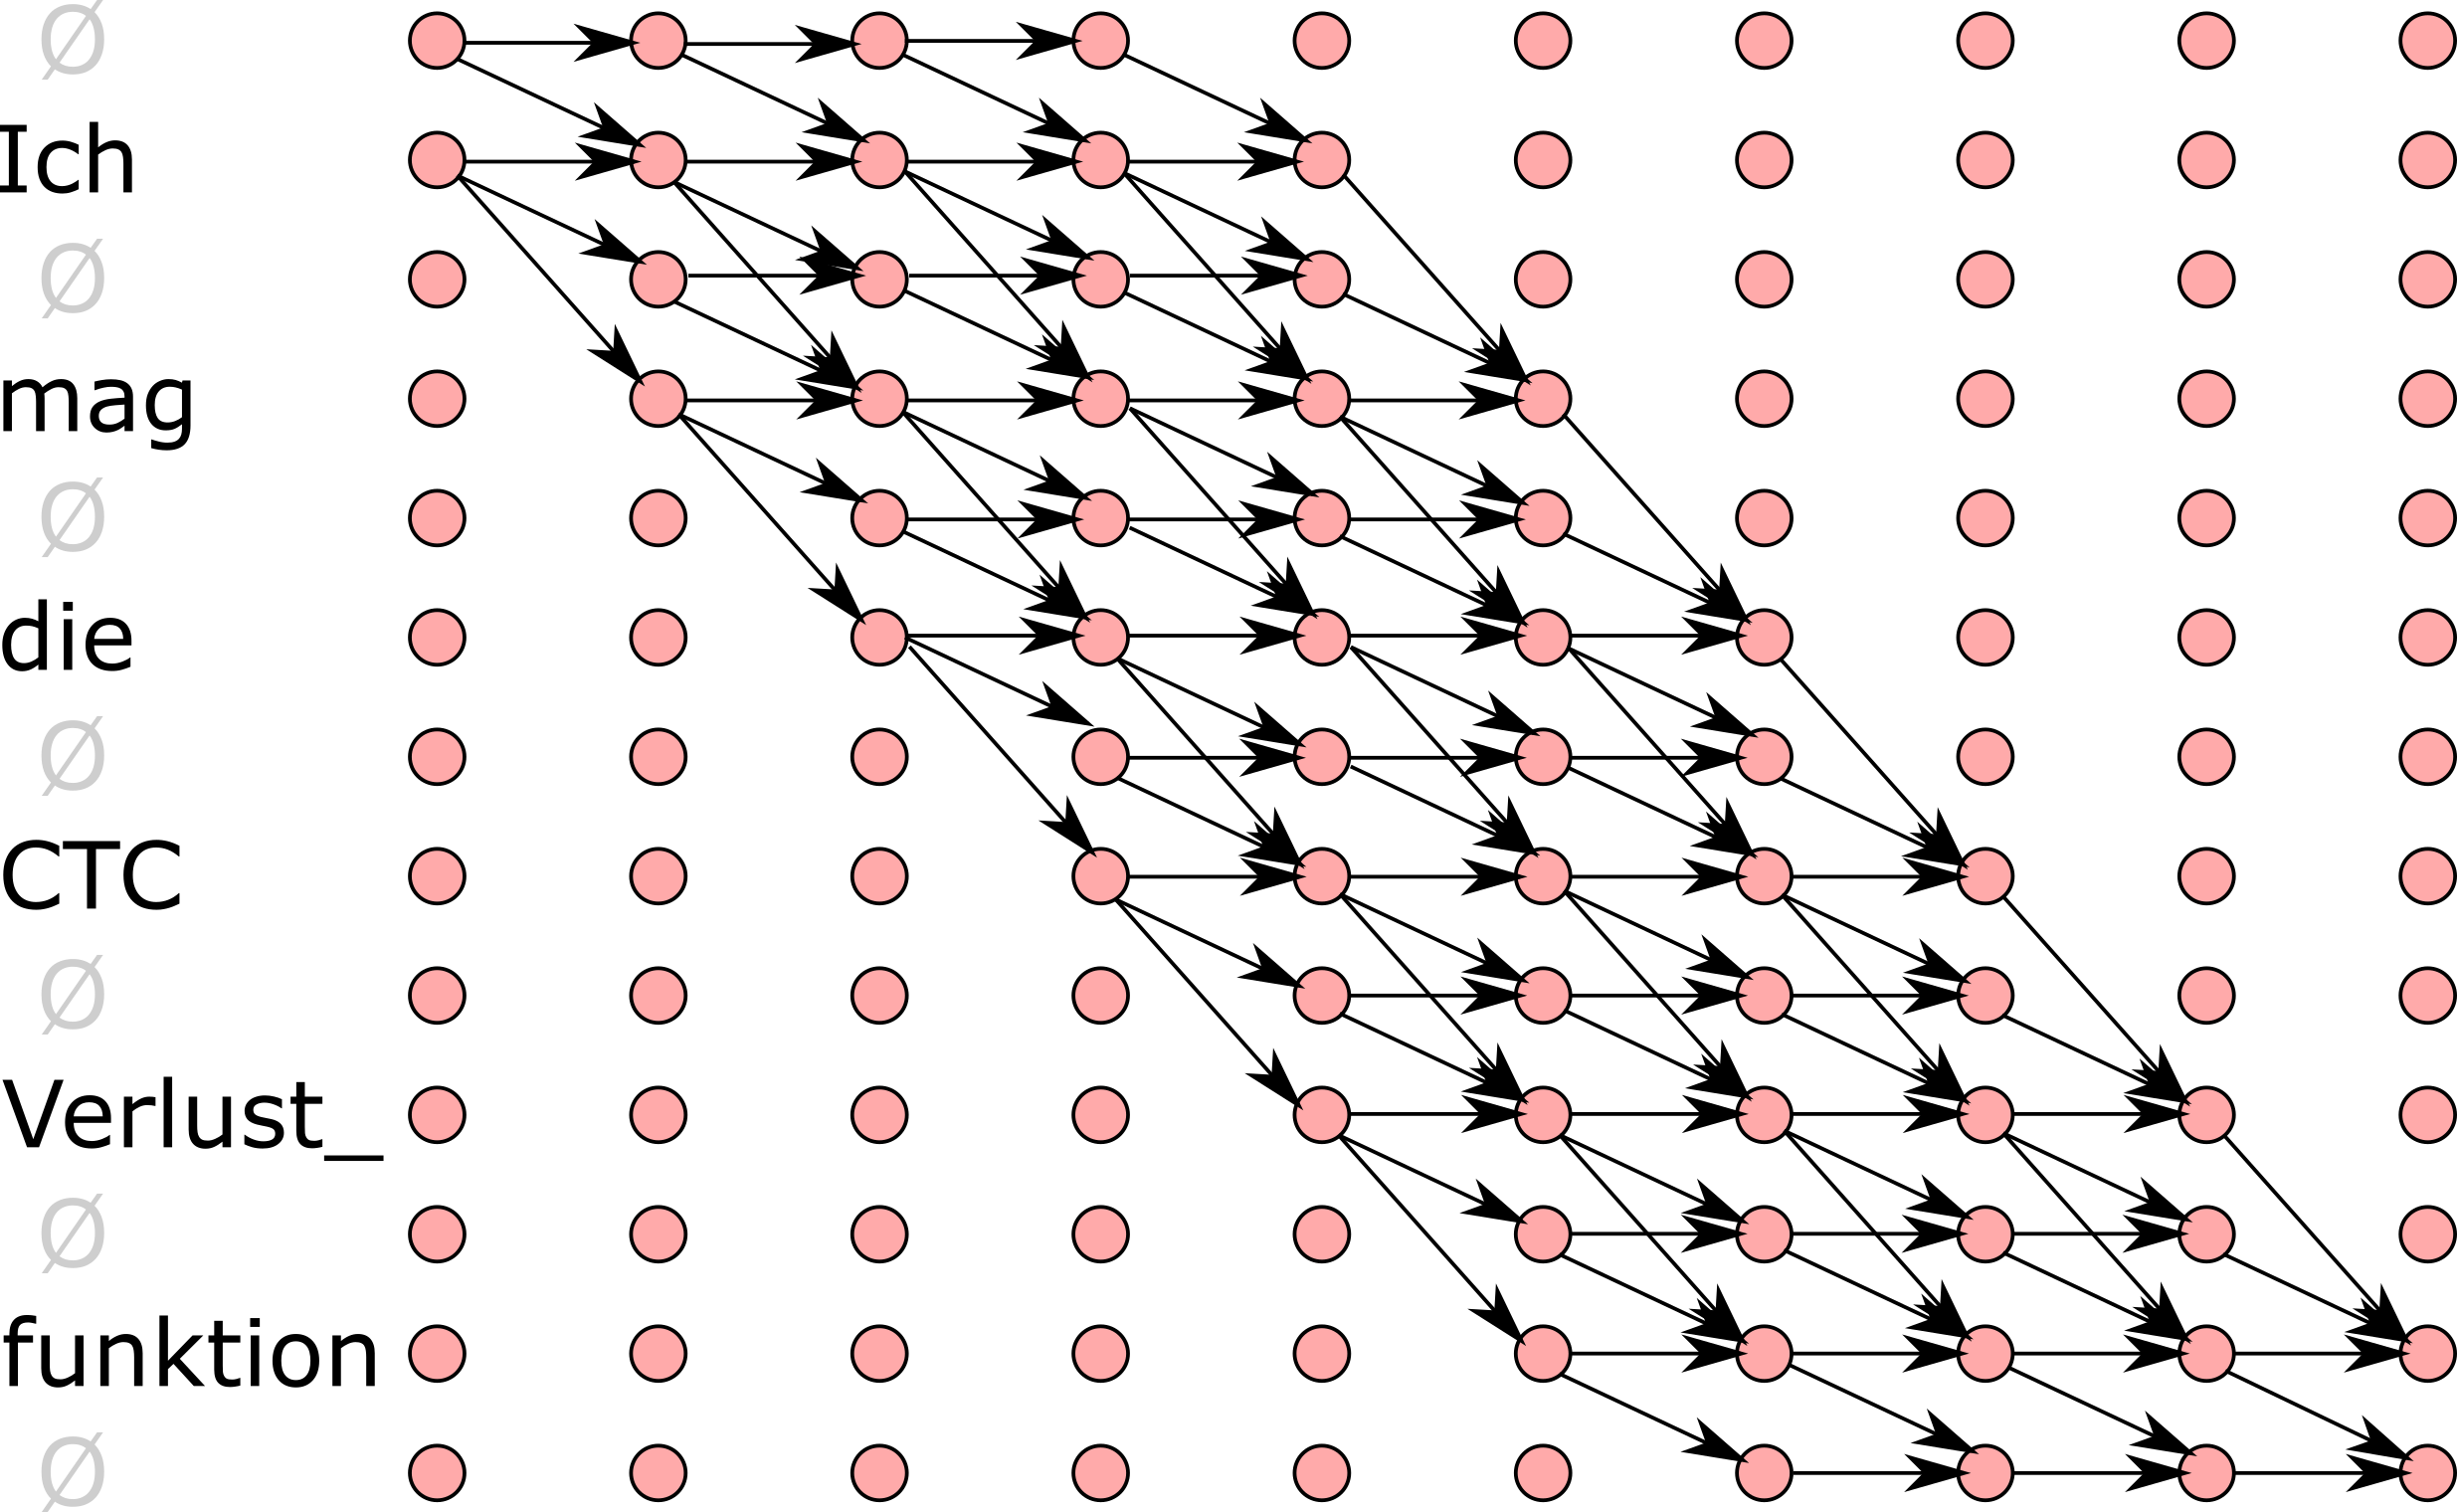
\includegraphics[width=13cm]{img/ctc_schema.png}

  \caption{An illustration of the algorihm for the CTC loss computation. Each
    node denotes producing either a token from the label sequence, or the blank
    token. Each path from one of the two top-left nodes to one of the two
    bottom-right nodes corresponds to one of the equivalent sequences.  }
  \label{fig:ctc-dynamic-programming}
\end{figure}

The \ac{ctc} loss computation is illustrated in Figure
\ref{fig:ctc-dynamic-programming}. The rows represent tokens from the label
sequence plus the optional blank tokens. The columns represent the output state
sequence.  Each node in the graph denotes generating a label from an output
state. The arrows show valid transitions between the generation steps. An arrow
can only go down one or two rows, or horizontally.  The horizontal arrows
denote repeated generation of the same label. These labels are later merged to
form a single output. An arrow can only go two rows down when the skipped row
corresponds to the blank token, so no target tokens are left out. Each path in
the diagram therefore shows one of the equivalent sequences that lead to
generating the given label sequence.

Using the idea that many of the paths from left to right in the diagram share
segments, we can apply dynamic programming to compute the sum of losses across
all paths without the need to enumerate each of them. A node on coordinates
$(i,j)$ stores the accumulated losses for the all path prefixes that lead to
the node, added with the negative log likelihood of the label on the $i$-th row
being generated by the $j$-th output state. The two bottom-right nodes then
store the sum of losses of all the paths.


\JH{doplnit} The training of the network with \ac{ctc} is done by minimizing
the \ac{ctc} loss function, which is defined as follows.

% -----------------------------------------------------------------------------
\section{Model Architecture}
\label{sec:ctc:arch}
% -----------------------------------------------------------------------------

As said in the previous chapter, training models with \ac{ctc} does not impose
any requirements on the model architecture. In our experiments, we aim for a
reasonable comparison between our proposed approach and the state-of-the-art
autoregressive models. We adapt the Transformer model and use similar
hyperparameters where applicable.

Non-autoregressive models generate the outputs in parallel, which requires that
the output length is known beforehand. In autoregressive models, the end of
sequence is indicated by a special end symbol, and the constraint on maximum
length is merely a technical aspect.

To leverage the ability to output empty tokens to the full extent, the output
length should be set to a higher number than the length of the target sequence.
Since the length estimation does not need to be accurate, we select a number
$k$ and we set the target sequence length to be $k$ times longer than the
source length. Note that in case the selected length is shorter than the label
sequence, the model will not be able to generate the whole target sequence.

\begin{figure}
  \centering
  \def\inputsize{7}

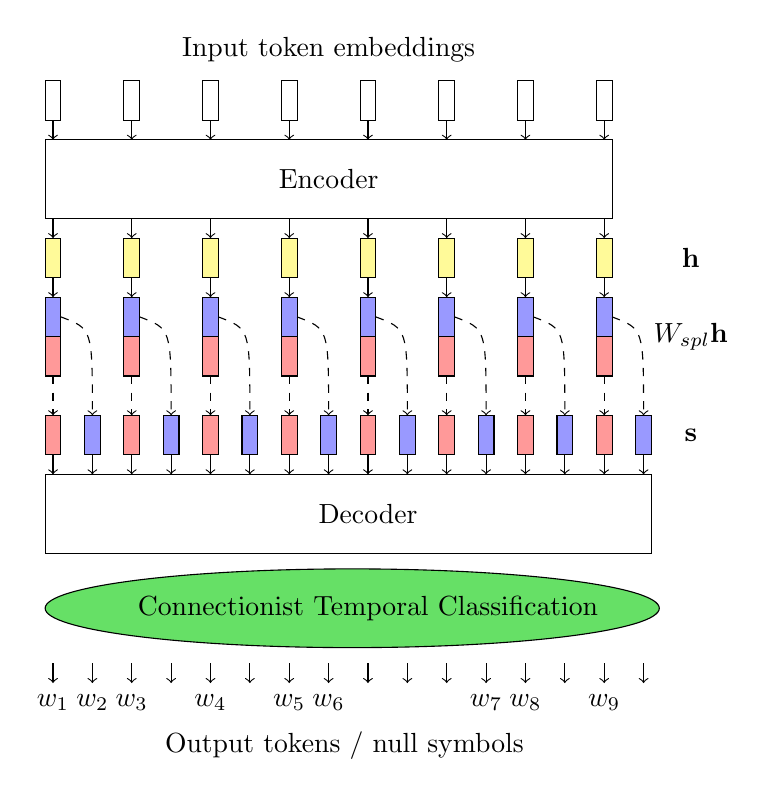
\begin{tikzpicture}[]

\draw (\inputsize / 2 + 0.1, -0.1) node {Input token embeddings};

\foreach \i in {0,...,\inputsize} {
	\draw (\i,-0.5) rectangle (\i+0.2,-1);
    \draw [->] (\i+0.1,-1) -- (\i+0.1, -1.25);
};

\draw (0, -1.25) rectangle (\inputsize + 0.2, -2.25);
\draw (\inputsize / 2 + 0.1, -1.75) node {Encoder};

\foreach \i in {0,...,\inputsize} {
	\draw [->] (\i+0.1,-2.25) -- (\i+0.1, -2.5);
    \draw[fill=yellow!40] (\i,-2.5) rectangle (\i+0.2,-3);

    \draw [->] (\i+0.1,-3) -- (\i+0.1, -3.25);
	\draw[fill=blue!40] (\i,-3.25) rectangle (\i+0.2,-3.75);
	\draw[fill=red!40] (\i,-3.75) rectangle (\i+0.2,-4.25);

    \draw [dashed,->] (\i+0.1,-4.25) -  - (\i+0.1, -4.75);
    \draw [dashed,->] (\i+0.2,-3.5) .. controls (\i + 0.6, -3.65) .. (\i+0.6, -4.75);

	\draw[fill=red!40] (\i,-4.75) rectangle (\i+0.2,-5.25);
	\draw[fill=blue!40] (\i + 0.5,-4.75) rectangle (\i+0.7,-5.25);

    \draw [->] (\i+0.1,-5.25) - - (\i+0.1, -5.5);
    \draw [->] (\i+0.6,-5.25) - - (\i+0.6, -5.5);
};

\draw (\inputsize + 1.2, -2.75) node {$\mathbf{h}$};
\draw (\inputsize + 1.2, -3.75) node {$W_{\text{spl}}\mathbf{h}$};
\draw (\inputsize + 1.2, -5.00) node {$\mathbf{s}$};

\draw (0, -5.5) rectangle (\inputsize + 0.7, -6.5);
\draw (\inputsize / 2 + 0.5 + 0.1, -6.0) node {Decoder};

\draw [fill=green!80!black!60] (\inputsize / 2 + 0.4,-7.2) circle [x radius=\inputsize / 2 + 0.4, y radius=0.5];
\draw (\inputsize / 2 + 0.6, -7.2) node {Connectionist Temporal Classification};

\foreach \i in {0,...,\inputsize} {
   \draw [->] (\i+0.1,-7.9) - - (\i+0.1, -8.15);
   \draw [->] (\i+0.6,-7.9) - - (\i+0.6, -8.15);
}

\draw  (0+0.1,-8.4) node {$w_1$};
\draw  (0+0.6,-8.4) node {$w_2$};
\draw  (1+0.1,-8.4) node {$w_3$};
\draw  (1+0.6,-8.4) node {$\varnothing$};
\draw  (2+0.1,-8.4) node {$w_4$};
\draw  (2+0.6,-8.4) node {$\varnothing$};
\draw  (3+0.1,-8.4) node {$w_5$};
\draw  (3+0.6,-8.4) node {$w_6$};
\draw  (4+0.1,-8.4) node {$\varnothing$};
\draw  (4+0.6,-8.4) node {$\varnothing$};
\draw  (5+0.1,-8.4) node {$\varnothing$};
\draw  (5+0.6,-8.4) node {$w_7$};
\draw  (6+0.1,-8.4) node {$w_8$};
\draw  (6+0.6,-8.4) node {$\varnothing$};
\draw  (7+0.1,-8.4) node {$w_9$};
\draw  (7+0.6,-8.4) node {$\varnothing$};

\draw (\inputsize / 2 + 0.3, -8.95) node {Output tokens / null symbols};

\end{tikzpicture}

  \caption{The scheme of the non-autoregressive architecture with
    state-splitting and CTC. The image is taken from
    \citet{libovicky-helcl-2018-end}.}%
  \label{fig:state-splitting}
\end{figure}


We implement the source-to-target length expansion by linear projections and
state splitting. This mechanism is illustrated in Figure
\ref{fig:state-splitting}. After a given Transformer layer completes its
computation, we linearly project the states
$h_1, \ldots, h_{T_x} \in \mathbb{R}^d$ into $\mathbb{R}^{kd}$. Then, we split
each of these projections into $k$ parts, which results to a $k$-times longer
sequence of states $s_1, \ldots, s_{k \cdot T_x}$ of the original dimension
$d$:
%
\begin{equation}
  s_{ck+b} = \left( W_{\text{spl}} h_c + b_{\text{spl}} \right)_{bd:(b+1)d}
\end{equation}
%
for $b=0 \ldots k-1$ and $c=1 \ldots T_x$ where
$W_{\text{spl}} \in \mathbb{R}^{d \times kd}$ and
$b_{\text{spl}} \in \mathbb{R}^{kd}$ are the trainable projection parameters.

We experiment with two placement options of the state splitting layer. First,
we try placing the state splitting at the end of the Transformer layer
stack. In this scenario, there are 12 Transformer encoder layers, followed by
the state splitting layer, whose outputs are used in the output
projection. Second, we place the state splitting layer in the middle of the
Transformer layer stack, mimicking the 6-layer encoder-decoder architecture of
the autoregressive Transformer model. In the second variant, cross-attention
can be included in the second half of the layers, which attends to the states
right after state splitting.

% -----------------------------------------------------------------------------
\section{Preliminary Experiments}%
\label{sec:ctc:experiments}
% -----------------------------------------------------------------------------

\JH{Section with experiments from the 2018 paper. Should show that it works,
  but it's still far from perfect.}

We conduct experiments with \ac{ctc}-based \ac{nat} models trained on
English--German and English--Romanian translation in both directions.

\paragraph{Data.}
In our experiments, we use the parallel data provided by the \acs{wmt}
organizers. For English--German, the training data consist of the Europarl
corpus \citep{koehn-2005-europarl}, News commentary
\citep{tiedemann-2012-parallel}, and Common
Crawl.\footnote{\url{https://commoncrawl.org/}} For validation, we use the
WMT~13 test set \citep{bojar-etal-2013-findings}, and we evaluate the
translation quality on the WMT~14 test set
\citep{bojar-etal-2014-findings}. For English--Romanian, the data consist of
the Europarl corpus, and the SETIMES corpus distributed by OPUS
\citep{tiedemann-2012-parallel}. We use the development and test set from
WMT~16 \citep{bojar-etal-2016-findings}. The data sizes are shown in
Table~\ref{tab:end-to-end:data}.

\begin{table}
  \centering
  \begin{tabular}{lr}
    \toprule
     & Sentence pairs \\
    \midrule
    En -- De & 4.58 M \\
    En -- Ro & 613 k \\
    \bottomrule
  \end{tabular}

  \caption{The training data sizes. \JH{more}}%
  \label{tab:end-to-end:data}
\end{table}

We preprocess the data with scripts from the \texttt{mosesdecoder}
repository,\footnote{\url{https://github.com/moses-smt/mosesdecoder/}} a part
of the Moses translation toolkit \citep{koehn-etal-2007-moses}. Namely, we
normalize the punctuation in the data, then we use the tokenizer and a
truecaser. We segment the data using the wordpiece algorithm, creating a
vocabulary of 32,000 tokens \citep{wu2016google}.

\paragraph{Models and Training.}
We implement and train our models in the Neural Monkey toolkit
\citep{helcl-libovicky-2017-neural,helcl-etal-2018-neural}. Neural Monkey is a
higher-level deep learning toolkit implemented in TensorFlow
\citep{tensorflow2015-whitepaper}, aiming for fast prototyping using
simple-format configuration files. We train all models for 10 epochs and we
select the best-scoring model based on the validation BLEU score. The training
of the En--De models on a single Nvidia GeForce GTX 1080 GPU took approximately
4 weeks. Since the En--Ro parallel data was much smaller, the training of the
En--Ro models took 4 days.

We summarize the model and training settings in Table
\ref{tab:end-to-end:hparams}. Note that the architecture resembles the
Transformer big settigns, but uses a smaller model dimension. We use the same
settings for training models in both directions in both language pairs.

\begin{table}
  \centering
  \begin{tabular}{lr}
    \toprule
    Parameter & Value \\
    \midrule
    No. of encoder layers & 6 \\
    No. of decoder layers & 6 \\
    Model dimension & 512 \\
    Attention heads & 16 \\
    Dropout probability & 0.1 \\
    Feed-forward hidden size & 4,096 \\
    State splitting factor & 3 \\
    State splitting projection size & 1,536 \\
    Vocabulary size & 32,000 \\
    \midrule
    Optimizer method & adam \\
    $\beta_1$ & 0.9 \\
    $\beta_2$ & 0.997 \\
    $\epsilon$ & 10\textsuperscript{-9} \\
    Learning rate & 10\textsuperscript{-4} \\
    Fixed batch size & 20 \\
    Gradient clipping & 1 \\
    \bottomrule
  \end{tabular}

  \caption{Experimental settings for the Neural Monkey experiments.}%
  \label{tab:end-to-end:hparams}
\end{table}

\paragraph{Results.} Table \ref{tab:end-to-end:bleu} compares the quantitative
results of our non-autoregressive models with methods proposed by
\citet{gu2017nonautoregressive} and \citet{lee-etal-2018-deterministic}. We use
the SacreBLEU \citep{post-2018-call} to compute the BLEU scores of the model
outputs.

\begin{table}
  \centering
  \begin{tabular}{lcccc}
    \toprule
     & \multicolumn{2}{c}{WMT~16} & \multicolumn{2}{c}{WMT~14} \\
     & En $\rightarrow$ Ro & Ro $\rightarrow$ En & En $\rightarrow$ De & De $\rightarrow$ En \\
    \midrule
    \citet{gu2017nonautoregressive} & & & & \\
    Autoregressive baseline & 31.35 & 31.03 & 22.71 & 26.39 \\
    \addlinespace
    NAT + FT & 27.29 & 29.06 & 17.69 & 21.47 \\
    NAT + FT + NPD (100 s) & 29.79 & 31.44 & 19.17 & 23.20 \\
    \midrule
    \citet{lee-etal-2018-deterministic} & & & & \\
    Autoregressive baseline & 31.93 & 31.55  & 23.77 & 28.15 \\
    \addlinespace
    1 iteration & 24.45 & 25.73 & 13.91 & 16.77 \\
    10 iterations & 29.32 & 30.19 & 21.61 & 25.48 \\
    \midrule
    \citet{libovicky-helcl-2018-end} & & & & \\
    Autoregressive baseline & 21.19 & 29.64 & 22.94 & 28.58 \\
    \addlinespace
    Deep encoder & 17.33 & 22.85 & 12.21 & 12.53 \\
    \quad + weight averaging & 18.47 & 24.68 & 14.65 & 16.72 \\
    \quad + beam search & 18.70 & 25.28 & 15.19 & 17.58 \\
    \addlinespace
    Encoder-decoder  & 18.51 & 22.37 & 13.29 & 17.98 \\
    \quad + weight averaging & 19.54 & 24.67 & 16.56 & 18.64 \\
    \quad + beam search & 19.81 & 25.21 & 17.09 & 18.80  \\
    \addlinespace
    Encoder-decoder with pos. enc. & 18.13 & 22.75 & 12.51 & 11.35 \\
    \quad + weight averaging & 19.31 & 24.21 & 17.37 & 18.07 \\
    \quad + beam search & 19.93 & 24.71 & 17.68 & 19.80 \\
    \bottomrule
  \end{tabular}

  \caption{Automatic evaluation of our \acs{ctc}-based approach, compared to
    the two of the first non-autoregressive methods, along with autoregressive
    greedy-decoding baseline scores. }%
  \label{tab:end-to-end:bleu}
\end{table}

The first model of \citet{gu2017nonautoregressive} represents the \ac{nat}
model with fine-tuning, which minimizes the KL divergence between the output
distributions of the teacher and student models. In the second row, \ac{npd}
with 100 samples is used. \JH{This should be described in Related work.} Using
\ac{npd} can slow down the decoding, because an additional scoring step by an
autoregressive model is needed. In theory, if enough parallelism is available,
this doubles the latency.

The approach of \citet{lee-etal-2018-deterministic} is iterative. We show the
performance of this method with 1 iteration and with 10 iterations. Note that
using more iterations slows down the decoding speed of the iterative model.

When compared to the single-pass models, the performance of the English--German
\acs{ctc}-based models is similar. However, the performance of the
English--Romanian models is poor. This is likely because of issues with
Romanian diacritics in the data, as suggested also by the poorer performance of
our autoregressive baseline. Also, the enhanced techniques (\ac{npd} and
iterative refiniment) outperform our method in all scenarios, but at a
computational cost.

The decoding speed for \ac{ar} and {nar} models under different conditions is
shown in Table~\ref{tab:end-to-end:speed}. We report the average time to decode
a single sentence on the \ac{wmt}~15 test set \citep{bojar-etal-2015-findings},
which consists of 2,169 sentence pairs. In the CPU setting, we are using a CPU
machine with the TensorFlow session configured to use 12 CPU threads. The GPU
results are measured on a single Nvidia GeForce GTX 1080 GPU. We show the
average latency as well as the average time to decode a sentence when using
batch decoding.
\JH{Compare speed results? Or leave it for the next chapter.}

\begin{table}
  \centering

  \begin{tabular}{lrr}
    \toprule
     & \mc{CPU} & \mc{GPU} \\
    \midrule
    \acs{ar}, batch=1 & 2,247 ms & 1,129 ms \\
    \acs{ar}, batch=100 & & 127 ms\\
    % AR, beam=?
    \addlinespace
    \acs{nar}, batch=1 & 397 ms & 353 ms  \\
    \acs{nar}, batch=100 &  & 41 ms \\
    \bottomrule
  \end{tabular}

  \caption{The average times to decode one sentence under different conditions.}%
  \label{tab:end-to-end:speed}

\end{table}

Figure \ref{fig:end-to-end:speed} shows the decoding latencies on sentences
from the \ac{wmt}~15 test set \citep{bojar-etal-2015-findings}. As we can see
from the relationship between the source sentence length and the decoding time,
the non-autoregressive model exhibits lower time complexity than the
autoregressive model. The latencies in the plot were measured on a CPU server
using 12 threads. We used greedy decoding with a single sentence in a batch.

\begin{figure}
  \centering
  \begin{tikzpicture}[gnuplot]
%% generated with GNUPLOT 5.2p8 (Lua 5.3; terminal rev. Nov 2018, script rev. 108)
%% Tue 12 Oct 2021 04:15:30 PM BST
\path (0.000,0.000) rectangle (9.000,7.000);
\gpcolor{color=gp lt color border}
\gpsetlinetype{gp lt border}
\gpsetdashtype{gp dt solid}
\gpsetlinewidth{1.00}
\draw[gp path] (0.920,0.986)--(1.100,0.986);
\draw[gp path] (8.815,0.986)--(8.635,0.986);
\node[gp node right] at (0.736,0.986) {$0$};
\draw[gp path] (0.920,1.988)--(1.100,1.988);
\draw[gp path] (8.815,1.988)--(8.635,1.988);
\node[gp node right] at (0.736,1.988) {$1$};
\draw[gp path] (0.920,2.990)--(1.100,2.990);
\draw[gp path] (8.815,2.990)--(8.635,2.990);
\node[gp node right] at (0.736,2.990) {$2$};
\draw[gp path] (0.920,3.993)--(1.100,3.993);
\draw[gp path] (8.815,3.993)--(8.635,3.993);
\node[gp node right] at (0.736,3.993) {$3$};
\draw[gp path] (0.920,4.995)--(1.100,4.995);
\draw[gp path] (8.815,4.995)--(8.635,4.995);
\node[gp node right] at (0.736,4.995) {$4$};
\draw[gp path] (0.920,5.997)--(1.100,5.997);
\draw[gp path] (8.815,5.997)--(8.635,5.997);
\node[gp node right] at (0.736,5.997) {$5$};
\draw[gp path] (0.920,6.999)--(1.100,6.999);
\draw[gp path] (8.815,6.999)--(8.635,6.999);
\node[gp node right] at (0.736,6.999) {$6$};
\draw[gp path] (0.920,0.986)--(0.920,1.166);
\draw[gp path] (0.920,6.999)--(0.920,6.819);
\node[gp node center] at (0.920,0.678) {$0$};
\draw[gp path] (2.499,0.986)--(2.499,1.166);
\draw[gp path] (2.499,6.999)--(2.499,6.819);
\node[gp node center] at (2.499,0.678) {$20$};
\draw[gp path] (4.078,0.986)--(4.078,1.166);
\draw[gp path] (4.078,6.999)--(4.078,6.819);
\node[gp node center] at (4.078,0.678) {$40$};
\draw[gp path] (5.657,0.986)--(5.657,1.166);
\draw[gp path] (5.657,6.999)--(5.657,6.819);
\node[gp node center] at (5.657,0.678) {$60$};
\draw[gp path] (7.236,0.986)--(7.236,1.166);
\draw[gp path] (7.236,6.999)--(7.236,6.819);
\node[gp node center] at (7.236,0.678) {$80$};
\draw[gp path] (8.815,0.986)--(8.815,1.166);
\draw[gp path] (8.815,6.999)--(8.815,6.819);
\node[gp node center] at (8.815,0.678) {$100$};
\draw[gp path] (0.920,6.999)--(0.920,0.986)--(8.815,0.986)--(8.815,6.999)--cycle;
\node[gp node center,rotate=-270] at (-0.016,3.992) {decoding time in seconds};
\node[gp node center] at (4.867,0.216) {source subwords};
\gpcolor{rgb color={0.800,0.000,0.000}}
\gpsetlinewidth{5.50}
\draw[gp path] (0.920,1.263)--(1.000,1.336)--(1.079,1.410)--(1.159,1.484)--(1.239,1.558)%
  --(1.319,1.632)--(1.398,1.706)--(1.478,1.780)--(1.558,1.853)--(1.638,1.927)--(1.717,2.001)%
  --(1.797,2.075)--(1.877,2.149)--(1.957,2.223)--(2.036,2.297)--(2.116,2.371)--(2.196,2.444)%
  --(2.276,2.518)--(2.355,2.592)--(2.435,2.666)--(2.515,2.740)--(2.595,2.814)--(2.674,2.888)%
  --(2.754,2.961)--(2.834,3.035)--(2.914,3.109)--(2.993,3.183)--(3.073,3.257)--(3.153,3.331)%
  --(3.233,3.405)--(3.312,3.478)--(3.392,3.552)--(3.472,3.626)--(3.552,3.700)--(3.631,3.774)%
  --(3.711,3.848)--(3.791,3.922)--(3.871,3.996)--(3.950,4.069)--(4.030,4.143)--(4.110,4.217)%
  --(4.190,4.291)--(4.269,4.365)--(4.349,4.439)--(4.429,4.513)--(4.509,4.586)--(4.588,4.660)%
  --(4.668,4.734)--(4.748,4.808)--(4.828,4.882)--(4.907,4.956)--(4.987,5.030)--(5.067,5.103)%
  --(5.147,5.177)--(5.226,5.251)--(5.306,5.325)--(5.386,5.399)--(5.466,5.473)--(5.545,5.547)%
  --(5.625,5.621)--(5.705,5.694)--(5.785,5.768)--(5.864,5.842)--(5.944,5.916)--(6.024,5.990)%
  --(6.104,6.064)--(6.183,6.138)--(6.263,6.211)--(6.343,6.285)--(6.423,6.359)--(6.502,6.433)%
  --(6.582,6.507)--(6.662,6.581)--(6.742,6.655)--(6.821,6.729)--(6.901,6.802)--(6.981,6.876)%
  --(7.061,6.950)--(7.113,6.999);
\gpcolor{rgb color={0.000,0.000,0.800}}
\draw[gp path] (0.920,1.215)--(1.000,1.221)--(1.079,1.227)--(1.159,1.233)--(1.239,1.239)%
  --(1.319,1.244)--(1.398,1.250)--(1.478,1.256)--(1.558,1.262)--(1.638,1.268)--(1.717,1.274)%
  --(1.797,1.280)--(1.877,1.286)--(1.957,1.292)--(2.036,1.298)--(2.116,1.304)--(2.196,1.310)%
  --(2.276,1.316)--(2.355,1.322)--(2.435,1.328)--(2.515,1.333)--(2.595,1.339)--(2.674,1.345)%
  --(2.754,1.351)--(2.834,1.357)--(2.914,1.363)--(2.993,1.369)--(3.073,1.375)--(3.153,1.381)%
  --(3.233,1.387)--(3.312,1.393)--(3.392,1.399)--(3.472,1.405)--(3.552,1.411)--(3.631,1.417)%
  --(3.711,1.422)--(3.791,1.428)--(3.871,1.434)--(3.950,1.440)--(4.030,1.446)--(4.110,1.452)%
  --(4.190,1.458)--(4.269,1.464)--(4.349,1.470)--(4.429,1.476)--(4.509,1.482)--(4.588,1.488)%
  --(4.668,1.494)--(4.748,1.500)--(4.828,1.506)--(4.907,1.511)--(4.987,1.517)--(5.067,1.523)%
  --(5.147,1.529)--(5.226,1.535)--(5.306,1.541)--(5.386,1.547)--(5.466,1.553)--(5.545,1.559)%
  --(5.625,1.565)--(5.705,1.571)--(5.785,1.577)--(5.864,1.583)--(5.944,1.589)--(6.024,1.594)%
  --(6.104,1.600)--(6.183,1.606)--(6.263,1.612)--(6.343,1.618)--(6.423,1.624)--(6.502,1.630)%
  --(6.582,1.636)--(6.662,1.642)--(6.742,1.648)--(6.821,1.654)--(6.901,1.660)--(6.981,1.666)%
  --(7.061,1.672)--(7.140,1.678)--(7.220,1.683)--(7.300,1.689)--(7.380,1.695)--(7.459,1.701)%
  --(7.539,1.707)--(7.619,1.713)--(7.699,1.719)--(7.778,1.725)--(7.858,1.731)--(7.938,1.737)%
  --(8.018,1.743)--(8.097,1.749)--(8.177,1.755)--(8.257,1.761)--(8.337,1.767)--(8.416,1.772)%
  --(8.496,1.778)--(8.576,1.784)--(8.656,1.790)--(8.735,1.796)--(8.815,1.802);
\gpcolor{color=gp lt color border}
\node[gp node right] at (8.083,4.146) {AR};
\gpcolor{rgb color={0.867,0.000,0.000}}
\gpsetlinewidth{0.80}
\gpsetpointsize{4.00}
\gppoint{gp mark 3}{(1.552,2.944)}
\gppoint{gp mark 3}{(5.104,5.179)}
\gppoint{gp mark 3}{(3.131,3.343)}
\gppoint{gp mark 3}{(2.183,2.426)}
\gppoint{gp mark 3}{(2.262,2.860)}
\gppoint{gp mark 3}{(2.736,2.862)}
\gppoint{gp mark 3}{(4.078,4.814)}
\gppoint{gp mark 3}{(4.473,5.662)}
\gppoint{gp mark 3}{(3.446,3.635)}
\gppoint{gp mark 3}{(3.367,3.611)}
\gppoint{gp mark 3}{(3.131,3.330)}
\gppoint{gp mark 3}{(2.262,2.376)}
\gppoint{gp mark 3}{(2.025,2.338)}
\gppoint{gp mark 3}{(2.104,2.468)}
\gppoint{gp mark 3}{(2.104,2.427)}
\gppoint{gp mark 3}{(2.499,2.610)}
\gppoint{gp mark 3}{(3.525,3.064)}
\gppoint{gp mark 3}{(3.289,3.378)}
\gppoint{gp mark 3}{(3.210,3.444)}
\gppoint{gp mark 3}{(2.341,2.666)}
\gppoint{gp mark 3}{(2.183,2.268)}
\gppoint{gp mark 3}{(2.736,3.253)}
\gppoint{gp mark 3}{(4.710,6.120)}
\gppoint{gp mark 3}{(3.525,3.045)}
\gppoint{gp mark 3}{(3.841,4.057)}
\gppoint{gp mark 3}{(4.473,5.371)}
\gppoint{gp mark 3}{(2.104,2.466)}
\gppoint{gp mark 3}{(3.762,3.850)}
\gppoint{gp mark 3}{(4.315,5.573)}
\gppoint{gp mark 3}{(4.078,4.322)}
\gppoint{gp mark 3}{(5.183,5.537)}
\gppoint{gp mark 3}{(4.631,5.557)}
\gppoint{gp mark 3}{(5.025,5.763)}
\gppoint{gp mark 3}{(5.420,6.596)}
\gppoint{gp mark 3}{(3.052,3.635)}
\gppoint{gp mark 3}{(7.157,6.654)}
\gppoint{gp mark 3}{(2.183,2.611)}
\gppoint{gp mark 3}{(5.183,5.542)}
\gppoint{gp mark 3}{(4.552,5.229)}
\gppoint{gp mark 3}{(2.341,2.600)}
\gppoint{gp mark 3}{(1.394,1.760)}
\gppoint{gp mark 3}{(2.499,2.632)}
\gppoint{gp mark 3}{(3.446,3.726)}
\gppoint{gp mark 3}{(2.183,2.684)}
\gppoint{gp mark 3}{(1.552,1.850)}
\gppoint{gp mark 3}{(3.289,3.640)}
\gppoint{gp mark 3}{(2.973,3.125)}
\gppoint{gp mark 3}{(2.025,2.745)}
\gppoint{gp mark 3}{(3.604,4.848)}
\gppoint{gp mark 3}{(4.946,6.315)}
\gppoint{gp mark 3}{(3.210,3.118)}
\gppoint{gp mark 3}{(3.762,4.093)}
\gppoint{gp mark 3}{(2.578,2.908)}
\gppoint{gp mark 3}{(3.446,4.833)}
\gppoint{gp mark 3}{(6.999,6.565)}
\gppoint{gp mark 3}{(3.604,3.556)}
\gppoint{gp mark 3}{(3.525,3.849)}
\gppoint{gp mark 3}{(3.052,3.918)}
\gppoint{gp mark 3}{(4.078,5.196)}
\gppoint{gp mark 3}{(3.920,3.840)}
\gppoint{gp mark 3}{(2.973,3.290)}
\gppoint{gp mark 3}{(3.683,3.995)}
\gppoint{gp mark 3}{(3.367,4.688)}
\gppoint{gp mark 3}{(2.341,3.394)}
\gppoint{gp mark 3}{(3.052,3.897)}
\gppoint{gp mark 3}{(2.578,3.684)}
\gppoint{gp mark 3}{(3.525,4.390)}
\gppoint{gp mark 3}{(4.710,4.821)}
\gppoint{gp mark 3}{(2.104,2.527)}
\gppoint{gp mark 3}{(2.341,2.127)}
\gppoint{gp mark 3}{(4.157,4.015)}
\gppoint{gp mark 3}{(2.499,2.791)}
\gppoint{gp mark 3}{(3.131,3.106)}
\gppoint{gp mark 3}{(3.999,5.824)}
\gppoint{gp mark 3}{(3.683,4.417)}
\gppoint{gp mark 3}{(5.657,6.625)}
\gppoint{gp mark 3}{(3.920,4.043)}
\gppoint{gp mark 3}{(3.052,2.649)}
\gppoint{gp mark 3}{(3.525,3.645)}
\gppoint{gp mark 3}{(1.552,2.005)}
\gppoint{gp mark 3}{(6.999,6.345)}
\gppoint{gp mark 3}{(3.289,3.319)}
\gppoint{gp mark 3}{(5.104,6.225)}
\gppoint{gp mark 3}{(3.762,3.807)}
\gppoint{gp mark 3}{(3.210,3.795)}
\gppoint{gp mark 3}{(4.710,5.241)}
\gppoint{gp mark 3}{(5.025,5.915)}
\gppoint{gp mark 3}{(2.894,3.333)}
\gppoint{gp mark 3}{(3.367,3.564)}
\gppoint{gp mark 3}{(3.131,3.156)}
\gppoint{gp mark 3}{(3.210,3.442)}
\gppoint{gp mark 3}{(2.341,2.593)}
\gppoint{gp mark 3}{(2.894,2.737)}
\gppoint{gp mark 3}{(2.578,2.972)}
\gppoint{gp mark 3}{(1.473,1.879)}
\gppoint{gp mark 3}{(2.341,2.355)}
\gppoint{gp mark 3}{(3.052,2.832)}
\gppoint{gp mark 3}{(3.683,4.284)}
\gppoint{gp mark 3}{(2.499,2.711)}
\gppoint{gp mark 3}{(3.367,3.440)}
\gppoint{gp mark 3}{(3.525,3.704)}
\gppoint{gp mark 3}{(1.394,1.684)}
\gppoint{gp mark 3}{(1.867,2.397)}
\gppoint{gp mark 3}{(3.683,3.708)}
\gppoint{gp mark 3}{(3.446,3.659)}
\gppoint{gp mark 3}{(4.868,5.945)}
\gppoint{gp mark 3}{(3.683,4.462)}
\gppoint{gp mark 3}{(3.131,2.981)}
\gppoint{gp mark 3}{(2.104,2.743)}
\gppoint{gp mark 3}{(2.973,3.581)}
\gppoint{gp mark 3}{(3.841,4.105)}
\gppoint{gp mark 3}{(1.946,2.099)}
\gppoint{gp mark 3}{(1.788,1.928)}
\gppoint{gp mark 3}{(3.367,2.711)}
\gppoint{gp mark 3}{(2.025,1.893)}
\gppoint{gp mark 3}{(1.552,1.713)}
\gppoint{gp mark 3}{(1.946,1.975)}
\gppoint{gp mark 3}{(2.815,2.784)}
\gppoint{gp mark 3}{(3.052,3.539)}
\gppoint{gp mark 3}{(1.552,1.757)}
\gppoint{gp mark 3}{(4.157,4.178)}
\gppoint{gp mark 3}{(4.236,5.400)}
\gppoint{gp mark 3}{(5.025,5.146)}
\gppoint{gp mark 3}{(5.025,5.332)}
\gppoint{gp mark 3}{(3.525,4.143)}
\gppoint{gp mark 3}{(3.289,4.024)}
\gppoint{gp mark 3}{(3.841,3.512)}
\gppoint{gp mark 3}{(2.104,2.071)}
\gppoint{gp mark 3}{(1.394,1.708)}
\gppoint{gp mark 3}{(4.946,5.767)}
\gppoint{gp mark 3}{(4.473,5.009)}
\gppoint{gp mark 3}{(5.341,6.369)}
\gppoint{gp mark 3}{(5.736,6.023)}
\gppoint{gp mark 3}{(2.420,3.003)}
\gppoint{gp mark 3}{(3.210,2.205)}
\gppoint{gp mark 3}{(3.289,3.305)}
\gppoint{gp mark 3}{(3.920,4.366)}
\gppoint{gp mark 3}{(3.210,3.337)}
\gppoint{gp mark 3}{(3.052,3.570)}
\gppoint{gp mark 3}{(4.078,4.673)}
\gppoint{gp mark 3}{(2.736,2.428)}
\gppoint{gp mark 3}{(2.973,3.309)}
\gppoint{gp mark 3}{(3.604,3.451)}
\gppoint{gp mark 3}{(2.736,3.101)}
\gppoint{gp mark 3}{(1.946,2.072)}
\gppoint{gp mark 3}{(4.789,5.801)}
\gppoint{gp mark 3}{(4.315,4.257)}
\gppoint{gp mark 3}{(4.157,4.017)}
\gppoint{gp mark 3}{(2.104,2.221)}
\gppoint{gp mark 3}{(4.157,3.982)}
\gppoint{gp mark 3}{(4.078,3.748)}
\gppoint{gp mark 3}{(1.315,1.661)}
\gppoint{gp mark 3}{(3.604,3.847)}
\gppoint{gp mark 3}{(7.552,6.636)}
\gppoint{gp mark 3}{(1.236,1.564)}
\gppoint{gp mark 3}{(2.262,2.336)}
\gppoint{gp mark 3}{(3.131,2.492)}
\gppoint{gp mark 3}{(5.578,4.543)}
\gppoint{gp mark 3}{(3.762,3.266)}
\gppoint{gp mark 3}{(2.815,2.305)}
\gppoint{gp mark 3}{(4.946,5.147)}
\gppoint{gp mark 3}{(1.078,1.511)}
\gppoint{gp mark 3}{(3.210,3.651)}
\gppoint{gp mark 3}{(3.131,3.103)}
\gppoint{gp mark 3}{(1.631,2.152)}
\gppoint{gp mark 3}{(6.210,6.525)}
\gppoint{gp mark 3}{(3.683,3.502)}
\gppoint{gp mark 3}{(5.104,5.203)}
\gppoint{gp mark 3}{(4.157,4.412)}
\gppoint{gp mark 3}{(2.183,2.170)}
\gppoint{gp mark 3}{(4.157,4.219)}
\gppoint{gp mark 3}{(3.131,2.982)}
\gppoint{gp mark 3}{(3.052,3.685)}
\gppoint{gp mark 3}{(4.631,5.922)}
\gppoint{gp mark 3}{(4.552,5.776)}
\gppoint{gp mark 3}{(2.025,2.377)}
\gppoint{gp mark 3}{(2.025,1.886)}
\gppoint{gp mark 3}{(3.131,3.850)}
\gppoint{gp mark 3}{(3.289,3.827)}
\gppoint{gp mark 3}{(2.262,2.231)}
\gppoint{gp mark 3}{(5.657,6.239)}
\gppoint{gp mark 3}{(2.499,2.837)}
\gppoint{gp mark 3}{(2.183,2.276)}
\gppoint{gp mark 3}{(3.841,3.226)}
\gppoint{gp mark 3}{(3.210,3.582)}
\gppoint{gp mark 3}{(2.420,2.730)}
\gppoint{gp mark 3}{(3.210,4.165)}
\gppoint{gp mark 3}{(2.499,2.606)}
\gppoint{gp mark 3}{(3.841,4.587)}
\gppoint{gp mark 3}{(3.210,4.011)}
\gppoint{gp mark 3}{(5.499,5.924)}
\gppoint{gp mark 3}{(3.210,3.835)}
\gppoint{gp mark 3}{(7.315,4.959)}
\gppoint{gp mark 3}{(4.946,4.239)}
\gppoint{gp mark 3}{(4.946,5.662)}
\gppoint{gp mark 3}{(4.078,4.082)}
\gppoint{gp mark 3}{(2.815,3.296)}
\gppoint{gp mark 3}{(4.631,4.627)}
\gppoint{gp mark 3}{(3.525,3.580)}
\gppoint{gp mark 3}{(2.183,2.463)}
\gppoint{gp mark 3}{(1.631,1.818)}
\gppoint{gp mark 3}{(2.025,2.048)}
\gppoint{gp mark 3}{(2.657,2.088)}
\gppoint{gp mark 3}{(3.052,2.864)}
\gppoint{gp mark 3}{(2.499,2.425)}
\gppoint{gp mark 3}{(6.999,6.966)}
\gppoint{gp mark 3}{(2.499,2.818)}
\gppoint{gp mark 3}{(1.867,1.966)}
\gppoint{gp mark 3}{(4.473,4.515)}
\gppoint{gp mark 3}{(1.788,2.192)}
\gppoint{gp mark 3}{(2.894,3.169)}
\gppoint{gp mark 3}{(3.841,4.028)}
\gppoint{gp mark 3}{(3.289,3.483)}
\gppoint{gp mark 3}{(3.999,4.159)}
\gppoint{gp mark 3}{(2.657,2.903)}
\gppoint{gp mark 3}{(3.999,4.427)}
\gppoint{gp mark 3}{(3.131,3.302)}
\gppoint{gp mark 3}{(3.525,3.764)}
\gppoint{gp mark 3}{(4.236,4.758)}
\gppoint{gp mark 3}{(5.262,4.952)}
\gppoint{gp mark 3}{(5.183,5.952)}
\gppoint{gp mark 3}{(1.867,1.981)}
\gppoint{gp mark 3}{(2.815,2.990)}
\gppoint{gp mark 3}{(2.420,2.904)}
\gppoint{gp mark 3}{(3.762,4.119)}
\gppoint{gp mark 3}{(3.289,3.267)}
\gppoint{gp mark 3}{(2.657,2.335)}
\gppoint{gp mark 3}{(3.210,3.205)}
\gppoint{gp mark 3}{(4.315,4.664)}
\gppoint{gp mark 3}{(3.920,3.858)}
\gppoint{gp mark 3}{(1.236,1.626)}
\gppoint{gp mark 3}{(5.578,5.122)}
\gppoint{gp mark 3}{(6.525,5.554)}
\gppoint{gp mark 3}{(3.052,2.977)}
\gppoint{gp mark 3}{(6.131,6.022)}
\gppoint{gp mark 3}{(5.025,5.077)}
\gppoint{gp mark 3}{(2.736,2.482)}
\gppoint{gp mark 3}{(4.631,4.383)}
\gppoint{gp mark 3}{(2.657,2.851)}
\gppoint{gp mark 3}{(3.052,2.935)}
\gppoint{gp mark 3}{(1.631,1.846)}
\gppoint{gp mark 3}{(1.631,2.233)}
\gppoint{gp mark 3}{(1.710,2.295)}
\gppoint{gp mark 3}{(2.025,2.147)}
\gppoint{gp mark 3}{(4.078,4.263)}
\gppoint{gp mark 3}{(2.973,2.352)}
\gppoint{gp mark 3}{(3.920,4.356)}
\gppoint{gp mark 3}{(2.578,2.801)}
\gppoint{gp mark 3}{(6.052,6.778)}
\gppoint{gp mark 3}{(3.683,3.924)}
\gppoint{gp mark 3}{(3.920,3.508)}
\gppoint{gp mark 3}{(5.262,5.262)}
\gppoint{gp mark 3}{(2.815,2.798)}
\gppoint{gp mark 3}{(3.683,4.368)}
\gppoint{gp mark 3}{(1.946,2.098)}
\gppoint{gp mark 3}{(2.499,2.731)}
\gppoint{gp mark 3}{(2.499,2.523)}
\gppoint{gp mark 3}{(2.341,2.252)}
\gppoint{gp mark 3}{(3.604,3.145)}
\gppoint{gp mark 3}{(2.420,2.521)}
\gppoint{gp mark 3}{(4.631,4.419)}
\gppoint{gp mark 3}{(1.788,2.238)}
\gppoint{gp mark 3}{(3.446,3.371)}
\gppoint{gp mark 3}{(2.499,2.504)}
\gppoint{gp mark 3}{(3.210,3.436)}
\gppoint{gp mark 3}{(2.262,2.226)}
\gppoint{gp mark 3}{(4.394,4.599)}
\gppoint{gp mark 3}{(2.104,2.766)}
\gppoint{gp mark 3}{(1.946,2.086)}
\gppoint{gp mark 3}{(2.499,2.609)}
\gppoint{gp mark 3}{(3.131,2.841)}
\gppoint{gp mark 3}{(2.341,2.386)}
\gppoint{gp mark 3}{(2.657,2.579)}
\gppoint{gp mark 3}{(1.631,1.964)}
\gppoint{gp mark 3}{(3.446,3.307)}
\gppoint{gp mark 3}{(3.762,3.128)}
\gppoint{gp mark 3}{(2.815,3.420)}
\gppoint{gp mark 3}{(3.999,3.188)}
\gppoint{gp mark 3}{(3.131,3.060)}
\gppoint{gp mark 3}{(2.894,2.780)}
\gppoint{gp mark 3}{(2.262,2.481)}
\gppoint{gp mark 3}{(2.657,2.952)}
\gppoint{gp mark 3}{(4.473,4.237)}
\gppoint{gp mark 3}{(2.420,2.333)}
\gppoint{gp mark 3}{(3.683,3.326)}
\gppoint{gp mark 3}{(5.025,4.768)}
\gppoint{gp mark 3}{(4.789,4.646)}
\gppoint{gp mark 3}{(2.499,2.709)}
\gppoint{gp mark 3}{(3.604,3.797)}
\gppoint{gp mark 3}{(2.025,2.166)}
\gppoint{gp mark 3}{(3.525,3.882)}
\gppoint{gp mark 3}{(3.367,3.355)}
\gppoint{gp mark 3}{(5.341,6.181)}
\gppoint{gp mark 3}{(1.867,2.201)}
\gppoint{gp mark 3}{(5.420,5.768)}
\gppoint{gp mark 3}{(4.868,4.606)}
\gppoint{gp mark 3}{(4.631,4.492)}
\gppoint{gp mark 3}{(2.736,2.879)}
\gppoint{gp mark 3}{(6.447,6.654)}
\gppoint{gp mark 3}{(6.289,6.428)}
\gppoint{gp mark 3}{(5.104,5.737)}
\gppoint{gp mark 3}{(6.762,4.954)}
\gppoint{gp mark 3}{(2.341,1.977)}
\gppoint{gp mark 3}{(1.946,2.089)}
\gppoint{gp mark 3}{(1.788,2.008)}
\gppoint{gp mark 3}{(2.736,3.223)}
\gppoint{gp mark 3}{(2.499,2.504)}
\gppoint{gp mark 3}{(4.315,4.318)}
\gppoint{gp mark 3}{(2.578,2.675)}
\gppoint{gp mark 3}{(1.946,2.108)}
\gppoint{gp mark 3}{(3.131,2.728)}
\gppoint{gp mark 3}{(1.473,1.723)}
\gppoint{gp mark 3}{(2.578,2.936)}
\gppoint{gp mark 3}{(1.315,1.688)}
\gppoint{gp mark 3}{(1.078,1.569)}
\gppoint{gp mark 3}{(1.631,1.790)}
\gppoint{gp mark 3}{(5.183,5.202)}
\gppoint{gp mark 3}{(1.710,1.912)}
\gppoint{gp mark 3}{(2.657,2.640)}
\gppoint{gp mark 3}{(4.236,4.328)}
\gppoint{gp mark 3}{(4.552,3.600)}
\gppoint{gp mark 3}{(3.920,3.600)}
\gppoint{gp mark 3}{(3.683,3.990)}
\gppoint{gp mark 3}{(2.262,3.120)}
\gppoint{gp mark 3}{(2.736,2.849)}
\gppoint{gp mark 3}{(3.999,3.972)}
\gppoint{gp mark 3}{(3.052,3.200)}
\gppoint{gp mark 3}{(2.104,2.318)}
\gppoint{gp mark 3}{(1.473,1.875)}
\gppoint{gp mark 3}{(1.710,1.771)}
\gppoint{gp mark 3}{(1.315,1.621)}
\gppoint{gp mark 3}{(2.025,1.764)}
\gppoint{gp mark 3}{(1.710,1.724)}
\gppoint{gp mark 3}{(2.657,2.508)}
\gppoint{gp mark 3}{(1.788,1.736)}
\gppoint{gp mark 3}{(2.104,1.834)}
\gppoint{gp mark 3}{(1.788,1.735)}
\gppoint{gp mark 3}{(1.867,2.098)}
\gppoint{gp mark 3}{(1.710,1.873)}
\gppoint{gp mark 3}{(3.683,3.847)}
\gppoint{gp mark 3}{(2.894,3.139)}
\gppoint{gp mark 3}{(1.631,1.621)}
\gppoint{gp mark 3}{(1.710,1.788)}
\gppoint{gp mark 3}{(1.473,1.919)}
\gppoint{gp mark 3}{(3.367,3.142)}
\gppoint{gp mark 3}{(2.736,2.632)}
\gppoint{gp mark 3}{(2.183,2.215)}
\gppoint{gp mark 3}{(3.052,3.064)}
\gppoint{gp mark 3}{(2.025,2.246)}
\gppoint{gp mark 3}{(2.420,2.690)}
\gppoint{gp mark 3}{(4.315,4.222)}
\gppoint{gp mark 3}{(1.473,1.657)}
\gppoint{gp mark 3}{(4.789,5.428)}
\gppoint{gp mark 3}{(1.552,1.832)}
\gppoint{gp mark 3}{(4.631,5.146)}
\gppoint{gp mark 3}{(1.710,1.839)}
\gppoint{gp mark 3}{(2.736,2.206)}
\gppoint{gp mark 3}{(3.289,3.458)}
\gppoint{gp mark 3}{(4.552,4.536)}
\gppoint{gp mark 3}{(3.052,3.433)}
\gppoint{gp mark 3}{(4.157,5.036)}
\gppoint{gp mark 3}{(7.236,6.663)}
\gppoint{gp mark 3}{(2.657,2.704)}
\gppoint{gp mark 3}{(1.552,1.801)}
\gppoint{gp mark 3}{(1.788,2.041)}
\gppoint{gp mark 3}{(4.236,4.192)}
\gppoint{gp mark 3}{(1.710,1.833)}
\gppoint{gp mark 3}{(3.841,4.528)}
\gppoint{gp mark 3}{(3.210,2.418)}
\gppoint{gp mark 3}{(3.052,3.020)}
\gppoint{gp mark 3}{(2.815,2.658)}
\gppoint{gp mark 3}{(1.788,2.108)}
\gppoint{gp mark 3}{(2.341,2.164)}
\gppoint{gp mark 3}{(3.841,3.237)}
\gppoint{gp mark 3}{(2.736,3.041)}
\gppoint{gp mark 3}{(1.394,1.702)}
\gppoint{gp mark 3}{(2.341,2.340)}
\gppoint{gp mark 3}{(1.867,6.019)}
\gppoint{gp mark 3}{(2.815,2.193)}
\gppoint{gp mark 3}{(3.131,3.128)}
\gppoint{gp mark 3}{(2.815,2.975)}
\gppoint{gp mark 3}{(3.999,3.498)}
\gppoint{gp mark 3}{(2.341,2.845)}
\gppoint{gp mark 3}{(2.736,2.888)}
\gppoint{gp mark 3}{(1.710,1.680)}
\gppoint{gp mark 3}{(1.631,2.220)}
\gppoint{gp mark 3}{(2.815,2.445)}
\gppoint{gp mark 3}{(1.788,1.840)}
\gppoint{gp mark 3}{(1.631,2.064)}
\gppoint{gp mark 3}{(2.341,2.356)}
\gppoint{gp mark 3}{(4.236,4.345)}
\gppoint{gp mark 3}{(1.946,1.936)}
\gppoint{gp mark 3}{(1.867,1.728)}
\gppoint{gp mark 3}{(1.788,1.679)}
\gppoint{gp mark 3}{(1.710,1.960)}
\gppoint{gp mark 3}{(4.078,4.109)}
\gppoint{gp mark 3}{(4.078,4.168)}
\gppoint{gp mark 3}{(2.420,2.476)}
\gppoint{gp mark 3}{(3.367,2.806)}
\gppoint{gp mark 3}{(2.499,2.214)}
\gppoint{gp mark 3}{(4.552,4.421)}
\gppoint{gp mark 3}{(1.631,1.837)}
\gppoint{gp mark 3}{(1.236,1.519)}
\gppoint{gp mark 3}{(1.394,1.645)}
\gppoint{gp mark 3}{(1.631,1.617)}
\gppoint{gp mark 3}{(2.736,2.180)}
\gppoint{gp mark 3}{(1.236,1.592)}
\gppoint{gp mark 3}{(1.236,1.597)}
\gppoint{gp mark 3}{(1.867,2.342)}
\gppoint{gp mark 3}{(3.841,4.091)}
\gppoint{gp mark 3}{(3.762,3.999)}
\gppoint{gp mark 3}{(1.631,1.836)}
\gppoint{gp mark 3}{(2.025,2.236)}
\gppoint{gp mark 3}{(4.710,5.104)}
\gppoint{gp mark 3}{(2.578,2.760)}
\gppoint{gp mark 3}{(3.446,3.631)}
\gppoint{gp mark 3}{(2.815,2.943)}
\gppoint{gp mark 3}{(2.578,2.543)}
\gppoint{gp mark 3}{(2.736,2.739)}
\gppoint{gp mark 3}{(2.420,2.854)}
\gppoint{gp mark 3}{(3.683,3.378)}
\gppoint{gp mark 3}{(2.578,2.985)}
\gppoint{gp mark 3}{(2.341,2.664)}
\gppoint{gp mark 3}{(2.736,2.966)}
\gppoint{gp mark 3}{(4.473,4.889)}
\gppoint{gp mark 3}{(4.789,4.928)}
\gppoint{gp mark 3}{(3.604,4.396)}
\gppoint{gp mark 3}{(2.578,2.601)}
\gppoint{gp mark 3}{(7.789,6.582)}
\gppoint{gp mark 3}{(2.973,2.998)}
\gppoint{gp mark 3}{(6.052,6.723)}
\gppoint{gp mark 3}{(1.946,2.222)}
\gppoint{gp mark 3}{(3.999,3.913)}
\gppoint{gp mark 3}{(2.025,2.042)}
\gppoint{gp mark 3}{(2.104,2.357)}
\gppoint{gp mark 3}{(1.394,1.670)}
\gppoint{gp mark 3}{(2.262,2.495)}
\gppoint{gp mark 3}{(3.762,3.202)}
\gppoint{gp mark 3}{(2.815,2.907)}
\gppoint{gp mark 3}{(2.736,2.451)}
\gppoint{gp mark 3}{(2.183,2.040)}
\gppoint{gp mark 3}{(2.894,2.618)}
\gppoint{gp mark 3}{(3.210,3.198)}
\gppoint{gp mark 3}{(2.262,2.247)}
\gppoint{gp mark 3}{(1.946,1.957)}
\gppoint{gp mark 3}{(2.736,2.444)}
\gppoint{gp mark 3}{(2.262,2.079)}
\gppoint{gp mark 3}{(1.631,1.900)}
\gppoint{gp mark 3}{(5.262,5.281)}
\gppoint{gp mark 3}{(3.683,3.998)}
\gppoint{gp mark 3}{(3.131,3.247)}
\gppoint{gp mark 3}{(3.525,3.914)}
\gppoint{gp mark 3}{(3.446,3.416)}
\gppoint{gp mark 3}{(3.446,2.653)}
\gppoint{gp mark 3}{(2.578,2.698)}
\gppoint{gp mark 3}{(3.131,3.149)}
\gppoint{gp mark 3}{(3.210,2.605)}
\gppoint{gp mark 3}{(2.815,3.035)}
\gppoint{gp mark 3}{(4.078,4.210)}
\gppoint{gp mark 3}{(4.473,4.083)}
\gppoint{gp mark 3}{(7.315,6.465)}
\gppoint{gp mark 3}{(2.815,2.876)}
\gppoint{gp mark 3}{(6.289,6.453)}
\gppoint{gp mark 3}{(3.289,3.405)}
\gppoint{gp mark 3}{(4.236,4.188)}
\gppoint{gp mark 3}{(2.341,2.149)}
\gppoint{gp mark 3}{(3.052,3.083)}
\gppoint{gp mark 3}{(4.394,4.029)}
\gppoint{gp mark 3}{(3.210,2.841)}
\gppoint{gp mark 3}{(3.841,4.031)}
\gppoint{gp mark 3}{(1.867,2.389)}
\gppoint{gp mark 3}{(1.315,1.725)}
\gppoint{gp mark 3}{(3.367,3.290)}
\gppoint{gp mark 3}{(2.894,2.942)}
\gppoint{gp mark 3}{(6.525,6.575)}
\gppoint{gp mark 3}{(5.499,5.913)}
\gppoint{gp mark 3}{(3.920,3.810)}
\gppoint{gp mark 3}{(7.078,4.934)}
\gppoint{gp mark 3}{(6.604,6.797)}
\gppoint{gp mark 3}{(3.920,4.271)}
\gppoint{gp mark 3}{(3.131,2.906)}
\gppoint{gp mark 3}{(3.920,3.779)}
\gppoint{gp mark 3}{(1.788,1.926)}
\gppoint{gp mark 3}{(4.868,4.413)}
\gppoint{gp mark 3}{(6.525,6.332)}
\gppoint{gp mark 3}{(4.473,4.493)}
\gppoint{gp mark 3}{(4.946,5.780)}
\gppoint{gp mark 3}{(6.052,6.616)}
\gppoint{gp mark 3}{(2.262,2.724)}
\gppoint{gp mark 3}{(3.289,3.307)}
\gppoint{gp mark 3}{(3.525,3.189)}
\gppoint{gp mark 3}{(3.052,3.218)}
\gppoint{gp mark 3}{(2.025,2.151)}
\gppoint{gp mark 3}{(2.578,2.351)}
\gppoint{gp mark 3}{(5.973,5.578)}
\gppoint{gp mark 3}{(6.131,6.818)}
\gppoint{gp mark 3}{(2.578,2.897)}
\gppoint{gp mark 3}{(1.710,1.994)}
\gppoint{gp mark 3}{(3.683,3.318)}
\gppoint{gp mark 3}{(3.289,2.965)}
\gppoint{gp mark 3}{(4.236,4.137)}
\gppoint{gp mark 3}{(3.289,2.548)}
\gppoint{gp mark 3}{(3.131,2.597)}
\gppoint{gp mark 3}{(3.762,4.050)}
\gppoint{gp mark 3}{(1.552,1.948)}
\gppoint{gp mark 3}{(2.736,2.403)}
\gppoint{gp mark 3}{(2.973,3.553)}
\gppoint{gp mark 3}{(3.131,3.349)}
\gppoint{gp mark 3}{(4.473,4.871)}
\gppoint{gp mark 3}{(1.552,1.859)}
\gppoint{gp mark 3}{(2.736,2.919)}
\gppoint{gp mark 3}{(3.446,3.447)}
\gppoint{gp mark 3}{(3.210,3.716)}
\gppoint{gp mark 3}{(1.867,2.289)}
\gppoint{gp mark 3}{(1.867,1.965)}
\gppoint{gp mark 3}{(1.552,1.769)}
\gppoint{gp mark 3}{(3.210,2.528)}
\gppoint{gp mark 3}{(3.604,3.408)}
\gppoint{gp mark 3}{(2.815,2.830)}
\gppoint{gp mark 3}{(3.131,3.394)}
\gppoint{gp mark 3}{(2.341,2.753)}
\gppoint{gp mark 3}{(3.289,3.204)}
\gppoint{gp mark 3}{(1.867,1.835)}
\gppoint{gp mark 3}{(3.604,3.982)}
\gppoint{gp mark 3}{(3.762,3.929)}
\gppoint{gp mark 3}{(2.341,2.106)}
\gppoint{gp mark 3}{(1.710,1.727)}
\gppoint{gp mark 3}{(4.157,4.342)}
\gppoint{gp mark 3}{(1.788,2.266)}
\gppoint{gp mark 3}{(2.578,2.308)}
\gppoint{gp mark 3}{(3.131,3.230)}
\gppoint{gp mark 3}{(4.552,4.720)}
\gppoint{gp mark 3}{(2.973,2.855)}
\gppoint{gp mark 3}{(3.920,4.729)}
\gppoint{gp mark 3}{(1.710,1.719)}
\gppoint{gp mark 3}{(3.920,3.431)}
\gppoint{gp mark 3}{(3.604,4.038)}
\gppoint{gp mark 3}{(3.289,3.186)}
\gppoint{gp mark 3}{(3.446,3.389)}
\gppoint{gp mark 3}{(3.762,2.905)}
\gppoint{gp mark 3}{(3.525,3.753)}
\gppoint{gp mark 3}{(2.183,2.088)}
\gppoint{gp mark 3}{(2.104,2.207)}
\gppoint{gp mark 3}{(2.341,2.405)}
\gppoint{gp mark 3}{(5.183,5.642)}
\gppoint{gp mark 3}{(2.973,2.843)}
\gppoint{gp mark 3}{(2.025,2.195)}
\gppoint{gp mark 3}{(2.973,2.813)}
\gppoint{gp mark 3}{(1.867,2.374)}
\gppoint{gp mark 3}{(3.210,3.212)}
\gppoint{gp mark 3}{(3.999,4.172)}
\gppoint{gp mark 3}{(4.078,5.556)}
\gppoint{gp mark 3}{(5.420,5.516)}
\gppoint{gp mark 3}{(1.710,1.997)}
\gppoint{gp mark 3}{(2.499,2.380)}
\gppoint{gp mark 3}{(3.131,3.274)}
\gppoint{gp mark 3}{(2.183,2.447)}
\gppoint{gp mark 3}{(5.104,5.372)}
\gppoint{gp mark 3}{(4.946,5.357)}
\gppoint{gp mark 3}{(2.578,2.490)}
\gppoint{gp mark 3}{(2.341,2.219)}
\gppoint{gp mark 3}{(5.973,6.802)}
\gppoint{gp mark 3}{(2.104,2.382)}
\gppoint{gp mark 3}{(3.841,3.838)}
\gppoint{gp mark 3}{(4.552,5.553)}
\gppoint{gp mark 3}{(6.368,6.766)}
\gppoint{gp mark 3}{(2.894,2.943)}
\gppoint{gp mark 3}{(4.473,4.311)}
\gppoint{gp mark 3}{(4.236,3.739)}
\gppoint{gp mark 3}{(5.499,6.268)}
\gppoint{gp mark 3}{(5.104,6.725)}
\gppoint{gp mark 3}{(3.446,3.903)}
\gppoint{gp mark 3}{(3.762,4.414)}
\gppoint{gp mark 3}{(4.394,4.877)}
\gppoint{gp mark 3}{(3.841,4.068)}
\gppoint{gp mark 3}{(4.157,4.824)}
\gppoint{gp mark 3}{(3.999,4.048)}
\gppoint{gp mark 3}{(3.683,3.714)}
\gppoint{gp mark 3}{(4.315,3.635)}
\gppoint{gp mark 3}{(2.815,2.437)}
\gppoint{gp mark 3}{(2.262,2.818)}
\gppoint{gp mark 3}{(2.104,2.586)}
\gppoint{gp mark 3}{(2.104,2.140)}
\gppoint{gp mark 3}{(4.631,5.305)}
\gppoint{gp mark 3}{(4.315,4.752)}
\gppoint{gp mark 3}{(2.815,3.004)}
\gppoint{gp mark 3}{(4.315,4.377)}
\gppoint{gp mark 3}{(4.315,4.597)}
\gppoint{gp mark 3}{(5.499,6.574)}
\gppoint{gp mark 3}{(2.499,2.544)}
\gppoint{gp mark 3}{(3.131,3.799)}
\gppoint{gp mark 3}{(3.367,3.370)}
\gppoint{gp mark 3}{(3.367,3.520)}
\gppoint{gp mark 3}{(3.367,3.071)}
\gppoint{gp mark 3}{(1.473,1.790)}
\gppoint{gp mark 3}{(1.394,1.845)}
\gppoint{gp mark 3}{(1.946,2.070)}
\gppoint{gp mark 3}{(4.394,4.593)}
\gppoint{gp mark 3}{(4.315,4.377)}
\gppoint{gp mark 3}{(4.473,4.938)}
\gppoint{gp mark 3}{(1.788,1.845)}
\gppoint{gp mark 3}{(5.025,5.979)}
\gppoint{gp mark 3}{(3.210,2.704)}
\gppoint{gp mark 3}{(3.604,3.411)}
\gppoint{gp mark 3}{(1.473,1.815)}
\gppoint{gp mark 3}{(1.710,1.716)}
\gppoint{gp mark 3}{(2.578,2.608)}
\gppoint{gp mark 3}{(1.867,1.979)}
\gppoint{gp mark 3}{(2.262,2.342)}
\gppoint{gp mark 3}{(5.973,6.811)}
\gppoint{gp mark 3}{(3.920,4.071)}
\gppoint{gp mark 3}{(1.788,1.720)}
\gppoint{gp mark 3}{(3.762,4.051)}
\gppoint{gp mark 3}{(2.420,2.581)}
\gppoint{gp mark 3}{(1.946,2.200)}
\gppoint{gp mark 3}{(2.420,2.474)}
\gppoint{gp mark 3}{(2.894,3.313)}
\gppoint{gp mark 3}{(2.104,2.153)}
\gppoint{gp mark 3}{(1.867,2.184)}
\gppoint{gp mark 3}{(1.552,1.860)}
\gppoint{gp mark 3}{(1.552,1.841)}
\gppoint{gp mark 3}{(2.420,2.208)}
\gppoint{gp mark 3}{(1.631,1.831)}
\gppoint{gp mark 3}{(2.183,2.396)}
\gppoint{gp mark 3}{(2.420,2.911)}
\gppoint{gp mark 3}{(1.394,1.553)}
\gppoint{gp mark 3}{(2.262,2.151)}
\gppoint{gp mark 3}{(1.631,1.870)}
\gppoint{gp mark 3}{(4.157,3.809)}
\gppoint{gp mark 3}{(2.815,2.326)}
\gppoint{gp mark 3}{(2.894,3.026)}
\gppoint{gp mark 3}{(1.552,1.926)}
\gppoint{gp mark 3}{(3.604,4.184)}
\gppoint{gp mark 3}{(3.683,3.301)}
\gppoint{gp mark 3}{(3.367,4.131)}
\gppoint{gp mark 3}{(2.578,3.139)}
\gppoint{gp mark 3}{(1.473,1.739)}
\gppoint{gp mark 3}{(3.604,4.229)}
\gppoint{gp mark 3}{(1.473,1.757)}
\gppoint{gp mark 3}{(2.578,2.363)}
\gppoint{gp mark 3}{(1.710,2.019)}
\gppoint{gp mark 3}{(2.025,2.289)}
\gppoint{gp mark 3}{(2.736,2.553)}
\gppoint{gp mark 3}{(2.736,2.575)}
\gppoint{gp mark 3}{(2.025,1.802)}
\gppoint{gp mark 3}{(1.710,1.848)}
\gppoint{gp mark 3}{(3.289,3.111)}
\gppoint{gp mark 3}{(1.473,1.819)}
\gppoint{gp mark 3}{(2.262,2.341)}
\gppoint{gp mark 3}{(2.578,2.522)}
\gppoint{gp mark 3}{(2.736,2.852)}
\gppoint{gp mark 3}{(1.473,1.678)}
\gppoint{gp mark 3}{(2.341,2.464)}
\gppoint{gp mark 3}{(2.657,2.052)}
\gppoint{gp mark 3}{(1.473,1.856)}
\gppoint{gp mark 3}{(1.394,1.828)}
\gppoint{gp mark 3}{(1.236,1.719)}
\gppoint{gp mark 3}{(1.394,1.864)}
\gppoint{gp mark 3}{(1.631,2.049)}
\gppoint{gp mark 3}{(2.104,2.610)}
\gppoint{gp mark 3}{(1.236,1.587)}
\gppoint{gp mark 3}{(1.946,1.956)}
\gppoint{gp mark 3}{(1.867,1.832)}
\gppoint{gp mark 3}{(2.736,2.921)}
\gppoint{gp mark 3}{(3.131,3.167)}
\gppoint{gp mark 3}{(1.788,1.765)}
\gppoint{gp mark 3}{(1.315,1.616)}
\gppoint{gp mark 3}{(1.631,1.753)}
\gppoint{gp mark 3}{(4.157,4.875)}
\gppoint{gp mark 3}{(1.631,1.854)}
\gppoint{gp mark 3}{(1.552,1.822)}
\gppoint{gp mark 3}{(1.315,1.645)}
\gppoint{gp mark 3}{(3.604,3.746)}
\gppoint{gp mark 3}{(2.104,2.276)}
\gppoint{gp mark 3}{(2.736,3.141)}
\gppoint{gp mark 3}{(3.525,3.410)}
\gppoint{gp mark 3}{(1.710,1.744)}
\gppoint{gp mark 3}{(3.762,4.008)}
\gppoint{gp mark 3}{(1.867,1.883)}
\gppoint{gp mark 3}{(4.552,4.496)}
\gppoint{gp mark 3}{(2.025,2.097)}
\gppoint{gp mark 3}{(6.762,6.926)}
\gppoint{gp mark 3}{(1.157,1.540)}
\gppoint{gp mark 3}{(2.736,2.255)}
\gppoint{gp mark 3}{(5.025,6.271)}
\gppoint{gp mark 3}{(3.052,3.022)}
\gppoint{gp mark 3}{(2.262,2.695)}
\gppoint{gp mark 3}{(2.025,2.105)}
\gppoint{gp mark 3}{(2.183,2.260)}
\gppoint{gp mark 3}{(1.946,1.814)}
\gppoint{gp mark 3}{(1.394,1.685)}
\gppoint{gp mark 3}{(3.841,3.671)}
\gppoint{gp mark 3}{(1.552,1.850)}
\gppoint{gp mark 3}{(2.815,2.847)}
\gppoint{gp mark 3}{(5.578,6.811)}
\gppoint{gp mark 3}{(2.025,2.318)}
\gppoint{gp mark 3}{(8.262,6.643)}
\gppoint{gp mark 3}{(1.867,2.115)}
\gppoint{gp mark 3}{(2.657,2.733)}
\gppoint{gp mark 3}{(8.657,6.500)}
\gppoint{gp mark 3}{(3.210,3.305)}
\gppoint{gp mark 3}{(1.631,2.023)}
\gppoint{gp mark 3}{(1.788,2.041)}
\gppoint{gp mark 3}{(1.946,2.186)}
\gppoint{gp mark 3}{(2.815,2.889)}
\gppoint{gp mark 3}{(1.394,1.712)}
\gppoint{gp mark 3}{(1.867,2.132)}
\gppoint{gp mark 3}{(1.236,1.696)}
\gppoint{gp mark 3}{(1.236,1.614)}
\gppoint{gp mark 3}{(4.473,4.255)}
\gppoint{gp mark 3}{(1.867,1.857)}
\gppoint{gp mark 3}{(2.104,2.232)}
\gppoint{gp mark 3}{(3.210,3.187)}
\gppoint{gp mark 3}{(4.789,5.011)}
\gppoint{gp mark 3}{(4.394,4.405)}
\gppoint{gp mark 3}{(2.183,2.518)}
\gppoint{gp mark 3}{(3.683,3.432)}
\gppoint{gp mark 3}{(3.999,4.447)}
\gppoint{gp mark 3}{(2.657,2.917)}
\gppoint{gp mark 3}{(6.131,6.565)}
\gppoint{gp mark 3}{(4.236,4.310)}
\gppoint{gp mark 3}{(2.420,2.687)}
\gppoint{gp mark 3}{(2.104,2.207)}
\gppoint{gp mark 3}{(1.631,1.715)}
\gppoint{gp mark 3}{(4.078,4.743)}
\gppoint{gp mark 3}{(4.157,4.524)}
\gppoint{gp mark 3}{(4.394,4.913)}
\gppoint{gp mark 3}{(2.657,2.719)}
\gppoint{gp mark 3}{(2.183,2.079)}
\gppoint{gp mark 3}{(4.236,4.307)}
\gppoint{gp mark 3}{(1.394,1.843)}
\gppoint{gp mark 3}{(2.183,2.295)}
\gppoint{gp mark 3}{(1.236,1.731)}
\gppoint{gp mark 3}{(1.867,2.089)}
\gppoint{gp mark 3}{(3.841,3.964)}
\gppoint{gp mark 3}{(1.946,2.216)}
\gppoint{gp mark 3}{(1.710,1.861)}
\gppoint{gp mark 3}{(1.631,1.894)}
\gppoint{gp mark 3}{(1.867,2.176)}
\gppoint{gp mark 3}{(2.420,2.463)}
\gppoint{gp mark 3}{(4.789,5.302)}
\gppoint{gp mark 3}{(1.236,1.622)}
\gppoint{gp mark 3}{(2.025,2.244)}
\gppoint{gp mark 3}{(3.525,4.983)}
\gppoint{gp mark 3}{(3.920,3.961)}
\gppoint{gp mark 3}{(2.499,3.306)}
\gppoint{gp mark 3}{(4.710,5.392)}
\gppoint{gp mark 3}{(6.762,6.680)}
\gppoint{gp mark 3}{(3.289,3.038)}
\gppoint{gp mark 3}{(5.183,5.987)}
\gppoint{gp mark 3}{(2.657,3.108)}
\gppoint{gp mark 3}{(3.210,3.014)}
\gppoint{gp mark 3}{(2.578,3.037)}
\gppoint{gp mark 3}{(2.973,3.442)}
\gppoint{gp mark 3}{(2.183,2.587)}
\gppoint{gp mark 3}{(1.710,1.781)}
\gppoint{gp mark 3}{(3.367,3.086)}
\gppoint{gp mark 3}{(4.552,4.488)}
\gppoint{gp mark 3}{(1.473,1.949)}
\gppoint{gp mark 3}{(2.420,2.669)}
\gppoint{gp mark 3}{(2.341,2.272)}
\gppoint{gp mark 3}{(3.999,3.716)}
\gppoint{gp mark 3}{(4.394,5.194)}
\gppoint{gp mark 3}{(5.025,5.219)}
\gppoint{gp mark 3}{(3.683,3.236)}
\gppoint{gp mark 3}{(3.289,2.650)}
\gppoint{gp mark 3}{(2.736,2.876)}
\gppoint{gp mark 3}{(3.920,4.291)}
\gppoint{gp mark 3}{(3.052,3.141)}
\gppoint{gp mark 3}{(3.289,2.836)}
\gppoint{gp mark 3}{(5.025,6.139)}
\gppoint{gp mark 3}{(4.394,5.593)}
\gppoint{gp mark 3}{(3.920,4.052)}
\gppoint{gp mark 3}{(4.315,5.087)}
\gppoint{gp mark 3}{(3.604,3.988)}
\gppoint{gp mark 3}{(2.973,3.416)}
\gppoint{gp mark 3}{(3.289,3.172)}
\gppoint{gp mark 3}{(2.657,3.189)}
\gppoint{gp mark 3}{(4.157,5.057)}
\gppoint{gp mark 3}{(3.762,4.198)}
\gppoint{gp mark 3}{(3.210,3.956)}
\gppoint{gp mark 3}{(3.289,3.956)}
\gppoint{gp mark 3}{(2.973,3.543)}
\gppoint{gp mark 3}{(1.236,1.581)}
\gppoint{gp mark 3}{(2.499,2.843)}
\gppoint{gp mark 3}{(2.104,2.174)}
\gppoint{gp mark 3}{(3.999,4.624)}
\gppoint{gp mark 3}{(2.578,2.702)}
\gppoint{gp mark 3}{(1.946,2.249)}
\gppoint{gp mark 3}{(3.525,3.480)}
\gppoint{gp mark 3}{(1.552,1.847)}
\gppoint{gp mark 3}{(2.104,2.667)}
\gppoint{gp mark 3}{(1.710,2.001)}
\gppoint{gp mark 3}{(3.446,3.841)}
\gppoint{gp mark 3}{(1.552,1.939)}
\gppoint{gp mark 3}{(1.867,2.320)}
\gppoint{gp mark 3}{(2.736,3.015)}
\gppoint{gp mark 3}{(2.973,3.086)}
\gppoint{gp mark 3}{(2.499,2.266)}
\gppoint{gp mark 3}{(2.183,2.571)}
\gppoint{gp mark 3}{(2.025,2.120)}
\gppoint{gp mark 3}{(1.394,1.711)}
\gppoint{gp mark 3}{(3.131,2.522)}
\gppoint{gp mark 3}{(2.183,2.604)}
\gppoint{gp mark 3}{(2.894,2.721)}
\gppoint{gp mark 3}{(1.552,1.790)}
\gppoint{gp mark 3}{(2.262,2.449)}
\gppoint{gp mark 3}{(3.367,3.930)}
\gppoint{gp mark 3}{(4.157,4.903)}
\gppoint{gp mark 3}{(2.420,2.824)}
\gppoint{gp mark 3}{(3.604,4.049)}
\gppoint{gp mark 3}{(3.367,3.713)}
\gppoint{gp mark 3}{(1.631,2.123)}
\gppoint{gp mark 3}{(2.104,2.225)}
\gppoint{gp mark 3}{(4.157,3.774)}
\gppoint{gp mark 3}{(3.210,3.506)}
\gppoint{gp mark 3}{(2.973,2.381)}
\gppoint{gp mark 3}{(3.289,3.274)}
\gppoint{gp mark 3}{(2.341,2.420)}
\gppoint{gp mark 3}{(1.710,1.689)}
\gppoint{gp mark 3}{(1.631,1.812)}
\gppoint{gp mark 3}{(5.341,5.604)}
\gppoint{gp mark 3}{(3.446,3.419)}
\gppoint{gp mark 3}{(1.946,2.130)}
\gppoint{gp mark 3}{(2.183,2.412)}
\gppoint{gp mark 3}{(2.341,2.512)}
\gppoint{gp mark 3}{(3.367,2.960)}
\gppoint{gp mark 3}{(2.262,2.393)}
\gppoint{gp mark 3}{(1.631,1.935)}
\gppoint{gp mark 3}{(1.552,1.802)}
\gppoint{gp mark 3}{(3.446,4.354)}
\gppoint{gp mark 3}{(2.657,3.190)}
\gppoint{gp mark 3}{(2.420,2.502)}
\gppoint{gp mark 3}{(3.999,4.838)}
\gppoint{gp mark 3}{(1.473,1.821)}
\gppoint{gp mark 3}{(2.736,3.217)}
\gppoint{gp mark 3}{(2.973,2.969)}
\gppoint{gp mark 3}{(3.367,3.801)}
\gppoint{gp mark 3}{(2.025,2.166)}
\gppoint{gp mark 3}{(1.867,2.296)}
\gppoint{gp mark 3}{(2.657,2.845)}
\gppoint{gp mark 3}{(3.131,3.204)}
\gppoint{gp mark 3}{(3.920,5.002)}
\gppoint{gp mark 3}{(2.578,2.768)}
\gppoint{gp mark 3}{(3.525,3.689)}
\gppoint{gp mark 3}{(1.946,2.071)}
\gppoint{gp mark 3}{(2.499,2.602)}
\gppoint{gp mark 3}{(2.657,2.716)}
\gppoint{gp mark 3}{(2.973,3.144)}
\gppoint{gp mark 3}{(1.710,1.982)}
\gppoint{gp mark 3}{(2.894,3.359)}
\gppoint{gp mark 3}{(2.025,2.284)}
\gppoint{gp mark 3}{(1.867,1.926)}
\gppoint{gp mark 3}{(2.262,2.683)}
\gppoint{gp mark 3}{(2.736,3.157)}
\gppoint{gp mark 3}{(2.499,2.366)}
\gppoint{gp mark 3}{(3.762,3.869)}
\gppoint{gp mark 3}{(3.525,4.007)}
\gppoint{gp mark 3}{(1.552,1.798)}
\gppoint{gp mark 3}{(4.236,4.385)}
\gppoint{gp mark 3}{(3.052,2.929)}
\gppoint{gp mark 3}{(3.367,3.911)}
\gppoint{gp mark 3}{(2.499,2.916)}
\gppoint{gp mark 3}{(4.078,4.535)}
\gppoint{gp mark 3}{(1.788,2.017)}
\gppoint{gp mark 3}{(1.788,2.073)}
\gppoint{gp mark 3}{(1.473,1.761)}
\gppoint{gp mark 3}{(2.420,2.931)}
\gppoint{gp mark 3}{(3.525,4.139)}
\gppoint{gp mark 3}{(3.131,3.680)}
\gppoint{gp mark 3}{(2.341,2.316)}
\gppoint{gp mark 3}{(3.525,3.662)}
\gppoint{gp mark 3}{(4.078,4.466)}
\gppoint{gp mark 3}{(2.341,2.391)}
\gppoint{gp mark 3}{(1.552,1.750)}
\gppoint{gp mark 3}{(2.262,2.415)}
\gppoint{gp mark 3}{(1.946,2.299)}
\gppoint{gp mark 3}{(3.131,3.644)}
\gppoint{gp mark 3}{(1.631,2.041)}
\gppoint{gp mark 3}{(4.157,6.675)}
\gppoint{gp mark 3}{(2.894,3.217)}
\gppoint{gp mark 3}{(2.025,2.314)}
\gppoint{gp mark 3}{(2.341,2.553)}
\gppoint{gp mark 3}{(2.736,2.627)}
\gppoint{gp mark 3}{(2.657,2.759)}
\gppoint{gp mark 3}{(2.736,2.645)}
\gppoint{gp mark 3}{(2.262,2.275)}
\gppoint{gp mark 3}{(1.946,2.423)}
\gppoint{gp mark 3}{(1.867,2.129)}
\gppoint{gp mark 3}{(1.552,2.050)}
\gppoint{gp mark 3}{(1.631,2.108)}
\gppoint{gp mark 3}{(3.920,3.440)}
\gppoint{gp mark 3}{(1.552,1.966)}
\gppoint{gp mark 3}{(2.104,1.956)}
\gppoint{gp mark 3}{(1.710,2.275)}
\gppoint{gp mark 3}{(2.736,2.771)}
\gppoint{gp mark 3}{(2.262,2.562)}
\gppoint{gp mark 3}{(2.025,2.278)}
\gppoint{gp mark 3}{(2.104,2.733)}
\gppoint{gp mark 3}{(1.788,2.235)}
\gppoint{gp mark 3}{(2.183,2.451)}
\gppoint{gp mark 3}{(2.341,2.382)}
\gppoint{gp mark 3}{(2.025,2.490)}
\gppoint{gp mark 3}{(1.315,1.651)}
\gppoint{gp mark 3}{(2.183,2.528)}
\gppoint{gp mark 3}{(1.710,2.076)}
\gppoint{gp mark 3}{(1.710,1.952)}
\gppoint{gp mark 3}{(2.183,2.198)}
\gppoint{gp mark 3}{(1.946,2.093)}
\gppoint{gp mark 3}{(1.552,1.743)}
\gppoint{gp mark 3}{(2.341,2.751)}
\gppoint{gp mark 3}{(3.367,3.745)}
\gppoint{gp mark 3}{(3.446,3.577)}
\gppoint{gp mark 3}{(1.788,2.159)}
\gppoint{gp mark 3}{(4.789,5.422)}
\gppoint{gp mark 3}{(2.025,2.302)}
\gppoint{gp mark 3}{(2.815,2.920)}
\gppoint{gp mark 3}{(3.289,3.307)}
\gppoint{gp mark 3}{(1.473,1.687)}
\gppoint{gp mark 3}{(2.578,2.675)}
\gppoint{gp mark 3}{(1.236,1.649)}
\gppoint{gp mark 3}{(3.446,2.993)}
\gppoint{gp mark 3}{(3.289,3.096)}
\gppoint{gp mark 3}{(1.946,2.296)}
\gppoint{gp mark 3}{(2.657,2.711)}
\gppoint{gp mark 3}{(1.631,2.050)}
\gppoint{gp mark 3}{(2.262,2.491)}
\gppoint{gp mark 3}{(2.815,3.363)}
\gppoint{gp mark 3}{(2.341,2.969)}
\gppoint{gp mark 3}{(2.104,2.308)}
\gppoint{gp mark 3}{(1.473,1.734)}
\gppoint{gp mark 3}{(2.657,2.705)}
\gppoint{gp mark 3}{(2.499,2.641)}
\gppoint{gp mark 3}{(2.341,2.277)}
\gppoint{gp mark 3}{(2.420,2.592)}
\gppoint{gp mark 3}{(1.946,2.207)}
\gppoint{gp mark 3}{(2.025,2.563)}
\gppoint{gp mark 3}{(1.867,1.939)}
\gppoint{gp mark 3}{(2.183,2.145)}
\gppoint{gp mark 3}{(1.946,2.025)}
\gppoint{gp mark 3}{(2.894,2.895)}
\gppoint{gp mark 3}{(1.315,1.624)}
\gppoint{gp mark 3}{(2.104,2.373)}
\gppoint{gp mark 3}{(2.183,2.480)}
\gppoint{gp mark 3}{(2.815,2.514)}
\gppoint{gp mark 3}{(1.867,2.072)}
\gppoint{gp mark 3}{(2.736,3.323)}
\gppoint{gp mark 3}{(1.631,1.907)}
\gppoint{gp mark 3}{(2.420,2.918)}
\gppoint{gp mark 3}{(2.025,2.298)}
\gppoint{gp mark 3}{(2.894,3.181)}
\gppoint{gp mark 3}{(2.341,2.809)}
\gppoint{gp mark 3}{(2.341,2.474)}
\gppoint{gp mark 3}{(2.657,2.715)}
\gppoint{gp mark 3}{(2.262,2.426)}
\gppoint{gp mark 3}{(1.473,1.622)}
\gppoint{gp mark 3}{(1.473,1.720)}
\gppoint{gp mark 3}{(2.183,2.490)}
\gppoint{gp mark 3}{(2.578,2.820)}
\gppoint{gp mark 3}{(2.657,2.959)}
\gppoint{gp mark 3}{(2.578,2.803)}
\gppoint{gp mark 3}{(1.631,1.820)}
\gppoint{gp mark 3}{(2.183,2.519)}
\gppoint{gp mark 3}{(3.052,3.086)}
\gppoint{gp mark 3}{(2.420,2.576)}
\gppoint{gp mark 3}{(3.525,3.354)}
\gppoint{gp mark 3}{(3.446,3.722)}
\gppoint{gp mark 3}{(3.289,3.179)}
\gppoint{gp mark 3}{(3.683,4.197)}
\gppoint{gp mark 3}{(3.210,3.377)}
\gppoint{gp mark 3}{(3.525,3.683)}
\gppoint{gp mark 3}{(2.815,2.876)}
\gppoint{gp mark 3}{(1.315,1.668)}
\gppoint{gp mark 3}{(2.025,2.847)}
\gppoint{gp mark 3}{(4.394,4.133)}
\gppoint{gp mark 3}{(2.973,3.212)}
\gppoint{gp mark 3}{(3.210,3.658)}
\gppoint{gp mark 3}{(2.657,3.155)}
\gppoint{gp mark 3}{(2.104,2.600)}
\gppoint{gp mark 3}{(1.631,2.299)}
\gppoint{gp mark 3}{(2.815,2.618)}
\gppoint{gp mark 3}{(5.341,5.137)}
\gppoint{gp mark 3}{(2.420,2.759)}
\gppoint{gp mark 3}{(2.262,2.452)}
\gppoint{gp mark 3}{(1.631,1.714)}
\gppoint{gp mark 3}{(3.289,3.178)}
\gppoint{gp mark 3}{(2.657,2.550)}
\gppoint{gp mark 3}{(2.736,3.440)}
\gppoint{gp mark 3}{(2.025,2.621)}
\gppoint{gp mark 3}{(2.183,2.400)}
\gppoint{gp mark 3}{(2.420,2.888)}
\gppoint{gp mark 3}{(2.183,2.012)}
\gppoint{gp mark 3}{(3.683,3.011)}
\gppoint{gp mark 3}{(4.394,4.156)}
\gppoint{gp mark 3}{(1.394,1.793)}
\gppoint{gp mark 3}{(3.289,3.435)}
\gppoint{gp mark 3}{(1.315,1.760)}
\gppoint{gp mark 3}{(1.788,2.096)}
\gppoint{gp mark 3}{(2.657,2.949)}
\gppoint{gp mark 3}{(3.210,3.132)}
\gppoint{gp mark 3}{(1.394,1.714)}
\gppoint{gp mark 3}{(2.973,3.267)}
\gppoint{gp mark 3}{(5.104,4.914)}
\gppoint{gp mark 3}{(3.367,3.087)}
\gppoint{gp mark 3}{(3.367,3.854)}
\gppoint{gp mark 3}{(3.683,4.020)}
\gppoint{gp mark 3}{(3.367,3.414)}
\gppoint{gp mark 3}{(2.183,2.290)}
\gppoint{gp mark 3}{(2.420,2.544)}
\gppoint{gp mark 3}{(2.025,1.988)}
\gppoint{gp mark 3}{(2.973,2.873)}
\gppoint{gp mark 3}{(2.420,2.516)}
\gppoint{gp mark 3}{(3.131,3.066)}
\gppoint{gp mark 3}{(1.236,1.656)}
\gppoint{gp mark 3}{(2.183,2.356)}
\gppoint{gp mark 3}{(1.946,2.361)}
\gppoint{gp mark 3}{(1.946,2.136)}
\gppoint{gp mark 3}{(2.815,3.035)}
\gppoint{gp mark 3}{(2.104,2.303)}
\gppoint{gp mark 3}{(2.578,2.611)}
\gppoint{gp mark 3}{(1.552,1.754)}
\gppoint{gp mark 3}{(4.315,5.289)}
\gppoint{gp mark 3}{(2.262,2.452)}
\gppoint{gp mark 3}{(2.025,1.799)}
\gppoint{gp mark 3}{(3.052,3.407)}
\gppoint{gp mark 3}{(3.604,3.641)}
\gppoint{gp mark 3}{(2.183,2.481)}
\gppoint{gp mark 3}{(1.631,2.109)}
\gppoint{gp mark 3}{(2.499,2.663)}
\gppoint{gp mark 3}{(2.341,2.567)}
\gppoint{gp mark 3}{(3.131,3.522)}
\gppoint{gp mark 3}{(2.183,2.500)}
\gppoint{gp mark 3}{(5.183,6.543)}
\gppoint{gp mark 3}{(2.499,2.955)}
\gppoint{gp mark 3}{(4.157,4.181)}
\gppoint{gp mark 3}{(2.657,2.594)}
\gppoint{gp mark 3}{(2.499,3.238)}
\gppoint{gp mark 3}{(2.025,1.967)}
\gppoint{gp mark 3}{(2.736,3.256)}
\gppoint{gp mark 3}{(1.473,1.782)}
\gppoint{gp mark 3}{(1.552,1.729)}
\gppoint{gp mark 3}{(2.499,2.510)}
\gppoint{gp mark 3}{(1.552,1.810)}
\gppoint{gp mark 3}{(4.236,4.252)}
\gppoint{gp mark 3}{(2.262,2.686)}
\gppoint{gp mark 3}{(2.183,2.353)}
\gppoint{gp mark 3}{(2.341,2.218)}
\gppoint{gp mark 3}{(5.341,6.459)}
\gppoint{gp mark 3}{(1.631,1.936)}
\gppoint{gp mark 3}{(2.183,2.480)}
\gppoint{gp mark 3}{(2.025,2.352)}
\gppoint{gp mark 3}{(1.473,1.892)}
\gppoint{gp mark 3}{(2.262,2.943)}
\gppoint{gp mark 3}{(1.394,1.674)}
\gppoint{gp mark 3}{(3.446,3.166)}
\gppoint{gp mark 3}{(5.420,5.744)}
\gppoint{gp mark 3}{(1.867,2.405)}
\gppoint{gp mark 3}{(1.867,2.334)}
\gppoint{gp mark 3}{(3.525,4.035)}
\gppoint{gp mark 3}{(3.210,3.216)}
\gppoint{gp mark 3}{(3.683,4.311)}
\gppoint{gp mark 3}{(2.262,2.524)}
\gppoint{gp mark 3}{(1.710,1.942)}
\gppoint{gp mark 3}{(3.604,3.563)}
\gppoint{gp mark 3}{(2.025,1.988)}
\gppoint{gp mark 3}{(1.710,1.868)}
\gppoint{gp mark 3}{(2.341,2.405)}
\gppoint{gp mark 3}{(3.683,4.017)}
\gppoint{gp mark 3}{(2.025,2.293)}
\gppoint{gp mark 3}{(2.815,2.898)}
\gppoint{gp mark 3}{(3.210,3.223)}
\gppoint{gp mark 3}{(4.236,4.383)}
\gppoint{gp mark 3}{(3.289,3.129)}
\gppoint{gp mark 3}{(5.894,6.531)}
\gppoint{gp mark 3}{(3.131,3.516)}
\gppoint{gp mark 3}{(4.157,4.634)}
\gppoint{gp mark 3}{(4.315,5.419)}
\gppoint{gp mark 3}{(3.052,3.130)}
\gppoint{gp mark 3}{(2.025,2.182)}
\gppoint{gp mark 3}{(3.841,4.106)}
\gppoint{gp mark 3}{(5.262,5.947)}
\gppoint{gp mark 3}{(2.894,3.406)}
\gppoint{gp mark 3}{(8.420,6.782)}
\gppoint{gp mark 3}{(3.289,3.763)}
\gppoint{gp mark 3}{(2.025,2.090)}
\gppoint{gp mark 3}{(1.552,2.001)}
\gppoint{gp mark 3}{(2.973,3.274)}
\gppoint{gp mark 3}{(2.973,3.202)}
\gppoint{gp mark 3}{(4.236,4.641)}
\gppoint{gp mark 3}{(2.657,2.927)}
\gppoint{gp mark 3}{(2.894,3.096)}
\gppoint{gp mark 3}{(2.025,2.177)}
\gppoint{gp mark 3}{(1.473,1.966)}
\gppoint{gp mark 3}{(1.394,1.649)}
\gppoint{gp mark 3}{(1.394,1.776)}
\gppoint{gp mark 3}{(2.578,2.238)}
\gppoint{gp mark 3}{(2.973,3.041)}
\gppoint{gp mark 3}{(2.420,2.683)}
\gppoint{gp mark 3}{(1.631,1.950)}
\gppoint{gp mark 3}{(3.999,4.194)}
\gppoint{gp mark 3}{(1.631,1.736)}
\gppoint{gp mark 3}{(1.788,2.203)}
\gppoint{gp mark 3}{(2.578,3.129)}
\gppoint{gp mark 3}{(4.157,4.212)}
\gppoint{gp mark 3}{(2.499,2.295)}
\gppoint{gp mark 3}{(2.262,2.289)}
\gppoint{gp mark 3}{(1.552,1.796)}
\gppoint{gp mark 3}{(4.078,4.173)}
\gppoint{gp mark 3}{(4.552,5.671)}
\gppoint{gp mark 3}{(1.710,1.768)}
\gppoint{gp mark 3}{(2.025,2.264)}
\gppoint{gp mark 3}{(2.262,2.501)}
\gppoint{gp mark 3}{(1.710,2.036)}
\gppoint{gp mark 3}{(3.604,3.672)}
\gppoint{gp mark 3}{(2.025,2.557)}
\gppoint{gp mark 3}{(3.289,4.364)}
\gppoint{gp mark 3}{(1.867,2.163)}
\gppoint{gp mark 3}{(3.999,4.379)}
\gppoint{gp mark 3}{(2.420,2.564)}
\gppoint{gp mark 3}{(2.262,2.384)}
\gppoint{gp mark 3}{(3.289,2.999)}
\gppoint{gp mark 3}{(5.341,5.413)}
\gppoint{gp mark 3}{(3.999,3.756)}
\gppoint{gp mark 3}{(1.473,1.678)}
\gppoint{gp mark 3}{(2.025,2.492)}
\gppoint{gp mark 3}{(1.473,1.781)}
\gppoint{gp mark 3}{(3.525,3.029)}
\gppoint{gp mark 3}{(1.157,1.545)}
\gppoint{gp mark 3}{(2.341,2.343)}
\gppoint{gp mark 3}{(3.289,3.038)}
\gppoint{gp mark 3}{(2.183,2.313)}
\gppoint{gp mark 3}{(3.052,2.994)}
\gppoint{gp mark 3}{(4.789,4.841)}
\gppoint{gp mark 3}{(2.815,3.748)}
\gppoint{gp mark 3}{(1.788,2.167)}
\gppoint{gp mark 3}{(2.183,2.617)}
\gppoint{gp mark 3}{(2.657,3.076)}
\gppoint{gp mark 3}{(3.052,3.198)}
\gppoint{gp mark 3}{(1.631,1.869)}
\gppoint{gp mark 3}{(2.025,2.380)}
\gppoint{gp mark 3}{(1.867,2.061)}
\gppoint{gp mark 3}{(2.341,2.706)}
\gppoint{gp mark 3}{(2.894,2.557)}
\gppoint{gp mark 3}{(2.262,2.447)}
\gppoint{gp mark 3}{(2.499,2.578)}
\gppoint{gp mark 3}{(1.473,1.889)}
\gppoint{gp mark 3}{(2.499,2.651)}
\gppoint{gp mark 3}{(2.025,1.813)}
\gppoint{gp mark 3}{(3.841,3.940)}
\gppoint{gp mark 3}{(2.104,2.667)}
\gppoint{gp mark 3}{(1.788,1.766)}
\gppoint{gp mark 3}{(3.525,3.606)}
\gppoint{gp mark 3}{(2.262,2.541)}
\gppoint{gp mark 3}{(5.420,4.919)}
\gppoint{gp mark 3}{(3.446,3.970)}
\gppoint{gp mark 3}{(2.736,2.869)}
\gppoint{gp mark 3}{(4.157,4.174)}
\gppoint{gp mark 3}{(1.867,2.116)}
\gppoint{gp mark 3}{(2.341,2.449)}
\gppoint{gp mark 3}{(1.946,1.928)}
\gppoint{gp mark 3}{(1.473,1.857)}
\gppoint{gp mark 3}{(1.394,1.661)}
\gppoint{gp mark 3}{(2.657,2.395)}
\gppoint{gp mark 3}{(2.025,1.962)}
\gppoint{gp mark 3}{(3.683,3.990)}
\gppoint{gp mark 3}{(2.499,2.849)}
\gppoint{gp mark 3}{(1.552,1.874)}
\gppoint{gp mark 3}{(1.946,1.977)}
\gppoint{gp mark 3}{(2.025,2.216)}
\gppoint{gp mark 3}{(3.525,2.464)}
\gppoint{gp mark 3}{(4.552,4.802)}
\gppoint{gp mark 3}{(2.657,2.977)}
\gppoint{gp mark 3}{(2.183,2.298)}
\gppoint{gp mark 3}{(2.025,2.241)}
\gppoint{gp mark 3}{(3.446,3.393)}
\gppoint{gp mark 3}{(2.025,2.349)}
\gppoint{gp mark 3}{(1.394,1.850)}
\gppoint{gp mark 3}{(2.657,2.693)}
\gppoint{gp mark 3}{(4.236,4.161)}
\gppoint{gp mark 3}{(4.078,3.751)}
\gppoint{gp mark 3}{(2.183,2.390)}
\gppoint{gp mark 3}{(2.262,2.471)}
\gppoint{gp mark 3}{(3.367,3.556)}
\gppoint{gp mark 3}{(1.867,2.218)}
\gppoint{gp mark 3}{(2.341,2.543)}
\gppoint{gp mark 3}{(3.052,2.781)}
\gppoint{gp mark 3}{(2.736,3.320)}
\gppoint{gp mark 3}{(1.552,1.821)}
\gppoint{gp mark 3}{(6.289,6.708)}
\gppoint{gp mark 3}{(4.710,4.469)}
\gppoint{gp mark 3}{(1.631,1.977)}
\gppoint{gp mark 3}{(1.394,1.664)}
\gppoint{gp mark 3}{(4.078,5.560)}
\gppoint{gp mark 3}{(2.025,2.403)}
\gppoint{gp mark 3}{(1.473,1.778)}
\gppoint{gp mark 3}{(2.736,3.080)}
\gppoint{gp mark 3}{(3.762,4.013)}
\gppoint{gp mark 3}{(3.920,5.011)}
\gppoint{gp mark 3}{(3.367,3.636)}
\gppoint{gp mark 3}{(1.867,2.035)}
\gppoint{gp mark 3}{(3.762,4.336)}
\gppoint{gp mark 3}{(6.683,6.473)}
\gppoint{gp mark 3}{(2.973,3.202)}
\gppoint{gp mark 3}{(2.578,2.942)}
\gppoint{gp mark 3}{(3.999,4.119)}
\gppoint{gp mark 3}{(3.289,3.119)}
\gppoint{gp mark 3}{(3.446,3.484)}
\gppoint{gp mark 3}{(4.473,4.119)}
\gppoint{gp mark 3}{(1.473,1.921)}
\gppoint{gp mark 3}{(2.657,2.512)}
\gppoint{gp mark 3}{(1.631,1.929)}
\gppoint{gp mark 3}{(1.631,2.049)}
\gppoint{gp mark 3}{(1.788,2.040)}
\gppoint{gp mark 3}{(1.946,2.227)}
\gppoint{gp mark 3}{(2.499,2.378)}
\gppoint{gp mark 3}{(2.104,1.971)}
\gppoint{gp mark 3}{(2.262,2.494)}
\gppoint{gp mark 3}{(2.499,2.784)}
\gppoint{gp mark 3}{(1.552,1.870)}
\gppoint{gp mark 3}{(1.710,1.713)}
\gppoint{gp mark 3}{(1.631,1.737)}
\gppoint{gp mark 3}{(2.183,2.710)}
\gppoint{gp mark 3}{(1.710,1.856)}
\gppoint{gp mark 3}{(2.025,2.227)}
\gppoint{gp mark 3}{(3.604,3.590)}
\gppoint{gp mark 3}{(1.710,1.883)}
\gppoint{gp mark 3}{(1.394,1.644)}
\gppoint{gp mark 3}{(2.578,2.422)}
\gppoint{gp mark 3}{(2.499,2.476)}
\gppoint{gp mark 3}{(2.025,2.536)}
\gppoint{gp mark 3}{(3.210,3.790)}
\gppoint{gp mark 3}{(1.394,1.785)}
\gppoint{gp mark 3}{(1.867,2.030)}
\gppoint{gp mark 3}{(1.946,2.206)}
\gppoint{gp mark 3}{(1.394,1.730)}
\gppoint{gp mark 3}{(1.710,1.716)}
\gppoint{gp mark 3}{(1.867,1.874)}
\gppoint{gp mark 3}{(3.210,3.416)}
\gppoint{gp mark 3}{(3.131,3.218)}
\gppoint{gp mark 3}{(2.262,2.525)}
\gppoint{gp mark 3}{(2.341,2.995)}
\gppoint{gp mark 3}{(2.262,2.839)}
\gppoint{gp mark 3}{(1.788,1.959)}
\gppoint{gp mark 3}{(2.025,2.155)}
\gppoint{gp mark 3}{(2.262,2.569)}
\gppoint{gp mark 3}{(3.131,3.638)}
\gppoint{gp mark 3}{(2.736,3.198)}
\gppoint{gp mark 3}{(2.420,2.475)}
\gppoint{gp mark 3}{(2.104,2.193)}
\gppoint{gp mark 3}{(3.052,3.188)}
\gppoint{gp mark 3}{(1.788,2.185)}
\gppoint{gp mark 3}{(3.446,4.022)}
\gppoint{gp mark 3}{(1.631,1.813)}
\gppoint{gp mark 3}{(2.736,2.435)}
\gppoint{gp mark 3}{(1.315,1.730)}
\gppoint{gp mark 3}{(2.657,2.796)}
\gppoint{gp mark 3}{(1.788,2.238)}
\gppoint{gp mark 3}{(2.657,3.024)}
\gppoint{gp mark 3}{(2.341,2.376)}
\gppoint{gp mark 3}{(1.473,1.794)}
\gppoint{gp mark 3}{(2.420,2.773)}
\gppoint{gp mark 3}{(2.183,2.257)}
\gppoint{gp mark 3}{(1.631,1.844)}
\gppoint{gp mark 3}{(1.710,1.838)}
\gppoint{gp mark 3}{(1.710,2.160)}
\gppoint{gp mark 3}{(3.367,3.368)}
\gppoint{gp mark 3}{(1.710,1.981)}
\gppoint{gp mark 3}{(2.420,2.825)}
\gppoint{gp mark 3}{(3.367,3.397)}
\gppoint{gp mark 3}{(3.920,4.199)}
\gppoint{gp mark 3}{(3.525,3.499)}
\gppoint{gp mark 3}{(3.920,3.797)}
\gppoint{gp mark 3}{(1.473,1.701)}
\gppoint{gp mark 3}{(2.104,1.858)}
\gppoint{gp mark 3}{(2.183,2.495)}
\gppoint{gp mark 3}{(5.973,6.154)}
\gppoint{gp mark 3}{(3.920,4.524)}
\gppoint{gp mark 3}{(4.789,4.979)}
\gppoint{gp mark 3}{(3.210,2.471)}
\gppoint{gp mark 3}{(3.131,2.997)}
\gppoint{gp mark 3}{(4.631,4.501)}
\gppoint{gp mark 3}{(3.683,3.845)}
\gppoint{gp mark 3}{(3.604,3.499)}
\gppoint{gp mark 3}{(2.183,2.516)}
\gppoint{gp mark 3}{(4.552,4.817)}
\gppoint{gp mark 3}{(2.894,3.068)}
\gppoint{gp mark 3}{(3.762,3.975)}
\gppoint{gp mark 3}{(2.657,2.739)}
\gppoint{gp mark 3}{(2.183,2.276)}
\gppoint{gp mark 3}{(3.604,3.153)}
\gppoint{gp mark 3}{(3.052,3.880)}
\gppoint{gp mark 3}{(4.710,5.170)}
\gppoint{gp mark 3}{(2.499,2.365)}
\gppoint{gp mark 3}{(1.710,1.984)}
\gppoint{gp mark 3}{(4.078,3.687)}
\gppoint{gp mark 3}{(3.289,4.056)}
\gppoint{gp mark 3}{(3.367,2.870)}
\gppoint{gp mark 3}{(2.104,2.783)}
\gppoint{gp mark 3}{(3.604,3.247)}
\gppoint{gp mark 3}{(4.078,4.320)}
\gppoint{gp mark 3}{(1.946,2.279)}
\gppoint{gp mark 3}{(3.446,3.023)}
\gppoint{gp mark 3}{(3.446,3.326)}
\gppoint{gp mark 3}{(4.236,4.606)}
\gppoint{gp mark 3}{(3.367,3.513)}
\gppoint{gp mark 3}{(5.104,5.299)}
\gppoint{gp mark 3}{(2.183,2.424)}
\gppoint{gp mark 3}{(3.683,3.793)}
\gppoint{gp mark 3}{(5.736,6.477)}
\gppoint{gp mark 3}{(2.183,2.181)}
\gppoint{gp mark 3}{(2.973,3.202)}
\gppoint{gp mark 3}{(4.157,2.614)}
\gppoint{gp mark 3}{(4.552,5.711)}
\gppoint{gp mark 3}{(2.973,3.961)}
\gppoint{gp mark 3}{(3.210,3.929)}
\gppoint{gp mark 3}{(6.131,6.234)}
\gppoint{gp mark 3}{(1.788,2.033)}
\gppoint{gp mark 3}{(4.157,3.578)}
\gppoint{gp mark 3}{(1.710,2.338)}
\gppoint{gp mark 3}{(4.394,4.169)}
\gppoint{gp mark 3}{(5.183,4.995)}
\gppoint{gp mark 3}{(4.315,3.977)}
\gppoint{gp mark 3}{(2.894,3.027)}
\gppoint{gp mark 3}{(3.210,3.637)}
\gppoint{gp mark 3}{(3.683,4.275)}
\gppoint{gp mark 3}{(2.973,2.921)}
\gppoint{gp mark 3}{(4.315,5.034)}
\gppoint{gp mark 3}{(4.236,4.383)}
\gppoint{gp mark 3}{(2.578,2.907)}
\gppoint{gp mark 3}{(5.578,6.126)}
\gppoint{gp mark 3}{(3.683,4.179)}
\gppoint{gp mark 3}{(3.052,3.072)}
\gppoint{gp mark 3}{(1.867,1.869)}
\gppoint{gp mark 3}{(2.341,2.619)}
\gppoint{gp mark 3}{(4.078,4.379)}
\gppoint{gp mark 3}{(2.262,2.428)}
\gppoint{gp mark 3}{(5.420,6.743)}
\gppoint{gp mark 3}{(5.341,6.264)}
\gppoint{gp mark 3}{(3.131,3.924)}
\gppoint{gp mark 3}{(5.183,5.711)}
\gppoint{gp mark 3}{(5.025,5.918)}
\gppoint{gp mark 3}{(3.683,4.520)}
\gppoint{gp mark 3}{(7.552,6.774)}
\gppoint{gp mark 3}{(2.420,2.550)}
\gppoint{gp mark 3}{(4.868,6.184)}
\gppoint{gp mark 3}{(2.657,3.215)}
\gppoint{gp mark 3}{(5.262,4.204)}
\gppoint{gp mark 3}{(5.499,6.237)}
\gppoint{gp mark 3}{(2.104,2.337)}
\gppoint{gp mark 3}{(3.999,5.209)}
\gppoint{gp mark 3}{(2.657,2.622)}
\gppoint{gp mark 3}{(2.341,2.444)}
\gppoint{gp mark 3}{(3.525,3.733)}
\gppoint{gp mark 3}{(3.289,2.981)}
\gppoint{gp mark 3}{(3.210,3.090)}
\gppoint{gp mark 3}{(2.736,3.104)}
\gppoint{gp mark 3}{(3.289,3.239)}
\gppoint{gp mark 3}{(3.367,4.288)}
\gppoint{gp mark 3}{(2.341,2.645)}
\gppoint{gp mark 3}{(2.973,3.346)}
\gppoint{gp mark 3}{(2.104,2.347)}
\gppoint{gp mark 3}{(1.788,2.447)}
\gppoint{gp mark 3}{(4.868,4.832)}
\gppoint{gp mark 3}{(3.367,3.950)}
\gppoint{gp mark 3}{(1.710,1.928)}
\gppoint{gp mark 3}{(3.367,3.365)}
\gppoint{gp mark 3}{(2.341,2.130)}
\gppoint{gp mark 3}{(1.710,2.034)}
\gppoint{gp mark 3}{(3.210,3.441)}
\gppoint{gp mark 3}{(4.631,4.865)}
\gppoint{gp mark 3}{(3.210,3.340)}
\gppoint{gp mark 3}{(3.210,2.775)}
\gppoint{gp mark 3}{(1.867,2.208)}
\gppoint{gp mark 3}{(3.446,2.841)}
\gppoint{gp mark 3}{(3.920,4.350)}
\gppoint{gp mark 3}{(3.289,3.523)}
\gppoint{gp mark 3}{(5.420,5.560)}
\gppoint{gp mark 3}{(5.341,6.114)}
\gppoint{gp mark 3}{(4.710,5.362)}
\gppoint{gp mark 3}{(5.104,5.624)}
\gppoint{gp mark 3}{(6.052,6.270)}
\gppoint{gp mark 3}{(4.394,4.642)}
\gppoint{gp mark 3}{(3.367,3.512)}
\gppoint{gp mark 3}{(5.736,6.059)}
\gppoint{gp mark 3}{(4.789,5.464)}
\gppoint{gp mark 3}{(3.604,3.916)}
\gppoint{gp mark 3}{(6.210,6.501)}
\gppoint{gp mark 3}{(4.868,4.971)}
\gppoint{gp mark 3}{(5.420,4.964)}
\gppoint{gp mark 3}{(4.946,5.649)}
\gppoint{gp mark 3}{(3.762,4.007)}
\gppoint{gp mark 3}{(3.446,3.631)}
\gppoint{gp mark 3}{(2.736,2.898)}
\gppoint{gp mark 3}{(3.446,3.375)}
\gppoint{gp mark 3}{(3.841,4.557)}
\gppoint{gp mark 3}{(3.841,3.846)}
\gppoint{gp mark 3}{(4.868,4.940)}
\gppoint{gp mark 3}{(7.157,6.617)}
\gppoint{gp mark 3}{(5.815,6.117)}
\gppoint{gp mark 3}{(4.710,3.569)}
\gppoint{gp mark 3}{(6.762,6.602)}
\gppoint{gp mark 3}{(6.525,6.562)}
\gppoint{gp mark 3}{(3.052,2.932)}
\gppoint{gp mark 3}{(3.920,3.810)}
\gppoint{gp mark 3}{(2.973,3.422)}
\gppoint{gp mark 3}{(2.499,2.239)}
\gppoint{gp mark 3}{(2.262,2.784)}
\gppoint{gp mark 3}{(1.946,2.221)}
\gppoint{gp mark 3}{(2.262,2.801)}
\gppoint{gp mark 3}{(3.289,3.748)}
\gppoint{gp mark 3}{(1.631,1.928)}
\gppoint{gp mark 3}{(3.999,4.427)}
\gppoint{gp mark 3}{(1.473,1.898)}
\gppoint{gp mark 3}{(5.104,4.440)}
\gppoint{gp mark 3}{(2.736,2.982)}
\gppoint{gp mark 3}{(2.894,3.009)}
\gppoint{gp mark 3}{(2.262,2.439)}
\gppoint{gp mark 3}{(1.946,2.260)}
\gppoint{gp mark 3}{(2.341,2.231)}
\gppoint{gp mark 3}{(1.552,1.784)}
\gppoint{gp mark 3}{(1.946,2.286)}
\gppoint{gp mark 3}{(3.367,3.206)}
\gppoint{gp mark 3}{(3.210,3.216)}
\gppoint{gp mark 3}{(4.552,4.992)}
\gppoint{gp mark 3}{(1.867,2.214)}
\gppoint{gp mark 3}{(1.315,1.679)}
\gppoint{gp mark 3}{(3.525,3.740)}
\gppoint{gp mark 3}{(2.894,2.901)}
\gppoint{gp mark 3}{(3.052,3.167)}
\gppoint{gp mark 3}{(2.262,2.317)}
\gppoint{gp mark 3}{(3.683,2.972)}
\gppoint{gp mark 3}{(3.920,4.322)}
\gppoint{gp mark 3}{(2.183,2.197)}
\gppoint{gp mark 3}{(3.920,3.935)}
\gppoint{gp mark 3}{(2.183,2.231)}
\gppoint{gp mark 3}{(2.341,2.364)}
\gppoint{gp mark 3}{(3.762,3.481)}
\gppoint{gp mark 3}{(3.525,3.648)}
\gppoint{gp mark 3}{(2.894,2.797)}
\gppoint{gp mark 3}{(2.657,2.400)}
\gppoint{gp mark 3}{(2.262,2.656)}
\gppoint{gp mark 3}{(1.946,1.964)}
\gppoint{gp mark 3}{(1.631,1.842)}
\gppoint{gp mark 3}{(3.210,3.344)}
\gppoint{gp mark 3}{(3.289,3.862)}
\gppoint{gp mark 3}{(2.894,3.011)}
\gppoint{gp mark 3}{(2.183,2.423)}
\gppoint{gp mark 3}{(3.841,4.066)}
\gppoint{gp mark 3}{(1.710,2.054)}
\gppoint{gp mark 3}{(3.683,3.878)}
\gppoint{gp mark 3}{(2.420,2.951)}
\gppoint{gp mark 3}{(2.183,2.560)}
\gppoint{gp mark 3}{(1.867,2.046)}
\gppoint{gp mark 3}{(2.341,2.555)}
\gppoint{gp mark 3}{(6.762,5.955)}
\gppoint{gp mark 3}{(1.788,2.041)}
\gppoint{gp mark 3}{(4.868,4.727)}
\gppoint{gp mark 3}{(3.841,4.696)}
\gppoint{gp mark 3}{(3.289,3.812)}
\gppoint{gp mark 3}{(3.604,4.233)}
\gppoint{gp mark 3}{(3.210,3.129)}
\gppoint{gp mark 3}{(2.341,2.472)}
\gppoint{gp mark 3}{(7.078,5.831)}
\gppoint{gp mark 3}{(3.289,3.611)}
\gppoint{gp mark 3}{(3.920,4.339)}
\gppoint{gp mark 3}{(2.262,2.746)}
\gppoint{gp mark 3}{(1.631,2.010)}
\gppoint{gp mark 3}{(2.025,2.265)}
\gppoint{gp mark 3}{(3.604,4.056)}
\gppoint{gp mark 3}{(3.762,4.536)}
\gppoint{gp mark 3}{(1.394,1.662)}
\gppoint{gp mark 3}{(1.788,2.236)}
\gppoint{gp mark 3}{(5.025,4.807)}
\gppoint{gp mark 3}{(6.210,6.087)}
\gppoint{gp mark 3}{(4.236,4.489)}
\gppoint{gp mark 3}{(3.289,3.248)}
\gppoint{gp mark 3}{(1.867,2.110)}
\gppoint{gp mark 3}{(1.710,2.107)}
\gppoint{gp mark 3}{(3.525,3.428)}
\gppoint{gp mark 3}{(3.210,3.348)}
\gppoint{gp mark 3}{(2.657,3.034)}
\gppoint{gp mark 3}{(3.841,4.398)}
\gppoint{gp mark 3}{(3.052,3.376)}
\gppoint{gp mark 3}{(2.420,2.299)}
\gppoint{gp mark 3}{(3.920,3.881)}
\gppoint{gp mark 3}{(4.315,4.457)}
\gppoint{gp mark 3}{(3.525,3.264)}
\gppoint{gp mark 3}{(3.920,3.573)}
\gppoint{gp mark 3}{(3.367,3.609)}
\gppoint{gp mark 3}{(5.025,5.557)}
\gppoint{gp mark 3}{(2.499,3.022)}
\gppoint{gp mark 3}{(2.025,2.174)}
\gppoint{gp mark 3}{(2.578,3.048)}
\gppoint{gp mark 3}{(2.894,3.072)}
\gppoint{gp mark 3}{(2.578,2.399)}
\gppoint{gp mark 3}{(2.815,2.992)}
\gppoint{gp mark 3}{(1.788,2.117)}
\gppoint{gp mark 3}{(1.710,1.859)}
\gppoint{gp mark 3}{(4.315,4.571)}
\gppoint{gp mark 3}{(3.525,3.681)}
\gppoint{gp mark 3}{(2.183,2.300)}
\gppoint{gp mark 3}{(2.894,2.538)}
\gppoint{gp mark 3}{(4.157,4.359)}
\gppoint{gp mark 3}{(3.762,4.125)}
\gppoint{gp mark 3}{(3.841,4.066)}
\gppoint{gp mark 3}{(5.499,3.471)}
\gppoint{gp mark 3}{(2.499,2.761)}
\gppoint{gp mark 3}{(1.631,1.870)}
\gppoint{gp mark 3}{(2.973,3.261)}
\gppoint{gp mark 3}{(2.578,2.816)}
\gppoint{gp mark 3}{(2.262,1.932)}
\gppoint{gp mark 3}{(3.999,3.993)}
\gppoint{gp mark 3}{(2.973,2.953)}
\gppoint{gp mark 3}{(3.052,3.560)}
\gppoint{gp mark 3}{(4.868,2.697)}
\gppoint{gp mark 3}{(1.631,1.861)}
\gppoint{gp mark 3}{(2.341,2.771)}
\gppoint{gp mark 3}{(4.394,4.701)}
\gppoint{gp mark 3}{(2.183,2.487)}
\gppoint{gp mark 3}{(2.657,3.035)}
\gppoint{gp mark 3}{(2.973,2.759)}
\gppoint{gp mark 3}{(2.736,3.502)}
\gppoint{gp mark 3}{(3.052,3.891)}
\gppoint{gp mark 3}{(3.446,3.830)}
\gppoint{gp mark 3}{(3.367,3.143)}
\gppoint{gp mark 3}{(3.446,3.642)}
\gppoint{gp mark 3}{(1.552,2.018)}
\gppoint{gp mark 3}{(2.183,2.925)}
\gppoint{gp mark 3}{(3.762,4.215)}
\gppoint{gp mark 3}{(2.499,2.421)}
\gppoint{gp mark 3}{(4.868,5.733)}
\gppoint{gp mark 3}{(1.867,2.015)}
\gppoint{gp mark 3}{(3.525,3.613)}
\gppoint{gp mark 3}{(3.525,4.247)}
\gppoint{gp mark 3}{(1.315,1.688)}
\gppoint{gp mark 3}{(3.525,3.477)}
\gppoint{gp mark 3}{(2.973,3.320)}
\gppoint{gp mark 3}{(3.131,3.468)}
\gppoint{gp mark 3}{(1.394,1.813)}
\gppoint{gp mark 3}{(1.631,2.274)}
\gppoint{gp mark 3}{(2.973,3.350)}
\gppoint{gp mark 3}{(1.315,1.693)}
\gppoint{gp mark 3}{(2.341,2.324)}
\gppoint{gp mark 3}{(3.052,2.953)}
\gppoint{gp mark 3}{(2.578,2.466)}
\gppoint{gp mark 3}{(1.631,1.797)}
\gppoint{gp mark 3}{(2.894,2.939)}
\gppoint{gp mark 3}{(3.920,3.709)}
\gppoint{gp mark 3}{(2.736,3.098)}
\gppoint{gp mark 3}{(3.210,3.212)}
\gppoint{gp mark 3}{(2.578,2.617)}
\gppoint{gp mark 3}{(1.157,1.627)}
\gppoint{gp mark 3}{(2.341,2.484)}
\gppoint{gp mark 3}{(5.183,6.578)}
\gppoint{gp mark 3}{(1.788,2.305)}
\gppoint{gp mark 3}{(2.420,2.672)}
\gppoint{gp mark 3}{(2.973,2.946)}
\gppoint{gp mark 3}{(2.815,2.884)}
\gppoint{gp mark 3}{(2.420,2.999)}
\gppoint{gp mark 3}{(2.420,2.787)}
\gppoint{gp mark 3}{(1.946,2.337)}
\gppoint{gp mark 3}{(2.657,2.700)}
\gppoint{gp mark 3}{(2.973,3.149)}
\gppoint{gp mark 3}{(1.552,1.915)}
\gppoint{gp mark 3}{(2.025,2.274)}
\gppoint{gp mark 3}{(2.578,2.470)}
\gppoint{gp mark 3}{(3.289,3.101)}
\gppoint{gp mark 3}{(4.789,5.744)}
\gppoint{gp mark 3}{(2.104,2.012)}
\gppoint{gp mark 3}{(2.578,2.573)}
\gppoint{gp mark 3}{(3.604,2.943)}
\gppoint{gp mark 3}{(3.052,2.806)}
\gppoint{gp mark 3}{(3.446,3.318)}
\gppoint{gp mark 3}{(3.210,3.521)}
\gppoint{gp mark 3}{(5.420,5.433)}
\gppoint{gp mark 3}{(3.367,3.593)}
\gppoint{gp mark 3}{(2.341,2.460)}
\gppoint{gp mark 3}{(4.157,4.871)}
\gppoint{gp mark 3}{(2.499,2.932)}
\gppoint{gp mark 3}{(3.683,4.090)}
\gppoint{gp mark 3}{(3.052,2.808)}
\gppoint{gp mark 3}{(2.657,3.450)}
\gppoint{gp mark 3}{(2.815,2.928)}
\gppoint{gp mark 3}{(4.552,5.344)}
\gppoint{gp mark 3}{(3.762,4.353)}
\gppoint{gp mark 3}{(2.578,2.461)}
\gppoint{gp mark 3}{(2.025,2.264)}
\gppoint{gp mark 3}{(2.420,2.848)}
\gppoint{gp mark 3}{(1.473,1.908)}
\gppoint{gp mark 3}{(2.420,2.626)}
\gppoint{gp mark 3}{(3.210,3.718)}
\gppoint{gp mark 3}{(4.315,5.683)}
\gppoint{gp mark 3}{(3.052,4.229)}
\gppoint{gp mark 3}{(3.920,4.577)}
\gppoint{gp mark 3}{(2.973,3.897)}
\gppoint{gp mark 3}{(4.078,4.193)}
\gppoint{gp mark 3}{(3.052,3.579)}
\gppoint{gp mark 3}{(4.315,3.685)}
\gppoint{gp mark 3}{(1.867,2.167)}
\gppoint{gp mark 3}{(3.762,3.964)}
\gppoint{gp mark 3}{(4.868,6.205)}
\gppoint{gp mark 3}{(5.183,5.501)}
\gppoint{gp mark 3}{(2.657,2.627)}
\gppoint{gp mark 3}{(3.446,3.224)}
\gppoint{gp mark 3}{(2.262,2.152)}
\gppoint{gp mark 3}{(3.999,4.121)}
\gppoint{gp mark 3}{(4.315,3.982)}
\gppoint{gp mark 3}{(1.788,2.081)}
\gppoint{gp mark 3}{(1.867,2.363)}
\gppoint{gp mark 3}{(3.367,3.729)}
\gppoint{gp mark 3}{(2.499,3.438)}
\gppoint{gp mark 3}{(3.131,3.422)}
\gppoint{gp mark 3}{(2.657,3.128)}
\gppoint{gp mark 3}{(2.973,3.075)}
\gppoint{gp mark 3}{(2.341,2.430)}
\gppoint{gp mark 3}{(2.578,3.202)}
\gppoint{gp mark 3}{(4.157,4.473)}
\gppoint{gp mark 3}{(4.315,4.368)}
\gppoint{gp mark 3}{(2.499,2.563)}
\gppoint{gp mark 3}{(2.104,2.189)}
\gppoint{gp mark 3}{(1.394,1.681)}
\gppoint{gp mark 3}{(4.394,4.767)}
\gppoint{gp mark 3}{(4.631,5.589)}
\gppoint{gp mark 3}{(6.368,5.549)}
\gppoint{gp mark 3}{(5.183,5.542)}
\gppoint{gp mark 3}{(3.999,3.928)}
\gppoint{gp mark 3}{(2.736,3.132)}
\gppoint{gp mark 3}{(5.104,6.267)}
\gppoint{gp mark 3}{(3.604,3.412)}
\gppoint{gp mark 3}{(5.499,5.591)}
\gppoint{gp mark 3}{(4.946,4.923)}
\gppoint{gp mark 3}{(3.052,3.068)}
\gppoint{gp mark 3}{(6.920,6.618)}
\gppoint{gp mark 3}{(3.367,3.663)}
\gppoint{gp mark 3}{(2.499,2.969)}
\gppoint{gp mark 3}{(2.183,2.324)}
\gppoint{gp mark 3}{(3.131,3.540)}
\gppoint{gp mark 3}{(2.499,3.133)}
\gppoint{gp mark 3}{(3.289,3.414)}
\gppoint{gp mark 3}{(4.236,2.935)}
\gppoint{gp mark 3}{(2.657,2.738)}
\gppoint{gp mark 3}{(3.446,4.047)}
\gppoint{gp mark 3}{(3.683,3.444)}
\gppoint{gp mark 3}{(3.999,4.357)}
\gppoint{gp mark 3}{(1.946,1.890)}
\gppoint{gp mark 3}{(2.420,2.509)}
\gppoint{gp mark 3}{(4.078,4.687)}
\gppoint{gp mark 3}{(3.841,3.423)}
\gppoint{gp mark 3}{(3.210,3.152)}
\gppoint{gp mark 3}{(8.357,4.146)}
\gpcolor{color=gp lt color border}
\node[gp node right] at (8.083,3.838) {NAR};
\gpcolor{rgb color={0.000,0.000,0.867}}
\gppoint{gp mark 1}{(1.552,1.628)}
\gppoint{gp mark 1}{(5.104,1.525)}
\gppoint{gp mark 1}{(3.131,1.372)}
\gppoint{gp mark 1}{(2.183,1.295)}
\gppoint{gp mark 1}{(2.262,1.296)}
\gppoint{gp mark 1}{(2.736,1.334)}
\gppoint{gp mark 1}{(4.078,1.450)}
\gppoint{gp mark 1}{(4.473,1.486)}
\gppoint{gp mark 1}{(3.446,1.388)}
\gppoint{gp mark 1}{(3.367,1.397)}
\gppoint{gp mark 1}{(3.131,1.371)}
\gppoint{gp mark 1}{(2.262,1.299)}
\gppoint{gp mark 1}{(2.025,1.281)}
\gppoint{gp mark 1}{(2.104,1.293)}
\gppoint{gp mark 1}{(2.104,1.289)}
\gppoint{gp mark 1}{(2.499,1.321)}
\gppoint{gp mark 1}{(3.525,1.402)}
\gppoint{gp mark 1}{(3.289,1.402)}
\gppoint{gp mark 1}{(3.210,1.376)}
\gppoint{gp mark 1}{(2.341,1.304)}
\gppoint{gp mark 1}{(2.183,1.285)}
\gppoint{gp mark 1}{(2.736,1.321)}
\gppoint{gp mark 1}{(4.710,1.481)}
\gppoint{gp mark 1}{(3.525,1.390)}
\gppoint{gp mark 1}{(3.841,1.417)}
\gppoint{gp mark 1}{(4.473,1.480)}
\gppoint{gp mark 1}{(2.104,1.292)}
\gppoint{gp mark 1}{(3.762,1.418)}
\gppoint{gp mark 1}{(4.315,1.459)}
\gppoint{gp mark 1}{(4.078,1.441)}
\gppoint{gp mark 1}{(5.183,1.540)}
\gppoint{gp mark 1}{(4.631,1.478)}
\gppoint{gp mark 1}{(5.025,1.490)}
\gppoint{gp mark 1}{(5.420,1.552)}
\gppoint{gp mark 1}{(3.052,1.366)}
\gppoint{gp mark 1}{(7.157,1.595)}
\gppoint{gp mark 1}{(2.183,1.351)}
\gppoint{gp mark 1}{(5.183,1.517)}
\gppoint{gp mark 1}{(4.552,1.469)}
\gppoint{gp mark 1}{(2.341,1.288)}
\gppoint{gp mark 1}{(1.394,1.209)}
\gppoint{gp mark 1}{(2.499,1.292)}
\gppoint{gp mark 1}{(3.446,1.359)}
\gppoint{gp mark 1}{(2.183,1.266)}
\gppoint{gp mark 1}{(1.552,1.222)}
\gppoint{gp mark 1}{(3.289,1.356)}
\gppoint{gp mark 1}{(2.973,1.344)}
\gppoint{gp mark 1}{(2.025,1.269)}
\gppoint{gp mark 1}{(3.604,1.385)}
\gppoint{gp mark 1}{(4.946,1.505)}
\gppoint{gp mark 1}{(3.210,1.370)}
\gppoint{gp mark 1}{(3.762,1.404)}
\gppoint{gp mark 1}{(2.578,1.311)}
\gppoint{gp mark 1}{(3.446,1.393)}
\gppoint{gp mark 1}{(6.999,1.622)}
\gppoint{gp mark 1}{(3.604,1.415)}
\gppoint{gp mark 1}{(3.525,1.403)}
\gppoint{gp mark 1}{(3.052,1.405)}
\gppoint{gp mark 1}{(4.078,1.433)}
\gppoint{gp mark 1}{(3.920,1.428)}
\gppoint{gp mark 1}{(2.973,1.359)}
\gppoint{gp mark 1}{(3.683,1.420)}
\gppoint{gp mark 1}{(3.367,1.393)}
\gppoint{gp mark 1}{(2.341,1.308)}
\gppoint{gp mark 1}{(3.052,1.368)}
\gppoint{gp mark 1}{(2.578,1.326)}
\gppoint{gp mark 1}{(3.525,1.393)}
\gppoint{gp mark 1}{(4.710,1.482)}
\gppoint{gp mark 1}{(2.104,1.277)}
\gppoint{gp mark 1}{(2.341,1.290)}
\gppoint{gp mark 1}{(4.157,1.451)}
\gppoint{gp mark 1}{(2.499,1.324)}
\gppoint{gp mark 1}{(3.131,1.372)}
\gppoint{gp mark 1}{(3.999,1.442)}
\gppoint{gp mark 1}{(3.683,1.423)}
\gppoint{gp mark 1}{(5.657,1.586)}
\gppoint{gp mark 1}{(3.920,1.456)}
\gppoint{gp mark 1}{(3.052,1.358)}
\gppoint{gp mark 1}{(3.525,1.403)}
\gppoint{gp mark 1}{(1.552,1.244)}
\gppoint{gp mark 1}{(6.999,1.613)}
\gppoint{gp mark 1}{(3.289,1.396)}
\gppoint{gp mark 1}{(5.104,1.549)}
\gppoint{gp mark 1}{(3.762,1.426)}
\gppoint{gp mark 1}{(3.210,1.366)}
\gppoint{gp mark 1}{(4.710,1.487)}
\gppoint{gp mark 1}{(5.025,1.521)}
\gppoint{gp mark 1}{(2.894,1.354)}
\gppoint{gp mark 1}{(3.367,1.382)}
\gppoint{gp mark 1}{(3.131,1.367)}
\gppoint{gp mark 1}{(3.210,1.360)}
\gppoint{gp mark 1}{(2.341,1.290)}
\gppoint{gp mark 1}{(2.894,1.346)}
\gppoint{gp mark 1}{(2.578,1.326)}
\gppoint{gp mark 1}{(1.473,1.240)}
\gppoint{gp mark 1}{(2.341,1.286)}
\gppoint{gp mark 1}{(3.052,1.347)}
\gppoint{gp mark 1}{(3.683,1.416)}
\gppoint{gp mark 1}{(2.499,1.302)}
\gppoint{gp mark 1}{(3.367,1.376)}
\gppoint{gp mark 1}{(3.525,1.407)}
\gppoint{gp mark 1}{(1.394,1.228)}
\gppoint{gp mark 1}{(1.867,1.265)}
\gppoint{gp mark 1}{(3.683,1.427)}
\gppoint{gp mark 1}{(3.446,1.396)}
\gppoint{gp mark 1}{(4.868,1.503)}
\gppoint{gp mark 1}{(3.683,1.393)}
\gppoint{gp mark 1}{(3.131,1.346)}
\gppoint{gp mark 1}{(2.104,1.283)}
\gppoint{gp mark 1}{(2.973,1.368)}
\gppoint{gp mark 1}{(3.841,1.427)}
\gppoint{gp mark 1}{(1.946,1.295)}
\gppoint{gp mark 1}{(1.788,1.279)}
\gppoint{gp mark 1}{(3.367,1.372)}
\gppoint{gp mark 1}{(2.025,1.285)}
\gppoint{gp mark 1}{(1.552,1.237)}
\gppoint{gp mark 1}{(1.946,1.279)}
\gppoint{gp mark 1}{(2.815,1.370)}
\gppoint{gp mark 1}{(3.052,1.404)}
\gppoint{gp mark 1}{(1.552,1.229)}
\gppoint{gp mark 1}{(4.157,1.426)}
\gppoint{gp mark 1}{(4.236,1.447)}
\gppoint{gp mark 1}{(5.025,1.520)}
\gppoint{gp mark 1}{(5.025,1.542)}
\gppoint{gp mark 1}{(3.525,1.401)}
\gppoint{gp mark 1}{(3.289,1.369)}
\gppoint{gp mark 1}{(3.841,1.414)}
\gppoint{gp mark 1}{(2.104,1.277)}
\gppoint{gp mark 1}{(1.394,1.235)}
\gppoint{gp mark 1}{(4.946,1.527)}
\gppoint{gp mark 1}{(4.473,1.469)}
\gppoint{gp mark 1}{(5.341,1.525)}
\gppoint{gp mark 1}{(5.736,1.571)}
\gppoint{gp mark 1}{(2.420,1.300)}
\gppoint{gp mark 1}{(3.210,1.373)}
\gppoint{gp mark 1}{(3.289,1.365)}
\gppoint{gp mark 1}{(3.920,1.417)}
\gppoint{gp mark 1}{(3.210,1.365)}
\gppoint{gp mark 1}{(3.052,1.353)}
\gppoint{gp mark 1}{(4.078,1.437)}
\gppoint{gp mark 1}{(2.736,1.342)}
\gppoint{gp mark 1}{(2.973,1.367)}
\gppoint{gp mark 1}{(3.604,1.403)}
\gppoint{gp mark 1}{(2.736,1.351)}
\gppoint{gp mark 1}{(1.946,1.293)}
\gppoint{gp mark 1}{(4.789,1.519)}
\gppoint{gp mark 1}{(4.315,1.449)}
\gppoint{gp mark 1}{(4.157,1.431)}
\gppoint{gp mark 1}{(2.104,1.279)}
\gppoint{gp mark 1}{(4.157,1.439)}
\gppoint{gp mark 1}{(4.078,1.431)}
\gppoint{gp mark 1}{(1.315,1.208)}
\gppoint{gp mark 1}{(3.604,1.393)}
\gppoint{gp mark 1}{(7.552,1.618)}
\gppoint{gp mark 1}{(1.236,1.242)}
\gppoint{gp mark 1}{(2.262,1.296)}
\gppoint{gp mark 1}{(3.131,1.371)}
\gppoint{gp mark 1}{(5.578,1.577)}
\gppoint{gp mark 1}{(3.762,1.425)}
\gppoint{gp mark 1}{(2.815,1.345)}
\gppoint{gp mark 1}{(4.946,1.515)}
\gppoint{gp mark 1}{(1.078,1.207)}
\gppoint{gp mark 1}{(3.210,1.386)}
\gppoint{gp mark 1}{(3.131,1.369)}
\gppoint{gp mark 1}{(1.631,1.254)}
\gppoint{gp mark 1}{(6.210,1.606)}
\gppoint{gp mark 1}{(3.683,1.416)}
\gppoint{gp mark 1}{(5.104,1.522)}
\gppoint{gp mark 1}{(4.157,1.446)}
\gppoint{gp mark 1}{(2.183,1.287)}
\gppoint{gp mark 1}{(4.157,1.436)}
\gppoint{gp mark 1}{(3.131,1.365)}
\gppoint{gp mark 1}{(3.052,1.353)}
\gppoint{gp mark 1}{(4.631,1.509)}
\gppoint{gp mark 1}{(4.552,1.476)}
\gppoint{gp mark 1}{(2.025,1.269)}
\gppoint{gp mark 1}{(2.025,1.266)}
\gppoint{gp mark 1}{(3.131,1.356)}
\gppoint{gp mark 1}{(3.289,1.393)}
\gppoint{gp mark 1}{(2.262,1.302)}
\gppoint{gp mark 1}{(5.657,1.594)}
\gppoint{gp mark 1}{(2.499,1.328)}
\gppoint{gp mark 1}{(2.183,1.293)}
\gppoint{gp mark 1}{(3.841,1.429)}
\gppoint{gp mark 1}{(3.210,1.387)}
\gppoint{gp mark 1}{(2.420,1.315)}
\gppoint{gp mark 1}{(3.210,1.375)}
\gppoint{gp mark 1}{(2.499,1.322)}
\gppoint{gp mark 1}{(3.841,1.416)}
\gppoint{gp mark 1}{(3.210,1.382)}
\gppoint{gp mark 1}{(5.499,1.582)}
\gppoint{gp mark 1}{(3.210,1.375)}
\gppoint{gp mark 1}{(7.315,1.609)}
\gppoint{gp mark 1}{(4.946,1.509)}
\gppoint{gp mark 1}{(4.946,1.514)}
\gppoint{gp mark 1}{(4.078,1.435)}
\gppoint{gp mark 1}{(2.815,1.336)}
\gppoint{gp mark 1}{(4.631,1.489)}
\gppoint{gp mark 1}{(3.525,1.394)}
\gppoint{gp mark 1}{(2.183,1.301)}
\gppoint{gp mark 1}{(1.631,1.238)}
\gppoint{gp mark 1}{(2.025,1.275)}
\gppoint{gp mark 1}{(2.657,1.327)}
\gppoint{gp mark 1}{(3.052,1.362)}
\gppoint{gp mark 1}{(2.499,1.320)}
\gppoint{gp mark 1}{(6.999,1.604)}
\gppoint{gp mark 1}{(2.499,1.317)}
\gppoint{gp mark 1}{(1.867,1.271)}
\gppoint{gp mark 1}{(4.473,1.481)}
\gppoint{gp mark 1}{(1.788,1.273)}
\gppoint{gp mark 1}{(2.894,1.352)}
\gppoint{gp mark 1}{(3.841,1.432)}
\gppoint{gp mark 1}{(3.289,1.389)}
\gppoint{gp mark 1}{(3.999,1.433)}
\gppoint{gp mark 1}{(2.657,1.330)}
\gppoint{gp mark 1}{(3.999,1.445)}
\gppoint{gp mark 1}{(3.131,1.366)}
\gppoint{gp mark 1}{(3.525,1.425)}
\gppoint{gp mark 1}{(4.236,1.457)}
\gppoint{gp mark 1}{(5.262,1.535)}
\gppoint{gp mark 1}{(5.183,1.528)}
\gppoint{gp mark 1}{(1.867,1.267)}
\gppoint{gp mark 1}{(2.815,1.321)}
\gppoint{gp mark 1}{(2.420,1.299)}
\gppoint{gp mark 1}{(3.762,1.429)}
\gppoint{gp mark 1}{(3.289,1.384)}
\gppoint{gp mark 1}{(2.657,1.323)}
\gppoint{gp mark 1}{(3.210,1.351)}
\gppoint{gp mark 1}{(4.315,1.452)}
\gppoint{gp mark 1}{(3.920,1.429)}
\gppoint{gp mark 1}{(1.236,1.221)}
\gppoint{gp mark 1}{(5.578,1.547)}
\gppoint{gp mark 1}{(6.525,1.619)}
\gppoint{gp mark 1}{(3.052,1.372)}
\gppoint{gp mark 1}{(6.131,1.590)}
\gppoint{gp mark 1}{(5.025,1.513)}
\gppoint{gp mark 1}{(2.736,1.365)}
\gppoint{gp mark 1}{(4.631,1.490)}
\gppoint{gp mark 1}{(2.657,1.328)}
\gppoint{gp mark 1}{(3.052,1.357)}
\gppoint{gp mark 1}{(1.631,1.258)}
\gppoint{gp mark 1}{(1.631,1.248)}
\gppoint{gp mark 1}{(1.710,1.264)}
\gppoint{gp mark 1}{(2.025,1.271)}
\gppoint{gp mark 1}{(4.078,1.441)}
\gppoint{gp mark 1}{(2.973,1.362)}
\gppoint{gp mark 1}{(3.920,1.445)}
\gppoint{gp mark 1}{(2.578,1.332)}
\gppoint{gp mark 1}{(6.052,1.609)}
\gppoint{gp mark 1}{(3.683,1.428)}
\gppoint{gp mark 1}{(3.920,1.450)}
\gppoint{gp mark 1}{(5.262,1.570)}
\gppoint{gp mark 1}{(2.815,1.338)}
\gppoint{gp mark 1}{(3.683,1.419)}
\gppoint{gp mark 1}{(1.946,1.267)}
\gppoint{gp mark 1}{(2.499,1.297)}
\gppoint{gp mark 1}{(2.499,1.304)}
\gppoint{gp mark 1}{(2.341,1.299)}
\gppoint{gp mark 1}{(3.604,1.388)}
\gppoint{gp mark 1}{(2.420,1.297)}
\gppoint{gp mark 1}{(4.631,1.512)}
\gppoint{gp mark 1}{(1.788,1.260)}
\gppoint{gp mark 1}{(3.446,1.380)}
\gppoint{gp mark 1}{(2.499,1.320)}
\gppoint{gp mark 1}{(3.210,1.389)}
\gppoint{gp mark 1}{(2.262,1.333)}
\gppoint{gp mark 1}{(4.394,1.464)}
\gppoint{gp mark 1}{(2.104,1.276)}
\gppoint{gp mark 1}{(1.946,1.271)}
\gppoint{gp mark 1}{(2.499,1.314)}
\gppoint{gp mark 1}{(3.131,1.372)}
\gppoint{gp mark 1}{(2.341,1.310)}
\gppoint{gp mark 1}{(2.657,1.339)}
\gppoint{gp mark 1}{(1.631,1.251)}
\gppoint{gp mark 1}{(3.446,1.405)}
\gppoint{gp mark 1}{(3.762,1.432)}
\gppoint{gp mark 1}{(2.815,1.355)}
\gppoint{gp mark 1}{(3.999,1.449)}
\gppoint{gp mark 1}{(3.131,1.375)}
\gppoint{gp mark 1}{(2.894,1.354)}
\gppoint{gp mark 1}{(2.262,1.306)}
\gppoint{gp mark 1}{(2.657,1.338)}
\gppoint{gp mark 1}{(4.473,1.491)}
\gppoint{gp mark 1}{(2.420,1.321)}
\gppoint{gp mark 1}{(3.683,1.431)}
\gppoint{gp mark 1}{(5.025,1.527)}
\gppoint{gp mark 1}{(4.789,1.509)}
\gppoint{gp mark 1}{(2.499,1.328)}
\gppoint{gp mark 1}{(3.604,1.418)}
\gppoint{gp mark 1}{(2.025,1.293)}
\gppoint{gp mark 1}{(3.525,1.401)}
\gppoint{gp mark 1}{(3.367,1.379)}
\gppoint{gp mark 1}{(5.341,1.560)}
\gppoint{gp mark 1}{(1.867,1.276)}
\gppoint{gp mark 1}{(5.420,1.563)}
\gppoint{gp mark 1}{(4.868,1.510)}
\gppoint{gp mark 1}{(4.631,1.478)}
\gppoint{gp mark 1}{(2.736,1.332)}
\gppoint{gp mark 1}{(6.447,1.628)}
\gppoint{gp mark 1}{(6.289,1.626)}
\gppoint{gp mark 1}{(5.104,1.541)}
\gppoint{gp mark 1}{(6.762,1.656)}
\gppoint{gp mark 1}{(2.341,1.312)}
\gppoint{gp mark 1}{(1.946,1.280)}
\gppoint{gp mark 1}{(1.788,1.252)}
\gppoint{gp mark 1}{(2.736,1.325)}
\gppoint{gp mark 1}{(2.499,1.300)}
\gppoint{gp mark 1}{(4.315,1.456)}
\gppoint{gp mark 1}{(2.578,1.332)}
\gppoint{gp mark 1}{(1.946,1.270)}
\gppoint{gp mark 1}{(3.131,1.365)}
\gppoint{gp mark 1}{(1.473,1.243)}
\gppoint{gp mark 1}{(2.578,1.323)}
\gppoint{gp mark 1}{(1.315,1.210)}
\gppoint{gp mark 1}{(1.078,1.192)}
\gppoint{gp mark 1}{(1.631,1.240)}
\gppoint{gp mark 1}{(5.183,1.540)}
\gppoint{gp mark 1}{(1.710,1.261)}
\gppoint{gp mark 1}{(2.657,1.335)}
\gppoint{gp mark 1}{(4.236,1.474)}
\gppoint{gp mark 1}{(4.552,1.469)}
\gppoint{gp mark 1}{(3.920,1.443)}
\gppoint{gp mark 1}{(3.683,1.426)}
\gppoint{gp mark 1}{(2.262,1.290)}
\gppoint{gp mark 1}{(2.736,1.336)}
\gppoint{gp mark 1}{(3.999,1.435)}
\gppoint{gp mark 1}{(3.052,1.353)}
\gppoint{gp mark 1}{(2.104,1.279)}
\gppoint{gp mark 1}{(1.473,1.237)}
\gppoint{gp mark 1}{(1.710,1.258)}
\gppoint{gp mark 1}{(1.315,1.216)}
\gppoint{gp mark 1}{(2.025,1.284)}
\gppoint{gp mark 1}{(1.710,1.255)}
\gppoint{gp mark 1}{(2.657,1.324)}
\gppoint{gp mark 1}{(1.788,1.272)}
\gppoint{gp mark 1}{(2.104,1.289)}
\gppoint{gp mark 1}{(1.788,1.258)}
\gppoint{gp mark 1}{(1.867,1.263)}
\gppoint{gp mark 1}{(1.710,1.258)}
\gppoint{gp mark 1}{(3.683,1.407)}
\gppoint{gp mark 1}{(2.894,1.337)}
\gppoint{gp mark 1}{(1.631,1.249)}
\gppoint{gp mark 1}{(1.710,1.249)}
\gppoint{gp mark 1}{(1.473,1.231)}
\gppoint{gp mark 1}{(3.367,1.390)}
\gppoint{gp mark 1}{(2.736,1.358)}
\gppoint{gp mark 1}{(2.183,1.304)}
\gppoint{gp mark 1}{(3.052,1.358)}
\gppoint{gp mark 1}{(2.025,1.288)}
\gppoint{gp mark 1}{(2.420,1.298)}
\gppoint{gp mark 1}{(4.315,1.453)}
\gppoint{gp mark 1}{(1.473,1.229)}
\gppoint{gp mark 1}{(4.789,1.503)}
\gppoint{gp mark 1}{(1.552,1.241)}
\gppoint{gp mark 1}{(4.631,1.483)}
\gppoint{gp mark 1}{(1.710,1.257)}
\gppoint{gp mark 1}{(2.736,1.332)}
\gppoint{gp mark 1}{(3.289,1.393)}
\gppoint{gp mark 1}{(4.552,1.489)}
\gppoint{gp mark 1}{(3.052,1.367)}
\gppoint{gp mark 1}{(4.157,1.473)}
\gppoint{gp mark 1}{(7.236,1.610)}
\gppoint{gp mark 1}{(2.657,1.322)}
\gppoint{gp mark 1}{(1.552,1.227)}
\gppoint{gp mark 1}{(1.788,1.257)}
\gppoint{gp mark 1}{(4.236,1.455)}
\gppoint{gp mark 1}{(1.710,1.240)}
\gppoint{gp mark 1}{(3.841,1.412)}
\gppoint{gp mark 1}{(3.210,1.363)}
\gppoint{gp mark 1}{(3.052,1.360)}
\gppoint{gp mark 1}{(2.815,1.325)}
\gppoint{gp mark 1}{(1.788,1.255)}
\gppoint{gp mark 1}{(2.341,1.301)}
\gppoint{gp mark 1}{(3.841,1.439)}
\gppoint{gp mark 1}{(2.736,1.344)}
\gppoint{gp mark 1}{(1.394,1.212)}
\gppoint{gp mark 1}{(2.341,1.301)}
\gppoint{gp mark 1}{(1.867,1.274)}
\gppoint{gp mark 1}{(2.815,1.348)}
\gppoint{gp mark 1}{(3.131,1.370)}
\gppoint{gp mark 1}{(2.815,1.352)}
\gppoint{gp mark 1}{(3.999,1.447)}
\gppoint{gp mark 1}{(2.341,1.313)}
\gppoint{gp mark 1}{(2.736,1.328)}
\gppoint{gp mark 1}{(1.710,1.246)}
\gppoint{gp mark 1}{(1.631,1.247)}
\gppoint{gp mark 1}{(2.815,1.342)}
\gppoint{gp mark 1}{(1.788,1.270)}
\gppoint{gp mark 1}{(1.631,1.261)}
\gppoint{gp mark 1}{(2.341,1.313)}
\gppoint{gp mark 1}{(4.236,1.487)}
\gppoint{gp mark 1}{(1.946,1.306)}
\gppoint{gp mark 1}{(1.867,1.282)}
\gppoint{gp mark 1}{(1.788,1.278)}
\gppoint{gp mark 1}{(1.710,1.264)}
\gppoint{gp mark 1}{(4.078,1.430)}
\gppoint{gp mark 1}{(4.078,1.450)}
\gppoint{gp mark 1}{(2.420,1.323)}
\gppoint{gp mark 1}{(3.367,1.390)}
\gppoint{gp mark 1}{(2.499,1.322)}
\gppoint{gp mark 1}{(4.552,1.502)}
\gppoint{gp mark 1}{(1.631,1.254)}
\gppoint{gp mark 1}{(1.236,1.210)}
\gppoint{gp mark 1}{(1.394,1.228)}
\gppoint{gp mark 1}{(1.631,1.251)}
\gppoint{gp mark 1}{(2.736,1.338)}
\gppoint{gp mark 1}{(1.236,1.220)}
\gppoint{gp mark 1}{(1.236,1.209)}
\gppoint{gp mark 1}{(1.867,1.273)}
\gppoint{gp mark 1}{(3.841,1.431)}
\gppoint{gp mark 1}{(3.762,1.431)}
\gppoint{gp mark 1}{(1.631,1.245)}
\gppoint{gp mark 1}{(2.025,1.282)}
\gppoint{gp mark 1}{(4.710,1.511)}
\gppoint{gp mark 1}{(2.578,1.330)}
\gppoint{gp mark 1}{(3.446,1.409)}
\gppoint{gp mark 1}{(2.815,1.351)}
\gppoint{gp mark 1}{(2.578,1.330)}
\gppoint{gp mark 1}{(2.736,1.347)}
\gppoint{gp mark 1}{(2.420,1.318)}
\gppoint{gp mark 1}{(3.683,1.425)}
\gppoint{gp mark 1}{(2.578,1.319)}
\gppoint{gp mark 1}{(2.341,1.300)}
\gppoint{gp mark 1}{(2.736,1.347)}
\gppoint{gp mark 1}{(4.473,1.474)}
\gppoint{gp mark 1}{(4.789,1.512)}
\gppoint{gp mark 1}{(3.604,1.409)}
\gppoint{gp mark 1}{(2.578,1.333)}
\gppoint{gp mark 1}{(7.789,1.606)}
\gppoint{gp mark 1}{(2.973,1.370)}
\gppoint{gp mark 1}{(6.052,1.628)}
\gppoint{gp mark 1}{(1.946,1.336)}
\gppoint{gp mark 1}{(3.999,1.453)}
\gppoint{gp mark 1}{(2.025,1.312)}
\gppoint{gp mark 1}{(2.104,1.284)}
\gppoint{gp mark 1}{(1.394,1.222)}
\gppoint{gp mark 1}{(2.262,1.297)}
\gppoint{gp mark 1}{(3.762,1.414)}
\gppoint{gp mark 1}{(2.815,1.340)}
\gppoint{gp mark 1}{(2.736,1.346)}
\gppoint{gp mark 1}{(2.183,1.314)}
\gppoint{gp mark 1}{(2.894,1.338)}
\gppoint{gp mark 1}{(3.210,1.388)}
\gppoint{gp mark 1}{(2.262,1.308)}
\gppoint{gp mark 1}{(1.946,1.287)}
\gppoint{gp mark 1}{(2.736,1.344)}
\gppoint{gp mark 1}{(2.262,1.293)}
\gppoint{gp mark 1}{(1.631,1.250)}
\gppoint{gp mark 1}{(5.262,1.549)}
\gppoint{gp mark 1}{(3.683,1.432)}
\gppoint{gp mark 1}{(3.131,1.372)}
\gppoint{gp mark 1}{(3.525,1.397)}
\gppoint{gp mark 1}{(3.446,1.401)}
\gppoint{gp mark 1}{(3.446,1.405)}
\gppoint{gp mark 1}{(2.578,1.338)}
\gppoint{gp mark 1}{(3.131,1.377)}
\gppoint{gp mark 1}{(3.210,1.381)}
\gppoint{gp mark 1}{(2.815,1.365)}
\gppoint{gp mark 1}{(4.078,1.456)}
\gppoint{gp mark 1}{(4.473,1.481)}
\gppoint{gp mark 1}{(7.315,1.597)}
\gppoint{gp mark 1}{(2.815,1.331)}
\gppoint{gp mark 1}{(6.289,1.610)}
\gppoint{gp mark 1}{(3.289,1.382)}
\gppoint{gp mark 1}{(4.236,1.460)}
\gppoint{gp mark 1}{(2.341,1.311)}
\gppoint{gp mark 1}{(3.052,1.360)}
\gppoint{gp mark 1}{(4.394,1.492)}
\gppoint{gp mark 1}{(3.210,1.390)}
\gppoint{gp mark 1}{(3.841,1.457)}
\gppoint{gp mark 1}{(1.867,1.278)}
\gppoint{gp mark 1}{(1.315,1.214)}
\gppoint{gp mark 1}{(3.367,1.385)}
\gppoint{gp mark 1}{(2.894,1.348)}
\gppoint{gp mark 1}{(6.525,1.629)}
\gppoint{gp mark 1}{(5.499,1.588)}
\gppoint{gp mark 1}{(3.920,1.445)}
\gppoint{gp mark 1}{(7.078,1.606)}
\gppoint{gp mark 1}{(6.604,1.613)}
\gppoint{gp mark 1}{(3.920,1.433)}
\gppoint{gp mark 1}{(3.131,1.379)}
\gppoint{gp mark 1}{(3.920,1.435)}
\gppoint{gp mark 1}{(1.788,1.269)}
\gppoint{gp mark 1}{(4.868,1.509)}
\gppoint{gp mark 1}{(6.525,1.615)}
\gppoint{gp mark 1}{(4.473,1.481)}
\gppoint{gp mark 1}{(4.946,1.518)}
\gppoint{gp mark 1}{(6.052,1.640)}
\gppoint{gp mark 1}{(2.262,1.319)}
\gppoint{gp mark 1}{(3.289,1.391)}
\gppoint{gp mark 1}{(3.525,1.396)}
\gppoint{gp mark 1}{(3.052,1.352)}
\gppoint{gp mark 1}{(2.025,1.283)}
\gppoint{gp mark 1}{(2.578,1.325)}
\gppoint{gp mark 1}{(5.973,1.616)}
\gppoint{gp mark 1}{(6.131,1.635)}
\gppoint{gp mark 1}{(2.578,1.331)}
\gppoint{gp mark 1}{(1.710,1.269)}
\gppoint{gp mark 1}{(3.683,1.420)}
\gppoint{gp mark 1}{(3.289,1.397)}
\gppoint{gp mark 1}{(4.236,1.475)}
\gppoint{gp mark 1}{(3.289,1.394)}
\gppoint{gp mark 1}{(3.131,1.361)}
\gppoint{gp mark 1}{(3.762,1.427)}
\gppoint{gp mark 1}{(1.552,1.270)}
\gppoint{gp mark 1}{(2.736,1.366)}
\gppoint{gp mark 1}{(2.973,1.373)}
\gppoint{gp mark 1}{(3.131,1.385)}
\gppoint{gp mark 1}{(4.473,1.497)}
\gppoint{gp mark 1}{(1.552,1.282)}
\gppoint{gp mark 1}{(2.736,1.351)}
\gppoint{gp mark 1}{(3.446,1.386)}
\gppoint{gp mark 1}{(3.210,1.380)}
\gppoint{gp mark 1}{(1.867,1.288)}
\gppoint{gp mark 1}{(1.867,1.284)}
\gppoint{gp mark 1}{(1.552,1.261)}
\gppoint{gp mark 1}{(3.210,1.376)}
\gppoint{gp mark 1}{(3.604,1.421)}
\gppoint{gp mark 1}{(2.815,1.350)}
\gppoint{gp mark 1}{(3.131,1.371)}
\gppoint{gp mark 1}{(2.341,1.300)}
\gppoint{gp mark 1}{(3.289,1.393)}
\gppoint{gp mark 1}{(1.867,1.283)}
\gppoint{gp mark 1}{(3.604,1.428)}
\gppoint{gp mark 1}{(3.762,1.428)}
\gppoint{gp mark 1}{(2.341,1.327)}
\gppoint{gp mark 1}{(1.710,1.270)}
\gppoint{gp mark 1}{(4.157,1.459)}
\gppoint{gp mark 1}{(1.788,1.273)}
\gppoint{gp mark 1}{(2.578,1.320)}
\gppoint{gp mark 1}{(3.131,1.369)}
\gppoint{gp mark 1}{(4.552,1.483)}
\gppoint{gp mark 1}{(2.973,1.364)}
\gppoint{gp mark 1}{(3.920,1.447)}
\gppoint{gp mark 1}{(1.710,1.273)}
\gppoint{gp mark 1}{(3.920,1.434)}
\gppoint{gp mark 1}{(3.604,1.388)}
\gppoint{gp mark 1}{(3.289,1.376)}
\gppoint{gp mark 1}{(3.446,1.408)}
\gppoint{gp mark 1}{(3.762,1.434)}
\gppoint{gp mark 1}{(3.525,1.418)}
\gppoint{gp mark 1}{(2.183,1.300)}
\gppoint{gp mark 1}{(2.104,1.287)}
\gppoint{gp mark 1}{(2.341,1.310)}
\gppoint{gp mark 1}{(5.183,1.583)}
\gppoint{gp mark 1}{(2.973,1.370)}
\gppoint{gp mark 1}{(2.025,1.294)}
\gppoint{gp mark 1}{(2.973,1.352)}
\gppoint{gp mark 1}{(1.867,1.283)}
\gppoint{gp mark 1}{(3.210,1.385)}
\gppoint{gp mark 1}{(3.999,1.448)}
\gppoint{gp mark 1}{(4.078,1.458)}
\gppoint{gp mark 1}{(5.420,1.585)}
\gppoint{gp mark 1}{(1.710,1.264)}
\gppoint{gp mark 1}{(2.499,1.324)}
\gppoint{gp mark 1}{(3.131,1.356)}
\gppoint{gp mark 1}{(2.183,1.287)}
\gppoint{gp mark 1}{(5.104,1.521)}
\gppoint{gp mark 1}{(4.946,1.509)}
\gppoint{gp mark 1}{(2.578,1.322)}
\gppoint{gp mark 1}{(2.341,1.313)}
\gppoint{gp mark 1}{(5.973,1.630)}
\gppoint{gp mark 1}{(2.104,1.302)}
\gppoint{gp mark 1}{(3.841,1.439)}
\gppoint{gp mark 1}{(4.552,1.516)}
\gppoint{gp mark 1}{(6.368,1.632)}
\gppoint{gp mark 1}{(2.894,1.376)}
\gppoint{gp mark 1}{(4.473,1.509)}
\gppoint{gp mark 1}{(4.236,1.480)}
\gppoint{gp mark 1}{(5.499,1.551)}
\gppoint{gp mark 1}{(5.104,1.541)}
\gppoint{gp mark 1}{(3.446,1.397)}
\gppoint{gp mark 1}{(3.762,1.431)}
\gppoint{gp mark 1}{(4.394,1.478)}
\gppoint{gp mark 1}{(3.841,1.451)}
\gppoint{gp mark 1}{(4.157,1.500)}
\gppoint{gp mark 1}{(3.999,1.454)}
\gppoint{gp mark 1}{(3.683,1.423)}
\gppoint{gp mark 1}{(4.315,1.512)}
\gppoint{gp mark 1}{(2.815,1.357)}
\gppoint{gp mark 1}{(2.262,1.308)}
\gppoint{gp mark 1}{(2.104,1.298)}
\gppoint{gp mark 1}{(2.104,1.300)}
\gppoint{gp mark 1}{(4.631,1.491)}
\gppoint{gp mark 1}{(4.315,1.477)}
\gppoint{gp mark 1}{(2.815,1.341)}
\gppoint{gp mark 1}{(4.315,1.475)}
\gppoint{gp mark 1}{(4.315,1.474)}
\gppoint{gp mark 1}{(5.499,1.566)}
\gppoint{gp mark 1}{(2.499,1.328)}
\gppoint{gp mark 1}{(3.131,1.378)}
\gppoint{gp mark 1}{(3.367,1.384)}
\gppoint{gp mark 1}{(3.367,1.365)}
\gppoint{gp mark 1}{(3.367,1.379)}
\gppoint{gp mark 1}{(1.473,1.243)}
\gppoint{gp mark 1}{(1.394,1.218)}
\gppoint{gp mark 1}{(1.946,1.264)}
\gppoint{gp mark 1}{(4.394,1.460)}
\gppoint{gp mark 1}{(4.315,1.462)}
\gppoint{gp mark 1}{(4.473,1.480)}
\gppoint{gp mark 1}{(1.788,1.263)}
\gppoint{gp mark 1}{(5.025,1.513)}
\gppoint{gp mark 1}{(3.210,1.369)}
\gppoint{gp mark 1}{(3.604,1.421)}
\gppoint{gp mark 1}{(1.473,1.248)}
\gppoint{gp mark 1}{(1.710,1.267)}
\gppoint{gp mark 1}{(2.578,1.325)}
\gppoint{gp mark 1}{(1.867,1.270)}
\gppoint{gp mark 1}{(2.262,1.300)}
\gppoint{gp mark 1}{(5.973,1.626)}
\gppoint{gp mark 1}{(3.920,1.449)}
\gppoint{gp mark 1}{(1.788,1.283)}
\gppoint{gp mark 1}{(3.762,1.430)}
\gppoint{gp mark 1}{(2.420,1.318)}
\gppoint{gp mark 1}{(1.946,1.271)}
\gppoint{gp mark 1}{(2.420,1.315)}
\gppoint{gp mark 1}{(2.894,1.357)}
\gppoint{gp mark 1}{(2.104,1.281)}
\gppoint{gp mark 1}{(1.867,1.268)}
\gppoint{gp mark 1}{(1.552,1.242)}
\gppoint{gp mark 1}{(1.552,1.241)}
\gppoint{gp mark 1}{(2.420,1.301)}
\gppoint{gp mark 1}{(1.631,1.240)}
\gppoint{gp mark 1}{(2.183,1.285)}
\gppoint{gp mark 1}{(2.420,1.313)}
\gppoint{gp mark 1}{(1.394,1.235)}
\gppoint{gp mark 1}{(2.262,1.299)}
\gppoint{gp mark 1}{(1.631,1.245)}
\gppoint{gp mark 1}{(4.157,1.440)}
\gppoint{gp mark 1}{(2.815,1.347)}
\gppoint{gp mark 1}{(2.894,1.346)}
\gppoint{gp mark 1}{(1.552,1.242)}
\gppoint{gp mark 1}{(3.604,1.400)}
\gppoint{gp mark 1}{(3.683,1.404)}
\gppoint{gp mark 1}{(3.367,1.383)}
\gppoint{gp mark 1}{(2.578,1.331)}
\gppoint{gp mark 1}{(1.473,1.241)}
\gppoint{gp mark 1}{(3.604,1.421)}
\gppoint{gp mark 1}{(1.473,1.257)}
\gppoint{gp mark 1}{(2.578,1.324)}
\gppoint{gp mark 1}{(1.710,1.246)}
\gppoint{gp mark 1}{(2.025,1.277)}
\gppoint{gp mark 1}{(2.736,1.328)}
\gppoint{gp mark 1}{(2.736,1.356)}
\gppoint{gp mark 1}{(2.025,1.297)}
\gppoint{gp mark 1}{(1.710,1.268)}
\gppoint{gp mark 1}{(3.289,1.395)}
\gppoint{gp mark 1}{(1.473,1.237)}
\gppoint{gp mark 1}{(2.262,1.292)}
\gppoint{gp mark 1}{(2.578,1.318)}
\gppoint{gp mark 1}{(2.736,1.331)}
\gppoint{gp mark 1}{(1.473,1.282)}
\gppoint{gp mark 1}{(2.341,1.333)}
\gppoint{gp mark 1}{(2.657,1.352)}
\gppoint{gp mark 1}{(1.473,1.230)}
\gppoint{gp mark 1}{(1.394,1.227)}
\gppoint{gp mark 1}{(1.236,1.207)}
\gppoint{gp mark 1}{(1.394,1.229)}
\gppoint{gp mark 1}{(1.631,1.250)}
\gppoint{gp mark 1}{(2.104,1.290)}
\gppoint{gp mark 1}{(1.236,1.204)}
\gppoint{gp mark 1}{(1.946,1.278)}
\gppoint{gp mark 1}{(1.867,1.276)}
\gppoint{gp mark 1}{(2.736,1.321)}
\gppoint{gp mark 1}{(3.131,1.363)}
\gppoint{gp mark 1}{(1.788,1.285)}
\gppoint{gp mark 1}{(1.315,1.215)}
\gppoint{gp mark 1}{(1.631,1.232)}
\gppoint{gp mark 1}{(4.157,1.446)}
\gppoint{gp mark 1}{(1.631,1.245)}
\gppoint{gp mark 1}{(1.552,1.230)}
\gppoint{gp mark 1}{(1.315,1.212)}
\gppoint{gp mark 1}{(3.604,1.404)}
\gppoint{gp mark 1}{(2.104,1.286)}
\gppoint{gp mark 1}{(2.736,1.338)}
\gppoint{gp mark 1}{(3.525,1.432)}
\gppoint{gp mark 1}{(1.710,1.249)}
\gppoint{gp mark 1}{(3.762,1.414)}
\gppoint{gp mark 1}{(1.867,1.268)}
\gppoint{gp mark 1}{(4.552,1.495)}
\gppoint{gp mark 1}{(2.025,1.294)}
\gppoint{gp mark 1}{(6.762,1.678)}
\gppoint{gp mark 1}{(1.157,1.219)}
\gppoint{gp mark 1}{(2.736,1.347)}
\gppoint{gp mark 1}{(5.025,1.533)}
\gppoint{gp mark 1}{(3.052,1.370)}
\gppoint{gp mark 1}{(2.262,1.320)}
\gppoint{gp mark 1}{(2.025,1.277)}
\gppoint{gp mark 1}{(2.183,1.289)}
\gppoint{gp mark 1}{(1.946,1.269)}
\gppoint{gp mark 1}{(1.394,1.217)}
\gppoint{gp mark 1}{(3.841,1.421)}
\gppoint{gp mark 1}{(1.552,1.227)}
\gppoint{gp mark 1}{(2.815,1.333)}
\gppoint{gp mark 1}{(5.578,1.563)}
\gppoint{gp mark 1}{(2.025,1.293)}
\gppoint{gp mark 1}{(8.262,1.595)}
\gppoint{gp mark 1}{(1.867,1.273)}
\gppoint{gp mark 1}{(2.657,1.329)}
\gppoint{gp mark 1}{(8.657,1.612)}
\gppoint{gp mark 1}{(3.210,1.391)}
\gppoint{gp mark 1}{(1.631,1.261)}
\gppoint{gp mark 1}{(1.788,1.261)}
\gppoint{gp mark 1}{(1.946,1.283)}
\gppoint{gp mark 1}{(2.815,1.351)}
\gppoint{gp mark 1}{(1.394,1.240)}
\gppoint{gp mark 1}{(1.867,1.279)}
\gppoint{gp mark 1}{(1.236,1.217)}
\gppoint{gp mark 1}{(1.236,1.214)}
\gppoint{gp mark 1}{(4.473,1.488)}
\gppoint{gp mark 1}{(1.867,1.280)}
\gppoint{gp mark 1}{(2.104,1.297)}
\gppoint{gp mark 1}{(3.210,1.393)}
\gppoint{gp mark 1}{(4.789,1.511)}
\gppoint{gp mark 1}{(4.394,1.496)}
\gppoint{gp mark 1}{(2.183,1.301)}
\gppoint{gp mark 1}{(3.683,1.433)}
\gppoint{gp mark 1}{(3.999,1.459)}
\gppoint{gp mark 1}{(2.657,1.327)}
\gppoint{gp mark 1}{(6.131,1.613)}
\gppoint{gp mark 1}{(4.236,1.519)}
\gppoint{gp mark 1}{(2.420,1.334)}
\gppoint{gp mark 1}{(2.104,1.296)}
\gppoint{gp mark 1}{(1.631,1.261)}
\gppoint{gp mark 1}{(4.078,1.473)}
\gppoint{gp mark 1}{(4.157,1.493)}
\gppoint{gp mark 1}{(4.394,1.496)}
\gppoint{gp mark 1}{(2.657,1.325)}
\gppoint{gp mark 1}{(2.183,1.297)}
\gppoint{gp mark 1}{(4.236,1.452)}
\gppoint{gp mark 1}{(1.394,1.229)}
\gppoint{gp mark 1}{(2.183,1.297)}
\gppoint{gp mark 1}{(1.236,1.209)}
\gppoint{gp mark 1}{(1.867,1.272)}
\gppoint{gp mark 1}{(3.841,1.436)}
\gppoint{gp mark 1}{(1.946,1.290)}
\gppoint{gp mark 1}{(1.710,1.273)}
\gppoint{gp mark 1}{(1.631,1.265)}
\gppoint{gp mark 1}{(1.867,1.278)}
\gppoint{gp mark 1}{(2.420,1.322)}
\gppoint{gp mark 1}{(4.789,1.520)}
\gppoint{gp mark 1}{(1.236,1.217)}
\gppoint{gp mark 1}{(2.025,1.284)}
\gppoint{gp mark 1}{(3.525,1.400)}
\gppoint{gp mark 1}{(3.920,1.441)}
\gppoint{gp mark 1}{(2.499,1.338)}
\gppoint{gp mark 1}{(4.710,1.515)}
\gppoint{gp mark 1}{(6.762,1.632)}
\gppoint{gp mark 1}{(3.289,1.402)}
\gppoint{gp mark 1}{(5.183,1.559)}
\gppoint{gp mark 1}{(2.657,1.352)}
\gppoint{gp mark 1}{(3.210,1.385)}
\gppoint{gp mark 1}{(2.578,1.327)}
\gppoint{gp mark 1}{(2.973,1.364)}
\gppoint{gp mark 1}{(2.183,1.308)}
\gppoint{gp mark 1}{(1.710,1.268)}
\gppoint{gp mark 1}{(3.367,1.394)}
\gppoint{gp mark 1}{(4.552,1.502)}
\gppoint{gp mark 1}{(1.473,1.248)}
\gppoint{gp mark 1}{(2.420,1.325)}
\gppoint{gp mark 1}{(2.341,1.319)}
\gppoint{gp mark 1}{(3.999,1.445)}
\gppoint{gp mark 1}{(4.394,1.468)}
\gppoint{gp mark 1}{(5.025,1.538)}
\gppoint{gp mark 1}{(3.683,1.461)}
\gppoint{gp mark 1}{(3.289,1.399)}
\gppoint{gp mark 1}{(2.736,1.354)}
\gppoint{gp mark 1}{(3.920,1.442)}
\gppoint{gp mark 1}{(3.052,1.372)}
\gppoint{gp mark 1}{(3.289,1.396)}
\gppoint{gp mark 1}{(5.025,1.508)}
\gppoint{gp mark 1}{(4.394,1.484)}
\gppoint{gp mark 1}{(3.920,1.462)}
\gppoint{gp mark 1}{(4.315,1.494)}
\gppoint{gp mark 1}{(3.604,1.441)}
\gppoint{gp mark 1}{(2.973,1.360)}
\gppoint{gp mark 1}{(3.289,1.373)}
\gppoint{gp mark 1}{(2.657,1.340)}
\gppoint{gp mark 1}{(4.157,1.488)}
\gppoint{gp mark 1}{(3.762,1.460)}
\gppoint{gp mark 1}{(3.210,1.394)}
\gppoint{gp mark 1}{(3.289,1.405)}
\gppoint{gp mark 1}{(2.973,1.378)}
\gppoint{gp mark 1}{(1.236,1.227)}
\gppoint{gp mark 1}{(2.499,1.329)}
\gppoint{gp mark 1}{(2.104,1.298)}
\gppoint{gp mark 1}{(3.999,1.456)}
\gppoint{gp mark 1}{(2.578,1.342)}
\gppoint{gp mark 1}{(1.946,1.297)}
\gppoint{gp mark 1}{(3.525,1.407)}
\gppoint{gp mark 1}{(1.552,1.263)}
\gppoint{gp mark 1}{(2.104,1.320)}
\gppoint{gp mark 1}{(1.710,1.291)}
\gppoint{gp mark 1}{(3.446,1.393)}
\gppoint{gp mark 1}{(1.552,1.238)}
\gppoint{gp mark 1}{(1.867,1.274)}
\gppoint{gp mark 1}{(2.736,1.354)}
\gppoint{gp mark 1}{(2.973,1.383)}
\gppoint{gp mark 1}{(2.499,1.351)}
\gppoint{gp mark 1}{(2.183,1.311)}
\gppoint{gp mark 1}{(2.025,1.295)}
\gppoint{gp mark 1}{(1.394,1.233)}
\gppoint{gp mark 1}{(3.131,1.376)}
\gppoint{gp mark 1}{(2.183,1.319)}
\gppoint{gp mark 1}{(2.894,1.371)}
\gppoint{gp mark 1}{(1.552,1.252)}
\gppoint{gp mark 1}{(2.262,1.300)}
\gppoint{gp mark 1}{(3.367,1.386)}
\gppoint{gp mark 1}{(4.157,1.455)}
\gppoint{gp mark 1}{(2.420,1.314)}
\gppoint{gp mark 1}{(3.604,1.427)}
\gppoint{gp mark 1}{(3.367,1.414)}
\gppoint{gp mark 1}{(1.631,1.261)}
\gppoint{gp mark 1}{(2.104,1.297)}
\gppoint{gp mark 1}{(4.157,1.481)}
\gppoint{gp mark 1}{(3.210,1.400)}
\gppoint{gp mark 1}{(2.973,1.366)}
\gppoint{gp mark 1}{(3.289,1.394)}
\gppoint{gp mark 1}{(2.341,1.322)}
\gppoint{gp mark 1}{(1.710,1.263)}
\gppoint{gp mark 1}{(1.631,1.248)}
\gppoint{gp mark 1}{(5.341,1.555)}
\gppoint{gp mark 1}{(3.446,1.408)}
\gppoint{gp mark 1}{(1.946,1.278)}
\gppoint{gp mark 1}{(2.183,1.297)}
\gppoint{gp mark 1}{(2.341,1.309)}
\gppoint{gp mark 1}{(3.367,1.384)}
\gppoint{gp mark 1}{(2.262,1.325)}
\gppoint{gp mark 1}{(1.631,1.268)}
\gppoint{gp mark 1}{(1.552,1.259)}
\gppoint{gp mark 1}{(3.446,1.410)}
\gppoint{gp mark 1}{(2.657,1.350)}
\gppoint{gp mark 1}{(2.420,1.326)}
\gppoint{gp mark 1}{(3.999,1.458)}
\gppoint{gp mark 1}{(1.473,1.249)}
\gppoint{gp mark 1}{(2.736,1.353)}
\gppoint{gp mark 1}{(2.973,1.393)}
\gppoint{gp mark 1}{(3.367,1.391)}
\gppoint{gp mark 1}{(2.025,1.297)}
\gppoint{gp mark 1}{(1.867,1.280)}
\gppoint{gp mark 1}{(2.657,1.345)}
\gppoint{gp mark 1}{(3.131,1.395)}
\gppoint{gp mark 1}{(3.920,1.466)}
\gppoint{gp mark 1}{(2.578,1.340)}
\gppoint{gp mark 1}{(3.525,1.431)}
\gppoint{gp mark 1}{(1.946,1.284)}
\gppoint{gp mark 1}{(2.499,1.329)}
\gppoint{gp mark 1}{(2.657,1.332)}
\gppoint{gp mark 1}{(2.973,1.358)}
\gppoint{gp mark 1}{(1.710,1.268)}
\gppoint{gp mark 1}{(2.894,1.360)}
\gppoint{gp mark 1}{(2.025,1.286)}
\gppoint{gp mark 1}{(1.867,1.284)}
\gppoint{gp mark 1}{(2.262,1.312)}
\gppoint{gp mark 1}{(2.736,1.363)}
\gppoint{gp mark 1}{(2.499,1.327)}
\gppoint{gp mark 1}{(3.762,1.448)}
\gppoint{gp mark 1}{(3.525,1.396)}
\gppoint{gp mark 1}{(1.552,1.250)}
\gppoint{gp mark 1}{(4.236,1.478)}
\gppoint{gp mark 1}{(3.052,1.383)}
\gppoint{gp mark 1}{(3.367,1.422)}
\gppoint{gp mark 1}{(2.499,1.344)}
\gppoint{gp mark 1}{(4.078,1.475)}
\gppoint{gp mark 1}{(1.788,1.288)}
\gppoint{gp mark 1}{(1.788,1.286)}
\gppoint{gp mark 1}{(1.473,1.257)}
\gppoint{gp mark 1}{(2.420,1.333)}
\gppoint{gp mark 1}{(3.525,1.432)}
\gppoint{gp mark 1}{(3.131,1.393)}
\gppoint{gp mark 1}{(2.341,1.325)}
\gppoint{gp mark 1}{(3.525,1.430)}
\gppoint{gp mark 1}{(4.078,1.478)}
\gppoint{gp mark 1}{(2.341,1.317)}
\gppoint{gp mark 1}{(1.552,1.261)}
\gppoint{gp mark 1}{(2.262,1.316)}
\gppoint{gp mark 1}{(1.946,1.300)}
\gppoint{gp mark 1}{(3.131,1.390)}
\gppoint{gp mark 1}{(1.631,1.274)}
\gppoint{gp mark 1}{(4.157,1.481)}
\gppoint{gp mark 1}{(2.894,1.375)}
\gppoint{gp mark 1}{(2.025,1.301)}
\gppoint{gp mark 1}{(2.341,1.306)}
\gppoint{gp mark 1}{(2.736,1.362)}
\gppoint{gp mark 1}{(2.657,1.349)}
\gppoint{gp mark 1}{(2.736,1.350)}
\gppoint{gp mark 1}{(2.262,1.319)}
\gppoint{gp mark 1}{(1.946,1.316)}
\gppoint{gp mark 1}{(1.867,1.295)}
\gppoint{gp mark 1}{(1.552,1.251)}
\gppoint{gp mark 1}{(1.631,1.259)}
\gppoint{gp mark 1}{(3.920,1.435)}
\gppoint{gp mark 1}{(1.552,1.252)}
\gppoint{gp mark 1}{(2.104,1.297)}
\gppoint{gp mark 1}{(1.710,1.275)}
\gppoint{gp mark 1}{(2.736,1.349)}
\gppoint{gp mark 1}{(2.262,1.321)}
\gppoint{gp mark 1}{(2.025,1.303)}
\gppoint{gp mark 1}{(2.104,1.307)}
\gppoint{gp mark 1}{(1.788,1.285)}
\gppoint{gp mark 1}{(2.183,1.301)}
\gppoint{gp mark 1}{(2.341,1.327)}
\gppoint{gp mark 1}{(2.025,1.295)}
\gppoint{gp mark 1}{(1.315,1.223)}
\gppoint{gp mark 1}{(2.183,1.305)}
\gppoint{gp mark 1}{(1.710,1.253)}
\gppoint{gp mark 1}{(1.710,1.268)}
\gppoint{gp mark 1}{(2.183,1.302)}
\gppoint{gp mark 1}{(1.946,1.293)}
\gppoint{gp mark 1}{(1.552,1.255)}
\gppoint{gp mark 1}{(2.341,1.319)}
\gppoint{gp mark 1}{(3.367,1.410)}
\gppoint{gp mark 1}{(3.446,1.412)}
\gppoint{gp mark 1}{(1.788,1.276)}
\gppoint{gp mark 1}{(4.789,1.514)}
\gppoint{gp mark 1}{(2.025,1.306)}
\gppoint{gp mark 1}{(2.815,1.351)}
\gppoint{gp mark 1}{(3.289,1.408)}
\gppoint{gp mark 1}{(1.473,1.257)}
\gppoint{gp mark 1}{(2.578,1.339)}
\gppoint{gp mark 1}{(1.236,1.222)}
\gppoint{gp mark 1}{(3.446,1.397)}
\gppoint{gp mark 1}{(3.289,1.376)}
\gppoint{gp mark 1}{(1.946,1.292)}
\gppoint{gp mark 1}{(2.657,1.343)}
\gppoint{gp mark 1}{(1.631,1.271)}
\gppoint{gp mark 1}{(2.262,1.315)}
\gppoint{gp mark 1}{(2.815,1.357)}
\gppoint{gp mark 1}{(2.341,1.324)}
\gppoint{gp mark 1}{(2.104,1.295)}
\gppoint{gp mark 1}{(1.473,1.249)}
\gppoint{gp mark 1}{(2.657,1.341)}
\gppoint{gp mark 1}{(2.499,1.338)}
\gppoint{gp mark 1}{(2.341,1.355)}
\gppoint{gp mark 1}{(2.420,1.326)}
\gppoint{gp mark 1}{(1.946,1.304)}
\gppoint{gp mark 1}{(2.025,1.309)}
\gppoint{gp mark 1}{(1.867,1.293)}
\gppoint{gp mark 1}{(2.183,1.298)}
\gppoint{gp mark 1}{(1.946,1.293)}
\gppoint{gp mark 1}{(2.894,1.364)}
\gppoint{gp mark 1}{(1.315,1.252)}
\gppoint{gp mark 1}{(2.104,1.283)}
\gppoint{gp mark 1}{(2.183,1.307)}
\gppoint{gp mark 1}{(2.815,1.342)}
\gppoint{gp mark 1}{(1.867,1.280)}
\gppoint{gp mark 1}{(2.736,1.341)}
\gppoint{gp mark 1}{(1.631,1.257)}
\gppoint{gp mark 1}{(2.420,1.328)}
\gppoint{gp mark 1}{(2.025,1.310)}
\gppoint{gp mark 1}{(2.894,1.365)}
\gppoint{gp mark 1}{(2.341,1.331)}
\gppoint{gp mark 1}{(2.341,1.321)}
\gppoint{gp mark 1}{(2.657,1.346)}
\gppoint{gp mark 1}{(2.262,1.306)}
\gppoint{gp mark 1}{(1.473,1.260)}
\gppoint{gp mark 1}{(1.473,1.249)}
\gppoint{gp mark 1}{(2.183,1.308)}
\gppoint{gp mark 1}{(2.578,1.330)}
\gppoint{gp mark 1}{(2.657,1.326)}
\gppoint{gp mark 1}{(2.578,1.340)}
\gppoint{gp mark 1}{(1.631,1.268)}
\gppoint{gp mark 1}{(2.183,1.308)}
\gppoint{gp mark 1}{(3.052,1.390)}
\gppoint{gp mark 1}{(2.420,1.330)}
\gppoint{gp mark 1}{(3.525,1.423)}
\gppoint{gp mark 1}{(3.446,1.421)}
\gppoint{gp mark 1}{(3.289,1.391)}
\gppoint{gp mark 1}{(3.683,1.425)}
\gppoint{gp mark 1}{(3.210,1.373)}
\gppoint{gp mark 1}{(3.525,1.430)}
\gppoint{gp mark 1}{(2.815,1.374)}
\gppoint{gp mark 1}{(1.315,1.258)}
\gppoint{gp mark 1}{(2.025,1.293)}
\gppoint{gp mark 1}{(4.394,1.476)}
\gppoint{gp mark 1}{(2.973,1.374)}
\gppoint{gp mark 1}{(3.210,1.426)}
\gppoint{gp mark 1}{(2.657,1.347)}
\gppoint{gp mark 1}{(2.104,1.305)}
\gppoint{gp mark 1}{(1.631,1.273)}
\gppoint{gp mark 1}{(2.815,1.358)}
\gppoint{gp mark 1}{(5.341,1.573)}
\gppoint{gp mark 1}{(2.420,1.328)}
\gppoint{gp mark 1}{(2.262,1.328)}
\gppoint{gp mark 1}{(1.631,1.276)}
\gppoint{gp mark 1}{(3.289,1.403)}
\gppoint{gp mark 1}{(2.657,1.344)}
\gppoint{gp mark 1}{(2.736,1.353)}
\gppoint{gp mark 1}{(2.025,1.293)}
\gppoint{gp mark 1}{(2.183,1.304)}
\gppoint{gp mark 1}{(2.420,1.320)}
\gppoint{gp mark 1}{(2.183,1.308)}
\gppoint{gp mark 1}{(3.683,1.428)}
\gppoint{gp mark 1}{(4.394,1.467)}
\gppoint{gp mark 1}{(1.394,1.245)}
\gppoint{gp mark 1}{(3.289,1.386)}
\gppoint{gp mark 1}{(1.315,1.230)}
\gppoint{gp mark 1}{(1.788,1.277)}
\gppoint{gp mark 1}{(2.657,1.334)}
\gppoint{gp mark 1}{(3.210,1.387)}
\gppoint{gp mark 1}{(1.394,1.253)}
\gppoint{gp mark 1}{(2.973,1.371)}
\gppoint{gp mark 1}{(5.104,1.560)}
\gppoint{gp mark 1}{(3.367,1.418)}
\gppoint{gp mark 1}{(3.367,1.408)}
\gppoint{gp mark 1}{(3.683,1.420)}
\gppoint{gp mark 1}{(3.367,1.389)}
\gppoint{gp mark 1}{(2.183,1.327)}
\gppoint{gp mark 1}{(2.420,1.319)}
\gppoint{gp mark 1}{(2.025,1.296)}
\gppoint{gp mark 1}{(2.973,1.364)}
\gppoint{gp mark 1}{(2.420,1.326)}
\gppoint{gp mark 1}{(3.131,1.378)}
\gppoint{gp mark 1}{(1.236,1.245)}
\gppoint{gp mark 1}{(2.183,1.339)}
\gppoint{gp mark 1}{(1.946,1.310)}
\gppoint{gp mark 1}{(1.946,1.301)}
\gppoint{gp mark 1}{(2.815,1.383)}
\gppoint{gp mark 1}{(2.104,1.348)}
\gppoint{gp mark 1}{(2.578,1.333)}
\gppoint{gp mark 1}{(1.552,1.244)}
\gppoint{gp mark 1}{(4.315,1.466)}
\gppoint{gp mark 1}{(2.262,1.308)}
\gppoint{gp mark 1}{(2.025,1.305)}
\gppoint{gp mark 1}{(3.052,1.379)}
\gppoint{gp mark 1}{(3.604,1.432)}
\gppoint{gp mark 1}{(2.183,1.308)}
\gppoint{gp mark 1}{(1.631,1.273)}
\gppoint{gp mark 1}{(2.499,1.342)}
\gppoint{gp mark 1}{(2.341,1.324)}
\gppoint{gp mark 1}{(3.131,1.393)}
\gppoint{gp mark 1}{(2.183,1.306)}
\gppoint{gp mark 1}{(5.183,1.559)}
\gppoint{gp mark 1}{(2.499,1.327)}
\gppoint{gp mark 1}{(4.157,1.482)}
\gppoint{gp mark 1}{(2.657,1.356)}
\gppoint{gp mark 1}{(2.499,1.337)}
\gppoint{gp mark 1}{(2.025,1.290)}
\gppoint{gp mark 1}{(2.736,1.345)}
\gppoint{gp mark 1}{(1.473,1.257)}
\gppoint{gp mark 1}{(1.552,1.242)}
\gppoint{gp mark 1}{(2.499,1.326)}
\gppoint{gp mark 1}{(1.552,1.265)}
\gppoint{gp mark 1}{(4.236,1.483)}
\gppoint{gp mark 1}{(2.262,1.323)}
\gppoint{gp mark 1}{(2.183,1.320)}
\gppoint{gp mark 1}{(2.341,1.331)}
\gppoint{gp mark 1}{(5.341,1.576)}
\gppoint{gp mark 1}{(1.631,1.274)}
\gppoint{gp mark 1}{(2.183,1.305)}
\gppoint{gp mark 1}{(2.025,1.304)}
\gppoint{gp mark 1}{(1.473,1.261)}
\gppoint{gp mark 1}{(2.262,1.322)}
\gppoint{gp mark 1}{(1.394,1.248)}
\gppoint{gp mark 1}{(3.446,1.413)}
\gppoint{gp mark 1}{(5.420,1.575)}
\gppoint{gp mark 1}{(1.867,1.282)}
\gppoint{gp mark 1}{(1.867,1.281)}
\gppoint{gp mark 1}{(3.525,1.416)}
\gppoint{gp mark 1}{(3.210,1.389)}
\gppoint{gp mark 1}{(3.683,1.430)}
\gppoint{gp mark 1}{(2.262,1.322)}
\gppoint{gp mark 1}{(1.710,1.284)}
\gppoint{gp mark 1}{(3.604,1.429)}
\gppoint{gp mark 1}{(2.025,1.316)}
\gppoint{gp mark 1}{(1.710,1.261)}
\gppoint{gp mark 1}{(2.341,1.305)}
\gppoint{gp mark 1}{(3.683,1.413)}
\gppoint{gp mark 1}{(2.025,1.308)}
\gppoint{gp mark 1}{(2.815,1.350)}
\gppoint{gp mark 1}{(3.210,1.385)}
\gppoint{gp mark 1}{(4.236,1.495)}
\gppoint{gp mark 1}{(3.289,1.403)}
\gppoint{gp mark 1}{(5.894,1.605)}
\gppoint{gp mark 1}{(3.131,1.377)}
\gppoint{gp mark 1}{(4.157,1.445)}
\gppoint{gp mark 1}{(4.315,1.468)}
\gppoint{gp mark 1}{(3.052,1.357)}
\gppoint{gp mark 1}{(2.025,1.282)}
\gppoint{gp mark 1}{(3.841,1.434)}
\gppoint{gp mark 1}{(5.262,1.549)}
\gppoint{gp mark 1}{(2.894,1.364)}
\gppoint{gp mark 1}{(8.420,1.642)}
\gppoint{gp mark 1}{(3.289,1.438)}
\gppoint{gp mark 1}{(2.025,1.290)}
\gppoint{gp mark 1}{(1.552,1.254)}
\gppoint{gp mark 1}{(2.973,1.362)}
\gppoint{gp mark 1}{(2.973,1.363)}
\gppoint{gp mark 1}{(4.236,1.492)}
\gppoint{gp mark 1}{(2.657,1.351)}
\gppoint{gp mark 1}{(2.894,1.371)}
\gppoint{gp mark 1}{(2.025,1.307)}
\gppoint{gp mark 1}{(1.473,1.257)}
\gppoint{gp mark 1}{(1.394,1.231)}
\gppoint{gp mark 1}{(1.394,1.237)}
\gppoint{gp mark 1}{(2.578,1.330)}
\gppoint{gp mark 1}{(2.973,1.363)}
\gppoint{gp mark 1}{(2.420,1.325)}
\gppoint{gp mark 1}{(1.631,1.257)}
\gppoint{gp mark 1}{(3.999,1.443)}
\gppoint{gp mark 1}{(1.631,1.273)}
\gppoint{gp mark 1}{(1.788,1.272)}
\gppoint{gp mark 1}{(2.578,1.329)}
\gppoint{gp mark 1}{(4.157,1.450)}
\gppoint{gp mark 1}{(2.499,1.312)}
\gppoint{gp mark 1}{(2.262,1.297)}
\gppoint{gp mark 1}{(1.552,1.259)}
\gppoint{gp mark 1}{(4.078,1.443)}
\gppoint{gp mark 1}{(4.552,1.499)}
\gppoint{gp mark 1}{(1.710,1.268)}
\gppoint{gp mark 1}{(2.025,1.290)}
\gppoint{gp mark 1}{(2.262,1.308)}
\gppoint{gp mark 1}{(1.710,1.278)}
\gppoint{gp mark 1}{(3.604,1.416)}
\gppoint{gp mark 1}{(2.025,1.283)}
\gppoint{gp mark 1}{(3.289,1.379)}
\gppoint{gp mark 1}{(1.867,1.268)}
\gppoint{gp mark 1}{(3.999,1.445)}
\gppoint{gp mark 1}{(2.420,1.312)}
\gppoint{gp mark 1}{(2.262,1.302)}
\gppoint{gp mark 1}{(3.289,1.381)}
\gppoint{gp mark 1}{(5.341,1.564)}
\gppoint{gp mark 1}{(3.999,1.447)}
\gppoint{gp mark 1}{(1.473,1.233)}
\gppoint{gp mark 1}{(2.025,1.290)}
\gppoint{gp mark 1}{(1.473,1.272)}
\gppoint{gp mark 1}{(3.525,1.411)}
\gppoint{gp mark 1}{(1.157,1.212)}
\gppoint{gp mark 1}{(2.341,1.315)}
\gppoint{gp mark 1}{(3.289,1.389)}
\gppoint{gp mark 1}{(2.183,1.292)}
\gppoint{gp mark 1}{(3.052,1.362)}
\gppoint{gp mark 1}{(4.789,1.518)}
\gppoint{gp mark 1}{(2.815,1.348)}
\gppoint{gp mark 1}{(1.788,1.268)}
\gppoint{gp mark 1}{(2.183,1.295)}
\gppoint{gp mark 1}{(2.657,1.327)}
\gppoint{gp mark 1}{(3.052,1.368)}
\gppoint{gp mark 1}{(1.631,1.254)}
\gppoint{gp mark 1}{(2.025,1.290)}
\gppoint{gp mark 1}{(1.867,1.271)}
\gppoint{gp mark 1}{(2.341,1.304)}
\gppoint{gp mark 1}{(2.894,1.348)}
\gppoint{gp mark 1}{(2.262,1.303)}
\gppoint{gp mark 1}{(2.499,1.332)}
\gppoint{gp mark 1}{(1.473,1.248)}
\gppoint{gp mark 1}{(2.499,1.339)}
\gppoint{gp mark 1}{(2.025,1.309)}
\gppoint{gp mark 1}{(3.841,1.451)}
\gppoint{gp mark 1}{(2.104,1.295)}
\gppoint{gp mark 1}{(1.788,1.271)}
\gppoint{gp mark 1}{(3.525,1.407)}
\gppoint{gp mark 1}{(2.262,1.322)}
\gppoint{gp mark 1}{(5.420,1.581)}
\gppoint{gp mark 1}{(3.446,1.414)}
\gppoint{gp mark 1}{(2.736,1.361)}
\gppoint{gp mark 1}{(4.157,1.476)}
\gppoint{gp mark 1}{(1.867,1.286)}
\gppoint{gp mark 1}{(2.341,1.322)}
\gppoint{gp mark 1}{(1.946,1.299)}
\gppoint{gp mark 1}{(1.473,1.241)}
\gppoint{gp mark 1}{(1.394,1.238)}
\gppoint{gp mark 1}{(2.657,1.344)}
\gppoint{gp mark 1}{(2.025,1.292)}
\gppoint{gp mark 1}{(3.683,1.423)}
\gppoint{gp mark 1}{(2.499,1.340)}
\gppoint{gp mark 1}{(1.552,1.264)}
\gppoint{gp mark 1}{(1.946,1.298)}
\gppoint{gp mark 1}{(2.025,1.322)}
\gppoint{gp mark 1}{(3.525,1.451)}
\gppoint{gp mark 1}{(4.552,1.518)}
\gppoint{gp mark 1}{(2.657,1.357)}
\gppoint{gp mark 1}{(2.183,1.315)}
\gppoint{gp mark 1}{(2.025,1.308)}
\gppoint{gp mark 1}{(3.446,1.423)}
\gppoint{gp mark 1}{(2.025,1.297)}
\gppoint{gp mark 1}{(1.394,1.256)}
\gppoint{gp mark 1}{(2.657,1.353)}
\gppoint{gp mark 1}{(4.236,1.495)}
\gppoint{gp mark 1}{(4.078,1.463)}
\gppoint{gp mark 1}{(2.183,1.330)}
\gppoint{gp mark 1}{(2.262,1.305)}
\gppoint{gp mark 1}{(3.367,1.406)}
\gppoint{gp mark 1}{(1.867,1.274)}
\gppoint{gp mark 1}{(2.341,1.319)}
\gppoint{gp mark 1}{(3.052,1.383)}
\gppoint{gp mark 1}{(2.736,1.355)}
\gppoint{gp mark 1}{(1.552,1.243)}
\gppoint{gp mark 1}{(6.289,1.599)}
\gppoint{gp mark 1}{(4.710,1.521)}
\gppoint{gp mark 1}{(1.631,1.252)}
\gppoint{gp mark 1}{(1.394,1.252)}
\gppoint{gp mark 1}{(4.078,1.476)}
\gppoint{gp mark 1}{(2.025,1.335)}
\gppoint{gp mark 1}{(1.473,1.292)}
\gppoint{gp mark 1}{(2.736,1.382)}
\gppoint{gp mark 1}{(3.762,1.471)}
\gppoint{gp mark 1}{(3.920,1.484)}
\gppoint{gp mark 1}{(3.367,1.422)}
\gppoint{gp mark 1}{(1.867,1.283)}
\gppoint{gp mark 1}{(3.762,1.438)}
\gppoint{gp mark 1}{(6.683,1.653)}
\gppoint{gp mark 1}{(2.973,1.384)}
\gppoint{gp mark 1}{(2.578,1.365)}
\gppoint{gp mark 1}{(3.999,1.453)}
\gppoint{gp mark 1}{(3.289,1.410)}
\gppoint{gp mark 1}{(3.446,1.407)}
\gppoint{gp mark 1}{(4.473,1.484)}
\gppoint{gp mark 1}{(1.473,1.265)}
\gppoint{gp mark 1}{(2.657,1.366)}
\gppoint{gp mark 1}{(1.631,1.252)}
\gppoint{gp mark 1}{(1.631,1.262)}
\gppoint{gp mark 1}{(1.788,1.281)}
\gppoint{gp mark 1}{(1.946,1.294)}
\gppoint{gp mark 1}{(2.499,1.340)}
\gppoint{gp mark 1}{(2.104,1.318)}
\gppoint{gp mark 1}{(2.262,1.310)}
\gppoint{gp mark 1}{(2.499,1.347)}
\gppoint{gp mark 1}{(1.552,1.268)}
\gppoint{gp mark 1}{(1.710,1.282)}
\gppoint{gp mark 1}{(1.631,1.272)}
\gppoint{gp mark 1}{(2.183,1.310)}
\gppoint{gp mark 1}{(1.710,1.286)}
\gppoint{gp mark 1}{(2.025,1.313)}
\gppoint{gp mark 1}{(3.604,1.431)}
\gppoint{gp mark 1}{(1.710,1.272)}
\gppoint{gp mark 1}{(1.394,1.246)}
\gppoint{gp mark 1}{(2.578,1.343)}
\gppoint{gp mark 1}{(2.499,1.349)}
\gppoint{gp mark 1}{(2.025,1.297)}
\gppoint{gp mark 1}{(3.210,1.387)}
\gppoint{gp mark 1}{(1.394,1.258)}
\gppoint{gp mark 1}{(1.867,1.292)}
\gppoint{gp mark 1}{(1.946,1.299)}
\gppoint{gp mark 1}{(1.394,1.239)}
\gppoint{gp mark 1}{(1.710,1.272)}
\gppoint{gp mark 1}{(1.867,1.295)}
\gppoint{gp mark 1}{(3.210,1.388)}
\gppoint{gp mark 1}{(3.131,1.380)}
\gppoint{gp mark 1}{(2.262,1.328)}
\gppoint{gp mark 1}{(2.341,1.330)}
\gppoint{gp mark 1}{(2.262,1.309)}
\gppoint{gp mark 1}{(1.788,1.276)}
\gppoint{gp mark 1}{(2.025,1.305)}
\gppoint{gp mark 1}{(2.262,1.299)}
\gppoint{gp mark 1}{(3.131,1.380)}
\gppoint{gp mark 1}{(2.736,1.344)}
\gppoint{gp mark 1}{(2.420,1.324)}
\gppoint{gp mark 1}{(2.104,1.302)}
\gppoint{gp mark 1}{(3.052,1.352)}
\gppoint{gp mark 1}{(1.788,1.266)}
\gppoint{gp mark 1}{(3.446,1.407)}
\gppoint{gp mark 1}{(1.631,1.289)}
\gppoint{gp mark 1}{(2.736,1.340)}
\gppoint{gp mark 1}{(1.315,1.224)}
\gppoint{gp mark 1}{(2.657,1.347)}
\gppoint{gp mark 1}{(1.788,1.296)}
\gppoint{gp mark 1}{(2.657,1.359)}
\gppoint{gp mark 1}{(2.341,1.333)}
\gppoint{gp mark 1}{(1.473,1.266)}
\gppoint{gp mark 1}{(2.420,1.343)}
\gppoint{gp mark 1}{(2.183,1.320)}
\gppoint{gp mark 1}{(1.631,1.263)}
\gppoint{gp mark 1}{(1.710,1.275)}
\gppoint{gp mark 1}{(1.710,1.275)}
\gppoint{gp mark 1}{(3.367,1.422)}
\gppoint{gp mark 1}{(1.710,1.287)}
\gppoint{gp mark 1}{(2.420,1.339)}
\gppoint{gp mark 1}{(3.367,1.402)}
\gppoint{gp mark 1}{(3.920,1.456)}
\gppoint{gp mark 1}{(3.525,1.445)}
\gppoint{gp mark 1}{(3.920,1.506)}
\gppoint{gp mark 1}{(1.473,1.299)}
\gppoint{gp mark 1}{(2.104,1.299)}
\gppoint{gp mark 1}{(2.183,1.305)}
\gppoint{gp mark 1}{(5.973,1.624)}
\gppoint{gp mark 1}{(3.920,1.469)}
\gppoint{gp mark 1}{(4.789,1.496)}
\gppoint{gp mark 1}{(3.210,1.384)}
\gppoint{gp mark 1}{(3.131,1.394)}
\gppoint{gp mark 1}{(4.631,1.509)}
\gppoint{gp mark 1}{(3.683,1.434)}
\gppoint{gp mark 1}{(3.604,1.450)}
\gppoint{gp mark 1}{(2.183,1.318)}
\gppoint{gp mark 1}{(4.552,1.507)}
\gppoint{gp mark 1}{(2.894,1.380)}
\gppoint{gp mark 1}{(3.762,1.454)}
\gppoint{gp mark 1}{(2.657,1.331)}
\gppoint{gp mark 1}{(2.183,1.307)}
\gppoint{gp mark 1}{(3.604,1.416)}
\gppoint{gp mark 1}{(3.052,1.394)}
\gppoint{gp mark 1}{(4.710,1.554)}
\gppoint{gp mark 1}{(2.499,1.333)}
\gppoint{gp mark 1}{(1.710,1.258)}
\gppoint{gp mark 1}{(4.078,1.455)}
\gppoint{gp mark 1}{(3.289,1.407)}
\gppoint{gp mark 1}{(3.367,1.392)}
\gppoint{gp mark 1}{(2.104,1.304)}
\gppoint{gp mark 1}{(3.604,1.412)}
\gppoint{gp mark 1}{(4.078,1.463)}
\gppoint{gp mark 1}{(1.946,1.309)}
\gppoint{gp mark 1}{(3.446,1.424)}
\gppoint{gp mark 1}{(3.446,1.418)}
\gppoint{gp mark 1}{(4.236,1.481)}
\gppoint{gp mark 1}{(3.367,1.406)}
\gppoint{gp mark 1}{(5.104,1.553)}
\gppoint{gp mark 1}{(2.183,1.304)}
\gppoint{gp mark 1}{(3.683,1.445)}
\gppoint{gp mark 1}{(5.736,1.625)}
\gppoint{gp mark 1}{(2.183,1.327)}
\gppoint{gp mark 1}{(2.973,1.393)}
\gppoint{gp mark 1}{(4.157,1.479)}
\gppoint{gp mark 1}{(4.552,1.509)}
\gppoint{gp mark 1}{(2.973,1.369)}
\gppoint{gp mark 1}{(3.210,1.383)}
\gppoint{gp mark 1}{(6.131,1.620)}
\gppoint{gp mark 1}{(1.788,1.307)}
\gppoint{gp mark 1}{(4.157,1.469)}
\gppoint{gp mark 1}{(1.710,1.298)}
\gppoint{gp mark 1}{(4.394,1.511)}
\gppoint{gp mark 1}{(5.183,1.586)}
\gppoint{gp mark 1}{(4.315,1.515)}
\gppoint{gp mark 1}{(2.894,1.388)}
\gppoint{gp mark 1}{(3.210,1.423)}
\gppoint{gp mark 1}{(3.683,1.456)}
\gppoint{gp mark 1}{(2.973,1.427)}
\gppoint{gp mark 1}{(4.315,1.472)}
\gppoint{gp mark 1}{(4.236,1.481)}
\gppoint{gp mark 1}{(2.578,1.352)}
\gppoint{gp mark 1}{(5.578,1.589)}
\gppoint{gp mark 1}{(3.683,1.451)}
\gppoint{gp mark 1}{(3.052,1.385)}
\gppoint{gp mark 1}{(1.867,1.284)}
\gppoint{gp mark 1}{(2.341,1.316)}
\gppoint{gp mark 1}{(4.078,1.461)}
\gppoint{gp mark 1}{(2.262,1.321)}
\gppoint{gp mark 1}{(5.420,1.591)}
\gppoint{gp mark 1}{(5.341,1.608)}
\gppoint{gp mark 1}{(3.131,1.411)}
\gppoint{gp mark 1}{(5.183,1.594)}
\gppoint{gp mark 1}{(5.025,1.563)}
\gppoint{gp mark 1}{(3.683,1.436)}
\gppoint{gp mark 1}{(7.552,1.630)}
\gppoint{gp mark 1}{(2.420,1.326)}
\gppoint{gp mark 1}{(4.868,1.544)}
\gppoint{gp mark 1}{(2.657,1.341)}
\gppoint{gp mark 1}{(5.262,1.533)}
\gppoint{gp mark 1}{(5.499,1.574)}
\gppoint{gp mark 1}{(2.104,1.316)}
\gppoint{gp mark 1}{(3.999,1.447)}
\gppoint{gp mark 1}{(2.657,1.336)}
\gppoint{gp mark 1}{(2.341,1.324)}
\gppoint{gp mark 1}{(3.525,1.409)}
\gppoint{gp mark 1}{(3.289,1.394)}
\gppoint{gp mark 1}{(3.210,1.392)}
\gppoint{gp mark 1}{(2.736,1.351)}
\gppoint{gp mark 1}{(3.289,1.416)}
\gppoint{gp mark 1}{(3.367,1.427)}
\gppoint{gp mark 1}{(2.341,1.375)}
\gppoint{gp mark 1}{(2.973,1.373)}
\gppoint{gp mark 1}{(2.104,1.318)}
\gppoint{gp mark 1}{(1.788,1.298)}
\gppoint{gp mark 1}{(4.868,1.527)}
\gppoint{gp mark 1}{(3.367,1.422)}
\gppoint{gp mark 1}{(1.710,1.303)}
\gppoint{gp mark 1}{(3.367,1.398)}
\gppoint{gp mark 1}{(2.341,1.316)}
\gppoint{gp mark 1}{(1.710,1.273)}
\gppoint{gp mark 1}{(3.210,1.387)}
\gppoint{gp mark 1}{(4.631,1.514)}
\gppoint{gp mark 1}{(3.210,1.406)}
\gppoint{gp mark 1}{(3.210,1.400)}
\gppoint{gp mark 1}{(1.867,1.286)}
\gppoint{gp mark 1}{(3.446,1.415)}
\gppoint{gp mark 1}{(3.920,1.447)}
\gppoint{gp mark 1}{(3.289,1.392)}
\gppoint{gp mark 1}{(5.420,1.613)}
\gppoint{gp mark 1}{(5.341,1.607)}
\gppoint{gp mark 1}{(4.710,1.527)}
\gppoint{gp mark 1}{(5.104,1.571)}
\gppoint{gp mark 1}{(6.052,1.655)}
\gppoint{gp mark 1}{(4.394,1.499)}
\gppoint{gp mark 1}{(3.367,1.424)}
\gppoint{gp mark 1}{(5.736,1.616)}
\gppoint{gp mark 1}{(4.789,1.538)}
\gppoint{gp mark 1}{(3.604,1.432)}
\gppoint{gp mark 1}{(6.210,1.624)}
\gppoint{gp mark 1}{(4.868,1.536)}
\gppoint{gp mark 1}{(5.420,1.602)}
\gppoint{gp mark 1}{(4.946,1.549)}
\gppoint{gp mark 1}{(3.762,1.448)}
\gppoint{gp mark 1}{(3.446,1.412)}
\gppoint{gp mark 1}{(2.736,1.364)}
\gppoint{gp mark 1}{(3.446,1.397)}
\gppoint{gp mark 1}{(3.841,1.462)}
\gppoint{gp mark 1}{(3.841,1.464)}
\gppoint{gp mark 1}{(4.868,1.545)}
\gppoint{gp mark 1}{(7.157,1.644)}
\gppoint{gp mark 1}{(5.815,1.621)}
\gppoint{gp mark 1}{(4.710,1.522)}
\gppoint{gp mark 1}{(6.762,1.631)}
\gppoint{gp mark 1}{(6.525,1.656)}
\gppoint{gp mark 1}{(3.052,1.399)}
\gppoint{gp mark 1}{(3.920,1.467)}
\gppoint{gp mark 1}{(2.973,1.392)}
\gppoint{gp mark 1}{(2.499,1.353)}
\gppoint{gp mark 1}{(2.262,1.328)}
\gppoint{gp mark 1}{(1.946,1.313)}
\gppoint{gp mark 1}{(2.262,1.330)}
\gppoint{gp mark 1}{(3.289,1.400)}
\gppoint{gp mark 1}{(1.631,1.286)}
\gppoint{gp mark 1}{(3.999,1.466)}
\gppoint{gp mark 1}{(1.473,1.256)}
\gppoint{gp mark 1}{(5.104,1.554)}
\gppoint{gp mark 1}{(2.736,1.376)}
\gppoint{gp mark 1}{(2.894,1.383)}
\gppoint{gp mark 1}{(2.262,1.330)}
\gppoint{gp mark 1}{(1.946,1.310)}
\gppoint{gp mark 1}{(2.341,1.329)}
\gppoint{gp mark 1}{(1.552,1.276)}
\gppoint{gp mark 1}{(1.946,1.301)}
\gppoint{gp mark 1}{(3.367,1.416)}
\gppoint{gp mark 1}{(3.210,1.426)}
\gppoint{gp mark 1}{(4.552,1.527)}
\gppoint{gp mark 1}{(1.867,1.312)}
\gppoint{gp mark 1}{(1.315,1.236)}
\gppoint{gp mark 1}{(3.525,1.447)}
\gppoint{gp mark 1}{(2.894,1.371)}
\gppoint{gp mark 1}{(3.052,1.403)}
\gppoint{gp mark 1}{(2.262,1.329)}
\gppoint{gp mark 1}{(3.683,1.432)}
\gppoint{gp mark 1}{(3.920,1.461)}
\gppoint{gp mark 1}{(2.183,1.325)}
\gppoint{gp mark 1}{(3.920,1.478)}
\gppoint{gp mark 1}{(2.183,1.324)}
\gppoint{gp mark 1}{(2.341,1.337)}
\gppoint{gp mark 1}{(3.762,1.454)}
\gppoint{gp mark 1}{(3.525,1.440)}
\gppoint{gp mark 1}{(2.894,1.366)}
\gppoint{gp mark 1}{(2.657,1.332)}
\gppoint{gp mark 1}{(2.262,1.301)}
\gppoint{gp mark 1}{(1.946,1.280)}
\gppoint{gp mark 1}{(1.631,1.255)}
\gppoint{gp mark 1}{(3.210,1.372)}
\gppoint{gp mark 1}{(3.289,1.412)}
\gppoint{gp mark 1}{(2.894,1.398)}
\gppoint{gp mark 1}{(2.183,1.342)}
\gppoint{gp mark 1}{(3.841,1.457)}
\gppoint{gp mark 1}{(1.710,1.316)}
\gppoint{gp mark 1}{(3.683,1.450)}
\gppoint{gp mark 1}{(2.420,1.332)}
\gppoint{gp mark 1}{(2.183,1.343)}
\gppoint{gp mark 1}{(1.867,1.272)}
\gppoint{gp mark 1}{(2.341,1.317)}
\gppoint{gp mark 1}{(6.762,1.657)}
\gppoint{gp mark 1}{(1.788,1.289)}
\gppoint{gp mark 1}{(4.868,1.547)}
\gppoint{gp mark 1}{(3.841,1.488)}
\gppoint{gp mark 1}{(3.289,1.419)}
\gppoint{gp mark 1}{(3.604,1.432)}
\gppoint{gp mark 1}{(3.210,1.407)}
\gppoint{gp mark 1}{(2.341,1.319)}
\gppoint{gp mark 1}{(7.078,1.660)}
\gppoint{gp mark 1}{(3.289,1.438)}
\gppoint{gp mark 1}{(3.920,1.445)}
\gppoint{gp mark 1}{(2.262,1.311)}
\gppoint{gp mark 1}{(1.631,1.254)}
\gppoint{gp mark 1}{(2.025,1.304)}
\gppoint{gp mark 1}{(3.604,1.438)}
\gppoint{gp mark 1}{(3.762,1.462)}
\gppoint{gp mark 1}{(1.394,1.258)}
\gppoint{gp mark 1}{(1.788,1.285)}
\gppoint{gp mark 1}{(5.025,1.554)}
\gppoint{gp mark 1}{(6.210,1.857)}
\gppoint{gp mark 1}{(4.236,1.507)}
\gppoint{gp mark 1}{(3.289,1.409)}
\gppoint{gp mark 1}{(1.867,1.304)}
\gppoint{gp mark 1}{(1.710,1.278)}
\gppoint{gp mark 1}{(3.525,1.418)}
\gppoint{gp mark 1}{(3.210,1.391)}
\gppoint{gp mark 1}{(2.657,1.332)}
\gppoint{gp mark 1}{(3.841,1.438)}
\gppoint{gp mark 1}{(3.052,1.375)}
\gppoint{gp mark 1}{(2.420,1.329)}
\gppoint{gp mark 1}{(3.920,1.446)}
\gppoint{gp mark 1}{(4.315,1.483)}
\gppoint{gp mark 1}{(3.525,1.445)}
\gppoint{gp mark 1}{(3.920,1.485)}
\gppoint{gp mark 1}{(3.367,1.434)}
\gppoint{gp mark 1}{(5.025,1.542)}
\gppoint{gp mark 1}{(2.499,1.348)}
\gppoint{gp mark 1}{(2.025,1.312)}
\gppoint{gp mark 1}{(2.578,1.356)}
\gppoint{gp mark 1}{(2.894,1.384)}
\gppoint{gp mark 1}{(2.578,1.358)}
\gppoint{gp mark 1}{(2.815,1.357)}
\gppoint{gp mark 1}{(1.788,1.281)}
\gppoint{gp mark 1}{(1.710,1.274)}
\gppoint{gp mark 1}{(4.315,1.483)}
\gppoint{gp mark 1}{(3.525,1.440)}
\gppoint{gp mark 1}{(2.183,1.312)}
\gppoint{gp mark 1}{(2.894,1.373)}
\gppoint{gp mark 1}{(4.157,1.493)}
\gppoint{gp mark 1}{(3.762,1.443)}
\gppoint{gp mark 1}{(3.841,1.452)}
\gppoint{gp mark 1}{(5.499,1.583)}
\gppoint{gp mark 1}{(2.499,1.351)}
\gppoint{gp mark 1}{(1.631,1.262)}
\gppoint{gp mark 1}{(2.973,1.366)}
\gppoint{gp mark 1}{(2.578,1.339)}
\gppoint{gp mark 1}{(2.262,1.331)}
\gppoint{gp mark 1}{(3.999,1.464)}
\gppoint{gp mark 1}{(2.973,1.369)}
\gppoint{gp mark 1}{(3.052,1.397)}
\gppoint{gp mark 1}{(4.868,1.542)}
\gppoint{gp mark 1}{(1.631,1.287)}
\gppoint{gp mark 1}{(2.341,1.321)}
\gppoint{gp mark 1}{(4.394,1.488)}
\gppoint{gp mark 1}{(2.183,1.309)}
\gppoint{gp mark 1}{(2.657,1.340)}
\gppoint{gp mark 1}{(2.973,1.361)}
\gppoint{gp mark 1}{(2.736,1.347)}
\gppoint{gp mark 1}{(3.052,1.376)}
\gppoint{gp mark 1}{(3.446,1.404)}
\gppoint{gp mark 1}{(3.367,1.396)}
\gppoint{gp mark 1}{(3.446,1.398)}
\gppoint{gp mark 1}{(1.552,1.245)}
\gppoint{gp mark 1}{(2.183,1.305)}
\gppoint{gp mark 1}{(3.762,1.427)}
\gppoint{gp mark 1}{(2.499,1.329)}
\gppoint{gp mark 1}{(4.868,1.510)}
\gppoint{gp mark 1}{(1.867,1.280)}
\gppoint{gp mark 1}{(3.525,1.403)}
\gppoint{gp mark 1}{(3.525,1.406)}
\gppoint{gp mark 1}{(1.315,1.231)}
\gppoint{gp mark 1}{(3.525,1.416)}
\gppoint{gp mark 1}{(2.973,1.374)}
\gppoint{gp mark 1}{(3.131,1.419)}
\gppoint{gp mark 1}{(1.394,1.257)}
\gppoint{gp mark 1}{(1.631,1.263)}
\gppoint{gp mark 1}{(2.973,1.373)}
\gppoint{gp mark 1}{(1.315,1.244)}
\gppoint{gp mark 1}{(2.341,1.327)}
\gppoint{gp mark 1}{(3.052,1.396)}
\gppoint{gp mark 1}{(2.578,1.348)}
\gppoint{gp mark 1}{(1.631,1.252)}
\gppoint{gp mark 1}{(2.894,1.354)}
\gppoint{gp mark 1}{(3.920,1.435)}
\gppoint{gp mark 1}{(2.736,1.341)}
\gppoint{gp mark 1}{(3.210,1.386)}
\gppoint{gp mark 1}{(2.578,1.363)}
\gppoint{gp mark 1}{(1.157,1.245)}
\gppoint{gp mark 1}{(2.341,1.331)}
\gppoint{gp mark 1}{(5.183,1.575)}
\gppoint{gp mark 1}{(1.788,1.300)}
\gppoint{gp mark 1}{(2.420,1.337)}
\gppoint{gp mark 1}{(2.973,1.384)}
\gppoint{gp mark 1}{(2.815,1.355)}
\gppoint{gp mark 1}{(2.420,1.324)}
\gppoint{gp mark 1}{(2.420,1.326)}
\gppoint{gp mark 1}{(1.946,1.285)}
\gppoint{gp mark 1}{(2.657,1.344)}
\gppoint{gp mark 1}{(2.973,1.365)}
\gppoint{gp mark 1}{(1.552,1.248)}
\gppoint{gp mark 1}{(2.025,1.284)}
\gppoint{gp mark 1}{(2.578,1.334)}
\gppoint{gp mark 1}{(3.289,1.391)}
\gppoint{gp mark 1}{(4.789,1.514)}
\gppoint{gp mark 1}{(2.104,1.300)}
\gppoint{gp mark 1}{(2.578,1.336)}
\gppoint{gp mark 1}{(3.604,1.420)}
\gppoint{gp mark 1}{(3.052,1.361)}
\gppoint{gp mark 1}{(3.446,1.407)}
\gppoint{gp mark 1}{(3.210,1.394)}
\gppoint{gp mark 1}{(5.420,1.599)}
\gppoint{gp mark 1}{(3.367,1.422)}
\gppoint{gp mark 1}{(2.341,1.334)}
\gppoint{gp mark 1}{(4.157,1.503)}
\gppoint{gp mark 1}{(2.499,1.357)}
\gppoint{gp mark 1}{(3.683,1.458)}
\gppoint{gp mark 1}{(3.052,1.432)}
\gppoint{gp mark 1}{(2.657,1.339)}
\gppoint{gp mark 1}{(2.815,1.363)}
\gppoint{gp mark 1}{(4.552,1.506)}
\gppoint{gp mark 1}{(3.762,1.423)}
\gppoint{gp mark 1}{(2.578,1.340)}
\gppoint{gp mark 1}{(2.025,1.300)}
\gppoint{gp mark 1}{(2.420,1.330)}
\gppoint{gp mark 1}{(1.473,1.251)}
\gppoint{gp mark 1}{(2.420,1.333)}
\gppoint{gp mark 1}{(3.210,1.395)}
\gppoint{gp mark 1}{(4.315,1.478)}
\gppoint{gp mark 1}{(3.052,1.380)}
\gppoint{gp mark 1}{(3.920,1.452)}
\gppoint{gp mark 1}{(2.973,1.366)}
\gppoint{gp mark 1}{(4.078,1.452)}
\gppoint{gp mark 1}{(3.052,1.383)}
\gppoint{gp mark 1}{(4.315,1.472)}
\gppoint{gp mark 1}{(1.867,1.274)}
\gppoint{gp mark 1}{(3.762,1.434)}
\gppoint{gp mark 1}{(4.868,1.521)}
\gppoint{gp mark 1}{(5.183,1.562)}
\gppoint{gp mark 1}{(2.657,1.336)}
\gppoint{gp mark 1}{(3.446,1.402)}
\gppoint{gp mark 1}{(2.262,1.313)}
\gppoint{gp mark 1}{(3.999,1.455)}
\gppoint{gp mark 1}{(4.315,1.479)}
\gppoint{gp mark 1}{(1.788,1.278)}
\gppoint{gp mark 1}{(1.867,1.288)}
\gppoint{gp mark 1}{(3.367,1.419)}
\gppoint{gp mark 1}{(2.499,1.333)}
\gppoint{gp mark 1}{(3.131,1.391)}
\gppoint{gp mark 1}{(2.657,1.349)}
\gppoint{gp mark 1}{(2.973,1.366)}
\gppoint{gp mark 1}{(2.341,1.316)}
\gppoint{gp mark 1}{(2.578,1.343)}
\gppoint{gp mark 1}{(4.157,1.477)}
\gppoint{gp mark 1}{(4.315,1.508)}
\gppoint{gp mark 1}{(2.499,1.392)}
\gppoint{gp mark 1}{(2.104,1.304)}
\gppoint{gp mark 1}{(1.394,1.250)}
\gppoint{gp mark 1}{(4.394,1.495)}
\gppoint{gp mark 1}{(4.631,1.510)}
\gppoint{gp mark 1}{(6.368,1.630)}
\gppoint{gp mark 1}{(5.183,1.539)}
\gppoint{gp mark 1}{(3.999,1.451)}
\gppoint{gp mark 1}{(2.736,1.332)}
\gppoint{gp mark 1}{(5.104,1.557)}
\gppoint{gp mark 1}{(3.604,1.438)}
\gppoint{gp mark 1}{(5.499,1.589)}
\gppoint{gp mark 1}{(4.946,1.543)}
\gppoint{gp mark 1}{(3.052,1.379)}
\gppoint{gp mark 1}{(6.920,1.614)}
\gppoint{gp mark 1}{(3.367,1.405)}
\gppoint{gp mark 1}{(2.499,1.334)}
\gppoint{gp mark 1}{(2.183,1.350)}
\gppoint{gp mark 1}{(3.131,1.399)}
\gppoint{gp mark 1}{(2.499,1.351)}
\gppoint{gp mark 1}{(3.289,1.430)}
\gppoint{gp mark 1}{(4.236,1.505)}
\gppoint{gp mark 1}{(2.657,1.363)}
\gppoint{gp mark 1}{(3.446,1.432)}
\gppoint{gp mark 1}{(3.683,1.438)}
\gppoint{gp mark 1}{(3.999,1.475)}
\gppoint{gp mark 1}{(1.946,1.304)}
\gppoint{gp mark 1}{(2.420,1.335)}
\gppoint{gp mark 1}{(4.078,1.488)}
\gppoint{gp mark 1}{(3.841,1.468)}
\gppoint{gp mark 1}{(3.210,1.418)}
\gppoint{gp mark 1}{(8.357,3.838)}
\gpcolor{color=gp lt color border}
\gpsetlinewidth{1.00}
\draw[gp path] (0.920,6.999)--(0.920,0.986)--(8.815,0.986)--(8.815,6.999)--cycle;
%% coordinates of the plot area
\gpdefrectangularnode{gp plot 1}{\pgfpoint{0.920cm}{0.986cm}}{\pgfpoint{8.815cm}{6.999cm}}
\end{tikzpicture}
%% gnuplot variables


  \caption{The relationship between the latency and the number of source tokens
    using an \acs{ar} and an \acs{nar} model}%
  \label{fig:end-to-end:speed}
\end{figure}


\paragraph{Error Analysis.}
We performed manual error analysis of the model outputs. We sampled 100 random
sentences from the English--German test set for each translation direction.
For each sentence in the test set, we first classified whether the sentence was
correctly translated, or whether it was at least comprehensible.

We then identified four types of errors which were prevalent the most in the
outputs: 1) the output sentence was too short, 2) a verb was missing in the
output, 3) a named entity that consists of mutliple subwords was not properly
constructed, and 4) another multi-subword word was corrupted.

The prevalence of the different types of errors we found is shown in Table
\ref{tab:end-to-end:error-analysis}. We observed that when the outputs of the
\ac{ar} model were incorrect, this was further amplified in the \ac{nar} model,
rendering many sentences incomprehensible. Overall, we can see that the number
of completely correct translations in the sample was low for the \ac{nar}
model, less than a quarter of the sentences in both directions. One of the most
common errors in English $\rightarrow$ German direction was the ommission of a
verb at the end of the sentence. This is likely a manifest of the multimodality
problem -- in German, there are two ways of composing the past tense, one of
which inflects the verb in place, and the other puts the verb to the end of the
sentence. In both directions, we noticed many errors connected to words which
are represented with multiple wordpieces, such as rare or infrequent words or
named entities.

Many of the errors are related to the fluency of the output, which might be
caused by the weakened language model in the \ac{nar} models. We address this
issue by incorporating an external language model into the decoding process,
and we describe these experiments in the following section.
% In Section \ref{sec:ctc:fluency}

\begin{table}
  \centering
  \begin{tabular}{lcccc}
    \toprule
    & \multicolumn{2}{c}{En $\rightarrow$ De} & \multicolumn{2}{c}{De $\rightarrow$ En} \\
    & \acs{ar} & \acs{nar} & \acs{ar} & \acs{nar} \\
    \midrule
    Correct        & 65 & 23 & 67 & 13 \\
    Comprehensible & 93 & 71 & 92 & 51 \\
    \midrule
    Too short      & 1 & 16 & 0 & 36 \\
    Missing verb   & 4 & 35 & 0 & 8 \\
    Corrupt. named entity   & 1 & 27 & 8 & 21 \\
    Corrupt. other words & 1 & 20 & 0 & 46 \\
    \bottomrule
  \end{tabular}

  \caption{An error analysis. \JH{todo}}%
  \label{tab:end-to-end:error-analysis}

\end{table}


\paragraph{Limitations.} The proposed approaches and the experimental
evaluation have their limitations. \JH{List all the limitations here: namely,
  no knowledge distillation, the autoregressive baselines are not comparable,
  etc.}

% -----------------------------------------------------------------------------
\section{Improving Fluency with n-gram Language Models}%
\label{sec:ctc:fluency}
% -----------------------------------------------------------------------------

\paperdisclaim{This section is based on paper \emph{``Improving Fluency of
    Non-Autoregressive Neural Machine Translation''}, joint work with Zdeněk
  Kasner and Jindřich Libovický, published online at \texttt{arXiv.org}.}

\noindent
In this section, we describe our effort to improve the language modeling
capabilities of the \acs{ctc}-based \ac{nat} model. As described in the
previous sections, frequent errors \acl{nar} models make include missing verbs
or bad composition of words from multiple subwords. The literature on \ac{nar}
models also points out that token repetition is also a frequent issue.

\Acp{lm} have been a very successful component in the classical phrase-based
statistical \acs{mt} models \citep{koehn2009statistical}.



\begin{table}
  \centering

  \begin{tabular}{lccccr}
    \toprule
    & \multicolumn{2}{c}{WMT~16}
    & \multicolumn{2}{c}{WMT~14}
    & \multirow{2}{*}{Latency (ms)} \\
    & En $\rightarrow$ Ro & Ro $\rightarrow$ En
    & En $\rightarrow$ De & De $\rightarrow$ En  & \\
    \midrule
    Baseline & & & & & \\
    \acs{ar}, greedy & 25.89 & 33.54 & 27.29 &  31.06 & 1,664 \\
    \acs{ar}, beam 5 & 26.46 & 34.06 & 27.71 & 31.85 & 3,848 \\
    \acs{nar} without \acs{lm} & 19.88 & 28.99 & 19.55 & 23.04 & 233 \\
    \addlinespace
    \acs{lm} scoring & & & & & \\
    Beam 1 & 19.74 & 29.65 & 20.59 & 24.11 &  337 \\
    Beam 5 & 22.46 & 33.01 & 23.61 & 27.19 & 408  \\
    Beam 10 & 23.33 & 33.29 & 24.27 & 27.83 & 526 \\
    Beam 20 & 24.11 & 33.51 & 24.41 & 28.14 & 1,097 \\
    \bottomrule
  \end{tabular}

  \caption{The model performance (in terms of \acs{bleu} score and latency) for
    the English--Romanian and English--German translation models with \acs{lm}
    scoring with various beam sizes.}%
  \label{tab:ngrams:bleu}
\end{table}


\begin{figure}
  \centering
  \begin{tikzpicture}[gnuplot]
%% generated with GNUPLOT 5.2p8 (Lua 5.3; terminal rev. Nov 2018, script rev. 108)
%% Tue 12 Oct 2021 04:15:30 PM BST
\path (0.000,0.000) rectangle (9.000,7.000);
\gpcolor{color=gp lt color border}
\gpsetlinetype{gp lt border}
\gpsetdashtype{gp dt solid}
\gpsetlinewidth{1.00}
\draw[gp path] (0.920,0.986)--(1.100,0.986);
\draw[gp path] (8.815,0.986)--(8.635,0.986);
\node[gp node right] at (0.736,0.986) {$0$};
\draw[gp path] (0.920,1.988)--(1.100,1.988);
\draw[gp path] (8.815,1.988)--(8.635,1.988);
\node[gp node right] at (0.736,1.988) {$1$};
\draw[gp path] (0.920,2.990)--(1.100,2.990);
\draw[gp path] (8.815,2.990)--(8.635,2.990);
\node[gp node right] at (0.736,2.990) {$2$};
\draw[gp path] (0.920,3.993)--(1.100,3.993);
\draw[gp path] (8.815,3.993)--(8.635,3.993);
\node[gp node right] at (0.736,3.993) {$3$};
\draw[gp path] (0.920,4.995)--(1.100,4.995);
\draw[gp path] (8.815,4.995)--(8.635,4.995);
\node[gp node right] at (0.736,4.995) {$4$};
\draw[gp path] (0.920,5.997)--(1.100,5.997);
\draw[gp path] (8.815,5.997)--(8.635,5.997);
\node[gp node right] at (0.736,5.997) {$5$};
\draw[gp path] (0.920,6.999)--(1.100,6.999);
\draw[gp path] (8.815,6.999)--(8.635,6.999);
\node[gp node right] at (0.736,6.999) {$6$};
\draw[gp path] (0.920,0.986)--(0.920,1.166);
\draw[gp path] (0.920,6.999)--(0.920,6.819);
\node[gp node center] at (0.920,0.678) {$0$};
\draw[gp path] (2.499,0.986)--(2.499,1.166);
\draw[gp path] (2.499,6.999)--(2.499,6.819);
\node[gp node center] at (2.499,0.678) {$20$};
\draw[gp path] (4.078,0.986)--(4.078,1.166);
\draw[gp path] (4.078,6.999)--(4.078,6.819);
\node[gp node center] at (4.078,0.678) {$40$};
\draw[gp path] (5.657,0.986)--(5.657,1.166);
\draw[gp path] (5.657,6.999)--(5.657,6.819);
\node[gp node center] at (5.657,0.678) {$60$};
\draw[gp path] (7.236,0.986)--(7.236,1.166);
\draw[gp path] (7.236,6.999)--(7.236,6.819);
\node[gp node center] at (7.236,0.678) {$80$};
\draw[gp path] (8.815,0.986)--(8.815,1.166);
\draw[gp path] (8.815,6.999)--(8.815,6.819);
\node[gp node center] at (8.815,0.678) {$100$};
\draw[gp path] (0.920,6.999)--(0.920,0.986)--(8.815,0.986)--(8.815,6.999)--cycle;
\node[gp node center,rotate=-270] at (-0.016,3.992) {decoding time in seconds};
\node[gp node center] at (4.867,0.216) {source subwords};
\gpcolor{rgb color={0.800,0.000,0.000}}
\gpsetlinewidth{5.50}
\draw[gp path] (0.920,1.263)--(1.000,1.336)--(1.079,1.410)--(1.159,1.484)--(1.239,1.558)%
  --(1.319,1.632)--(1.398,1.706)--(1.478,1.780)--(1.558,1.853)--(1.638,1.927)--(1.717,2.001)%
  --(1.797,2.075)--(1.877,2.149)--(1.957,2.223)--(2.036,2.297)--(2.116,2.371)--(2.196,2.444)%
  --(2.276,2.518)--(2.355,2.592)--(2.435,2.666)--(2.515,2.740)--(2.595,2.814)--(2.674,2.888)%
  --(2.754,2.961)--(2.834,3.035)--(2.914,3.109)--(2.993,3.183)--(3.073,3.257)--(3.153,3.331)%
  --(3.233,3.405)--(3.312,3.478)--(3.392,3.552)--(3.472,3.626)--(3.552,3.700)--(3.631,3.774)%
  --(3.711,3.848)--(3.791,3.922)--(3.871,3.996)--(3.950,4.069)--(4.030,4.143)--(4.110,4.217)%
  --(4.190,4.291)--(4.269,4.365)--(4.349,4.439)--(4.429,4.513)--(4.509,4.586)--(4.588,4.660)%
  --(4.668,4.734)--(4.748,4.808)--(4.828,4.882)--(4.907,4.956)--(4.987,5.030)--(5.067,5.103)%
  --(5.147,5.177)--(5.226,5.251)--(5.306,5.325)--(5.386,5.399)--(5.466,5.473)--(5.545,5.547)%
  --(5.625,5.621)--(5.705,5.694)--(5.785,5.768)--(5.864,5.842)--(5.944,5.916)--(6.024,5.990)%
  --(6.104,6.064)--(6.183,6.138)--(6.263,6.211)--(6.343,6.285)--(6.423,6.359)--(6.502,6.433)%
  --(6.582,6.507)--(6.662,6.581)--(6.742,6.655)--(6.821,6.729)--(6.901,6.802)--(6.981,6.876)%
  --(7.061,6.950)--(7.113,6.999);
\gpcolor{rgb color={0.000,0.000,0.800}}
\draw[gp path] (0.920,1.215)--(1.000,1.221)--(1.079,1.227)--(1.159,1.233)--(1.239,1.239)%
  --(1.319,1.244)--(1.398,1.250)--(1.478,1.256)--(1.558,1.262)--(1.638,1.268)--(1.717,1.274)%
  --(1.797,1.280)--(1.877,1.286)--(1.957,1.292)--(2.036,1.298)--(2.116,1.304)--(2.196,1.310)%
  --(2.276,1.316)--(2.355,1.322)--(2.435,1.328)--(2.515,1.333)--(2.595,1.339)--(2.674,1.345)%
  --(2.754,1.351)--(2.834,1.357)--(2.914,1.363)--(2.993,1.369)--(3.073,1.375)--(3.153,1.381)%
  --(3.233,1.387)--(3.312,1.393)--(3.392,1.399)--(3.472,1.405)--(3.552,1.411)--(3.631,1.417)%
  --(3.711,1.422)--(3.791,1.428)--(3.871,1.434)--(3.950,1.440)--(4.030,1.446)--(4.110,1.452)%
  --(4.190,1.458)--(4.269,1.464)--(4.349,1.470)--(4.429,1.476)--(4.509,1.482)--(4.588,1.488)%
  --(4.668,1.494)--(4.748,1.500)--(4.828,1.506)--(4.907,1.511)--(4.987,1.517)--(5.067,1.523)%
  --(5.147,1.529)--(5.226,1.535)--(5.306,1.541)--(5.386,1.547)--(5.466,1.553)--(5.545,1.559)%
  --(5.625,1.565)--(5.705,1.571)--(5.785,1.577)--(5.864,1.583)--(5.944,1.589)--(6.024,1.594)%
  --(6.104,1.600)--(6.183,1.606)--(6.263,1.612)--(6.343,1.618)--(6.423,1.624)--(6.502,1.630)%
  --(6.582,1.636)--(6.662,1.642)--(6.742,1.648)--(6.821,1.654)--(6.901,1.660)--(6.981,1.666)%
  --(7.061,1.672)--(7.140,1.678)--(7.220,1.683)--(7.300,1.689)--(7.380,1.695)--(7.459,1.701)%
  --(7.539,1.707)--(7.619,1.713)--(7.699,1.719)--(7.778,1.725)--(7.858,1.731)--(7.938,1.737)%
  --(8.018,1.743)--(8.097,1.749)--(8.177,1.755)--(8.257,1.761)--(8.337,1.767)--(8.416,1.772)%
  --(8.496,1.778)--(8.576,1.784)--(8.656,1.790)--(8.735,1.796)--(8.815,1.802);
\gpcolor{color=gp lt color border}
\node[gp node right] at (8.083,4.146) {AR};
\gpcolor{rgb color={0.867,0.000,0.000}}
\gpsetlinewidth{0.80}
\gpsetpointsize{4.00}
\gppoint{gp mark 3}{(1.552,2.944)}
\gppoint{gp mark 3}{(5.104,5.179)}
\gppoint{gp mark 3}{(3.131,3.343)}
\gppoint{gp mark 3}{(2.183,2.426)}
\gppoint{gp mark 3}{(2.262,2.860)}
\gppoint{gp mark 3}{(2.736,2.862)}
\gppoint{gp mark 3}{(4.078,4.814)}
\gppoint{gp mark 3}{(4.473,5.662)}
\gppoint{gp mark 3}{(3.446,3.635)}
\gppoint{gp mark 3}{(3.367,3.611)}
\gppoint{gp mark 3}{(3.131,3.330)}
\gppoint{gp mark 3}{(2.262,2.376)}
\gppoint{gp mark 3}{(2.025,2.338)}
\gppoint{gp mark 3}{(2.104,2.468)}
\gppoint{gp mark 3}{(2.104,2.427)}
\gppoint{gp mark 3}{(2.499,2.610)}
\gppoint{gp mark 3}{(3.525,3.064)}
\gppoint{gp mark 3}{(3.289,3.378)}
\gppoint{gp mark 3}{(3.210,3.444)}
\gppoint{gp mark 3}{(2.341,2.666)}
\gppoint{gp mark 3}{(2.183,2.268)}
\gppoint{gp mark 3}{(2.736,3.253)}
\gppoint{gp mark 3}{(4.710,6.120)}
\gppoint{gp mark 3}{(3.525,3.045)}
\gppoint{gp mark 3}{(3.841,4.057)}
\gppoint{gp mark 3}{(4.473,5.371)}
\gppoint{gp mark 3}{(2.104,2.466)}
\gppoint{gp mark 3}{(3.762,3.850)}
\gppoint{gp mark 3}{(4.315,5.573)}
\gppoint{gp mark 3}{(4.078,4.322)}
\gppoint{gp mark 3}{(5.183,5.537)}
\gppoint{gp mark 3}{(4.631,5.557)}
\gppoint{gp mark 3}{(5.025,5.763)}
\gppoint{gp mark 3}{(5.420,6.596)}
\gppoint{gp mark 3}{(3.052,3.635)}
\gppoint{gp mark 3}{(7.157,6.654)}
\gppoint{gp mark 3}{(2.183,2.611)}
\gppoint{gp mark 3}{(5.183,5.542)}
\gppoint{gp mark 3}{(4.552,5.229)}
\gppoint{gp mark 3}{(2.341,2.600)}
\gppoint{gp mark 3}{(1.394,1.760)}
\gppoint{gp mark 3}{(2.499,2.632)}
\gppoint{gp mark 3}{(3.446,3.726)}
\gppoint{gp mark 3}{(2.183,2.684)}
\gppoint{gp mark 3}{(1.552,1.850)}
\gppoint{gp mark 3}{(3.289,3.640)}
\gppoint{gp mark 3}{(2.973,3.125)}
\gppoint{gp mark 3}{(2.025,2.745)}
\gppoint{gp mark 3}{(3.604,4.848)}
\gppoint{gp mark 3}{(4.946,6.315)}
\gppoint{gp mark 3}{(3.210,3.118)}
\gppoint{gp mark 3}{(3.762,4.093)}
\gppoint{gp mark 3}{(2.578,2.908)}
\gppoint{gp mark 3}{(3.446,4.833)}
\gppoint{gp mark 3}{(6.999,6.565)}
\gppoint{gp mark 3}{(3.604,3.556)}
\gppoint{gp mark 3}{(3.525,3.849)}
\gppoint{gp mark 3}{(3.052,3.918)}
\gppoint{gp mark 3}{(4.078,5.196)}
\gppoint{gp mark 3}{(3.920,3.840)}
\gppoint{gp mark 3}{(2.973,3.290)}
\gppoint{gp mark 3}{(3.683,3.995)}
\gppoint{gp mark 3}{(3.367,4.688)}
\gppoint{gp mark 3}{(2.341,3.394)}
\gppoint{gp mark 3}{(3.052,3.897)}
\gppoint{gp mark 3}{(2.578,3.684)}
\gppoint{gp mark 3}{(3.525,4.390)}
\gppoint{gp mark 3}{(4.710,4.821)}
\gppoint{gp mark 3}{(2.104,2.527)}
\gppoint{gp mark 3}{(2.341,2.127)}
\gppoint{gp mark 3}{(4.157,4.015)}
\gppoint{gp mark 3}{(2.499,2.791)}
\gppoint{gp mark 3}{(3.131,3.106)}
\gppoint{gp mark 3}{(3.999,5.824)}
\gppoint{gp mark 3}{(3.683,4.417)}
\gppoint{gp mark 3}{(5.657,6.625)}
\gppoint{gp mark 3}{(3.920,4.043)}
\gppoint{gp mark 3}{(3.052,2.649)}
\gppoint{gp mark 3}{(3.525,3.645)}
\gppoint{gp mark 3}{(1.552,2.005)}
\gppoint{gp mark 3}{(6.999,6.345)}
\gppoint{gp mark 3}{(3.289,3.319)}
\gppoint{gp mark 3}{(5.104,6.225)}
\gppoint{gp mark 3}{(3.762,3.807)}
\gppoint{gp mark 3}{(3.210,3.795)}
\gppoint{gp mark 3}{(4.710,5.241)}
\gppoint{gp mark 3}{(5.025,5.915)}
\gppoint{gp mark 3}{(2.894,3.333)}
\gppoint{gp mark 3}{(3.367,3.564)}
\gppoint{gp mark 3}{(3.131,3.156)}
\gppoint{gp mark 3}{(3.210,3.442)}
\gppoint{gp mark 3}{(2.341,2.593)}
\gppoint{gp mark 3}{(2.894,2.737)}
\gppoint{gp mark 3}{(2.578,2.972)}
\gppoint{gp mark 3}{(1.473,1.879)}
\gppoint{gp mark 3}{(2.341,2.355)}
\gppoint{gp mark 3}{(3.052,2.832)}
\gppoint{gp mark 3}{(3.683,4.284)}
\gppoint{gp mark 3}{(2.499,2.711)}
\gppoint{gp mark 3}{(3.367,3.440)}
\gppoint{gp mark 3}{(3.525,3.704)}
\gppoint{gp mark 3}{(1.394,1.684)}
\gppoint{gp mark 3}{(1.867,2.397)}
\gppoint{gp mark 3}{(3.683,3.708)}
\gppoint{gp mark 3}{(3.446,3.659)}
\gppoint{gp mark 3}{(4.868,5.945)}
\gppoint{gp mark 3}{(3.683,4.462)}
\gppoint{gp mark 3}{(3.131,2.981)}
\gppoint{gp mark 3}{(2.104,2.743)}
\gppoint{gp mark 3}{(2.973,3.581)}
\gppoint{gp mark 3}{(3.841,4.105)}
\gppoint{gp mark 3}{(1.946,2.099)}
\gppoint{gp mark 3}{(1.788,1.928)}
\gppoint{gp mark 3}{(3.367,2.711)}
\gppoint{gp mark 3}{(2.025,1.893)}
\gppoint{gp mark 3}{(1.552,1.713)}
\gppoint{gp mark 3}{(1.946,1.975)}
\gppoint{gp mark 3}{(2.815,2.784)}
\gppoint{gp mark 3}{(3.052,3.539)}
\gppoint{gp mark 3}{(1.552,1.757)}
\gppoint{gp mark 3}{(4.157,4.178)}
\gppoint{gp mark 3}{(4.236,5.400)}
\gppoint{gp mark 3}{(5.025,5.146)}
\gppoint{gp mark 3}{(5.025,5.332)}
\gppoint{gp mark 3}{(3.525,4.143)}
\gppoint{gp mark 3}{(3.289,4.024)}
\gppoint{gp mark 3}{(3.841,3.512)}
\gppoint{gp mark 3}{(2.104,2.071)}
\gppoint{gp mark 3}{(1.394,1.708)}
\gppoint{gp mark 3}{(4.946,5.767)}
\gppoint{gp mark 3}{(4.473,5.009)}
\gppoint{gp mark 3}{(5.341,6.369)}
\gppoint{gp mark 3}{(5.736,6.023)}
\gppoint{gp mark 3}{(2.420,3.003)}
\gppoint{gp mark 3}{(3.210,2.205)}
\gppoint{gp mark 3}{(3.289,3.305)}
\gppoint{gp mark 3}{(3.920,4.366)}
\gppoint{gp mark 3}{(3.210,3.337)}
\gppoint{gp mark 3}{(3.052,3.570)}
\gppoint{gp mark 3}{(4.078,4.673)}
\gppoint{gp mark 3}{(2.736,2.428)}
\gppoint{gp mark 3}{(2.973,3.309)}
\gppoint{gp mark 3}{(3.604,3.451)}
\gppoint{gp mark 3}{(2.736,3.101)}
\gppoint{gp mark 3}{(1.946,2.072)}
\gppoint{gp mark 3}{(4.789,5.801)}
\gppoint{gp mark 3}{(4.315,4.257)}
\gppoint{gp mark 3}{(4.157,4.017)}
\gppoint{gp mark 3}{(2.104,2.221)}
\gppoint{gp mark 3}{(4.157,3.982)}
\gppoint{gp mark 3}{(4.078,3.748)}
\gppoint{gp mark 3}{(1.315,1.661)}
\gppoint{gp mark 3}{(3.604,3.847)}
\gppoint{gp mark 3}{(7.552,6.636)}
\gppoint{gp mark 3}{(1.236,1.564)}
\gppoint{gp mark 3}{(2.262,2.336)}
\gppoint{gp mark 3}{(3.131,2.492)}
\gppoint{gp mark 3}{(5.578,4.543)}
\gppoint{gp mark 3}{(3.762,3.266)}
\gppoint{gp mark 3}{(2.815,2.305)}
\gppoint{gp mark 3}{(4.946,5.147)}
\gppoint{gp mark 3}{(1.078,1.511)}
\gppoint{gp mark 3}{(3.210,3.651)}
\gppoint{gp mark 3}{(3.131,3.103)}
\gppoint{gp mark 3}{(1.631,2.152)}
\gppoint{gp mark 3}{(6.210,6.525)}
\gppoint{gp mark 3}{(3.683,3.502)}
\gppoint{gp mark 3}{(5.104,5.203)}
\gppoint{gp mark 3}{(4.157,4.412)}
\gppoint{gp mark 3}{(2.183,2.170)}
\gppoint{gp mark 3}{(4.157,4.219)}
\gppoint{gp mark 3}{(3.131,2.982)}
\gppoint{gp mark 3}{(3.052,3.685)}
\gppoint{gp mark 3}{(4.631,5.922)}
\gppoint{gp mark 3}{(4.552,5.776)}
\gppoint{gp mark 3}{(2.025,2.377)}
\gppoint{gp mark 3}{(2.025,1.886)}
\gppoint{gp mark 3}{(3.131,3.850)}
\gppoint{gp mark 3}{(3.289,3.827)}
\gppoint{gp mark 3}{(2.262,2.231)}
\gppoint{gp mark 3}{(5.657,6.239)}
\gppoint{gp mark 3}{(2.499,2.837)}
\gppoint{gp mark 3}{(2.183,2.276)}
\gppoint{gp mark 3}{(3.841,3.226)}
\gppoint{gp mark 3}{(3.210,3.582)}
\gppoint{gp mark 3}{(2.420,2.730)}
\gppoint{gp mark 3}{(3.210,4.165)}
\gppoint{gp mark 3}{(2.499,2.606)}
\gppoint{gp mark 3}{(3.841,4.587)}
\gppoint{gp mark 3}{(3.210,4.011)}
\gppoint{gp mark 3}{(5.499,5.924)}
\gppoint{gp mark 3}{(3.210,3.835)}
\gppoint{gp mark 3}{(7.315,4.959)}
\gppoint{gp mark 3}{(4.946,4.239)}
\gppoint{gp mark 3}{(4.946,5.662)}
\gppoint{gp mark 3}{(4.078,4.082)}
\gppoint{gp mark 3}{(2.815,3.296)}
\gppoint{gp mark 3}{(4.631,4.627)}
\gppoint{gp mark 3}{(3.525,3.580)}
\gppoint{gp mark 3}{(2.183,2.463)}
\gppoint{gp mark 3}{(1.631,1.818)}
\gppoint{gp mark 3}{(2.025,2.048)}
\gppoint{gp mark 3}{(2.657,2.088)}
\gppoint{gp mark 3}{(3.052,2.864)}
\gppoint{gp mark 3}{(2.499,2.425)}
\gppoint{gp mark 3}{(6.999,6.966)}
\gppoint{gp mark 3}{(2.499,2.818)}
\gppoint{gp mark 3}{(1.867,1.966)}
\gppoint{gp mark 3}{(4.473,4.515)}
\gppoint{gp mark 3}{(1.788,2.192)}
\gppoint{gp mark 3}{(2.894,3.169)}
\gppoint{gp mark 3}{(3.841,4.028)}
\gppoint{gp mark 3}{(3.289,3.483)}
\gppoint{gp mark 3}{(3.999,4.159)}
\gppoint{gp mark 3}{(2.657,2.903)}
\gppoint{gp mark 3}{(3.999,4.427)}
\gppoint{gp mark 3}{(3.131,3.302)}
\gppoint{gp mark 3}{(3.525,3.764)}
\gppoint{gp mark 3}{(4.236,4.758)}
\gppoint{gp mark 3}{(5.262,4.952)}
\gppoint{gp mark 3}{(5.183,5.952)}
\gppoint{gp mark 3}{(1.867,1.981)}
\gppoint{gp mark 3}{(2.815,2.990)}
\gppoint{gp mark 3}{(2.420,2.904)}
\gppoint{gp mark 3}{(3.762,4.119)}
\gppoint{gp mark 3}{(3.289,3.267)}
\gppoint{gp mark 3}{(2.657,2.335)}
\gppoint{gp mark 3}{(3.210,3.205)}
\gppoint{gp mark 3}{(4.315,4.664)}
\gppoint{gp mark 3}{(3.920,3.858)}
\gppoint{gp mark 3}{(1.236,1.626)}
\gppoint{gp mark 3}{(5.578,5.122)}
\gppoint{gp mark 3}{(6.525,5.554)}
\gppoint{gp mark 3}{(3.052,2.977)}
\gppoint{gp mark 3}{(6.131,6.022)}
\gppoint{gp mark 3}{(5.025,5.077)}
\gppoint{gp mark 3}{(2.736,2.482)}
\gppoint{gp mark 3}{(4.631,4.383)}
\gppoint{gp mark 3}{(2.657,2.851)}
\gppoint{gp mark 3}{(3.052,2.935)}
\gppoint{gp mark 3}{(1.631,1.846)}
\gppoint{gp mark 3}{(1.631,2.233)}
\gppoint{gp mark 3}{(1.710,2.295)}
\gppoint{gp mark 3}{(2.025,2.147)}
\gppoint{gp mark 3}{(4.078,4.263)}
\gppoint{gp mark 3}{(2.973,2.352)}
\gppoint{gp mark 3}{(3.920,4.356)}
\gppoint{gp mark 3}{(2.578,2.801)}
\gppoint{gp mark 3}{(6.052,6.778)}
\gppoint{gp mark 3}{(3.683,3.924)}
\gppoint{gp mark 3}{(3.920,3.508)}
\gppoint{gp mark 3}{(5.262,5.262)}
\gppoint{gp mark 3}{(2.815,2.798)}
\gppoint{gp mark 3}{(3.683,4.368)}
\gppoint{gp mark 3}{(1.946,2.098)}
\gppoint{gp mark 3}{(2.499,2.731)}
\gppoint{gp mark 3}{(2.499,2.523)}
\gppoint{gp mark 3}{(2.341,2.252)}
\gppoint{gp mark 3}{(3.604,3.145)}
\gppoint{gp mark 3}{(2.420,2.521)}
\gppoint{gp mark 3}{(4.631,4.419)}
\gppoint{gp mark 3}{(1.788,2.238)}
\gppoint{gp mark 3}{(3.446,3.371)}
\gppoint{gp mark 3}{(2.499,2.504)}
\gppoint{gp mark 3}{(3.210,3.436)}
\gppoint{gp mark 3}{(2.262,2.226)}
\gppoint{gp mark 3}{(4.394,4.599)}
\gppoint{gp mark 3}{(2.104,2.766)}
\gppoint{gp mark 3}{(1.946,2.086)}
\gppoint{gp mark 3}{(2.499,2.609)}
\gppoint{gp mark 3}{(3.131,2.841)}
\gppoint{gp mark 3}{(2.341,2.386)}
\gppoint{gp mark 3}{(2.657,2.579)}
\gppoint{gp mark 3}{(1.631,1.964)}
\gppoint{gp mark 3}{(3.446,3.307)}
\gppoint{gp mark 3}{(3.762,3.128)}
\gppoint{gp mark 3}{(2.815,3.420)}
\gppoint{gp mark 3}{(3.999,3.188)}
\gppoint{gp mark 3}{(3.131,3.060)}
\gppoint{gp mark 3}{(2.894,2.780)}
\gppoint{gp mark 3}{(2.262,2.481)}
\gppoint{gp mark 3}{(2.657,2.952)}
\gppoint{gp mark 3}{(4.473,4.237)}
\gppoint{gp mark 3}{(2.420,2.333)}
\gppoint{gp mark 3}{(3.683,3.326)}
\gppoint{gp mark 3}{(5.025,4.768)}
\gppoint{gp mark 3}{(4.789,4.646)}
\gppoint{gp mark 3}{(2.499,2.709)}
\gppoint{gp mark 3}{(3.604,3.797)}
\gppoint{gp mark 3}{(2.025,2.166)}
\gppoint{gp mark 3}{(3.525,3.882)}
\gppoint{gp mark 3}{(3.367,3.355)}
\gppoint{gp mark 3}{(5.341,6.181)}
\gppoint{gp mark 3}{(1.867,2.201)}
\gppoint{gp mark 3}{(5.420,5.768)}
\gppoint{gp mark 3}{(4.868,4.606)}
\gppoint{gp mark 3}{(4.631,4.492)}
\gppoint{gp mark 3}{(2.736,2.879)}
\gppoint{gp mark 3}{(6.447,6.654)}
\gppoint{gp mark 3}{(6.289,6.428)}
\gppoint{gp mark 3}{(5.104,5.737)}
\gppoint{gp mark 3}{(6.762,4.954)}
\gppoint{gp mark 3}{(2.341,1.977)}
\gppoint{gp mark 3}{(1.946,2.089)}
\gppoint{gp mark 3}{(1.788,2.008)}
\gppoint{gp mark 3}{(2.736,3.223)}
\gppoint{gp mark 3}{(2.499,2.504)}
\gppoint{gp mark 3}{(4.315,4.318)}
\gppoint{gp mark 3}{(2.578,2.675)}
\gppoint{gp mark 3}{(1.946,2.108)}
\gppoint{gp mark 3}{(3.131,2.728)}
\gppoint{gp mark 3}{(1.473,1.723)}
\gppoint{gp mark 3}{(2.578,2.936)}
\gppoint{gp mark 3}{(1.315,1.688)}
\gppoint{gp mark 3}{(1.078,1.569)}
\gppoint{gp mark 3}{(1.631,1.790)}
\gppoint{gp mark 3}{(5.183,5.202)}
\gppoint{gp mark 3}{(1.710,1.912)}
\gppoint{gp mark 3}{(2.657,2.640)}
\gppoint{gp mark 3}{(4.236,4.328)}
\gppoint{gp mark 3}{(4.552,3.600)}
\gppoint{gp mark 3}{(3.920,3.600)}
\gppoint{gp mark 3}{(3.683,3.990)}
\gppoint{gp mark 3}{(2.262,3.120)}
\gppoint{gp mark 3}{(2.736,2.849)}
\gppoint{gp mark 3}{(3.999,3.972)}
\gppoint{gp mark 3}{(3.052,3.200)}
\gppoint{gp mark 3}{(2.104,2.318)}
\gppoint{gp mark 3}{(1.473,1.875)}
\gppoint{gp mark 3}{(1.710,1.771)}
\gppoint{gp mark 3}{(1.315,1.621)}
\gppoint{gp mark 3}{(2.025,1.764)}
\gppoint{gp mark 3}{(1.710,1.724)}
\gppoint{gp mark 3}{(2.657,2.508)}
\gppoint{gp mark 3}{(1.788,1.736)}
\gppoint{gp mark 3}{(2.104,1.834)}
\gppoint{gp mark 3}{(1.788,1.735)}
\gppoint{gp mark 3}{(1.867,2.098)}
\gppoint{gp mark 3}{(1.710,1.873)}
\gppoint{gp mark 3}{(3.683,3.847)}
\gppoint{gp mark 3}{(2.894,3.139)}
\gppoint{gp mark 3}{(1.631,1.621)}
\gppoint{gp mark 3}{(1.710,1.788)}
\gppoint{gp mark 3}{(1.473,1.919)}
\gppoint{gp mark 3}{(3.367,3.142)}
\gppoint{gp mark 3}{(2.736,2.632)}
\gppoint{gp mark 3}{(2.183,2.215)}
\gppoint{gp mark 3}{(3.052,3.064)}
\gppoint{gp mark 3}{(2.025,2.246)}
\gppoint{gp mark 3}{(2.420,2.690)}
\gppoint{gp mark 3}{(4.315,4.222)}
\gppoint{gp mark 3}{(1.473,1.657)}
\gppoint{gp mark 3}{(4.789,5.428)}
\gppoint{gp mark 3}{(1.552,1.832)}
\gppoint{gp mark 3}{(4.631,5.146)}
\gppoint{gp mark 3}{(1.710,1.839)}
\gppoint{gp mark 3}{(2.736,2.206)}
\gppoint{gp mark 3}{(3.289,3.458)}
\gppoint{gp mark 3}{(4.552,4.536)}
\gppoint{gp mark 3}{(3.052,3.433)}
\gppoint{gp mark 3}{(4.157,5.036)}
\gppoint{gp mark 3}{(7.236,6.663)}
\gppoint{gp mark 3}{(2.657,2.704)}
\gppoint{gp mark 3}{(1.552,1.801)}
\gppoint{gp mark 3}{(1.788,2.041)}
\gppoint{gp mark 3}{(4.236,4.192)}
\gppoint{gp mark 3}{(1.710,1.833)}
\gppoint{gp mark 3}{(3.841,4.528)}
\gppoint{gp mark 3}{(3.210,2.418)}
\gppoint{gp mark 3}{(3.052,3.020)}
\gppoint{gp mark 3}{(2.815,2.658)}
\gppoint{gp mark 3}{(1.788,2.108)}
\gppoint{gp mark 3}{(2.341,2.164)}
\gppoint{gp mark 3}{(3.841,3.237)}
\gppoint{gp mark 3}{(2.736,3.041)}
\gppoint{gp mark 3}{(1.394,1.702)}
\gppoint{gp mark 3}{(2.341,2.340)}
\gppoint{gp mark 3}{(1.867,6.019)}
\gppoint{gp mark 3}{(2.815,2.193)}
\gppoint{gp mark 3}{(3.131,3.128)}
\gppoint{gp mark 3}{(2.815,2.975)}
\gppoint{gp mark 3}{(3.999,3.498)}
\gppoint{gp mark 3}{(2.341,2.845)}
\gppoint{gp mark 3}{(2.736,2.888)}
\gppoint{gp mark 3}{(1.710,1.680)}
\gppoint{gp mark 3}{(1.631,2.220)}
\gppoint{gp mark 3}{(2.815,2.445)}
\gppoint{gp mark 3}{(1.788,1.840)}
\gppoint{gp mark 3}{(1.631,2.064)}
\gppoint{gp mark 3}{(2.341,2.356)}
\gppoint{gp mark 3}{(4.236,4.345)}
\gppoint{gp mark 3}{(1.946,1.936)}
\gppoint{gp mark 3}{(1.867,1.728)}
\gppoint{gp mark 3}{(1.788,1.679)}
\gppoint{gp mark 3}{(1.710,1.960)}
\gppoint{gp mark 3}{(4.078,4.109)}
\gppoint{gp mark 3}{(4.078,4.168)}
\gppoint{gp mark 3}{(2.420,2.476)}
\gppoint{gp mark 3}{(3.367,2.806)}
\gppoint{gp mark 3}{(2.499,2.214)}
\gppoint{gp mark 3}{(4.552,4.421)}
\gppoint{gp mark 3}{(1.631,1.837)}
\gppoint{gp mark 3}{(1.236,1.519)}
\gppoint{gp mark 3}{(1.394,1.645)}
\gppoint{gp mark 3}{(1.631,1.617)}
\gppoint{gp mark 3}{(2.736,2.180)}
\gppoint{gp mark 3}{(1.236,1.592)}
\gppoint{gp mark 3}{(1.236,1.597)}
\gppoint{gp mark 3}{(1.867,2.342)}
\gppoint{gp mark 3}{(3.841,4.091)}
\gppoint{gp mark 3}{(3.762,3.999)}
\gppoint{gp mark 3}{(1.631,1.836)}
\gppoint{gp mark 3}{(2.025,2.236)}
\gppoint{gp mark 3}{(4.710,5.104)}
\gppoint{gp mark 3}{(2.578,2.760)}
\gppoint{gp mark 3}{(3.446,3.631)}
\gppoint{gp mark 3}{(2.815,2.943)}
\gppoint{gp mark 3}{(2.578,2.543)}
\gppoint{gp mark 3}{(2.736,2.739)}
\gppoint{gp mark 3}{(2.420,2.854)}
\gppoint{gp mark 3}{(3.683,3.378)}
\gppoint{gp mark 3}{(2.578,2.985)}
\gppoint{gp mark 3}{(2.341,2.664)}
\gppoint{gp mark 3}{(2.736,2.966)}
\gppoint{gp mark 3}{(4.473,4.889)}
\gppoint{gp mark 3}{(4.789,4.928)}
\gppoint{gp mark 3}{(3.604,4.396)}
\gppoint{gp mark 3}{(2.578,2.601)}
\gppoint{gp mark 3}{(7.789,6.582)}
\gppoint{gp mark 3}{(2.973,2.998)}
\gppoint{gp mark 3}{(6.052,6.723)}
\gppoint{gp mark 3}{(1.946,2.222)}
\gppoint{gp mark 3}{(3.999,3.913)}
\gppoint{gp mark 3}{(2.025,2.042)}
\gppoint{gp mark 3}{(2.104,2.357)}
\gppoint{gp mark 3}{(1.394,1.670)}
\gppoint{gp mark 3}{(2.262,2.495)}
\gppoint{gp mark 3}{(3.762,3.202)}
\gppoint{gp mark 3}{(2.815,2.907)}
\gppoint{gp mark 3}{(2.736,2.451)}
\gppoint{gp mark 3}{(2.183,2.040)}
\gppoint{gp mark 3}{(2.894,2.618)}
\gppoint{gp mark 3}{(3.210,3.198)}
\gppoint{gp mark 3}{(2.262,2.247)}
\gppoint{gp mark 3}{(1.946,1.957)}
\gppoint{gp mark 3}{(2.736,2.444)}
\gppoint{gp mark 3}{(2.262,2.079)}
\gppoint{gp mark 3}{(1.631,1.900)}
\gppoint{gp mark 3}{(5.262,5.281)}
\gppoint{gp mark 3}{(3.683,3.998)}
\gppoint{gp mark 3}{(3.131,3.247)}
\gppoint{gp mark 3}{(3.525,3.914)}
\gppoint{gp mark 3}{(3.446,3.416)}
\gppoint{gp mark 3}{(3.446,2.653)}
\gppoint{gp mark 3}{(2.578,2.698)}
\gppoint{gp mark 3}{(3.131,3.149)}
\gppoint{gp mark 3}{(3.210,2.605)}
\gppoint{gp mark 3}{(2.815,3.035)}
\gppoint{gp mark 3}{(4.078,4.210)}
\gppoint{gp mark 3}{(4.473,4.083)}
\gppoint{gp mark 3}{(7.315,6.465)}
\gppoint{gp mark 3}{(2.815,2.876)}
\gppoint{gp mark 3}{(6.289,6.453)}
\gppoint{gp mark 3}{(3.289,3.405)}
\gppoint{gp mark 3}{(4.236,4.188)}
\gppoint{gp mark 3}{(2.341,2.149)}
\gppoint{gp mark 3}{(3.052,3.083)}
\gppoint{gp mark 3}{(4.394,4.029)}
\gppoint{gp mark 3}{(3.210,2.841)}
\gppoint{gp mark 3}{(3.841,4.031)}
\gppoint{gp mark 3}{(1.867,2.389)}
\gppoint{gp mark 3}{(1.315,1.725)}
\gppoint{gp mark 3}{(3.367,3.290)}
\gppoint{gp mark 3}{(2.894,2.942)}
\gppoint{gp mark 3}{(6.525,6.575)}
\gppoint{gp mark 3}{(5.499,5.913)}
\gppoint{gp mark 3}{(3.920,3.810)}
\gppoint{gp mark 3}{(7.078,4.934)}
\gppoint{gp mark 3}{(6.604,6.797)}
\gppoint{gp mark 3}{(3.920,4.271)}
\gppoint{gp mark 3}{(3.131,2.906)}
\gppoint{gp mark 3}{(3.920,3.779)}
\gppoint{gp mark 3}{(1.788,1.926)}
\gppoint{gp mark 3}{(4.868,4.413)}
\gppoint{gp mark 3}{(6.525,6.332)}
\gppoint{gp mark 3}{(4.473,4.493)}
\gppoint{gp mark 3}{(4.946,5.780)}
\gppoint{gp mark 3}{(6.052,6.616)}
\gppoint{gp mark 3}{(2.262,2.724)}
\gppoint{gp mark 3}{(3.289,3.307)}
\gppoint{gp mark 3}{(3.525,3.189)}
\gppoint{gp mark 3}{(3.052,3.218)}
\gppoint{gp mark 3}{(2.025,2.151)}
\gppoint{gp mark 3}{(2.578,2.351)}
\gppoint{gp mark 3}{(5.973,5.578)}
\gppoint{gp mark 3}{(6.131,6.818)}
\gppoint{gp mark 3}{(2.578,2.897)}
\gppoint{gp mark 3}{(1.710,1.994)}
\gppoint{gp mark 3}{(3.683,3.318)}
\gppoint{gp mark 3}{(3.289,2.965)}
\gppoint{gp mark 3}{(4.236,4.137)}
\gppoint{gp mark 3}{(3.289,2.548)}
\gppoint{gp mark 3}{(3.131,2.597)}
\gppoint{gp mark 3}{(3.762,4.050)}
\gppoint{gp mark 3}{(1.552,1.948)}
\gppoint{gp mark 3}{(2.736,2.403)}
\gppoint{gp mark 3}{(2.973,3.553)}
\gppoint{gp mark 3}{(3.131,3.349)}
\gppoint{gp mark 3}{(4.473,4.871)}
\gppoint{gp mark 3}{(1.552,1.859)}
\gppoint{gp mark 3}{(2.736,2.919)}
\gppoint{gp mark 3}{(3.446,3.447)}
\gppoint{gp mark 3}{(3.210,3.716)}
\gppoint{gp mark 3}{(1.867,2.289)}
\gppoint{gp mark 3}{(1.867,1.965)}
\gppoint{gp mark 3}{(1.552,1.769)}
\gppoint{gp mark 3}{(3.210,2.528)}
\gppoint{gp mark 3}{(3.604,3.408)}
\gppoint{gp mark 3}{(2.815,2.830)}
\gppoint{gp mark 3}{(3.131,3.394)}
\gppoint{gp mark 3}{(2.341,2.753)}
\gppoint{gp mark 3}{(3.289,3.204)}
\gppoint{gp mark 3}{(1.867,1.835)}
\gppoint{gp mark 3}{(3.604,3.982)}
\gppoint{gp mark 3}{(3.762,3.929)}
\gppoint{gp mark 3}{(2.341,2.106)}
\gppoint{gp mark 3}{(1.710,1.727)}
\gppoint{gp mark 3}{(4.157,4.342)}
\gppoint{gp mark 3}{(1.788,2.266)}
\gppoint{gp mark 3}{(2.578,2.308)}
\gppoint{gp mark 3}{(3.131,3.230)}
\gppoint{gp mark 3}{(4.552,4.720)}
\gppoint{gp mark 3}{(2.973,2.855)}
\gppoint{gp mark 3}{(3.920,4.729)}
\gppoint{gp mark 3}{(1.710,1.719)}
\gppoint{gp mark 3}{(3.920,3.431)}
\gppoint{gp mark 3}{(3.604,4.038)}
\gppoint{gp mark 3}{(3.289,3.186)}
\gppoint{gp mark 3}{(3.446,3.389)}
\gppoint{gp mark 3}{(3.762,2.905)}
\gppoint{gp mark 3}{(3.525,3.753)}
\gppoint{gp mark 3}{(2.183,2.088)}
\gppoint{gp mark 3}{(2.104,2.207)}
\gppoint{gp mark 3}{(2.341,2.405)}
\gppoint{gp mark 3}{(5.183,5.642)}
\gppoint{gp mark 3}{(2.973,2.843)}
\gppoint{gp mark 3}{(2.025,2.195)}
\gppoint{gp mark 3}{(2.973,2.813)}
\gppoint{gp mark 3}{(1.867,2.374)}
\gppoint{gp mark 3}{(3.210,3.212)}
\gppoint{gp mark 3}{(3.999,4.172)}
\gppoint{gp mark 3}{(4.078,5.556)}
\gppoint{gp mark 3}{(5.420,5.516)}
\gppoint{gp mark 3}{(1.710,1.997)}
\gppoint{gp mark 3}{(2.499,2.380)}
\gppoint{gp mark 3}{(3.131,3.274)}
\gppoint{gp mark 3}{(2.183,2.447)}
\gppoint{gp mark 3}{(5.104,5.372)}
\gppoint{gp mark 3}{(4.946,5.357)}
\gppoint{gp mark 3}{(2.578,2.490)}
\gppoint{gp mark 3}{(2.341,2.219)}
\gppoint{gp mark 3}{(5.973,6.802)}
\gppoint{gp mark 3}{(2.104,2.382)}
\gppoint{gp mark 3}{(3.841,3.838)}
\gppoint{gp mark 3}{(4.552,5.553)}
\gppoint{gp mark 3}{(6.368,6.766)}
\gppoint{gp mark 3}{(2.894,2.943)}
\gppoint{gp mark 3}{(4.473,4.311)}
\gppoint{gp mark 3}{(4.236,3.739)}
\gppoint{gp mark 3}{(5.499,6.268)}
\gppoint{gp mark 3}{(5.104,6.725)}
\gppoint{gp mark 3}{(3.446,3.903)}
\gppoint{gp mark 3}{(3.762,4.414)}
\gppoint{gp mark 3}{(4.394,4.877)}
\gppoint{gp mark 3}{(3.841,4.068)}
\gppoint{gp mark 3}{(4.157,4.824)}
\gppoint{gp mark 3}{(3.999,4.048)}
\gppoint{gp mark 3}{(3.683,3.714)}
\gppoint{gp mark 3}{(4.315,3.635)}
\gppoint{gp mark 3}{(2.815,2.437)}
\gppoint{gp mark 3}{(2.262,2.818)}
\gppoint{gp mark 3}{(2.104,2.586)}
\gppoint{gp mark 3}{(2.104,2.140)}
\gppoint{gp mark 3}{(4.631,5.305)}
\gppoint{gp mark 3}{(4.315,4.752)}
\gppoint{gp mark 3}{(2.815,3.004)}
\gppoint{gp mark 3}{(4.315,4.377)}
\gppoint{gp mark 3}{(4.315,4.597)}
\gppoint{gp mark 3}{(5.499,6.574)}
\gppoint{gp mark 3}{(2.499,2.544)}
\gppoint{gp mark 3}{(3.131,3.799)}
\gppoint{gp mark 3}{(3.367,3.370)}
\gppoint{gp mark 3}{(3.367,3.520)}
\gppoint{gp mark 3}{(3.367,3.071)}
\gppoint{gp mark 3}{(1.473,1.790)}
\gppoint{gp mark 3}{(1.394,1.845)}
\gppoint{gp mark 3}{(1.946,2.070)}
\gppoint{gp mark 3}{(4.394,4.593)}
\gppoint{gp mark 3}{(4.315,4.377)}
\gppoint{gp mark 3}{(4.473,4.938)}
\gppoint{gp mark 3}{(1.788,1.845)}
\gppoint{gp mark 3}{(5.025,5.979)}
\gppoint{gp mark 3}{(3.210,2.704)}
\gppoint{gp mark 3}{(3.604,3.411)}
\gppoint{gp mark 3}{(1.473,1.815)}
\gppoint{gp mark 3}{(1.710,1.716)}
\gppoint{gp mark 3}{(2.578,2.608)}
\gppoint{gp mark 3}{(1.867,1.979)}
\gppoint{gp mark 3}{(2.262,2.342)}
\gppoint{gp mark 3}{(5.973,6.811)}
\gppoint{gp mark 3}{(3.920,4.071)}
\gppoint{gp mark 3}{(1.788,1.720)}
\gppoint{gp mark 3}{(3.762,4.051)}
\gppoint{gp mark 3}{(2.420,2.581)}
\gppoint{gp mark 3}{(1.946,2.200)}
\gppoint{gp mark 3}{(2.420,2.474)}
\gppoint{gp mark 3}{(2.894,3.313)}
\gppoint{gp mark 3}{(2.104,2.153)}
\gppoint{gp mark 3}{(1.867,2.184)}
\gppoint{gp mark 3}{(1.552,1.860)}
\gppoint{gp mark 3}{(1.552,1.841)}
\gppoint{gp mark 3}{(2.420,2.208)}
\gppoint{gp mark 3}{(1.631,1.831)}
\gppoint{gp mark 3}{(2.183,2.396)}
\gppoint{gp mark 3}{(2.420,2.911)}
\gppoint{gp mark 3}{(1.394,1.553)}
\gppoint{gp mark 3}{(2.262,2.151)}
\gppoint{gp mark 3}{(1.631,1.870)}
\gppoint{gp mark 3}{(4.157,3.809)}
\gppoint{gp mark 3}{(2.815,2.326)}
\gppoint{gp mark 3}{(2.894,3.026)}
\gppoint{gp mark 3}{(1.552,1.926)}
\gppoint{gp mark 3}{(3.604,4.184)}
\gppoint{gp mark 3}{(3.683,3.301)}
\gppoint{gp mark 3}{(3.367,4.131)}
\gppoint{gp mark 3}{(2.578,3.139)}
\gppoint{gp mark 3}{(1.473,1.739)}
\gppoint{gp mark 3}{(3.604,4.229)}
\gppoint{gp mark 3}{(1.473,1.757)}
\gppoint{gp mark 3}{(2.578,2.363)}
\gppoint{gp mark 3}{(1.710,2.019)}
\gppoint{gp mark 3}{(2.025,2.289)}
\gppoint{gp mark 3}{(2.736,2.553)}
\gppoint{gp mark 3}{(2.736,2.575)}
\gppoint{gp mark 3}{(2.025,1.802)}
\gppoint{gp mark 3}{(1.710,1.848)}
\gppoint{gp mark 3}{(3.289,3.111)}
\gppoint{gp mark 3}{(1.473,1.819)}
\gppoint{gp mark 3}{(2.262,2.341)}
\gppoint{gp mark 3}{(2.578,2.522)}
\gppoint{gp mark 3}{(2.736,2.852)}
\gppoint{gp mark 3}{(1.473,1.678)}
\gppoint{gp mark 3}{(2.341,2.464)}
\gppoint{gp mark 3}{(2.657,2.052)}
\gppoint{gp mark 3}{(1.473,1.856)}
\gppoint{gp mark 3}{(1.394,1.828)}
\gppoint{gp mark 3}{(1.236,1.719)}
\gppoint{gp mark 3}{(1.394,1.864)}
\gppoint{gp mark 3}{(1.631,2.049)}
\gppoint{gp mark 3}{(2.104,2.610)}
\gppoint{gp mark 3}{(1.236,1.587)}
\gppoint{gp mark 3}{(1.946,1.956)}
\gppoint{gp mark 3}{(1.867,1.832)}
\gppoint{gp mark 3}{(2.736,2.921)}
\gppoint{gp mark 3}{(3.131,3.167)}
\gppoint{gp mark 3}{(1.788,1.765)}
\gppoint{gp mark 3}{(1.315,1.616)}
\gppoint{gp mark 3}{(1.631,1.753)}
\gppoint{gp mark 3}{(4.157,4.875)}
\gppoint{gp mark 3}{(1.631,1.854)}
\gppoint{gp mark 3}{(1.552,1.822)}
\gppoint{gp mark 3}{(1.315,1.645)}
\gppoint{gp mark 3}{(3.604,3.746)}
\gppoint{gp mark 3}{(2.104,2.276)}
\gppoint{gp mark 3}{(2.736,3.141)}
\gppoint{gp mark 3}{(3.525,3.410)}
\gppoint{gp mark 3}{(1.710,1.744)}
\gppoint{gp mark 3}{(3.762,4.008)}
\gppoint{gp mark 3}{(1.867,1.883)}
\gppoint{gp mark 3}{(4.552,4.496)}
\gppoint{gp mark 3}{(2.025,2.097)}
\gppoint{gp mark 3}{(6.762,6.926)}
\gppoint{gp mark 3}{(1.157,1.540)}
\gppoint{gp mark 3}{(2.736,2.255)}
\gppoint{gp mark 3}{(5.025,6.271)}
\gppoint{gp mark 3}{(3.052,3.022)}
\gppoint{gp mark 3}{(2.262,2.695)}
\gppoint{gp mark 3}{(2.025,2.105)}
\gppoint{gp mark 3}{(2.183,2.260)}
\gppoint{gp mark 3}{(1.946,1.814)}
\gppoint{gp mark 3}{(1.394,1.685)}
\gppoint{gp mark 3}{(3.841,3.671)}
\gppoint{gp mark 3}{(1.552,1.850)}
\gppoint{gp mark 3}{(2.815,2.847)}
\gppoint{gp mark 3}{(5.578,6.811)}
\gppoint{gp mark 3}{(2.025,2.318)}
\gppoint{gp mark 3}{(8.262,6.643)}
\gppoint{gp mark 3}{(1.867,2.115)}
\gppoint{gp mark 3}{(2.657,2.733)}
\gppoint{gp mark 3}{(8.657,6.500)}
\gppoint{gp mark 3}{(3.210,3.305)}
\gppoint{gp mark 3}{(1.631,2.023)}
\gppoint{gp mark 3}{(1.788,2.041)}
\gppoint{gp mark 3}{(1.946,2.186)}
\gppoint{gp mark 3}{(2.815,2.889)}
\gppoint{gp mark 3}{(1.394,1.712)}
\gppoint{gp mark 3}{(1.867,2.132)}
\gppoint{gp mark 3}{(1.236,1.696)}
\gppoint{gp mark 3}{(1.236,1.614)}
\gppoint{gp mark 3}{(4.473,4.255)}
\gppoint{gp mark 3}{(1.867,1.857)}
\gppoint{gp mark 3}{(2.104,2.232)}
\gppoint{gp mark 3}{(3.210,3.187)}
\gppoint{gp mark 3}{(4.789,5.011)}
\gppoint{gp mark 3}{(4.394,4.405)}
\gppoint{gp mark 3}{(2.183,2.518)}
\gppoint{gp mark 3}{(3.683,3.432)}
\gppoint{gp mark 3}{(3.999,4.447)}
\gppoint{gp mark 3}{(2.657,2.917)}
\gppoint{gp mark 3}{(6.131,6.565)}
\gppoint{gp mark 3}{(4.236,4.310)}
\gppoint{gp mark 3}{(2.420,2.687)}
\gppoint{gp mark 3}{(2.104,2.207)}
\gppoint{gp mark 3}{(1.631,1.715)}
\gppoint{gp mark 3}{(4.078,4.743)}
\gppoint{gp mark 3}{(4.157,4.524)}
\gppoint{gp mark 3}{(4.394,4.913)}
\gppoint{gp mark 3}{(2.657,2.719)}
\gppoint{gp mark 3}{(2.183,2.079)}
\gppoint{gp mark 3}{(4.236,4.307)}
\gppoint{gp mark 3}{(1.394,1.843)}
\gppoint{gp mark 3}{(2.183,2.295)}
\gppoint{gp mark 3}{(1.236,1.731)}
\gppoint{gp mark 3}{(1.867,2.089)}
\gppoint{gp mark 3}{(3.841,3.964)}
\gppoint{gp mark 3}{(1.946,2.216)}
\gppoint{gp mark 3}{(1.710,1.861)}
\gppoint{gp mark 3}{(1.631,1.894)}
\gppoint{gp mark 3}{(1.867,2.176)}
\gppoint{gp mark 3}{(2.420,2.463)}
\gppoint{gp mark 3}{(4.789,5.302)}
\gppoint{gp mark 3}{(1.236,1.622)}
\gppoint{gp mark 3}{(2.025,2.244)}
\gppoint{gp mark 3}{(3.525,4.983)}
\gppoint{gp mark 3}{(3.920,3.961)}
\gppoint{gp mark 3}{(2.499,3.306)}
\gppoint{gp mark 3}{(4.710,5.392)}
\gppoint{gp mark 3}{(6.762,6.680)}
\gppoint{gp mark 3}{(3.289,3.038)}
\gppoint{gp mark 3}{(5.183,5.987)}
\gppoint{gp mark 3}{(2.657,3.108)}
\gppoint{gp mark 3}{(3.210,3.014)}
\gppoint{gp mark 3}{(2.578,3.037)}
\gppoint{gp mark 3}{(2.973,3.442)}
\gppoint{gp mark 3}{(2.183,2.587)}
\gppoint{gp mark 3}{(1.710,1.781)}
\gppoint{gp mark 3}{(3.367,3.086)}
\gppoint{gp mark 3}{(4.552,4.488)}
\gppoint{gp mark 3}{(1.473,1.949)}
\gppoint{gp mark 3}{(2.420,2.669)}
\gppoint{gp mark 3}{(2.341,2.272)}
\gppoint{gp mark 3}{(3.999,3.716)}
\gppoint{gp mark 3}{(4.394,5.194)}
\gppoint{gp mark 3}{(5.025,5.219)}
\gppoint{gp mark 3}{(3.683,3.236)}
\gppoint{gp mark 3}{(3.289,2.650)}
\gppoint{gp mark 3}{(2.736,2.876)}
\gppoint{gp mark 3}{(3.920,4.291)}
\gppoint{gp mark 3}{(3.052,3.141)}
\gppoint{gp mark 3}{(3.289,2.836)}
\gppoint{gp mark 3}{(5.025,6.139)}
\gppoint{gp mark 3}{(4.394,5.593)}
\gppoint{gp mark 3}{(3.920,4.052)}
\gppoint{gp mark 3}{(4.315,5.087)}
\gppoint{gp mark 3}{(3.604,3.988)}
\gppoint{gp mark 3}{(2.973,3.416)}
\gppoint{gp mark 3}{(3.289,3.172)}
\gppoint{gp mark 3}{(2.657,3.189)}
\gppoint{gp mark 3}{(4.157,5.057)}
\gppoint{gp mark 3}{(3.762,4.198)}
\gppoint{gp mark 3}{(3.210,3.956)}
\gppoint{gp mark 3}{(3.289,3.956)}
\gppoint{gp mark 3}{(2.973,3.543)}
\gppoint{gp mark 3}{(1.236,1.581)}
\gppoint{gp mark 3}{(2.499,2.843)}
\gppoint{gp mark 3}{(2.104,2.174)}
\gppoint{gp mark 3}{(3.999,4.624)}
\gppoint{gp mark 3}{(2.578,2.702)}
\gppoint{gp mark 3}{(1.946,2.249)}
\gppoint{gp mark 3}{(3.525,3.480)}
\gppoint{gp mark 3}{(1.552,1.847)}
\gppoint{gp mark 3}{(2.104,2.667)}
\gppoint{gp mark 3}{(1.710,2.001)}
\gppoint{gp mark 3}{(3.446,3.841)}
\gppoint{gp mark 3}{(1.552,1.939)}
\gppoint{gp mark 3}{(1.867,2.320)}
\gppoint{gp mark 3}{(2.736,3.015)}
\gppoint{gp mark 3}{(2.973,3.086)}
\gppoint{gp mark 3}{(2.499,2.266)}
\gppoint{gp mark 3}{(2.183,2.571)}
\gppoint{gp mark 3}{(2.025,2.120)}
\gppoint{gp mark 3}{(1.394,1.711)}
\gppoint{gp mark 3}{(3.131,2.522)}
\gppoint{gp mark 3}{(2.183,2.604)}
\gppoint{gp mark 3}{(2.894,2.721)}
\gppoint{gp mark 3}{(1.552,1.790)}
\gppoint{gp mark 3}{(2.262,2.449)}
\gppoint{gp mark 3}{(3.367,3.930)}
\gppoint{gp mark 3}{(4.157,4.903)}
\gppoint{gp mark 3}{(2.420,2.824)}
\gppoint{gp mark 3}{(3.604,4.049)}
\gppoint{gp mark 3}{(3.367,3.713)}
\gppoint{gp mark 3}{(1.631,2.123)}
\gppoint{gp mark 3}{(2.104,2.225)}
\gppoint{gp mark 3}{(4.157,3.774)}
\gppoint{gp mark 3}{(3.210,3.506)}
\gppoint{gp mark 3}{(2.973,2.381)}
\gppoint{gp mark 3}{(3.289,3.274)}
\gppoint{gp mark 3}{(2.341,2.420)}
\gppoint{gp mark 3}{(1.710,1.689)}
\gppoint{gp mark 3}{(1.631,1.812)}
\gppoint{gp mark 3}{(5.341,5.604)}
\gppoint{gp mark 3}{(3.446,3.419)}
\gppoint{gp mark 3}{(1.946,2.130)}
\gppoint{gp mark 3}{(2.183,2.412)}
\gppoint{gp mark 3}{(2.341,2.512)}
\gppoint{gp mark 3}{(3.367,2.960)}
\gppoint{gp mark 3}{(2.262,2.393)}
\gppoint{gp mark 3}{(1.631,1.935)}
\gppoint{gp mark 3}{(1.552,1.802)}
\gppoint{gp mark 3}{(3.446,4.354)}
\gppoint{gp mark 3}{(2.657,3.190)}
\gppoint{gp mark 3}{(2.420,2.502)}
\gppoint{gp mark 3}{(3.999,4.838)}
\gppoint{gp mark 3}{(1.473,1.821)}
\gppoint{gp mark 3}{(2.736,3.217)}
\gppoint{gp mark 3}{(2.973,2.969)}
\gppoint{gp mark 3}{(3.367,3.801)}
\gppoint{gp mark 3}{(2.025,2.166)}
\gppoint{gp mark 3}{(1.867,2.296)}
\gppoint{gp mark 3}{(2.657,2.845)}
\gppoint{gp mark 3}{(3.131,3.204)}
\gppoint{gp mark 3}{(3.920,5.002)}
\gppoint{gp mark 3}{(2.578,2.768)}
\gppoint{gp mark 3}{(3.525,3.689)}
\gppoint{gp mark 3}{(1.946,2.071)}
\gppoint{gp mark 3}{(2.499,2.602)}
\gppoint{gp mark 3}{(2.657,2.716)}
\gppoint{gp mark 3}{(2.973,3.144)}
\gppoint{gp mark 3}{(1.710,1.982)}
\gppoint{gp mark 3}{(2.894,3.359)}
\gppoint{gp mark 3}{(2.025,2.284)}
\gppoint{gp mark 3}{(1.867,1.926)}
\gppoint{gp mark 3}{(2.262,2.683)}
\gppoint{gp mark 3}{(2.736,3.157)}
\gppoint{gp mark 3}{(2.499,2.366)}
\gppoint{gp mark 3}{(3.762,3.869)}
\gppoint{gp mark 3}{(3.525,4.007)}
\gppoint{gp mark 3}{(1.552,1.798)}
\gppoint{gp mark 3}{(4.236,4.385)}
\gppoint{gp mark 3}{(3.052,2.929)}
\gppoint{gp mark 3}{(3.367,3.911)}
\gppoint{gp mark 3}{(2.499,2.916)}
\gppoint{gp mark 3}{(4.078,4.535)}
\gppoint{gp mark 3}{(1.788,2.017)}
\gppoint{gp mark 3}{(1.788,2.073)}
\gppoint{gp mark 3}{(1.473,1.761)}
\gppoint{gp mark 3}{(2.420,2.931)}
\gppoint{gp mark 3}{(3.525,4.139)}
\gppoint{gp mark 3}{(3.131,3.680)}
\gppoint{gp mark 3}{(2.341,2.316)}
\gppoint{gp mark 3}{(3.525,3.662)}
\gppoint{gp mark 3}{(4.078,4.466)}
\gppoint{gp mark 3}{(2.341,2.391)}
\gppoint{gp mark 3}{(1.552,1.750)}
\gppoint{gp mark 3}{(2.262,2.415)}
\gppoint{gp mark 3}{(1.946,2.299)}
\gppoint{gp mark 3}{(3.131,3.644)}
\gppoint{gp mark 3}{(1.631,2.041)}
\gppoint{gp mark 3}{(4.157,6.675)}
\gppoint{gp mark 3}{(2.894,3.217)}
\gppoint{gp mark 3}{(2.025,2.314)}
\gppoint{gp mark 3}{(2.341,2.553)}
\gppoint{gp mark 3}{(2.736,2.627)}
\gppoint{gp mark 3}{(2.657,2.759)}
\gppoint{gp mark 3}{(2.736,2.645)}
\gppoint{gp mark 3}{(2.262,2.275)}
\gppoint{gp mark 3}{(1.946,2.423)}
\gppoint{gp mark 3}{(1.867,2.129)}
\gppoint{gp mark 3}{(1.552,2.050)}
\gppoint{gp mark 3}{(1.631,2.108)}
\gppoint{gp mark 3}{(3.920,3.440)}
\gppoint{gp mark 3}{(1.552,1.966)}
\gppoint{gp mark 3}{(2.104,1.956)}
\gppoint{gp mark 3}{(1.710,2.275)}
\gppoint{gp mark 3}{(2.736,2.771)}
\gppoint{gp mark 3}{(2.262,2.562)}
\gppoint{gp mark 3}{(2.025,2.278)}
\gppoint{gp mark 3}{(2.104,2.733)}
\gppoint{gp mark 3}{(1.788,2.235)}
\gppoint{gp mark 3}{(2.183,2.451)}
\gppoint{gp mark 3}{(2.341,2.382)}
\gppoint{gp mark 3}{(2.025,2.490)}
\gppoint{gp mark 3}{(1.315,1.651)}
\gppoint{gp mark 3}{(2.183,2.528)}
\gppoint{gp mark 3}{(1.710,2.076)}
\gppoint{gp mark 3}{(1.710,1.952)}
\gppoint{gp mark 3}{(2.183,2.198)}
\gppoint{gp mark 3}{(1.946,2.093)}
\gppoint{gp mark 3}{(1.552,1.743)}
\gppoint{gp mark 3}{(2.341,2.751)}
\gppoint{gp mark 3}{(3.367,3.745)}
\gppoint{gp mark 3}{(3.446,3.577)}
\gppoint{gp mark 3}{(1.788,2.159)}
\gppoint{gp mark 3}{(4.789,5.422)}
\gppoint{gp mark 3}{(2.025,2.302)}
\gppoint{gp mark 3}{(2.815,2.920)}
\gppoint{gp mark 3}{(3.289,3.307)}
\gppoint{gp mark 3}{(1.473,1.687)}
\gppoint{gp mark 3}{(2.578,2.675)}
\gppoint{gp mark 3}{(1.236,1.649)}
\gppoint{gp mark 3}{(3.446,2.993)}
\gppoint{gp mark 3}{(3.289,3.096)}
\gppoint{gp mark 3}{(1.946,2.296)}
\gppoint{gp mark 3}{(2.657,2.711)}
\gppoint{gp mark 3}{(1.631,2.050)}
\gppoint{gp mark 3}{(2.262,2.491)}
\gppoint{gp mark 3}{(2.815,3.363)}
\gppoint{gp mark 3}{(2.341,2.969)}
\gppoint{gp mark 3}{(2.104,2.308)}
\gppoint{gp mark 3}{(1.473,1.734)}
\gppoint{gp mark 3}{(2.657,2.705)}
\gppoint{gp mark 3}{(2.499,2.641)}
\gppoint{gp mark 3}{(2.341,2.277)}
\gppoint{gp mark 3}{(2.420,2.592)}
\gppoint{gp mark 3}{(1.946,2.207)}
\gppoint{gp mark 3}{(2.025,2.563)}
\gppoint{gp mark 3}{(1.867,1.939)}
\gppoint{gp mark 3}{(2.183,2.145)}
\gppoint{gp mark 3}{(1.946,2.025)}
\gppoint{gp mark 3}{(2.894,2.895)}
\gppoint{gp mark 3}{(1.315,1.624)}
\gppoint{gp mark 3}{(2.104,2.373)}
\gppoint{gp mark 3}{(2.183,2.480)}
\gppoint{gp mark 3}{(2.815,2.514)}
\gppoint{gp mark 3}{(1.867,2.072)}
\gppoint{gp mark 3}{(2.736,3.323)}
\gppoint{gp mark 3}{(1.631,1.907)}
\gppoint{gp mark 3}{(2.420,2.918)}
\gppoint{gp mark 3}{(2.025,2.298)}
\gppoint{gp mark 3}{(2.894,3.181)}
\gppoint{gp mark 3}{(2.341,2.809)}
\gppoint{gp mark 3}{(2.341,2.474)}
\gppoint{gp mark 3}{(2.657,2.715)}
\gppoint{gp mark 3}{(2.262,2.426)}
\gppoint{gp mark 3}{(1.473,1.622)}
\gppoint{gp mark 3}{(1.473,1.720)}
\gppoint{gp mark 3}{(2.183,2.490)}
\gppoint{gp mark 3}{(2.578,2.820)}
\gppoint{gp mark 3}{(2.657,2.959)}
\gppoint{gp mark 3}{(2.578,2.803)}
\gppoint{gp mark 3}{(1.631,1.820)}
\gppoint{gp mark 3}{(2.183,2.519)}
\gppoint{gp mark 3}{(3.052,3.086)}
\gppoint{gp mark 3}{(2.420,2.576)}
\gppoint{gp mark 3}{(3.525,3.354)}
\gppoint{gp mark 3}{(3.446,3.722)}
\gppoint{gp mark 3}{(3.289,3.179)}
\gppoint{gp mark 3}{(3.683,4.197)}
\gppoint{gp mark 3}{(3.210,3.377)}
\gppoint{gp mark 3}{(3.525,3.683)}
\gppoint{gp mark 3}{(2.815,2.876)}
\gppoint{gp mark 3}{(1.315,1.668)}
\gppoint{gp mark 3}{(2.025,2.847)}
\gppoint{gp mark 3}{(4.394,4.133)}
\gppoint{gp mark 3}{(2.973,3.212)}
\gppoint{gp mark 3}{(3.210,3.658)}
\gppoint{gp mark 3}{(2.657,3.155)}
\gppoint{gp mark 3}{(2.104,2.600)}
\gppoint{gp mark 3}{(1.631,2.299)}
\gppoint{gp mark 3}{(2.815,2.618)}
\gppoint{gp mark 3}{(5.341,5.137)}
\gppoint{gp mark 3}{(2.420,2.759)}
\gppoint{gp mark 3}{(2.262,2.452)}
\gppoint{gp mark 3}{(1.631,1.714)}
\gppoint{gp mark 3}{(3.289,3.178)}
\gppoint{gp mark 3}{(2.657,2.550)}
\gppoint{gp mark 3}{(2.736,3.440)}
\gppoint{gp mark 3}{(2.025,2.621)}
\gppoint{gp mark 3}{(2.183,2.400)}
\gppoint{gp mark 3}{(2.420,2.888)}
\gppoint{gp mark 3}{(2.183,2.012)}
\gppoint{gp mark 3}{(3.683,3.011)}
\gppoint{gp mark 3}{(4.394,4.156)}
\gppoint{gp mark 3}{(1.394,1.793)}
\gppoint{gp mark 3}{(3.289,3.435)}
\gppoint{gp mark 3}{(1.315,1.760)}
\gppoint{gp mark 3}{(1.788,2.096)}
\gppoint{gp mark 3}{(2.657,2.949)}
\gppoint{gp mark 3}{(3.210,3.132)}
\gppoint{gp mark 3}{(1.394,1.714)}
\gppoint{gp mark 3}{(2.973,3.267)}
\gppoint{gp mark 3}{(5.104,4.914)}
\gppoint{gp mark 3}{(3.367,3.087)}
\gppoint{gp mark 3}{(3.367,3.854)}
\gppoint{gp mark 3}{(3.683,4.020)}
\gppoint{gp mark 3}{(3.367,3.414)}
\gppoint{gp mark 3}{(2.183,2.290)}
\gppoint{gp mark 3}{(2.420,2.544)}
\gppoint{gp mark 3}{(2.025,1.988)}
\gppoint{gp mark 3}{(2.973,2.873)}
\gppoint{gp mark 3}{(2.420,2.516)}
\gppoint{gp mark 3}{(3.131,3.066)}
\gppoint{gp mark 3}{(1.236,1.656)}
\gppoint{gp mark 3}{(2.183,2.356)}
\gppoint{gp mark 3}{(1.946,2.361)}
\gppoint{gp mark 3}{(1.946,2.136)}
\gppoint{gp mark 3}{(2.815,3.035)}
\gppoint{gp mark 3}{(2.104,2.303)}
\gppoint{gp mark 3}{(2.578,2.611)}
\gppoint{gp mark 3}{(1.552,1.754)}
\gppoint{gp mark 3}{(4.315,5.289)}
\gppoint{gp mark 3}{(2.262,2.452)}
\gppoint{gp mark 3}{(2.025,1.799)}
\gppoint{gp mark 3}{(3.052,3.407)}
\gppoint{gp mark 3}{(3.604,3.641)}
\gppoint{gp mark 3}{(2.183,2.481)}
\gppoint{gp mark 3}{(1.631,2.109)}
\gppoint{gp mark 3}{(2.499,2.663)}
\gppoint{gp mark 3}{(2.341,2.567)}
\gppoint{gp mark 3}{(3.131,3.522)}
\gppoint{gp mark 3}{(2.183,2.500)}
\gppoint{gp mark 3}{(5.183,6.543)}
\gppoint{gp mark 3}{(2.499,2.955)}
\gppoint{gp mark 3}{(4.157,4.181)}
\gppoint{gp mark 3}{(2.657,2.594)}
\gppoint{gp mark 3}{(2.499,3.238)}
\gppoint{gp mark 3}{(2.025,1.967)}
\gppoint{gp mark 3}{(2.736,3.256)}
\gppoint{gp mark 3}{(1.473,1.782)}
\gppoint{gp mark 3}{(1.552,1.729)}
\gppoint{gp mark 3}{(2.499,2.510)}
\gppoint{gp mark 3}{(1.552,1.810)}
\gppoint{gp mark 3}{(4.236,4.252)}
\gppoint{gp mark 3}{(2.262,2.686)}
\gppoint{gp mark 3}{(2.183,2.353)}
\gppoint{gp mark 3}{(2.341,2.218)}
\gppoint{gp mark 3}{(5.341,6.459)}
\gppoint{gp mark 3}{(1.631,1.936)}
\gppoint{gp mark 3}{(2.183,2.480)}
\gppoint{gp mark 3}{(2.025,2.352)}
\gppoint{gp mark 3}{(1.473,1.892)}
\gppoint{gp mark 3}{(2.262,2.943)}
\gppoint{gp mark 3}{(1.394,1.674)}
\gppoint{gp mark 3}{(3.446,3.166)}
\gppoint{gp mark 3}{(5.420,5.744)}
\gppoint{gp mark 3}{(1.867,2.405)}
\gppoint{gp mark 3}{(1.867,2.334)}
\gppoint{gp mark 3}{(3.525,4.035)}
\gppoint{gp mark 3}{(3.210,3.216)}
\gppoint{gp mark 3}{(3.683,4.311)}
\gppoint{gp mark 3}{(2.262,2.524)}
\gppoint{gp mark 3}{(1.710,1.942)}
\gppoint{gp mark 3}{(3.604,3.563)}
\gppoint{gp mark 3}{(2.025,1.988)}
\gppoint{gp mark 3}{(1.710,1.868)}
\gppoint{gp mark 3}{(2.341,2.405)}
\gppoint{gp mark 3}{(3.683,4.017)}
\gppoint{gp mark 3}{(2.025,2.293)}
\gppoint{gp mark 3}{(2.815,2.898)}
\gppoint{gp mark 3}{(3.210,3.223)}
\gppoint{gp mark 3}{(4.236,4.383)}
\gppoint{gp mark 3}{(3.289,3.129)}
\gppoint{gp mark 3}{(5.894,6.531)}
\gppoint{gp mark 3}{(3.131,3.516)}
\gppoint{gp mark 3}{(4.157,4.634)}
\gppoint{gp mark 3}{(4.315,5.419)}
\gppoint{gp mark 3}{(3.052,3.130)}
\gppoint{gp mark 3}{(2.025,2.182)}
\gppoint{gp mark 3}{(3.841,4.106)}
\gppoint{gp mark 3}{(5.262,5.947)}
\gppoint{gp mark 3}{(2.894,3.406)}
\gppoint{gp mark 3}{(8.420,6.782)}
\gppoint{gp mark 3}{(3.289,3.763)}
\gppoint{gp mark 3}{(2.025,2.090)}
\gppoint{gp mark 3}{(1.552,2.001)}
\gppoint{gp mark 3}{(2.973,3.274)}
\gppoint{gp mark 3}{(2.973,3.202)}
\gppoint{gp mark 3}{(4.236,4.641)}
\gppoint{gp mark 3}{(2.657,2.927)}
\gppoint{gp mark 3}{(2.894,3.096)}
\gppoint{gp mark 3}{(2.025,2.177)}
\gppoint{gp mark 3}{(1.473,1.966)}
\gppoint{gp mark 3}{(1.394,1.649)}
\gppoint{gp mark 3}{(1.394,1.776)}
\gppoint{gp mark 3}{(2.578,2.238)}
\gppoint{gp mark 3}{(2.973,3.041)}
\gppoint{gp mark 3}{(2.420,2.683)}
\gppoint{gp mark 3}{(1.631,1.950)}
\gppoint{gp mark 3}{(3.999,4.194)}
\gppoint{gp mark 3}{(1.631,1.736)}
\gppoint{gp mark 3}{(1.788,2.203)}
\gppoint{gp mark 3}{(2.578,3.129)}
\gppoint{gp mark 3}{(4.157,4.212)}
\gppoint{gp mark 3}{(2.499,2.295)}
\gppoint{gp mark 3}{(2.262,2.289)}
\gppoint{gp mark 3}{(1.552,1.796)}
\gppoint{gp mark 3}{(4.078,4.173)}
\gppoint{gp mark 3}{(4.552,5.671)}
\gppoint{gp mark 3}{(1.710,1.768)}
\gppoint{gp mark 3}{(2.025,2.264)}
\gppoint{gp mark 3}{(2.262,2.501)}
\gppoint{gp mark 3}{(1.710,2.036)}
\gppoint{gp mark 3}{(3.604,3.672)}
\gppoint{gp mark 3}{(2.025,2.557)}
\gppoint{gp mark 3}{(3.289,4.364)}
\gppoint{gp mark 3}{(1.867,2.163)}
\gppoint{gp mark 3}{(3.999,4.379)}
\gppoint{gp mark 3}{(2.420,2.564)}
\gppoint{gp mark 3}{(2.262,2.384)}
\gppoint{gp mark 3}{(3.289,2.999)}
\gppoint{gp mark 3}{(5.341,5.413)}
\gppoint{gp mark 3}{(3.999,3.756)}
\gppoint{gp mark 3}{(1.473,1.678)}
\gppoint{gp mark 3}{(2.025,2.492)}
\gppoint{gp mark 3}{(1.473,1.781)}
\gppoint{gp mark 3}{(3.525,3.029)}
\gppoint{gp mark 3}{(1.157,1.545)}
\gppoint{gp mark 3}{(2.341,2.343)}
\gppoint{gp mark 3}{(3.289,3.038)}
\gppoint{gp mark 3}{(2.183,2.313)}
\gppoint{gp mark 3}{(3.052,2.994)}
\gppoint{gp mark 3}{(4.789,4.841)}
\gppoint{gp mark 3}{(2.815,3.748)}
\gppoint{gp mark 3}{(1.788,2.167)}
\gppoint{gp mark 3}{(2.183,2.617)}
\gppoint{gp mark 3}{(2.657,3.076)}
\gppoint{gp mark 3}{(3.052,3.198)}
\gppoint{gp mark 3}{(1.631,1.869)}
\gppoint{gp mark 3}{(2.025,2.380)}
\gppoint{gp mark 3}{(1.867,2.061)}
\gppoint{gp mark 3}{(2.341,2.706)}
\gppoint{gp mark 3}{(2.894,2.557)}
\gppoint{gp mark 3}{(2.262,2.447)}
\gppoint{gp mark 3}{(2.499,2.578)}
\gppoint{gp mark 3}{(1.473,1.889)}
\gppoint{gp mark 3}{(2.499,2.651)}
\gppoint{gp mark 3}{(2.025,1.813)}
\gppoint{gp mark 3}{(3.841,3.940)}
\gppoint{gp mark 3}{(2.104,2.667)}
\gppoint{gp mark 3}{(1.788,1.766)}
\gppoint{gp mark 3}{(3.525,3.606)}
\gppoint{gp mark 3}{(2.262,2.541)}
\gppoint{gp mark 3}{(5.420,4.919)}
\gppoint{gp mark 3}{(3.446,3.970)}
\gppoint{gp mark 3}{(2.736,2.869)}
\gppoint{gp mark 3}{(4.157,4.174)}
\gppoint{gp mark 3}{(1.867,2.116)}
\gppoint{gp mark 3}{(2.341,2.449)}
\gppoint{gp mark 3}{(1.946,1.928)}
\gppoint{gp mark 3}{(1.473,1.857)}
\gppoint{gp mark 3}{(1.394,1.661)}
\gppoint{gp mark 3}{(2.657,2.395)}
\gppoint{gp mark 3}{(2.025,1.962)}
\gppoint{gp mark 3}{(3.683,3.990)}
\gppoint{gp mark 3}{(2.499,2.849)}
\gppoint{gp mark 3}{(1.552,1.874)}
\gppoint{gp mark 3}{(1.946,1.977)}
\gppoint{gp mark 3}{(2.025,2.216)}
\gppoint{gp mark 3}{(3.525,2.464)}
\gppoint{gp mark 3}{(4.552,4.802)}
\gppoint{gp mark 3}{(2.657,2.977)}
\gppoint{gp mark 3}{(2.183,2.298)}
\gppoint{gp mark 3}{(2.025,2.241)}
\gppoint{gp mark 3}{(3.446,3.393)}
\gppoint{gp mark 3}{(2.025,2.349)}
\gppoint{gp mark 3}{(1.394,1.850)}
\gppoint{gp mark 3}{(2.657,2.693)}
\gppoint{gp mark 3}{(4.236,4.161)}
\gppoint{gp mark 3}{(4.078,3.751)}
\gppoint{gp mark 3}{(2.183,2.390)}
\gppoint{gp mark 3}{(2.262,2.471)}
\gppoint{gp mark 3}{(3.367,3.556)}
\gppoint{gp mark 3}{(1.867,2.218)}
\gppoint{gp mark 3}{(2.341,2.543)}
\gppoint{gp mark 3}{(3.052,2.781)}
\gppoint{gp mark 3}{(2.736,3.320)}
\gppoint{gp mark 3}{(1.552,1.821)}
\gppoint{gp mark 3}{(6.289,6.708)}
\gppoint{gp mark 3}{(4.710,4.469)}
\gppoint{gp mark 3}{(1.631,1.977)}
\gppoint{gp mark 3}{(1.394,1.664)}
\gppoint{gp mark 3}{(4.078,5.560)}
\gppoint{gp mark 3}{(2.025,2.403)}
\gppoint{gp mark 3}{(1.473,1.778)}
\gppoint{gp mark 3}{(2.736,3.080)}
\gppoint{gp mark 3}{(3.762,4.013)}
\gppoint{gp mark 3}{(3.920,5.011)}
\gppoint{gp mark 3}{(3.367,3.636)}
\gppoint{gp mark 3}{(1.867,2.035)}
\gppoint{gp mark 3}{(3.762,4.336)}
\gppoint{gp mark 3}{(6.683,6.473)}
\gppoint{gp mark 3}{(2.973,3.202)}
\gppoint{gp mark 3}{(2.578,2.942)}
\gppoint{gp mark 3}{(3.999,4.119)}
\gppoint{gp mark 3}{(3.289,3.119)}
\gppoint{gp mark 3}{(3.446,3.484)}
\gppoint{gp mark 3}{(4.473,4.119)}
\gppoint{gp mark 3}{(1.473,1.921)}
\gppoint{gp mark 3}{(2.657,2.512)}
\gppoint{gp mark 3}{(1.631,1.929)}
\gppoint{gp mark 3}{(1.631,2.049)}
\gppoint{gp mark 3}{(1.788,2.040)}
\gppoint{gp mark 3}{(1.946,2.227)}
\gppoint{gp mark 3}{(2.499,2.378)}
\gppoint{gp mark 3}{(2.104,1.971)}
\gppoint{gp mark 3}{(2.262,2.494)}
\gppoint{gp mark 3}{(2.499,2.784)}
\gppoint{gp mark 3}{(1.552,1.870)}
\gppoint{gp mark 3}{(1.710,1.713)}
\gppoint{gp mark 3}{(1.631,1.737)}
\gppoint{gp mark 3}{(2.183,2.710)}
\gppoint{gp mark 3}{(1.710,1.856)}
\gppoint{gp mark 3}{(2.025,2.227)}
\gppoint{gp mark 3}{(3.604,3.590)}
\gppoint{gp mark 3}{(1.710,1.883)}
\gppoint{gp mark 3}{(1.394,1.644)}
\gppoint{gp mark 3}{(2.578,2.422)}
\gppoint{gp mark 3}{(2.499,2.476)}
\gppoint{gp mark 3}{(2.025,2.536)}
\gppoint{gp mark 3}{(3.210,3.790)}
\gppoint{gp mark 3}{(1.394,1.785)}
\gppoint{gp mark 3}{(1.867,2.030)}
\gppoint{gp mark 3}{(1.946,2.206)}
\gppoint{gp mark 3}{(1.394,1.730)}
\gppoint{gp mark 3}{(1.710,1.716)}
\gppoint{gp mark 3}{(1.867,1.874)}
\gppoint{gp mark 3}{(3.210,3.416)}
\gppoint{gp mark 3}{(3.131,3.218)}
\gppoint{gp mark 3}{(2.262,2.525)}
\gppoint{gp mark 3}{(2.341,2.995)}
\gppoint{gp mark 3}{(2.262,2.839)}
\gppoint{gp mark 3}{(1.788,1.959)}
\gppoint{gp mark 3}{(2.025,2.155)}
\gppoint{gp mark 3}{(2.262,2.569)}
\gppoint{gp mark 3}{(3.131,3.638)}
\gppoint{gp mark 3}{(2.736,3.198)}
\gppoint{gp mark 3}{(2.420,2.475)}
\gppoint{gp mark 3}{(2.104,2.193)}
\gppoint{gp mark 3}{(3.052,3.188)}
\gppoint{gp mark 3}{(1.788,2.185)}
\gppoint{gp mark 3}{(3.446,4.022)}
\gppoint{gp mark 3}{(1.631,1.813)}
\gppoint{gp mark 3}{(2.736,2.435)}
\gppoint{gp mark 3}{(1.315,1.730)}
\gppoint{gp mark 3}{(2.657,2.796)}
\gppoint{gp mark 3}{(1.788,2.238)}
\gppoint{gp mark 3}{(2.657,3.024)}
\gppoint{gp mark 3}{(2.341,2.376)}
\gppoint{gp mark 3}{(1.473,1.794)}
\gppoint{gp mark 3}{(2.420,2.773)}
\gppoint{gp mark 3}{(2.183,2.257)}
\gppoint{gp mark 3}{(1.631,1.844)}
\gppoint{gp mark 3}{(1.710,1.838)}
\gppoint{gp mark 3}{(1.710,2.160)}
\gppoint{gp mark 3}{(3.367,3.368)}
\gppoint{gp mark 3}{(1.710,1.981)}
\gppoint{gp mark 3}{(2.420,2.825)}
\gppoint{gp mark 3}{(3.367,3.397)}
\gppoint{gp mark 3}{(3.920,4.199)}
\gppoint{gp mark 3}{(3.525,3.499)}
\gppoint{gp mark 3}{(3.920,3.797)}
\gppoint{gp mark 3}{(1.473,1.701)}
\gppoint{gp mark 3}{(2.104,1.858)}
\gppoint{gp mark 3}{(2.183,2.495)}
\gppoint{gp mark 3}{(5.973,6.154)}
\gppoint{gp mark 3}{(3.920,4.524)}
\gppoint{gp mark 3}{(4.789,4.979)}
\gppoint{gp mark 3}{(3.210,2.471)}
\gppoint{gp mark 3}{(3.131,2.997)}
\gppoint{gp mark 3}{(4.631,4.501)}
\gppoint{gp mark 3}{(3.683,3.845)}
\gppoint{gp mark 3}{(3.604,3.499)}
\gppoint{gp mark 3}{(2.183,2.516)}
\gppoint{gp mark 3}{(4.552,4.817)}
\gppoint{gp mark 3}{(2.894,3.068)}
\gppoint{gp mark 3}{(3.762,3.975)}
\gppoint{gp mark 3}{(2.657,2.739)}
\gppoint{gp mark 3}{(2.183,2.276)}
\gppoint{gp mark 3}{(3.604,3.153)}
\gppoint{gp mark 3}{(3.052,3.880)}
\gppoint{gp mark 3}{(4.710,5.170)}
\gppoint{gp mark 3}{(2.499,2.365)}
\gppoint{gp mark 3}{(1.710,1.984)}
\gppoint{gp mark 3}{(4.078,3.687)}
\gppoint{gp mark 3}{(3.289,4.056)}
\gppoint{gp mark 3}{(3.367,2.870)}
\gppoint{gp mark 3}{(2.104,2.783)}
\gppoint{gp mark 3}{(3.604,3.247)}
\gppoint{gp mark 3}{(4.078,4.320)}
\gppoint{gp mark 3}{(1.946,2.279)}
\gppoint{gp mark 3}{(3.446,3.023)}
\gppoint{gp mark 3}{(3.446,3.326)}
\gppoint{gp mark 3}{(4.236,4.606)}
\gppoint{gp mark 3}{(3.367,3.513)}
\gppoint{gp mark 3}{(5.104,5.299)}
\gppoint{gp mark 3}{(2.183,2.424)}
\gppoint{gp mark 3}{(3.683,3.793)}
\gppoint{gp mark 3}{(5.736,6.477)}
\gppoint{gp mark 3}{(2.183,2.181)}
\gppoint{gp mark 3}{(2.973,3.202)}
\gppoint{gp mark 3}{(4.157,2.614)}
\gppoint{gp mark 3}{(4.552,5.711)}
\gppoint{gp mark 3}{(2.973,3.961)}
\gppoint{gp mark 3}{(3.210,3.929)}
\gppoint{gp mark 3}{(6.131,6.234)}
\gppoint{gp mark 3}{(1.788,2.033)}
\gppoint{gp mark 3}{(4.157,3.578)}
\gppoint{gp mark 3}{(1.710,2.338)}
\gppoint{gp mark 3}{(4.394,4.169)}
\gppoint{gp mark 3}{(5.183,4.995)}
\gppoint{gp mark 3}{(4.315,3.977)}
\gppoint{gp mark 3}{(2.894,3.027)}
\gppoint{gp mark 3}{(3.210,3.637)}
\gppoint{gp mark 3}{(3.683,4.275)}
\gppoint{gp mark 3}{(2.973,2.921)}
\gppoint{gp mark 3}{(4.315,5.034)}
\gppoint{gp mark 3}{(4.236,4.383)}
\gppoint{gp mark 3}{(2.578,2.907)}
\gppoint{gp mark 3}{(5.578,6.126)}
\gppoint{gp mark 3}{(3.683,4.179)}
\gppoint{gp mark 3}{(3.052,3.072)}
\gppoint{gp mark 3}{(1.867,1.869)}
\gppoint{gp mark 3}{(2.341,2.619)}
\gppoint{gp mark 3}{(4.078,4.379)}
\gppoint{gp mark 3}{(2.262,2.428)}
\gppoint{gp mark 3}{(5.420,6.743)}
\gppoint{gp mark 3}{(5.341,6.264)}
\gppoint{gp mark 3}{(3.131,3.924)}
\gppoint{gp mark 3}{(5.183,5.711)}
\gppoint{gp mark 3}{(5.025,5.918)}
\gppoint{gp mark 3}{(3.683,4.520)}
\gppoint{gp mark 3}{(7.552,6.774)}
\gppoint{gp mark 3}{(2.420,2.550)}
\gppoint{gp mark 3}{(4.868,6.184)}
\gppoint{gp mark 3}{(2.657,3.215)}
\gppoint{gp mark 3}{(5.262,4.204)}
\gppoint{gp mark 3}{(5.499,6.237)}
\gppoint{gp mark 3}{(2.104,2.337)}
\gppoint{gp mark 3}{(3.999,5.209)}
\gppoint{gp mark 3}{(2.657,2.622)}
\gppoint{gp mark 3}{(2.341,2.444)}
\gppoint{gp mark 3}{(3.525,3.733)}
\gppoint{gp mark 3}{(3.289,2.981)}
\gppoint{gp mark 3}{(3.210,3.090)}
\gppoint{gp mark 3}{(2.736,3.104)}
\gppoint{gp mark 3}{(3.289,3.239)}
\gppoint{gp mark 3}{(3.367,4.288)}
\gppoint{gp mark 3}{(2.341,2.645)}
\gppoint{gp mark 3}{(2.973,3.346)}
\gppoint{gp mark 3}{(2.104,2.347)}
\gppoint{gp mark 3}{(1.788,2.447)}
\gppoint{gp mark 3}{(4.868,4.832)}
\gppoint{gp mark 3}{(3.367,3.950)}
\gppoint{gp mark 3}{(1.710,1.928)}
\gppoint{gp mark 3}{(3.367,3.365)}
\gppoint{gp mark 3}{(2.341,2.130)}
\gppoint{gp mark 3}{(1.710,2.034)}
\gppoint{gp mark 3}{(3.210,3.441)}
\gppoint{gp mark 3}{(4.631,4.865)}
\gppoint{gp mark 3}{(3.210,3.340)}
\gppoint{gp mark 3}{(3.210,2.775)}
\gppoint{gp mark 3}{(1.867,2.208)}
\gppoint{gp mark 3}{(3.446,2.841)}
\gppoint{gp mark 3}{(3.920,4.350)}
\gppoint{gp mark 3}{(3.289,3.523)}
\gppoint{gp mark 3}{(5.420,5.560)}
\gppoint{gp mark 3}{(5.341,6.114)}
\gppoint{gp mark 3}{(4.710,5.362)}
\gppoint{gp mark 3}{(5.104,5.624)}
\gppoint{gp mark 3}{(6.052,6.270)}
\gppoint{gp mark 3}{(4.394,4.642)}
\gppoint{gp mark 3}{(3.367,3.512)}
\gppoint{gp mark 3}{(5.736,6.059)}
\gppoint{gp mark 3}{(4.789,5.464)}
\gppoint{gp mark 3}{(3.604,3.916)}
\gppoint{gp mark 3}{(6.210,6.501)}
\gppoint{gp mark 3}{(4.868,4.971)}
\gppoint{gp mark 3}{(5.420,4.964)}
\gppoint{gp mark 3}{(4.946,5.649)}
\gppoint{gp mark 3}{(3.762,4.007)}
\gppoint{gp mark 3}{(3.446,3.631)}
\gppoint{gp mark 3}{(2.736,2.898)}
\gppoint{gp mark 3}{(3.446,3.375)}
\gppoint{gp mark 3}{(3.841,4.557)}
\gppoint{gp mark 3}{(3.841,3.846)}
\gppoint{gp mark 3}{(4.868,4.940)}
\gppoint{gp mark 3}{(7.157,6.617)}
\gppoint{gp mark 3}{(5.815,6.117)}
\gppoint{gp mark 3}{(4.710,3.569)}
\gppoint{gp mark 3}{(6.762,6.602)}
\gppoint{gp mark 3}{(6.525,6.562)}
\gppoint{gp mark 3}{(3.052,2.932)}
\gppoint{gp mark 3}{(3.920,3.810)}
\gppoint{gp mark 3}{(2.973,3.422)}
\gppoint{gp mark 3}{(2.499,2.239)}
\gppoint{gp mark 3}{(2.262,2.784)}
\gppoint{gp mark 3}{(1.946,2.221)}
\gppoint{gp mark 3}{(2.262,2.801)}
\gppoint{gp mark 3}{(3.289,3.748)}
\gppoint{gp mark 3}{(1.631,1.928)}
\gppoint{gp mark 3}{(3.999,4.427)}
\gppoint{gp mark 3}{(1.473,1.898)}
\gppoint{gp mark 3}{(5.104,4.440)}
\gppoint{gp mark 3}{(2.736,2.982)}
\gppoint{gp mark 3}{(2.894,3.009)}
\gppoint{gp mark 3}{(2.262,2.439)}
\gppoint{gp mark 3}{(1.946,2.260)}
\gppoint{gp mark 3}{(2.341,2.231)}
\gppoint{gp mark 3}{(1.552,1.784)}
\gppoint{gp mark 3}{(1.946,2.286)}
\gppoint{gp mark 3}{(3.367,3.206)}
\gppoint{gp mark 3}{(3.210,3.216)}
\gppoint{gp mark 3}{(4.552,4.992)}
\gppoint{gp mark 3}{(1.867,2.214)}
\gppoint{gp mark 3}{(1.315,1.679)}
\gppoint{gp mark 3}{(3.525,3.740)}
\gppoint{gp mark 3}{(2.894,2.901)}
\gppoint{gp mark 3}{(3.052,3.167)}
\gppoint{gp mark 3}{(2.262,2.317)}
\gppoint{gp mark 3}{(3.683,2.972)}
\gppoint{gp mark 3}{(3.920,4.322)}
\gppoint{gp mark 3}{(2.183,2.197)}
\gppoint{gp mark 3}{(3.920,3.935)}
\gppoint{gp mark 3}{(2.183,2.231)}
\gppoint{gp mark 3}{(2.341,2.364)}
\gppoint{gp mark 3}{(3.762,3.481)}
\gppoint{gp mark 3}{(3.525,3.648)}
\gppoint{gp mark 3}{(2.894,2.797)}
\gppoint{gp mark 3}{(2.657,2.400)}
\gppoint{gp mark 3}{(2.262,2.656)}
\gppoint{gp mark 3}{(1.946,1.964)}
\gppoint{gp mark 3}{(1.631,1.842)}
\gppoint{gp mark 3}{(3.210,3.344)}
\gppoint{gp mark 3}{(3.289,3.862)}
\gppoint{gp mark 3}{(2.894,3.011)}
\gppoint{gp mark 3}{(2.183,2.423)}
\gppoint{gp mark 3}{(3.841,4.066)}
\gppoint{gp mark 3}{(1.710,2.054)}
\gppoint{gp mark 3}{(3.683,3.878)}
\gppoint{gp mark 3}{(2.420,2.951)}
\gppoint{gp mark 3}{(2.183,2.560)}
\gppoint{gp mark 3}{(1.867,2.046)}
\gppoint{gp mark 3}{(2.341,2.555)}
\gppoint{gp mark 3}{(6.762,5.955)}
\gppoint{gp mark 3}{(1.788,2.041)}
\gppoint{gp mark 3}{(4.868,4.727)}
\gppoint{gp mark 3}{(3.841,4.696)}
\gppoint{gp mark 3}{(3.289,3.812)}
\gppoint{gp mark 3}{(3.604,4.233)}
\gppoint{gp mark 3}{(3.210,3.129)}
\gppoint{gp mark 3}{(2.341,2.472)}
\gppoint{gp mark 3}{(7.078,5.831)}
\gppoint{gp mark 3}{(3.289,3.611)}
\gppoint{gp mark 3}{(3.920,4.339)}
\gppoint{gp mark 3}{(2.262,2.746)}
\gppoint{gp mark 3}{(1.631,2.010)}
\gppoint{gp mark 3}{(2.025,2.265)}
\gppoint{gp mark 3}{(3.604,4.056)}
\gppoint{gp mark 3}{(3.762,4.536)}
\gppoint{gp mark 3}{(1.394,1.662)}
\gppoint{gp mark 3}{(1.788,2.236)}
\gppoint{gp mark 3}{(5.025,4.807)}
\gppoint{gp mark 3}{(6.210,6.087)}
\gppoint{gp mark 3}{(4.236,4.489)}
\gppoint{gp mark 3}{(3.289,3.248)}
\gppoint{gp mark 3}{(1.867,2.110)}
\gppoint{gp mark 3}{(1.710,2.107)}
\gppoint{gp mark 3}{(3.525,3.428)}
\gppoint{gp mark 3}{(3.210,3.348)}
\gppoint{gp mark 3}{(2.657,3.034)}
\gppoint{gp mark 3}{(3.841,4.398)}
\gppoint{gp mark 3}{(3.052,3.376)}
\gppoint{gp mark 3}{(2.420,2.299)}
\gppoint{gp mark 3}{(3.920,3.881)}
\gppoint{gp mark 3}{(4.315,4.457)}
\gppoint{gp mark 3}{(3.525,3.264)}
\gppoint{gp mark 3}{(3.920,3.573)}
\gppoint{gp mark 3}{(3.367,3.609)}
\gppoint{gp mark 3}{(5.025,5.557)}
\gppoint{gp mark 3}{(2.499,3.022)}
\gppoint{gp mark 3}{(2.025,2.174)}
\gppoint{gp mark 3}{(2.578,3.048)}
\gppoint{gp mark 3}{(2.894,3.072)}
\gppoint{gp mark 3}{(2.578,2.399)}
\gppoint{gp mark 3}{(2.815,2.992)}
\gppoint{gp mark 3}{(1.788,2.117)}
\gppoint{gp mark 3}{(1.710,1.859)}
\gppoint{gp mark 3}{(4.315,4.571)}
\gppoint{gp mark 3}{(3.525,3.681)}
\gppoint{gp mark 3}{(2.183,2.300)}
\gppoint{gp mark 3}{(2.894,2.538)}
\gppoint{gp mark 3}{(4.157,4.359)}
\gppoint{gp mark 3}{(3.762,4.125)}
\gppoint{gp mark 3}{(3.841,4.066)}
\gppoint{gp mark 3}{(5.499,3.471)}
\gppoint{gp mark 3}{(2.499,2.761)}
\gppoint{gp mark 3}{(1.631,1.870)}
\gppoint{gp mark 3}{(2.973,3.261)}
\gppoint{gp mark 3}{(2.578,2.816)}
\gppoint{gp mark 3}{(2.262,1.932)}
\gppoint{gp mark 3}{(3.999,3.993)}
\gppoint{gp mark 3}{(2.973,2.953)}
\gppoint{gp mark 3}{(3.052,3.560)}
\gppoint{gp mark 3}{(4.868,2.697)}
\gppoint{gp mark 3}{(1.631,1.861)}
\gppoint{gp mark 3}{(2.341,2.771)}
\gppoint{gp mark 3}{(4.394,4.701)}
\gppoint{gp mark 3}{(2.183,2.487)}
\gppoint{gp mark 3}{(2.657,3.035)}
\gppoint{gp mark 3}{(2.973,2.759)}
\gppoint{gp mark 3}{(2.736,3.502)}
\gppoint{gp mark 3}{(3.052,3.891)}
\gppoint{gp mark 3}{(3.446,3.830)}
\gppoint{gp mark 3}{(3.367,3.143)}
\gppoint{gp mark 3}{(3.446,3.642)}
\gppoint{gp mark 3}{(1.552,2.018)}
\gppoint{gp mark 3}{(2.183,2.925)}
\gppoint{gp mark 3}{(3.762,4.215)}
\gppoint{gp mark 3}{(2.499,2.421)}
\gppoint{gp mark 3}{(4.868,5.733)}
\gppoint{gp mark 3}{(1.867,2.015)}
\gppoint{gp mark 3}{(3.525,3.613)}
\gppoint{gp mark 3}{(3.525,4.247)}
\gppoint{gp mark 3}{(1.315,1.688)}
\gppoint{gp mark 3}{(3.525,3.477)}
\gppoint{gp mark 3}{(2.973,3.320)}
\gppoint{gp mark 3}{(3.131,3.468)}
\gppoint{gp mark 3}{(1.394,1.813)}
\gppoint{gp mark 3}{(1.631,2.274)}
\gppoint{gp mark 3}{(2.973,3.350)}
\gppoint{gp mark 3}{(1.315,1.693)}
\gppoint{gp mark 3}{(2.341,2.324)}
\gppoint{gp mark 3}{(3.052,2.953)}
\gppoint{gp mark 3}{(2.578,2.466)}
\gppoint{gp mark 3}{(1.631,1.797)}
\gppoint{gp mark 3}{(2.894,2.939)}
\gppoint{gp mark 3}{(3.920,3.709)}
\gppoint{gp mark 3}{(2.736,3.098)}
\gppoint{gp mark 3}{(3.210,3.212)}
\gppoint{gp mark 3}{(2.578,2.617)}
\gppoint{gp mark 3}{(1.157,1.627)}
\gppoint{gp mark 3}{(2.341,2.484)}
\gppoint{gp mark 3}{(5.183,6.578)}
\gppoint{gp mark 3}{(1.788,2.305)}
\gppoint{gp mark 3}{(2.420,2.672)}
\gppoint{gp mark 3}{(2.973,2.946)}
\gppoint{gp mark 3}{(2.815,2.884)}
\gppoint{gp mark 3}{(2.420,2.999)}
\gppoint{gp mark 3}{(2.420,2.787)}
\gppoint{gp mark 3}{(1.946,2.337)}
\gppoint{gp mark 3}{(2.657,2.700)}
\gppoint{gp mark 3}{(2.973,3.149)}
\gppoint{gp mark 3}{(1.552,1.915)}
\gppoint{gp mark 3}{(2.025,2.274)}
\gppoint{gp mark 3}{(2.578,2.470)}
\gppoint{gp mark 3}{(3.289,3.101)}
\gppoint{gp mark 3}{(4.789,5.744)}
\gppoint{gp mark 3}{(2.104,2.012)}
\gppoint{gp mark 3}{(2.578,2.573)}
\gppoint{gp mark 3}{(3.604,2.943)}
\gppoint{gp mark 3}{(3.052,2.806)}
\gppoint{gp mark 3}{(3.446,3.318)}
\gppoint{gp mark 3}{(3.210,3.521)}
\gppoint{gp mark 3}{(5.420,5.433)}
\gppoint{gp mark 3}{(3.367,3.593)}
\gppoint{gp mark 3}{(2.341,2.460)}
\gppoint{gp mark 3}{(4.157,4.871)}
\gppoint{gp mark 3}{(2.499,2.932)}
\gppoint{gp mark 3}{(3.683,4.090)}
\gppoint{gp mark 3}{(3.052,2.808)}
\gppoint{gp mark 3}{(2.657,3.450)}
\gppoint{gp mark 3}{(2.815,2.928)}
\gppoint{gp mark 3}{(4.552,5.344)}
\gppoint{gp mark 3}{(3.762,4.353)}
\gppoint{gp mark 3}{(2.578,2.461)}
\gppoint{gp mark 3}{(2.025,2.264)}
\gppoint{gp mark 3}{(2.420,2.848)}
\gppoint{gp mark 3}{(1.473,1.908)}
\gppoint{gp mark 3}{(2.420,2.626)}
\gppoint{gp mark 3}{(3.210,3.718)}
\gppoint{gp mark 3}{(4.315,5.683)}
\gppoint{gp mark 3}{(3.052,4.229)}
\gppoint{gp mark 3}{(3.920,4.577)}
\gppoint{gp mark 3}{(2.973,3.897)}
\gppoint{gp mark 3}{(4.078,4.193)}
\gppoint{gp mark 3}{(3.052,3.579)}
\gppoint{gp mark 3}{(4.315,3.685)}
\gppoint{gp mark 3}{(1.867,2.167)}
\gppoint{gp mark 3}{(3.762,3.964)}
\gppoint{gp mark 3}{(4.868,6.205)}
\gppoint{gp mark 3}{(5.183,5.501)}
\gppoint{gp mark 3}{(2.657,2.627)}
\gppoint{gp mark 3}{(3.446,3.224)}
\gppoint{gp mark 3}{(2.262,2.152)}
\gppoint{gp mark 3}{(3.999,4.121)}
\gppoint{gp mark 3}{(4.315,3.982)}
\gppoint{gp mark 3}{(1.788,2.081)}
\gppoint{gp mark 3}{(1.867,2.363)}
\gppoint{gp mark 3}{(3.367,3.729)}
\gppoint{gp mark 3}{(2.499,3.438)}
\gppoint{gp mark 3}{(3.131,3.422)}
\gppoint{gp mark 3}{(2.657,3.128)}
\gppoint{gp mark 3}{(2.973,3.075)}
\gppoint{gp mark 3}{(2.341,2.430)}
\gppoint{gp mark 3}{(2.578,3.202)}
\gppoint{gp mark 3}{(4.157,4.473)}
\gppoint{gp mark 3}{(4.315,4.368)}
\gppoint{gp mark 3}{(2.499,2.563)}
\gppoint{gp mark 3}{(2.104,2.189)}
\gppoint{gp mark 3}{(1.394,1.681)}
\gppoint{gp mark 3}{(4.394,4.767)}
\gppoint{gp mark 3}{(4.631,5.589)}
\gppoint{gp mark 3}{(6.368,5.549)}
\gppoint{gp mark 3}{(5.183,5.542)}
\gppoint{gp mark 3}{(3.999,3.928)}
\gppoint{gp mark 3}{(2.736,3.132)}
\gppoint{gp mark 3}{(5.104,6.267)}
\gppoint{gp mark 3}{(3.604,3.412)}
\gppoint{gp mark 3}{(5.499,5.591)}
\gppoint{gp mark 3}{(4.946,4.923)}
\gppoint{gp mark 3}{(3.052,3.068)}
\gppoint{gp mark 3}{(6.920,6.618)}
\gppoint{gp mark 3}{(3.367,3.663)}
\gppoint{gp mark 3}{(2.499,2.969)}
\gppoint{gp mark 3}{(2.183,2.324)}
\gppoint{gp mark 3}{(3.131,3.540)}
\gppoint{gp mark 3}{(2.499,3.133)}
\gppoint{gp mark 3}{(3.289,3.414)}
\gppoint{gp mark 3}{(4.236,2.935)}
\gppoint{gp mark 3}{(2.657,2.738)}
\gppoint{gp mark 3}{(3.446,4.047)}
\gppoint{gp mark 3}{(3.683,3.444)}
\gppoint{gp mark 3}{(3.999,4.357)}
\gppoint{gp mark 3}{(1.946,1.890)}
\gppoint{gp mark 3}{(2.420,2.509)}
\gppoint{gp mark 3}{(4.078,4.687)}
\gppoint{gp mark 3}{(3.841,3.423)}
\gppoint{gp mark 3}{(3.210,3.152)}
\gppoint{gp mark 3}{(8.357,4.146)}
\gpcolor{color=gp lt color border}
\node[gp node right] at (8.083,3.838) {NAR};
\gpcolor{rgb color={0.000,0.000,0.867}}
\gppoint{gp mark 1}{(1.552,1.628)}
\gppoint{gp mark 1}{(5.104,1.525)}
\gppoint{gp mark 1}{(3.131,1.372)}
\gppoint{gp mark 1}{(2.183,1.295)}
\gppoint{gp mark 1}{(2.262,1.296)}
\gppoint{gp mark 1}{(2.736,1.334)}
\gppoint{gp mark 1}{(4.078,1.450)}
\gppoint{gp mark 1}{(4.473,1.486)}
\gppoint{gp mark 1}{(3.446,1.388)}
\gppoint{gp mark 1}{(3.367,1.397)}
\gppoint{gp mark 1}{(3.131,1.371)}
\gppoint{gp mark 1}{(2.262,1.299)}
\gppoint{gp mark 1}{(2.025,1.281)}
\gppoint{gp mark 1}{(2.104,1.293)}
\gppoint{gp mark 1}{(2.104,1.289)}
\gppoint{gp mark 1}{(2.499,1.321)}
\gppoint{gp mark 1}{(3.525,1.402)}
\gppoint{gp mark 1}{(3.289,1.402)}
\gppoint{gp mark 1}{(3.210,1.376)}
\gppoint{gp mark 1}{(2.341,1.304)}
\gppoint{gp mark 1}{(2.183,1.285)}
\gppoint{gp mark 1}{(2.736,1.321)}
\gppoint{gp mark 1}{(4.710,1.481)}
\gppoint{gp mark 1}{(3.525,1.390)}
\gppoint{gp mark 1}{(3.841,1.417)}
\gppoint{gp mark 1}{(4.473,1.480)}
\gppoint{gp mark 1}{(2.104,1.292)}
\gppoint{gp mark 1}{(3.762,1.418)}
\gppoint{gp mark 1}{(4.315,1.459)}
\gppoint{gp mark 1}{(4.078,1.441)}
\gppoint{gp mark 1}{(5.183,1.540)}
\gppoint{gp mark 1}{(4.631,1.478)}
\gppoint{gp mark 1}{(5.025,1.490)}
\gppoint{gp mark 1}{(5.420,1.552)}
\gppoint{gp mark 1}{(3.052,1.366)}
\gppoint{gp mark 1}{(7.157,1.595)}
\gppoint{gp mark 1}{(2.183,1.351)}
\gppoint{gp mark 1}{(5.183,1.517)}
\gppoint{gp mark 1}{(4.552,1.469)}
\gppoint{gp mark 1}{(2.341,1.288)}
\gppoint{gp mark 1}{(1.394,1.209)}
\gppoint{gp mark 1}{(2.499,1.292)}
\gppoint{gp mark 1}{(3.446,1.359)}
\gppoint{gp mark 1}{(2.183,1.266)}
\gppoint{gp mark 1}{(1.552,1.222)}
\gppoint{gp mark 1}{(3.289,1.356)}
\gppoint{gp mark 1}{(2.973,1.344)}
\gppoint{gp mark 1}{(2.025,1.269)}
\gppoint{gp mark 1}{(3.604,1.385)}
\gppoint{gp mark 1}{(4.946,1.505)}
\gppoint{gp mark 1}{(3.210,1.370)}
\gppoint{gp mark 1}{(3.762,1.404)}
\gppoint{gp mark 1}{(2.578,1.311)}
\gppoint{gp mark 1}{(3.446,1.393)}
\gppoint{gp mark 1}{(6.999,1.622)}
\gppoint{gp mark 1}{(3.604,1.415)}
\gppoint{gp mark 1}{(3.525,1.403)}
\gppoint{gp mark 1}{(3.052,1.405)}
\gppoint{gp mark 1}{(4.078,1.433)}
\gppoint{gp mark 1}{(3.920,1.428)}
\gppoint{gp mark 1}{(2.973,1.359)}
\gppoint{gp mark 1}{(3.683,1.420)}
\gppoint{gp mark 1}{(3.367,1.393)}
\gppoint{gp mark 1}{(2.341,1.308)}
\gppoint{gp mark 1}{(3.052,1.368)}
\gppoint{gp mark 1}{(2.578,1.326)}
\gppoint{gp mark 1}{(3.525,1.393)}
\gppoint{gp mark 1}{(4.710,1.482)}
\gppoint{gp mark 1}{(2.104,1.277)}
\gppoint{gp mark 1}{(2.341,1.290)}
\gppoint{gp mark 1}{(4.157,1.451)}
\gppoint{gp mark 1}{(2.499,1.324)}
\gppoint{gp mark 1}{(3.131,1.372)}
\gppoint{gp mark 1}{(3.999,1.442)}
\gppoint{gp mark 1}{(3.683,1.423)}
\gppoint{gp mark 1}{(5.657,1.586)}
\gppoint{gp mark 1}{(3.920,1.456)}
\gppoint{gp mark 1}{(3.052,1.358)}
\gppoint{gp mark 1}{(3.525,1.403)}
\gppoint{gp mark 1}{(1.552,1.244)}
\gppoint{gp mark 1}{(6.999,1.613)}
\gppoint{gp mark 1}{(3.289,1.396)}
\gppoint{gp mark 1}{(5.104,1.549)}
\gppoint{gp mark 1}{(3.762,1.426)}
\gppoint{gp mark 1}{(3.210,1.366)}
\gppoint{gp mark 1}{(4.710,1.487)}
\gppoint{gp mark 1}{(5.025,1.521)}
\gppoint{gp mark 1}{(2.894,1.354)}
\gppoint{gp mark 1}{(3.367,1.382)}
\gppoint{gp mark 1}{(3.131,1.367)}
\gppoint{gp mark 1}{(3.210,1.360)}
\gppoint{gp mark 1}{(2.341,1.290)}
\gppoint{gp mark 1}{(2.894,1.346)}
\gppoint{gp mark 1}{(2.578,1.326)}
\gppoint{gp mark 1}{(1.473,1.240)}
\gppoint{gp mark 1}{(2.341,1.286)}
\gppoint{gp mark 1}{(3.052,1.347)}
\gppoint{gp mark 1}{(3.683,1.416)}
\gppoint{gp mark 1}{(2.499,1.302)}
\gppoint{gp mark 1}{(3.367,1.376)}
\gppoint{gp mark 1}{(3.525,1.407)}
\gppoint{gp mark 1}{(1.394,1.228)}
\gppoint{gp mark 1}{(1.867,1.265)}
\gppoint{gp mark 1}{(3.683,1.427)}
\gppoint{gp mark 1}{(3.446,1.396)}
\gppoint{gp mark 1}{(4.868,1.503)}
\gppoint{gp mark 1}{(3.683,1.393)}
\gppoint{gp mark 1}{(3.131,1.346)}
\gppoint{gp mark 1}{(2.104,1.283)}
\gppoint{gp mark 1}{(2.973,1.368)}
\gppoint{gp mark 1}{(3.841,1.427)}
\gppoint{gp mark 1}{(1.946,1.295)}
\gppoint{gp mark 1}{(1.788,1.279)}
\gppoint{gp mark 1}{(3.367,1.372)}
\gppoint{gp mark 1}{(2.025,1.285)}
\gppoint{gp mark 1}{(1.552,1.237)}
\gppoint{gp mark 1}{(1.946,1.279)}
\gppoint{gp mark 1}{(2.815,1.370)}
\gppoint{gp mark 1}{(3.052,1.404)}
\gppoint{gp mark 1}{(1.552,1.229)}
\gppoint{gp mark 1}{(4.157,1.426)}
\gppoint{gp mark 1}{(4.236,1.447)}
\gppoint{gp mark 1}{(5.025,1.520)}
\gppoint{gp mark 1}{(5.025,1.542)}
\gppoint{gp mark 1}{(3.525,1.401)}
\gppoint{gp mark 1}{(3.289,1.369)}
\gppoint{gp mark 1}{(3.841,1.414)}
\gppoint{gp mark 1}{(2.104,1.277)}
\gppoint{gp mark 1}{(1.394,1.235)}
\gppoint{gp mark 1}{(4.946,1.527)}
\gppoint{gp mark 1}{(4.473,1.469)}
\gppoint{gp mark 1}{(5.341,1.525)}
\gppoint{gp mark 1}{(5.736,1.571)}
\gppoint{gp mark 1}{(2.420,1.300)}
\gppoint{gp mark 1}{(3.210,1.373)}
\gppoint{gp mark 1}{(3.289,1.365)}
\gppoint{gp mark 1}{(3.920,1.417)}
\gppoint{gp mark 1}{(3.210,1.365)}
\gppoint{gp mark 1}{(3.052,1.353)}
\gppoint{gp mark 1}{(4.078,1.437)}
\gppoint{gp mark 1}{(2.736,1.342)}
\gppoint{gp mark 1}{(2.973,1.367)}
\gppoint{gp mark 1}{(3.604,1.403)}
\gppoint{gp mark 1}{(2.736,1.351)}
\gppoint{gp mark 1}{(1.946,1.293)}
\gppoint{gp mark 1}{(4.789,1.519)}
\gppoint{gp mark 1}{(4.315,1.449)}
\gppoint{gp mark 1}{(4.157,1.431)}
\gppoint{gp mark 1}{(2.104,1.279)}
\gppoint{gp mark 1}{(4.157,1.439)}
\gppoint{gp mark 1}{(4.078,1.431)}
\gppoint{gp mark 1}{(1.315,1.208)}
\gppoint{gp mark 1}{(3.604,1.393)}
\gppoint{gp mark 1}{(7.552,1.618)}
\gppoint{gp mark 1}{(1.236,1.242)}
\gppoint{gp mark 1}{(2.262,1.296)}
\gppoint{gp mark 1}{(3.131,1.371)}
\gppoint{gp mark 1}{(5.578,1.577)}
\gppoint{gp mark 1}{(3.762,1.425)}
\gppoint{gp mark 1}{(2.815,1.345)}
\gppoint{gp mark 1}{(4.946,1.515)}
\gppoint{gp mark 1}{(1.078,1.207)}
\gppoint{gp mark 1}{(3.210,1.386)}
\gppoint{gp mark 1}{(3.131,1.369)}
\gppoint{gp mark 1}{(1.631,1.254)}
\gppoint{gp mark 1}{(6.210,1.606)}
\gppoint{gp mark 1}{(3.683,1.416)}
\gppoint{gp mark 1}{(5.104,1.522)}
\gppoint{gp mark 1}{(4.157,1.446)}
\gppoint{gp mark 1}{(2.183,1.287)}
\gppoint{gp mark 1}{(4.157,1.436)}
\gppoint{gp mark 1}{(3.131,1.365)}
\gppoint{gp mark 1}{(3.052,1.353)}
\gppoint{gp mark 1}{(4.631,1.509)}
\gppoint{gp mark 1}{(4.552,1.476)}
\gppoint{gp mark 1}{(2.025,1.269)}
\gppoint{gp mark 1}{(2.025,1.266)}
\gppoint{gp mark 1}{(3.131,1.356)}
\gppoint{gp mark 1}{(3.289,1.393)}
\gppoint{gp mark 1}{(2.262,1.302)}
\gppoint{gp mark 1}{(5.657,1.594)}
\gppoint{gp mark 1}{(2.499,1.328)}
\gppoint{gp mark 1}{(2.183,1.293)}
\gppoint{gp mark 1}{(3.841,1.429)}
\gppoint{gp mark 1}{(3.210,1.387)}
\gppoint{gp mark 1}{(2.420,1.315)}
\gppoint{gp mark 1}{(3.210,1.375)}
\gppoint{gp mark 1}{(2.499,1.322)}
\gppoint{gp mark 1}{(3.841,1.416)}
\gppoint{gp mark 1}{(3.210,1.382)}
\gppoint{gp mark 1}{(5.499,1.582)}
\gppoint{gp mark 1}{(3.210,1.375)}
\gppoint{gp mark 1}{(7.315,1.609)}
\gppoint{gp mark 1}{(4.946,1.509)}
\gppoint{gp mark 1}{(4.946,1.514)}
\gppoint{gp mark 1}{(4.078,1.435)}
\gppoint{gp mark 1}{(2.815,1.336)}
\gppoint{gp mark 1}{(4.631,1.489)}
\gppoint{gp mark 1}{(3.525,1.394)}
\gppoint{gp mark 1}{(2.183,1.301)}
\gppoint{gp mark 1}{(1.631,1.238)}
\gppoint{gp mark 1}{(2.025,1.275)}
\gppoint{gp mark 1}{(2.657,1.327)}
\gppoint{gp mark 1}{(3.052,1.362)}
\gppoint{gp mark 1}{(2.499,1.320)}
\gppoint{gp mark 1}{(6.999,1.604)}
\gppoint{gp mark 1}{(2.499,1.317)}
\gppoint{gp mark 1}{(1.867,1.271)}
\gppoint{gp mark 1}{(4.473,1.481)}
\gppoint{gp mark 1}{(1.788,1.273)}
\gppoint{gp mark 1}{(2.894,1.352)}
\gppoint{gp mark 1}{(3.841,1.432)}
\gppoint{gp mark 1}{(3.289,1.389)}
\gppoint{gp mark 1}{(3.999,1.433)}
\gppoint{gp mark 1}{(2.657,1.330)}
\gppoint{gp mark 1}{(3.999,1.445)}
\gppoint{gp mark 1}{(3.131,1.366)}
\gppoint{gp mark 1}{(3.525,1.425)}
\gppoint{gp mark 1}{(4.236,1.457)}
\gppoint{gp mark 1}{(5.262,1.535)}
\gppoint{gp mark 1}{(5.183,1.528)}
\gppoint{gp mark 1}{(1.867,1.267)}
\gppoint{gp mark 1}{(2.815,1.321)}
\gppoint{gp mark 1}{(2.420,1.299)}
\gppoint{gp mark 1}{(3.762,1.429)}
\gppoint{gp mark 1}{(3.289,1.384)}
\gppoint{gp mark 1}{(2.657,1.323)}
\gppoint{gp mark 1}{(3.210,1.351)}
\gppoint{gp mark 1}{(4.315,1.452)}
\gppoint{gp mark 1}{(3.920,1.429)}
\gppoint{gp mark 1}{(1.236,1.221)}
\gppoint{gp mark 1}{(5.578,1.547)}
\gppoint{gp mark 1}{(6.525,1.619)}
\gppoint{gp mark 1}{(3.052,1.372)}
\gppoint{gp mark 1}{(6.131,1.590)}
\gppoint{gp mark 1}{(5.025,1.513)}
\gppoint{gp mark 1}{(2.736,1.365)}
\gppoint{gp mark 1}{(4.631,1.490)}
\gppoint{gp mark 1}{(2.657,1.328)}
\gppoint{gp mark 1}{(3.052,1.357)}
\gppoint{gp mark 1}{(1.631,1.258)}
\gppoint{gp mark 1}{(1.631,1.248)}
\gppoint{gp mark 1}{(1.710,1.264)}
\gppoint{gp mark 1}{(2.025,1.271)}
\gppoint{gp mark 1}{(4.078,1.441)}
\gppoint{gp mark 1}{(2.973,1.362)}
\gppoint{gp mark 1}{(3.920,1.445)}
\gppoint{gp mark 1}{(2.578,1.332)}
\gppoint{gp mark 1}{(6.052,1.609)}
\gppoint{gp mark 1}{(3.683,1.428)}
\gppoint{gp mark 1}{(3.920,1.450)}
\gppoint{gp mark 1}{(5.262,1.570)}
\gppoint{gp mark 1}{(2.815,1.338)}
\gppoint{gp mark 1}{(3.683,1.419)}
\gppoint{gp mark 1}{(1.946,1.267)}
\gppoint{gp mark 1}{(2.499,1.297)}
\gppoint{gp mark 1}{(2.499,1.304)}
\gppoint{gp mark 1}{(2.341,1.299)}
\gppoint{gp mark 1}{(3.604,1.388)}
\gppoint{gp mark 1}{(2.420,1.297)}
\gppoint{gp mark 1}{(4.631,1.512)}
\gppoint{gp mark 1}{(1.788,1.260)}
\gppoint{gp mark 1}{(3.446,1.380)}
\gppoint{gp mark 1}{(2.499,1.320)}
\gppoint{gp mark 1}{(3.210,1.389)}
\gppoint{gp mark 1}{(2.262,1.333)}
\gppoint{gp mark 1}{(4.394,1.464)}
\gppoint{gp mark 1}{(2.104,1.276)}
\gppoint{gp mark 1}{(1.946,1.271)}
\gppoint{gp mark 1}{(2.499,1.314)}
\gppoint{gp mark 1}{(3.131,1.372)}
\gppoint{gp mark 1}{(2.341,1.310)}
\gppoint{gp mark 1}{(2.657,1.339)}
\gppoint{gp mark 1}{(1.631,1.251)}
\gppoint{gp mark 1}{(3.446,1.405)}
\gppoint{gp mark 1}{(3.762,1.432)}
\gppoint{gp mark 1}{(2.815,1.355)}
\gppoint{gp mark 1}{(3.999,1.449)}
\gppoint{gp mark 1}{(3.131,1.375)}
\gppoint{gp mark 1}{(2.894,1.354)}
\gppoint{gp mark 1}{(2.262,1.306)}
\gppoint{gp mark 1}{(2.657,1.338)}
\gppoint{gp mark 1}{(4.473,1.491)}
\gppoint{gp mark 1}{(2.420,1.321)}
\gppoint{gp mark 1}{(3.683,1.431)}
\gppoint{gp mark 1}{(5.025,1.527)}
\gppoint{gp mark 1}{(4.789,1.509)}
\gppoint{gp mark 1}{(2.499,1.328)}
\gppoint{gp mark 1}{(3.604,1.418)}
\gppoint{gp mark 1}{(2.025,1.293)}
\gppoint{gp mark 1}{(3.525,1.401)}
\gppoint{gp mark 1}{(3.367,1.379)}
\gppoint{gp mark 1}{(5.341,1.560)}
\gppoint{gp mark 1}{(1.867,1.276)}
\gppoint{gp mark 1}{(5.420,1.563)}
\gppoint{gp mark 1}{(4.868,1.510)}
\gppoint{gp mark 1}{(4.631,1.478)}
\gppoint{gp mark 1}{(2.736,1.332)}
\gppoint{gp mark 1}{(6.447,1.628)}
\gppoint{gp mark 1}{(6.289,1.626)}
\gppoint{gp mark 1}{(5.104,1.541)}
\gppoint{gp mark 1}{(6.762,1.656)}
\gppoint{gp mark 1}{(2.341,1.312)}
\gppoint{gp mark 1}{(1.946,1.280)}
\gppoint{gp mark 1}{(1.788,1.252)}
\gppoint{gp mark 1}{(2.736,1.325)}
\gppoint{gp mark 1}{(2.499,1.300)}
\gppoint{gp mark 1}{(4.315,1.456)}
\gppoint{gp mark 1}{(2.578,1.332)}
\gppoint{gp mark 1}{(1.946,1.270)}
\gppoint{gp mark 1}{(3.131,1.365)}
\gppoint{gp mark 1}{(1.473,1.243)}
\gppoint{gp mark 1}{(2.578,1.323)}
\gppoint{gp mark 1}{(1.315,1.210)}
\gppoint{gp mark 1}{(1.078,1.192)}
\gppoint{gp mark 1}{(1.631,1.240)}
\gppoint{gp mark 1}{(5.183,1.540)}
\gppoint{gp mark 1}{(1.710,1.261)}
\gppoint{gp mark 1}{(2.657,1.335)}
\gppoint{gp mark 1}{(4.236,1.474)}
\gppoint{gp mark 1}{(4.552,1.469)}
\gppoint{gp mark 1}{(3.920,1.443)}
\gppoint{gp mark 1}{(3.683,1.426)}
\gppoint{gp mark 1}{(2.262,1.290)}
\gppoint{gp mark 1}{(2.736,1.336)}
\gppoint{gp mark 1}{(3.999,1.435)}
\gppoint{gp mark 1}{(3.052,1.353)}
\gppoint{gp mark 1}{(2.104,1.279)}
\gppoint{gp mark 1}{(1.473,1.237)}
\gppoint{gp mark 1}{(1.710,1.258)}
\gppoint{gp mark 1}{(1.315,1.216)}
\gppoint{gp mark 1}{(2.025,1.284)}
\gppoint{gp mark 1}{(1.710,1.255)}
\gppoint{gp mark 1}{(2.657,1.324)}
\gppoint{gp mark 1}{(1.788,1.272)}
\gppoint{gp mark 1}{(2.104,1.289)}
\gppoint{gp mark 1}{(1.788,1.258)}
\gppoint{gp mark 1}{(1.867,1.263)}
\gppoint{gp mark 1}{(1.710,1.258)}
\gppoint{gp mark 1}{(3.683,1.407)}
\gppoint{gp mark 1}{(2.894,1.337)}
\gppoint{gp mark 1}{(1.631,1.249)}
\gppoint{gp mark 1}{(1.710,1.249)}
\gppoint{gp mark 1}{(1.473,1.231)}
\gppoint{gp mark 1}{(3.367,1.390)}
\gppoint{gp mark 1}{(2.736,1.358)}
\gppoint{gp mark 1}{(2.183,1.304)}
\gppoint{gp mark 1}{(3.052,1.358)}
\gppoint{gp mark 1}{(2.025,1.288)}
\gppoint{gp mark 1}{(2.420,1.298)}
\gppoint{gp mark 1}{(4.315,1.453)}
\gppoint{gp mark 1}{(1.473,1.229)}
\gppoint{gp mark 1}{(4.789,1.503)}
\gppoint{gp mark 1}{(1.552,1.241)}
\gppoint{gp mark 1}{(4.631,1.483)}
\gppoint{gp mark 1}{(1.710,1.257)}
\gppoint{gp mark 1}{(2.736,1.332)}
\gppoint{gp mark 1}{(3.289,1.393)}
\gppoint{gp mark 1}{(4.552,1.489)}
\gppoint{gp mark 1}{(3.052,1.367)}
\gppoint{gp mark 1}{(4.157,1.473)}
\gppoint{gp mark 1}{(7.236,1.610)}
\gppoint{gp mark 1}{(2.657,1.322)}
\gppoint{gp mark 1}{(1.552,1.227)}
\gppoint{gp mark 1}{(1.788,1.257)}
\gppoint{gp mark 1}{(4.236,1.455)}
\gppoint{gp mark 1}{(1.710,1.240)}
\gppoint{gp mark 1}{(3.841,1.412)}
\gppoint{gp mark 1}{(3.210,1.363)}
\gppoint{gp mark 1}{(3.052,1.360)}
\gppoint{gp mark 1}{(2.815,1.325)}
\gppoint{gp mark 1}{(1.788,1.255)}
\gppoint{gp mark 1}{(2.341,1.301)}
\gppoint{gp mark 1}{(3.841,1.439)}
\gppoint{gp mark 1}{(2.736,1.344)}
\gppoint{gp mark 1}{(1.394,1.212)}
\gppoint{gp mark 1}{(2.341,1.301)}
\gppoint{gp mark 1}{(1.867,1.274)}
\gppoint{gp mark 1}{(2.815,1.348)}
\gppoint{gp mark 1}{(3.131,1.370)}
\gppoint{gp mark 1}{(2.815,1.352)}
\gppoint{gp mark 1}{(3.999,1.447)}
\gppoint{gp mark 1}{(2.341,1.313)}
\gppoint{gp mark 1}{(2.736,1.328)}
\gppoint{gp mark 1}{(1.710,1.246)}
\gppoint{gp mark 1}{(1.631,1.247)}
\gppoint{gp mark 1}{(2.815,1.342)}
\gppoint{gp mark 1}{(1.788,1.270)}
\gppoint{gp mark 1}{(1.631,1.261)}
\gppoint{gp mark 1}{(2.341,1.313)}
\gppoint{gp mark 1}{(4.236,1.487)}
\gppoint{gp mark 1}{(1.946,1.306)}
\gppoint{gp mark 1}{(1.867,1.282)}
\gppoint{gp mark 1}{(1.788,1.278)}
\gppoint{gp mark 1}{(1.710,1.264)}
\gppoint{gp mark 1}{(4.078,1.430)}
\gppoint{gp mark 1}{(4.078,1.450)}
\gppoint{gp mark 1}{(2.420,1.323)}
\gppoint{gp mark 1}{(3.367,1.390)}
\gppoint{gp mark 1}{(2.499,1.322)}
\gppoint{gp mark 1}{(4.552,1.502)}
\gppoint{gp mark 1}{(1.631,1.254)}
\gppoint{gp mark 1}{(1.236,1.210)}
\gppoint{gp mark 1}{(1.394,1.228)}
\gppoint{gp mark 1}{(1.631,1.251)}
\gppoint{gp mark 1}{(2.736,1.338)}
\gppoint{gp mark 1}{(1.236,1.220)}
\gppoint{gp mark 1}{(1.236,1.209)}
\gppoint{gp mark 1}{(1.867,1.273)}
\gppoint{gp mark 1}{(3.841,1.431)}
\gppoint{gp mark 1}{(3.762,1.431)}
\gppoint{gp mark 1}{(1.631,1.245)}
\gppoint{gp mark 1}{(2.025,1.282)}
\gppoint{gp mark 1}{(4.710,1.511)}
\gppoint{gp mark 1}{(2.578,1.330)}
\gppoint{gp mark 1}{(3.446,1.409)}
\gppoint{gp mark 1}{(2.815,1.351)}
\gppoint{gp mark 1}{(2.578,1.330)}
\gppoint{gp mark 1}{(2.736,1.347)}
\gppoint{gp mark 1}{(2.420,1.318)}
\gppoint{gp mark 1}{(3.683,1.425)}
\gppoint{gp mark 1}{(2.578,1.319)}
\gppoint{gp mark 1}{(2.341,1.300)}
\gppoint{gp mark 1}{(2.736,1.347)}
\gppoint{gp mark 1}{(4.473,1.474)}
\gppoint{gp mark 1}{(4.789,1.512)}
\gppoint{gp mark 1}{(3.604,1.409)}
\gppoint{gp mark 1}{(2.578,1.333)}
\gppoint{gp mark 1}{(7.789,1.606)}
\gppoint{gp mark 1}{(2.973,1.370)}
\gppoint{gp mark 1}{(6.052,1.628)}
\gppoint{gp mark 1}{(1.946,1.336)}
\gppoint{gp mark 1}{(3.999,1.453)}
\gppoint{gp mark 1}{(2.025,1.312)}
\gppoint{gp mark 1}{(2.104,1.284)}
\gppoint{gp mark 1}{(1.394,1.222)}
\gppoint{gp mark 1}{(2.262,1.297)}
\gppoint{gp mark 1}{(3.762,1.414)}
\gppoint{gp mark 1}{(2.815,1.340)}
\gppoint{gp mark 1}{(2.736,1.346)}
\gppoint{gp mark 1}{(2.183,1.314)}
\gppoint{gp mark 1}{(2.894,1.338)}
\gppoint{gp mark 1}{(3.210,1.388)}
\gppoint{gp mark 1}{(2.262,1.308)}
\gppoint{gp mark 1}{(1.946,1.287)}
\gppoint{gp mark 1}{(2.736,1.344)}
\gppoint{gp mark 1}{(2.262,1.293)}
\gppoint{gp mark 1}{(1.631,1.250)}
\gppoint{gp mark 1}{(5.262,1.549)}
\gppoint{gp mark 1}{(3.683,1.432)}
\gppoint{gp mark 1}{(3.131,1.372)}
\gppoint{gp mark 1}{(3.525,1.397)}
\gppoint{gp mark 1}{(3.446,1.401)}
\gppoint{gp mark 1}{(3.446,1.405)}
\gppoint{gp mark 1}{(2.578,1.338)}
\gppoint{gp mark 1}{(3.131,1.377)}
\gppoint{gp mark 1}{(3.210,1.381)}
\gppoint{gp mark 1}{(2.815,1.365)}
\gppoint{gp mark 1}{(4.078,1.456)}
\gppoint{gp mark 1}{(4.473,1.481)}
\gppoint{gp mark 1}{(7.315,1.597)}
\gppoint{gp mark 1}{(2.815,1.331)}
\gppoint{gp mark 1}{(6.289,1.610)}
\gppoint{gp mark 1}{(3.289,1.382)}
\gppoint{gp mark 1}{(4.236,1.460)}
\gppoint{gp mark 1}{(2.341,1.311)}
\gppoint{gp mark 1}{(3.052,1.360)}
\gppoint{gp mark 1}{(4.394,1.492)}
\gppoint{gp mark 1}{(3.210,1.390)}
\gppoint{gp mark 1}{(3.841,1.457)}
\gppoint{gp mark 1}{(1.867,1.278)}
\gppoint{gp mark 1}{(1.315,1.214)}
\gppoint{gp mark 1}{(3.367,1.385)}
\gppoint{gp mark 1}{(2.894,1.348)}
\gppoint{gp mark 1}{(6.525,1.629)}
\gppoint{gp mark 1}{(5.499,1.588)}
\gppoint{gp mark 1}{(3.920,1.445)}
\gppoint{gp mark 1}{(7.078,1.606)}
\gppoint{gp mark 1}{(6.604,1.613)}
\gppoint{gp mark 1}{(3.920,1.433)}
\gppoint{gp mark 1}{(3.131,1.379)}
\gppoint{gp mark 1}{(3.920,1.435)}
\gppoint{gp mark 1}{(1.788,1.269)}
\gppoint{gp mark 1}{(4.868,1.509)}
\gppoint{gp mark 1}{(6.525,1.615)}
\gppoint{gp mark 1}{(4.473,1.481)}
\gppoint{gp mark 1}{(4.946,1.518)}
\gppoint{gp mark 1}{(6.052,1.640)}
\gppoint{gp mark 1}{(2.262,1.319)}
\gppoint{gp mark 1}{(3.289,1.391)}
\gppoint{gp mark 1}{(3.525,1.396)}
\gppoint{gp mark 1}{(3.052,1.352)}
\gppoint{gp mark 1}{(2.025,1.283)}
\gppoint{gp mark 1}{(2.578,1.325)}
\gppoint{gp mark 1}{(5.973,1.616)}
\gppoint{gp mark 1}{(6.131,1.635)}
\gppoint{gp mark 1}{(2.578,1.331)}
\gppoint{gp mark 1}{(1.710,1.269)}
\gppoint{gp mark 1}{(3.683,1.420)}
\gppoint{gp mark 1}{(3.289,1.397)}
\gppoint{gp mark 1}{(4.236,1.475)}
\gppoint{gp mark 1}{(3.289,1.394)}
\gppoint{gp mark 1}{(3.131,1.361)}
\gppoint{gp mark 1}{(3.762,1.427)}
\gppoint{gp mark 1}{(1.552,1.270)}
\gppoint{gp mark 1}{(2.736,1.366)}
\gppoint{gp mark 1}{(2.973,1.373)}
\gppoint{gp mark 1}{(3.131,1.385)}
\gppoint{gp mark 1}{(4.473,1.497)}
\gppoint{gp mark 1}{(1.552,1.282)}
\gppoint{gp mark 1}{(2.736,1.351)}
\gppoint{gp mark 1}{(3.446,1.386)}
\gppoint{gp mark 1}{(3.210,1.380)}
\gppoint{gp mark 1}{(1.867,1.288)}
\gppoint{gp mark 1}{(1.867,1.284)}
\gppoint{gp mark 1}{(1.552,1.261)}
\gppoint{gp mark 1}{(3.210,1.376)}
\gppoint{gp mark 1}{(3.604,1.421)}
\gppoint{gp mark 1}{(2.815,1.350)}
\gppoint{gp mark 1}{(3.131,1.371)}
\gppoint{gp mark 1}{(2.341,1.300)}
\gppoint{gp mark 1}{(3.289,1.393)}
\gppoint{gp mark 1}{(1.867,1.283)}
\gppoint{gp mark 1}{(3.604,1.428)}
\gppoint{gp mark 1}{(3.762,1.428)}
\gppoint{gp mark 1}{(2.341,1.327)}
\gppoint{gp mark 1}{(1.710,1.270)}
\gppoint{gp mark 1}{(4.157,1.459)}
\gppoint{gp mark 1}{(1.788,1.273)}
\gppoint{gp mark 1}{(2.578,1.320)}
\gppoint{gp mark 1}{(3.131,1.369)}
\gppoint{gp mark 1}{(4.552,1.483)}
\gppoint{gp mark 1}{(2.973,1.364)}
\gppoint{gp mark 1}{(3.920,1.447)}
\gppoint{gp mark 1}{(1.710,1.273)}
\gppoint{gp mark 1}{(3.920,1.434)}
\gppoint{gp mark 1}{(3.604,1.388)}
\gppoint{gp mark 1}{(3.289,1.376)}
\gppoint{gp mark 1}{(3.446,1.408)}
\gppoint{gp mark 1}{(3.762,1.434)}
\gppoint{gp mark 1}{(3.525,1.418)}
\gppoint{gp mark 1}{(2.183,1.300)}
\gppoint{gp mark 1}{(2.104,1.287)}
\gppoint{gp mark 1}{(2.341,1.310)}
\gppoint{gp mark 1}{(5.183,1.583)}
\gppoint{gp mark 1}{(2.973,1.370)}
\gppoint{gp mark 1}{(2.025,1.294)}
\gppoint{gp mark 1}{(2.973,1.352)}
\gppoint{gp mark 1}{(1.867,1.283)}
\gppoint{gp mark 1}{(3.210,1.385)}
\gppoint{gp mark 1}{(3.999,1.448)}
\gppoint{gp mark 1}{(4.078,1.458)}
\gppoint{gp mark 1}{(5.420,1.585)}
\gppoint{gp mark 1}{(1.710,1.264)}
\gppoint{gp mark 1}{(2.499,1.324)}
\gppoint{gp mark 1}{(3.131,1.356)}
\gppoint{gp mark 1}{(2.183,1.287)}
\gppoint{gp mark 1}{(5.104,1.521)}
\gppoint{gp mark 1}{(4.946,1.509)}
\gppoint{gp mark 1}{(2.578,1.322)}
\gppoint{gp mark 1}{(2.341,1.313)}
\gppoint{gp mark 1}{(5.973,1.630)}
\gppoint{gp mark 1}{(2.104,1.302)}
\gppoint{gp mark 1}{(3.841,1.439)}
\gppoint{gp mark 1}{(4.552,1.516)}
\gppoint{gp mark 1}{(6.368,1.632)}
\gppoint{gp mark 1}{(2.894,1.376)}
\gppoint{gp mark 1}{(4.473,1.509)}
\gppoint{gp mark 1}{(4.236,1.480)}
\gppoint{gp mark 1}{(5.499,1.551)}
\gppoint{gp mark 1}{(5.104,1.541)}
\gppoint{gp mark 1}{(3.446,1.397)}
\gppoint{gp mark 1}{(3.762,1.431)}
\gppoint{gp mark 1}{(4.394,1.478)}
\gppoint{gp mark 1}{(3.841,1.451)}
\gppoint{gp mark 1}{(4.157,1.500)}
\gppoint{gp mark 1}{(3.999,1.454)}
\gppoint{gp mark 1}{(3.683,1.423)}
\gppoint{gp mark 1}{(4.315,1.512)}
\gppoint{gp mark 1}{(2.815,1.357)}
\gppoint{gp mark 1}{(2.262,1.308)}
\gppoint{gp mark 1}{(2.104,1.298)}
\gppoint{gp mark 1}{(2.104,1.300)}
\gppoint{gp mark 1}{(4.631,1.491)}
\gppoint{gp mark 1}{(4.315,1.477)}
\gppoint{gp mark 1}{(2.815,1.341)}
\gppoint{gp mark 1}{(4.315,1.475)}
\gppoint{gp mark 1}{(4.315,1.474)}
\gppoint{gp mark 1}{(5.499,1.566)}
\gppoint{gp mark 1}{(2.499,1.328)}
\gppoint{gp mark 1}{(3.131,1.378)}
\gppoint{gp mark 1}{(3.367,1.384)}
\gppoint{gp mark 1}{(3.367,1.365)}
\gppoint{gp mark 1}{(3.367,1.379)}
\gppoint{gp mark 1}{(1.473,1.243)}
\gppoint{gp mark 1}{(1.394,1.218)}
\gppoint{gp mark 1}{(1.946,1.264)}
\gppoint{gp mark 1}{(4.394,1.460)}
\gppoint{gp mark 1}{(4.315,1.462)}
\gppoint{gp mark 1}{(4.473,1.480)}
\gppoint{gp mark 1}{(1.788,1.263)}
\gppoint{gp mark 1}{(5.025,1.513)}
\gppoint{gp mark 1}{(3.210,1.369)}
\gppoint{gp mark 1}{(3.604,1.421)}
\gppoint{gp mark 1}{(1.473,1.248)}
\gppoint{gp mark 1}{(1.710,1.267)}
\gppoint{gp mark 1}{(2.578,1.325)}
\gppoint{gp mark 1}{(1.867,1.270)}
\gppoint{gp mark 1}{(2.262,1.300)}
\gppoint{gp mark 1}{(5.973,1.626)}
\gppoint{gp mark 1}{(3.920,1.449)}
\gppoint{gp mark 1}{(1.788,1.283)}
\gppoint{gp mark 1}{(3.762,1.430)}
\gppoint{gp mark 1}{(2.420,1.318)}
\gppoint{gp mark 1}{(1.946,1.271)}
\gppoint{gp mark 1}{(2.420,1.315)}
\gppoint{gp mark 1}{(2.894,1.357)}
\gppoint{gp mark 1}{(2.104,1.281)}
\gppoint{gp mark 1}{(1.867,1.268)}
\gppoint{gp mark 1}{(1.552,1.242)}
\gppoint{gp mark 1}{(1.552,1.241)}
\gppoint{gp mark 1}{(2.420,1.301)}
\gppoint{gp mark 1}{(1.631,1.240)}
\gppoint{gp mark 1}{(2.183,1.285)}
\gppoint{gp mark 1}{(2.420,1.313)}
\gppoint{gp mark 1}{(1.394,1.235)}
\gppoint{gp mark 1}{(2.262,1.299)}
\gppoint{gp mark 1}{(1.631,1.245)}
\gppoint{gp mark 1}{(4.157,1.440)}
\gppoint{gp mark 1}{(2.815,1.347)}
\gppoint{gp mark 1}{(2.894,1.346)}
\gppoint{gp mark 1}{(1.552,1.242)}
\gppoint{gp mark 1}{(3.604,1.400)}
\gppoint{gp mark 1}{(3.683,1.404)}
\gppoint{gp mark 1}{(3.367,1.383)}
\gppoint{gp mark 1}{(2.578,1.331)}
\gppoint{gp mark 1}{(1.473,1.241)}
\gppoint{gp mark 1}{(3.604,1.421)}
\gppoint{gp mark 1}{(1.473,1.257)}
\gppoint{gp mark 1}{(2.578,1.324)}
\gppoint{gp mark 1}{(1.710,1.246)}
\gppoint{gp mark 1}{(2.025,1.277)}
\gppoint{gp mark 1}{(2.736,1.328)}
\gppoint{gp mark 1}{(2.736,1.356)}
\gppoint{gp mark 1}{(2.025,1.297)}
\gppoint{gp mark 1}{(1.710,1.268)}
\gppoint{gp mark 1}{(3.289,1.395)}
\gppoint{gp mark 1}{(1.473,1.237)}
\gppoint{gp mark 1}{(2.262,1.292)}
\gppoint{gp mark 1}{(2.578,1.318)}
\gppoint{gp mark 1}{(2.736,1.331)}
\gppoint{gp mark 1}{(1.473,1.282)}
\gppoint{gp mark 1}{(2.341,1.333)}
\gppoint{gp mark 1}{(2.657,1.352)}
\gppoint{gp mark 1}{(1.473,1.230)}
\gppoint{gp mark 1}{(1.394,1.227)}
\gppoint{gp mark 1}{(1.236,1.207)}
\gppoint{gp mark 1}{(1.394,1.229)}
\gppoint{gp mark 1}{(1.631,1.250)}
\gppoint{gp mark 1}{(2.104,1.290)}
\gppoint{gp mark 1}{(1.236,1.204)}
\gppoint{gp mark 1}{(1.946,1.278)}
\gppoint{gp mark 1}{(1.867,1.276)}
\gppoint{gp mark 1}{(2.736,1.321)}
\gppoint{gp mark 1}{(3.131,1.363)}
\gppoint{gp mark 1}{(1.788,1.285)}
\gppoint{gp mark 1}{(1.315,1.215)}
\gppoint{gp mark 1}{(1.631,1.232)}
\gppoint{gp mark 1}{(4.157,1.446)}
\gppoint{gp mark 1}{(1.631,1.245)}
\gppoint{gp mark 1}{(1.552,1.230)}
\gppoint{gp mark 1}{(1.315,1.212)}
\gppoint{gp mark 1}{(3.604,1.404)}
\gppoint{gp mark 1}{(2.104,1.286)}
\gppoint{gp mark 1}{(2.736,1.338)}
\gppoint{gp mark 1}{(3.525,1.432)}
\gppoint{gp mark 1}{(1.710,1.249)}
\gppoint{gp mark 1}{(3.762,1.414)}
\gppoint{gp mark 1}{(1.867,1.268)}
\gppoint{gp mark 1}{(4.552,1.495)}
\gppoint{gp mark 1}{(2.025,1.294)}
\gppoint{gp mark 1}{(6.762,1.678)}
\gppoint{gp mark 1}{(1.157,1.219)}
\gppoint{gp mark 1}{(2.736,1.347)}
\gppoint{gp mark 1}{(5.025,1.533)}
\gppoint{gp mark 1}{(3.052,1.370)}
\gppoint{gp mark 1}{(2.262,1.320)}
\gppoint{gp mark 1}{(2.025,1.277)}
\gppoint{gp mark 1}{(2.183,1.289)}
\gppoint{gp mark 1}{(1.946,1.269)}
\gppoint{gp mark 1}{(1.394,1.217)}
\gppoint{gp mark 1}{(3.841,1.421)}
\gppoint{gp mark 1}{(1.552,1.227)}
\gppoint{gp mark 1}{(2.815,1.333)}
\gppoint{gp mark 1}{(5.578,1.563)}
\gppoint{gp mark 1}{(2.025,1.293)}
\gppoint{gp mark 1}{(8.262,1.595)}
\gppoint{gp mark 1}{(1.867,1.273)}
\gppoint{gp mark 1}{(2.657,1.329)}
\gppoint{gp mark 1}{(8.657,1.612)}
\gppoint{gp mark 1}{(3.210,1.391)}
\gppoint{gp mark 1}{(1.631,1.261)}
\gppoint{gp mark 1}{(1.788,1.261)}
\gppoint{gp mark 1}{(1.946,1.283)}
\gppoint{gp mark 1}{(2.815,1.351)}
\gppoint{gp mark 1}{(1.394,1.240)}
\gppoint{gp mark 1}{(1.867,1.279)}
\gppoint{gp mark 1}{(1.236,1.217)}
\gppoint{gp mark 1}{(1.236,1.214)}
\gppoint{gp mark 1}{(4.473,1.488)}
\gppoint{gp mark 1}{(1.867,1.280)}
\gppoint{gp mark 1}{(2.104,1.297)}
\gppoint{gp mark 1}{(3.210,1.393)}
\gppoint{gp mark 1}{(4.789,1.511)}
\gppoint{gp mark 1}{(4.394,1.496)}
\gppoint{gp mark 1}{(2.183,1.301)}
\gppoint{gp mark 1}{(3.683,1.433)}
\gppoint{gp mark 1}{(3.999,1.459)}
\gppoint{gp mark 1}{(2.657,1.327)}
\gppoint{gp mark 1}{(6.131,1.613)}
\gppoint{gp mark 1}{(4.236,1.519)}
\gppoint{gp mark 1}{(2.420,1.334)}
\gppoint{gp mark 1}{(2.104,1.296)}
\gppoint{gp mark 1}{(1.631,1.261)}
\gppoint{gp mark 1}{(4.078,1.473)}
\gppoint{gp mark 1}{(4.157,1.493)}
\gppoint{gp mark 1}{(4.394,1.496)}
\gppoint{gp mark 1}{(2.657,1.325)}
\gppoint{gp mark 1}{(2.183,1.297)}
\gppoint{gp mark 1}{(4.236,1.452)}
\gppoint{gp mark 1}{(1.394,1.229)}
\gppoint{gp mark 1}{(2.183,1.297)}
\gppoint{gp mark 1}{(1.236,1.209)}
\gppoint{gp mark 1}{(1.867,1.272)}
\gppoint{gp mark 1}{(3.841,1.436)}
\gppoint{gp mark 1}{(1.946,1.290)}
\gppoint{gp mark 1}{(1.710,1.273)}
\gppoint{gp mark 1}{(1.631,1.265)}
\gppoint{gp mark 1}{(1.867,1.278)}
\gppoint{gp mark 1}{(2.420,1.322)}
\gppoint{gp mark 1}{(4.789,1.520)}
\gppoint{gp mark 1}{(1.236,1.217)}
\gppoint{gp mark 1}{(2.025,1.284)}
\gppoint{gp mark 1}{(3.525,1.400)}
\gppoint{gp mark 1}{(3.920,1.441)}
\gppoint{gp mark 1}{(2.499,1.338)}
\gppoint{gp mark 1}{(4.710,1.515)}
\gppoint{gp mark 1}{(6.762,1.632)}
\gppoint{gp mark 1}{(3.289,1.402)}
\gppoint{gp mark 1}{(5.183,1.559)}
\gppoint{gp mark 1}{(2.657,1.352)}
\gppoint{gp mark 1}{(3.210,1.385)}
\gppoint{gp mark 1}{(2.578,1.327)}
\gppoint{gp mark 1}{(2.973,1.364)}
\gppoint{gp mark 1}{(2.183,1.308)}
\gppoint{gp mark 1}{(1.710,1.268)}
\gppoint{gp mark 1}{(3.367,1.394)}
\gppoint{gp mark 1}{(4.552,1.502)}
\gppoint{gp mark 1}{(1.473,1.248)}
\gppoint{gp mark 1}{(2.420,1.325)}
\gppoint{gp mark 1}{(2.341,1.319)}
\gppoint{gp mark 1}{(3.999,1.445)}
\gppoint{gp mark 1}{(4.394,1.468)}
\gppoint{gp mark 1}{(5.025,1.538)}
\gppoint{gp mark 1}{(3.683,1.461)}
\gppoint{gp mark 1}{(3.289,1.399)}
\gppoint{gp mark 1}{(2.736,1.354)}
\gppoint{gp mark 1}{(3.920,1.442)}
\gppoint{gp mark 1}{(3.052,1.372)}
\gppoint{gp mark 1}{(3.289,1.396)}
\gppoint{gp mark 1}{(5.025,1.508)}
\gppoint{gp mark 1}{(4.394,1.484)}
\gppoint{gp mark 1}{(3.920,1.462)}
\gppoint{gp mark 1}{(4.315,1.494)}
\gppoint{gp mark 1}{(3.604,1.441)}
\gppoint{gp mark 1}{(2.973,1.360)}
\gppoint{gp mark 1}{(3.289,1.373)}
\gppoint{gp mark 1}{(2.657,1.340)}
\gppoint{gp mark 1}{(4.157,1.488)}
\gppoint{gp mark 1}{(3.762,1.460)}
\gppoint{gp mark 1}{(3.210,1.394)}
\gppoint{gp mark 1}{(3.289,1.405)}
\gppoint{gp mark 1}{(2.973,1.378)}
\gppoint{gp mark 1}{(1.236,1.227)}
\gppoint{gp mark 1}{(2.499,1.329)}
\gppoint{gp mark 1}{(2.104,1.298)}
\gppoint{gp mark 1}{(3.999,1.456)}
\gppoint{gp mark 1}{(2.578,1.342)}
\gppoint{gp mark 1}{(1.946,1.297)}
\gppoint{gp mark 1}{(3.525,1.407)}
\gppoint{gp mark 1}{(1.552,1.263)}
\gppoint{gp mark 1}{(2.104,1.320)}
\gppoint{gp mark 1}{(1.710,1.291)}
\gppoint{gp mark 1}{(3.446,1.393)}
\gppoint{gp mark 1}{(1.552,1.238)}
\gppoint{gp mark 1}{(1.867,1.274)}
\gppoint{gp mark 1}{(2.736,1.354)}
\gppoint{gp mark 1}{(2.973,1.383)}
\gppoint{gp mark 1}{(2.499,1.351)}
\gppoint{gp mark 1}{(2.183,1.311)}
\gppoint{gp mark 1}{(2.025,1.295)}
\gppoint{gp mark 1}{(1.394,1.233)}
\gppoint{gp mark 1}{(3.131,1.376)}
\gppoint{gp mark 1}{(2.183,1.319)}
\gppoint{gp mark 1}{(2.894,1.371)}
\gppoint{gp mark 1}{(1.552,1.252)}
\gppoint{gp mark 1}{(2.262,1.300)}
\gppoint{gp mark 1}{(3.367,1.386)}
\gppoint{gp mark 1}{(4.157,1.455)}
\gppoint{gp mark 1}{(2.420,1.314)}
\gppoint{gp mark 1}{(3.604,1.427)}
\gppoint{gp mark 1}{(3.367,1.414)}
\gppoint{gp mark 1}{(1.631,1.261)}
\gppoint{gp mark 1}{(2.104,1.297)}
\gppoint{gp mark 1}{(4.157,1.481)}
\gppoint{gp mark 1}{(3.210,1.400)}
\gppoint{gp mark 1}{(2.973,1.366)}
\gppoint{gp mark 1}{(3.289,1.394)}
\gppoint{gp mark 1}{(2.341,1.322)}
\gppoint{gp mark 1}{(1.710,1.263)}
\gppoint{gp mark 1}{(1.631,1.248)}
\gppoint{gp mark 1}{(5.341,1.555)}
\gppoint{gp mark 1}{(3.446,1.408)}
\gppoint{gp mark 1}{(1.946,1.278)}
\gppoint{gp mark 1}{(2.183,1.297)}
\gppoint{gp mark 1}{(2.341,1.309)}
\gppoint{gp mark 1}{(3.367,1.384)}
\gppoint{gp mark 1}{(2.262,1.325)}
\gppoint{gp mark 1}{(1.631,1.268)}
\gppoint{gp mark 1}{(1.552,1.259)}
\gppoint{gp mark 1}{(3.446,1.410)}
\gppoint{gp mark 1}{(2.657,1.350)}
\gppoint{gp mark 1}{(2.420,1.326)}
\gppoint{gp mark 1}{(3.999,1.458)}
\gppoint{gp mark 1}{(1.473,1.249)}
\gppoint{gp mark 1}{(2.736,1.353)}
\gppoint{gp mark 1}{(2.973,1.393)}
\gppoint{gp mark 1}{(3.367,1.391)}
\gppoint{gp mark 1}{(2.025,1.297)}
\gppoint{gp mark 1}{(1.867,1.280)}
\gppoint{gp mark 1}{(2.657,1.345)}
\gppoint{gp mark 1}{(3.131,1.395)}
\gppoint{gp mark 1}{(3.920,1.466)}
\gppoint{gp mark 1}{(2.578,1.340)}
\gppoint{gp mark 1}{(3.525,1.431)}
\gppoint{gp mark 1}{(1.946,1.284)}
\gppoint{gp mark 1}{(2.499,1.329)}
\gppoint{gp mark 1}{(2.657,1.332)}
\gppoint{gp mark 1}{(2.973,1.358)}
\gppoint{gp mark 1}{(1.710,1.268)}
\gppoint{gp mark 1}{(2.894,1.360)}
\gppoint{gp mark 1}{(2.025,1.286)}
\gppoint{gp mark 1}{(1.867,1.284)}
\gppoint{gp mark 1}{(2.262,1.312)}
\gppoint{gp mark 1}{(2.736,1.363)}
\gppoint{gp mark 1}{(2.499,1.327)}
\gppoint{gp mark 1}{(3.762,1.448)}
\gppoint{gp mark 1}{(3.525,1.396)}
\gppoint{gp mark 1}{(1.552,1.250)}
\gppoint{gp mark 1}{(4.236,1.478)}
\gppoint{gp mark 1}{(3.052,1.383)}
\gppoint{gp mark 1}{(3.367,1.422)}
\gppoint{gp mark 1}{(2.499,1.344)}
\gppoint{gp mark 1}{(4.078,1.475)}
\gppoint{gp mark 1}{(1.788,1.288)}
\gppoint{gp mark 1}{(1.788,1.286)}
\gppoint{gp mark 1}{(1.473,1.257)}
\gppoint{gp mark 1}{(2.420,1.333)}
\gppoint{gp mark 1}{(3.525,1.432)}
\gppoint{gp mark 1}{(3.131,1.393)}
\gppoint{gp mark 1}{(2.341,1.325)}
\gppoint{gp mark 1}{(3.525,1.430)}
\gppoint{gp mark 1}{(4.078,1.478)}
\gppoint{gp mark 1}{(2.341,1.317)}
\gppoint{gp mark 1}{(1.552,1.261)}
\gppoint{gp mark 1}{(2.262,1.316)}
\gppoint{gp mark 1}{(1.946,1.300)}
\gppoint{gp mark 1}{(3.131,1.390)}
\gppoint{gp mark 1}{(1.631,1.274)}
\gppoint{gp mark 1}{(4.157,1.481)}
\gppoint{gp mark 1}{(2.894,1.375)}
\gppoint{gp mark 1}{(2.025,1.301)}
\gppoint{gp mark 1}{(2.341,1.306)}
\gppoint{gp mark 1}{(2.736,1.362)}
\gppoint{gp mark 1}{(2.657,1.349)}
\gppoint{gp mark 1}{(2.736,1.350)}
\gppoint{gp mark 1}{(2.262,1.319)}
\gppoint{gp mark 1}{(1.946,1.316)}
\gppoint{gp mark 1}{(1.867,1.295)}
\gppoint{gp mark 1}{(1.552,1.251)}
\gppoint{gp mark 1}{(1.631,1.259)}
\gppoint{gp mark 1}{(3.920,1.435)}
\gppoint{gp mark 1}{(1.552,1.252)}
\gppoint{gp mark 1}{(2.104,1.297)}
\gppoint{gp mark 1}{(1.710,1.275)}
\gppoint{gp mark 1}{(2.736,1.349)}
\gppoint{gp mark 1}{(2.262,1.321)}
\gppoint{gp mark 1}{(2.025,1.303)}
\gppoint{gp mark 1}{(2.104,1.307)}
\gppoint{gp mark 1}{(1.788,1.285)}
\gppoint{gp mark 1}{(2.183,1.301)}
\gppoint{gp mark 1}{(2.341,1.327)}
\gppoint{gp mark 1}{(2.025,1.295)}
\gppoint{gp mark 1}{(1.315,1.223)}
\gppoint{gp mark 1}{(2.183,1.305)}
\gppoint{gp mark 1}{(1.710,1.253)}
\gppoint{gp mark 1}{(1.710,1.268)}
\gppoint{gp mark 1}{(2.183,1.302)}
\gppoint{gp mark 1}{(1.946,1.293)}
\gppoint{gp mark 1}{(1.552,1.255)}
\gppoint{gp mark 1}{(2.341,1.319)}
\gppoint{gp mark 1}{(3.367,1.410)}
\gppoint{gp mark 1}{(3.446,1.412)}
\gppoint{gp mark 1}{(1.788,1.276)}
\gppoint{gp mark 1}{(4.789,1.514)}
\gppoint{gp mark 1}{(2.025,1.306)}
\gppoint{gp mark 1}{(2.815,1.351)}
\gppoint{gp mark 1}{(3.289,1.408)}
\gppoint{gp mark 1}{(1.473,1.257)}
\gppoint{gp mark 1}{(2.578,1.339)}
\gppoint{gp mark 1}{(1.236,1.222)}
\gppoint{gp mark 1}{(3.446,1.397)}
\gppoint{gp mark 1}{(3.289,1.376)}
\gppoint{gp mark 1}{(1.946,1.292)}
\gppoint{gp mark 1}{(2.657,1.343)}
\gppoint{gp mark 1}{(1.631,1.271)}
\gppoint{gp mark 1}{(2.262,1.315)}
\gppoint{gp mark 1}{(2.815,1.357)}
\gppoint{gp mark 1}{(2.341,1.324)}
\gppoint{gp mark 1}{(2.104,1.295)}
\gppoint{gp mark 1}{(1.473,1.249)}
\gppoint{gp mark 1}{(2.657,1.341)}
\gppoint{gp mark 1}{(2.499,1.338)}
\gppoint{gp mark 1}{(2.341,1.355)}
\gppoint{gp mark 1}{(2.420,1.326)}
\gppoint{gp mark 1}{(1.946,1.304)}
\gppoint{gp mark 1}{(2.025,1.309)}
\gppoint{gp mark 1}{(1.867,1.293)}
\gppoint{gp mark 1}{(2.183,1.298)}
\gppoint{gp mark 1}{(1.946,1.293)}
\gppoint{gp mark 1}{(2.894,1.364)}
\gppoint{gp mark 1}{(1.315,1.252)}
\gppoint{gp mark 1}{(2.104,1.283)}
\gppoint{gp mark 1}{(2.183,1.307)}
\gppoint{gp mark 1}{(2.815,1.342)}
\gppoint{gp mark 1}{(1.867,1.280)}
\gppoint{gp mark 1}{(2.736,1.341)}
\gppoint{gp mark 1}{(1.631,1.257)}
\gppoint{gp mark 1}{(2.420,1.328)}
\gppoint{gp mark 1}{(2.025,1.310)}
\gppoint{gp mark 1}{(2.894,1.365)}
\gppoint{gp mark 1}{(2.341,1.331)}
\gppoint{gp mark 1}{(2.341,1.321)}
\gppoint{gp mark 1}{(2.657,1.346)}
\gppoint{gp mark 1}{(2.262,1.306)}
\gppoint{gp mark 1}{(1.473,1.260)}
\gppoint{gp mark 1}{(1.473,1.249)}
\gppoint{gp mark 1}{(2.183,1.308)}
\gppoint{gp mark 1}{(2.578,1.330)}
\gppoint{gp mark 1}{(2.657,1.326)}
\gppoint{gp mark 1}{(2.578,1.340)}
\gppoint{gp mark 1}{(1.631,1.268)}
\gppoint{gp mark 1}{(2.183,1.308)}
\gppoint{gp mark 1}{(3.052,1.390)}
\gppoint{gp mark 1}{(2.420,1.330)}
\gppoint{gp mark 1}{(3.525,1.423)}
\gppoint{gp mark 1}{(3.446,1.421)}
\gppoint{gp mark 1}{(3.289,1.391)}
\gppoint{gp mark 1}{(3.683,1.425)}
\gppoint{gp mark 1}{(3.210,1.373)}
\gppoint{gp mark 1}{(3.525,1.430)}
\gppoint{gp mark 1}{(2.815,1.374)}
\gppoint{gp mark 1}{(1.315,1.258)}
\gppoint{gp mark 1}{(2.025,1.293)}
\gppoint{gp mark 1}{(4.394,1.476)}
\gppoint{gp mark 1}{(2.973,1.374)}
\gppoint{gp mark 1}{(3.210,1.426)}
\gppoint{gp mark 1}{(2.657,1.347)}
\gppoint{gp mark 1}{(2.104,1.305)}
\gppoint{gp mark 1}{(1.631,1.273)}
\gppoint{gp mark 1}{(2.815,1.358)}
\gppoint{gp mark 1}{(5.341,1.573)}
\gppoint{gp mark 1}{(2.420,1.328)}
\gppoint{gp mark 1}{(2.262,1.328)}
\gppoint{gp mark 1}{(1.631,1.276)}
\gppoint{gp mark 1}{(3.289,1.403)}
\gppoint{gp mark 1}{(2.657,1.344)}
\gppoint{gp mark 1}{(2.736,1.353)}
\gppoint{gp mark 1}{(2.025,1.293)}
\gppoint{gp mark 1}{(2.183,1.304)}
\gppoint{gp mark 1}{(2.420,1.320)}
\gppoint{gp mark 1}{(2.183,1.308)}
\gppoint{gp mark 1}{(3.683,1.428)}
\gppoint{gp mark 1}{(4.394,1.467)}
\gppoint{gp mark 1}{(1.394,1.245)}
\gppoint{gp mark 1}{(3.289,1.386)}
\gppoint{gp mark 1}{(1.315,1.230)}
\gppoint{gp mark 1}{(1.788,1.277)}
\gppoint{gp mark 1}{(2.657,1.334)}
\gppoint{gp mark 1}{(3.210,1.387)}
\gppoint{gp mark 1}{(1.394,1.253)}
\gppoint{gp mark 1}{(2.973,1.371)}
\gppoint{gp mark 1}{(5.104,1.560)}
\gppoint{gp mark 1}{(3.367,1.418)}
\gppoint{gp mark 1}{(3.367,1.408)}
\gppoint{gp mark 1}{(3.683,1.420)}
\gppoint{gp mark 1}{(3.367,1.389)}
\gppoint{gp mark 1}{(2.183,1.327)}
\gppoint{gp mark 1}{(2.420,1.319)}
\gppoint{gp mark 1}{(2.025,1.296)}
\gppoint{gp mark 1}{(2.973,1.364)}
\gppoint{gp mark 1}{(2.420,1.326)}
\gppoint{gp mark 1}{(3.131,1.378)}
\gppoint{gp mark 1}{(1.236,1.245)}
\gppoint{gp mark 1}{(2.183,1.339)}
\gppoint{gp mark 1}{(1.946,1.310)}
\gppoint{gp mark 1}{(1.946,1.301)}
\gppoint{gp mark 1}{(2.815,1.383)}
\gppoint{gp mark 1}{(2.104,1.348)}
\gppoint{gp mark 1}{(2.578,1.333)}
\gppoint{gp mark 1}{(1.552,1.244)}
\gppoint{gp mark 1}{(4.315,1.466)}
\gppoint{gp mark 1}{(2.262,1.308)}
\gppoint{gp mark 1}{(2.025,1.305)}
\gppoint{gp mark 1}{(3.052,1.379)}
\gppoint{gp mark 1}{(3.604,1.432)}
\gppoint{gp mark 1}{(2.183,1.308)}
\gppoint{gp mark 1}{(1.631,1.273)}
\gppoint{gp mark 1}{(2.499,1.342)}
\gppoint{gp mark 1}{(2.341,1.324)}
\gppoint{gp mark 1}{(3.131,1.393)}
\gppoint{gp mark 1}{(2.183,1.306)}
\gppoint{gp mark 1}{(5.183,1.559)}
\gppoint{gp mark 1}{(2.499,1.327)}
\gppoint{gp mark 1}{(4.157,1.482)}
\gppoint{gp mark 1}{(2.657,1.356)}
\gppoint{gp mark 1}{(2.499,1.337)}
\gppoint{gp mark 1}{(2.025,1.290)}
\gppoint{gp mark 1}{(2.736,1.345)}
\gppoint{gp mark 1}{(1.473,1.257)}
\gppoint{gp mark 1}{(1.552,1.242)}
\gppoint{gp mark 1}{(2.499,1.326)}
\gppoint{gp mark 1}{(1.552,1.265)}
\gppoint{gp mark 1}{(4.236,1.483)}
\gppoint{gp mark 1}{(2.262,1.323)}
\gppoint{gp mark 1}{(2.183,1.320)}
\gppoint{gp mark 1}{(2.341,1.331)}
\gppoint{gp mark 1}{(5.341,1.576)}
\gppoint{gp mark 1}{(1.631,1.274)}
\gppoint{gp mark 1}{(2.183,1.305)}
\gppoint{gp mark 1}{(2.025,1.304)}
\gppoint{gp mark 1}{(1.473,1.261)}
\gppoint{gp mark 1}{(2.262,1.322)}
\gppoint{gp mark 1}{(1.394,1.248)}
\gppoint{gp mark 1}{(3.446,1.413)}
\gppoint{gp mark 1}{(5.420,1.575)}
\gppoint{gp mark 1}{(1.867,1.282)}
\gppoint{gp mark 1}{(1.867,1.281)}
\gppoint{gp mark 1}{(3.525,1.416)}
\gppoint{gp mark 1}{(3.210,1.389)}
\gppoint{gp mark 1}{(3.683,1.430)}
\gppoint{gp mark 1}{(2.262,1.322)}
\gppoint{gp mark 1}{(1.710,1.284)}
\gppoint{gp mark 1}{(3.604,1.429)}
\gppoint{gp mark 1}{(2.025,1.316)}
\gppoint{gp mark 1}{(1.710,1.261)}
\gppoint{gp mark 1}{(2.341,1.305)}
\gppoint{gp mark 1}{(3.683,1.413)}
\gppoint{gp mark 1}{(2.025,1.308)}
\gppoint{gp mark 1}{(2.815,1.350)}
\gppoint{gp mark 1}{(3.210,1.385)}
\gppoint{gp mark 1}{(4.236,1.495)}
\gppoint{gp mark 1}{(3.289,1.403)}
\gppoint{gp mark 1}{(5.894,1.605)}
\gppoint{gp mark 1}{(3.131,1.377)}
\gppoint{gp mark 1}{(4.157,1.445)}
\gppoint{gp mark 1}{(4.315,1.468)}
\gppoint{gp mark 1}{(3.052,1.357)}
\gppoint{gp mark 1}{(2.025,1.282)}
\gppoint{gp mark 1}{(3.841,1.434)}
\gppoint{gp mark 1}{(5.262,1.549)}
\gppoint{gp mark 1}{(2.894,1.364)}
\gppoint{gp mark 1}{(8.420,1.642)}
\gppoint{gp mark 1}{(3.289,1.438)}
\gppoint{gp mark 1}{(2.025,1.290)}
\gppoint{gp mark 1}{(1.552,1.254)}
\gppoint{gp mark 1}{(2.973,1.362)}
\gppoint{gp mark 1}{(2.973,1.363)}
\gppoint{gp mark 1}{(4.236,1.492)}
\gppoint{gp mark 1}{(2.657,1.351)}
\gppoint{gp mark 1}{(2.894,1.371)}
\gppoint{gp mark 1}{(2.025,1.307)}
\gppoint{gp mark 1}{(1.473,1.257)}
\gppoint{gp mark 1}{(1.394,1.231)}
\gppoint{gp mark 1}{(1.394,1.237)}
\gppoint{gp mark 1}{(2.578,1.330)}
\gppoint{gp mark 1}{(2.973,1.363)}
\gppoint{gp mark 1}{(2.420,1.325)}
\gppoint{gp mark 1}{(1.631,1.257)}
\gppoint{gp mark 1}{(3.999,1.443)}
\gppoint{gp mark 1}{(1.631,1.273)}
\gppoint{gp mark 1}{(1.788,1.272)}
\gppoint{gp mark 1}{(2.578,1.329)}
\gppoint{gp mark 1}{(4.157,1.450)}
\gppoint{gp mark 1}{(2.499,1.312)}
\gppoint{gp mark 1}{(2.262,1.297)}
\gppoint{gp mark 1}{(1.552,1.259)}
\gppoint{gp mark 1}{(4.078,1.443)}
\gppoint{gp mark 1}{(4.552,1.499)}
\gppoint{gp mark 1}{(1.710,1.268)}
\gppoint{gp mark 1}{(2.025,1.290)}
\gppoint{gp mark 1}{(2.262,1.308)}
\gppoint{gp mark 1}{(1.710,1.278)}
\gppoint{gp mark 1}{(3.604,1.416)}
\gppoint{gp mark 1}{(2.025,1.283)}
\gppoint{gp mark 1}{(3.289,1.379)}
\gppoint{gp mark 1}{(1.867,1.268)}
\gppoint{gp mark 1}{(3.999,1.445)}
\gppoint{gp mark 1}{(2.420,1.312)}
\gppoint{gp mark 1}{(2.262,1.302)}
\gppoint{gp mark 1}{(3.289,1.381)}
\gppoint{gp mark 1}{(5.341,1.564)}
\gppoint{gp mark 1}{(3.999,1.447)}
\gppoint{gp mark 1}{(1.473,1.233)}
\gppoint{gp mark 1}{(2.025,1.290)}
\gppoint{gp mark 1}{(1.473,1.272)}
\gppoint{gp mark 1}{(3.525,1.411)}
\gppoint{gp mark 1}{(1.157,1.212)}
\gppoint{gp mark 1}{(2.341,1.315)}
\gppoint{gp mark 1}{(3.289,1.389)}
\gppoint{gp mark 1}{(2.183,1.292)}
\gppoint{gp mark 1}{(3.052,1.362)}
\gppoint{gp mark 1}{(4.789,1.518)}
\gppoint{gp mark 1}{(2.815,1.348)}
\gppoint{gp mark 1}{(1.788,1.268)}
\gppoint{gp mark 1}{(2.183,1.295)}
\gppoint{gp mark 1}{(2.657,1.327)}
\gppoint{gp mark 1}{(3.052,1.368)}
\gppoint{gp mark 1}{(1.631,1.254)}
\gppoint{gp mark 1}{(2.025,1.290)}
\gppoint{gp mark 1}{(1.867,1.271)}
\gppoint{gp mark 1}{(2.341,1.304)}
\gppoint{gp mark 1}{(2.894,1.348)}
\gppoint{gp mark 1}{(2.262,1.303)}
\gppoint{gp mark 1}{(2.499,1.332)}
\gppoint{gp mark 1}{(1.473,1.248)}
\gppoint{gp mark 1}{(2.499,1.339)}
\gppoint{gp mark 1}{(2.025,1.309)}
\gppoint{gp mark 1}{(3.841,1.451)}
\gppoint{gp mark 1}{(2.104,1.295)}
\gppoint{gp mark 1}{(1.788,1.271)}
\gppoint{gp mark 1}{(3.525,1.407)}
\gppoint{gp mark 1}{(2.262,1.322)}
\gppoint{gp mark 1}{(5.420,1.581)}
\gppoint{gp mark 1}{(3.446,1.414)}
\gppoint{gp mark 1}{(2.736,1.361)}
\gppoint{gp mark 1}{(4.157,1.476)}
\gppoint{gp mark 1}{(1.867,1.286)}
\gppoint{gp mark 1}{(2.341,1.322)}
\gppoint{gp mark 1}{(1.946,1.299)}
\gppoint{gp mark 1}{(1.473,1.241)}
\gppoint{gp mark 1}{(1.394,1.238)}
\gppoint{gp mark 1}{(2.657,1.344)}
\gppoint{gp mark 1}{(2.025,1.292)}
\gppoint{gp mark 1}{(3.683,1.423)}
\gppoint{gp mark 1}{(2.499,1.340)}
\gppoint{gp mark 1}{(1.552,1.264)}
\gppoint{gp mark 1}{(1.946,1.298)}
\gppoint{gp mark 1}{(2.025,1.322)}
\gppoint{gp mark 1}{(3.525,1.451)}
\gppoint{gp mark 1}{(4.552,1.518)}
\gppoint{gp mark 1}{(2.657,1.357)}
\gppoint{gp mark 1}{(2.183,1.315)}
\gppoint{gp mark 1}{(2.025,1.308)}
\gppoint{gp mark 1}{(3.446,1.423)}
\gppoint{gp mark 1}{(2.025,1.297)}
\gppoint{gp mark 1}{(1.394,1.256)}
\gppoint{gp mark 1}{(2.657,1.353)}
\gppoint{gp mark 1}{(4.236,1.495)}
\gppoint{gp mark 1}{(4.078,1.463)}
\gppoint{gp mark 1}{(2.183,1.330)}
\gppoint{gp mark 1}{(2.262,1.305)}
\gppoint{gp mark 1}{(3.367,1.406)}
\gppoint{gp mark 1}{(1.867,1.274)}
\gppoint{gp mark 1}{(2.341,1.319)}
\gppoint{gp mark 1}{(3.052,1.383)}
\gppoint{gp mark 1}{(2.736,1.355)}
\gppoint{gp mark 1}{(1.552,1.243)}
\gppoint{gp mark 1}{(6.289,1.599)}
\gppoint{gp mark 1}{(4.710,1.521)}
\gppoint{gp mark 1}{(1.631,1.252)}
\gppoint{gp mark 1}{(1.394,1.252)}
\gppoint{gp mark 1}{(4.078,1.476)}
\gppoint{gp mark 1}{(2.025,1.335)}
\gppoint{gp mark 1}{(1.473,1.292)}
\gppoint{gp mark 1}{(2.736,1.382)}
\gppoint{gp mark 1}{(3.762,1.471)}
\gppoint{gp mark 1}{(3.920,1.484)}
\gppoint{gp mark 1}{(3.367,1.422)}
\gppoint{gp mark 1}{(1.867,1.283)}
\gppoint{gp mark 1}{(3.762,1.438)}
\gppoint{gp mark 1}{(6.683,1.653)}
\gppoint{gp mark 1}{(2.973,1.384)}
\gppoint{gp mark 1}{(2.578,1.365)}
\gppoint{gp mark 1}{(3.999,1.453)}
\gppoint{gp mark 1}{(3.289,1.410)}
\gppoint{gp mark 1}{(3.446,1.407)}
\gppoint{gp mark 1}{(4.473,1.484)}
\gppoint{gp mark 1}{(1.473,1.265)}
\gppoint{gp mark 1}{(2.657,1.366)}
\gppoint{gp mark 1}{(1.631,1.252)}
\gppoint{gp mark 1}{(1.631,1.262)}
\gppoint{gp mark 1}{(1.788,1.281)}
\gppoint{gp mark 1}{(1.946,1.294)}
\gppoint{gp mark 1}{(2.499,1.340)}
\gppoint{gp mark 1}{(2.104,1.318)}
\gppoint{gp mark 1}{(2.262,1.310)}
\gppoint{gp mark 1}{(2.499,1.347)}
\gppoint{gp mark 1}{(1.552,1.268)}
\gppoint{gp mark 1}{(1.710,1.282)}
\gppoint{gp mark 1}{(1.631,1.272)}
\gppoint{gp mark 1}{(2.183,1.310)}
\gppoint{gp mark 1}{(1.710,1.286)}
\gppoint{gp mark 1}{(2.025,1.313)}
\gppoint{gp mark 1}{(3.604,1.431)}
\gppoint{gp mark 1}{(1.710,1.272)}
\gppoint{gp mark 1}{(1.394,1.246)}
\gppoint{gp mark 1}{(2.578,1.343)}
\gppoint{gp mark 1}{(2.499,1.349)}
\gppoint{gp mark 1}{(2.025,1.297)}
\gppoint{gp mark 1}{(3.210,1.387)}
\gppoint{gp mark 1}{(1.394,1.258)}
\gppoint{gp mark 1}{(1.867,1.292)}
\gppoint{gp mark 1}{(1.946,1.299)}
\gppoint{gp mark 1}{(1.394,1.239)}
\gppoint{gp mark 1}{(1.710,1.272)}
\gppoint{gp mark 1}{(1.867,1.295)}
\gppoint{gp mark 1}{(3.210,1.388)}
\gppoint{gp mark 1}{(3.131,1.380)}
\gppoint{gp mark 1}{(2.262,1.328)}
\gppoint{gp mark 1}{(2.341,1.330)}
\gppoint{gp mark 1}{(2.262,1.309)}
\gppoint{gp mark 1}{(1.788,1.276)}
\gppoint{gp mark 1}{(2.025,1.305)}
\gppoint{gp mark 1}{(2.262,1.299)}
\gppoint{gp mark 1}{(3.131,1.380)}
\gppoint{gp mark 1}{(2.736,1.344)}
\gppoint{gp mark 1}{(2.420,1.324)}
\gppoint{gp mark 1}{(2.104,1.302)}
\gppoint{gp mark 1}{(3.052,1.352)}
\gppoint{gp mark 1}{(1.788,1.266)}
\gppoint{gp mark 1}{(3.446,1.407)}
\gppoint{gp mark 1}{(1.631,1.289)}
\gppoint{gp mark 1}{(2.736,1.340)}
\gppoint{gp mark 1}{(1.315,1.224)}
\gppoint{gp mark 1}{(2.657,1.347)}
\gppoint{gp mark 1}{(1.788,1.296)}
\gppoint{gp mark 1}{(2.657,1.359)}
\gppoint{gp mark 1}{(2.341,1.333)}
\gppoint{gp mark 1}{(1.473,1.266)}
\gppoint{gp mark 1}{(2.420,1.343)}
\gppoint{gp mark 1}{(2.183,1.320)}
\gppoint{gp mark 1}{(1.631,1.263)}
\gppoint{gp mark 1}{(1.710,1.275)}
\gppoint{gp mark 1}{(1.710,1.275)}
\gppoint{gp mark 1}{(3.367,1.422)}
\gppoint{gp mark 1}{(1.710,1.287)}
\gppoint{gp mark 1}{(2.420,1.339)}
\gppoint{gp mark 1}{(3.367,1.402)}
\gppoint{gp mark 1}{(3.920,1.456)}
\gppoint{gp mark 1}{(3.525,1.445)}
\gppoint{gp mark 1}{(3.920,1.506)}
\gppoint{gp mark 1}{(1.473,1.299)}
\gppoint{gp mark 1}{(2.104,1.299)}
\gppoint{gp mark 1}{(2.183,1.305)}
\gppoint{gp mark 1}{(5.973,1.624)}
\gppoint{gp mark 1}{(3.920,1.469)}
\gppoint{gp mark 1}{(4.789,1.496)}
\gppoint{gp mark 1}{(3.210,1.384)}
\gppoint{gp mark 1}{(3.131,1.394)}
\gppoint{gp mark 1}{(4.631,1.509)}
\gppoint{gp mark 1}{(3.683,1.434)}
\gppoint{gp mark 1}{(3.604,1.450)}
\gppoint{gp mark 1}{(2.183,1.318)}
\gppoint{gp mark 1}{(4.552,1.507)}
\gppoint{gp mark 1}{(2.894,1.380)}
\gppoint{gp mark 1}{(3.762,1.454)}
\gppoint{gp mark 1}{(2.657,1.331)}
\gppoint{gp mark 1}{(2.183,1.307)}
\gppoint{gp mark 1}{(3.604,1.416)}
\gppoint{gp mark 1}{(3.052,1.394)}
\gppoint{gp mark 1}{(4.710,1.554)}
\gppoint{gp mark 1}{(2.499,1.333)}
\gppoint{gp mark 1}{(1.710,1.258)}
\gppoint{gp mark 1}{(4.078,1.455)}
\gppoint{gp mark 1}{(3.289,1.407)}
\gppoint{gp mark 1}{(3.367,1.392)}
\gppoint{gp mark 1}{(2.104,1.304)}
\gppoint{gp mark 1}{(3.604,1.412)}
\gppoint{gp mark 1}{(4.078,1.463)}
\gppoint{gp mark 1}{(1.946,1.309)}
\gppoint{gp mark 1}{(3.446,1.424)}
\gppoint{gp mark 1}{(3.446,1.418)}
\gppoint{gp mark 1}{(4.236,1.481)}
\gppoint{gp mark 1}{(3.367,1.406)}
\gppoint{gp mark 1}{(5.104,1.553)}
\gppoint{gp mark 1}{(2.183,1.304)}
\gppoint{gp mark 1}{(3.683,1.445)}
\gppoint{gp mark 1}{(5.736,1.625)}
\gppoint{gp mark 1}{(2.183,1.327)}
\gppoint{gp mark 1}{(2.973,1.393)}
\gppoint{gp mark 1}{(4.157,1.479)}
\gppoint{gp mark 1}{(4.552,1.509)}
\gppoint{gp mark 1}{(2.973,1.369)}
\gppoint{gp mark 1}{(3.210,1.383)}
\gppoint{gp mark 1}{(6.131,1.620)}
\gppoint{gp mark 1}{(1.788,1.307)}
\gppoint{gp mark 1}{(4.157,1.469)}
\gppoint{gp mark 1}{(1.710,1.298)}
\gppoint{gp mark 1}{(4.394,1.511)}
\gppoint{gp mark 1}{(5.183,1.586)}
\gppoint{gp mark 1}{(4.315,1.515)}
\gppoint{gp mark 1}{(2.894,1.388)}
\gppoint{gp mark 1}{(3.210,1.423)}
\gppoint{gp mark 1}{(3.683,1.456)}
\gppoint{gp mark 1}{(2.973,1.427)}
\gppoint{gp mark 1}{(4.315,1.472)}
\gppoint{gp mark 1}{(4.236,1.481)}
\gppoint{gp mark 1}{(2.578,1.352)}
\gppoint{gp mark 1}{(5.578,1.589)}
\gppoint{gp mark 1}{(3.683,1.451)}
\gppoint{gp mark 1}{(3.052,1.385)}
\gppoint{gp mark 1}{(1.867,1.284)}
\gppoint{gp mark 1}{(2.341,1.316)}
\gppoint{gp mark 1}{(4.078,1.461)}
\gppoint{gp mark 1}{(2.262,1.321)}
\gppoint{gp mark 1}{(5.420,1.591)}
\gppoint{gp mark 1}{(5.341,1.608)}
\gppoint{gp mark 1}{(3.131,1.411)}
\gppoint{gp mark 1}{(5.183,1.594)}
\gppoint{gp mark 1}{(5.025,1.563)}
\gppoint{gp mark 1}{(3.683,1.436)}
\gppoint{gp mark 1}{(7.552,1.630)}
\gppoint{gp mark 1}{(2.420,1.326)}
\gppoint{gp mark 1}{(4.868,1.544)}
\gppoint{gp mark 1}{(2.657,1.341)}
\gppoint{gp mark 1}{(5.262,1.533)}
\gppoint{gp mark 1}{(5.499,1.574)}
\gppoint{gp mark 1}{(2.104,1.316)}
\gppoint{gp mark 1}{(3.999,1.447)}
\gppoint{gp mark 1}{(2.657,1.336)}
\gppoint{gp mark 1}{(2.341,1.324)}
\gppoint{gp mark 1}{(3.525,1.409)}
\gppoint{gp mark 1}{(3.289,1.394)}
\gppoint{gp mark 1}{(3.210,1.392)}
\gppoint{gp mark 1}{(2.736,1.351)}
\gppoint{gp mark 1}{(3.289,1.416)}
\gppoint{gp mark 1}{(3.367,1.427)}
\gppoint{gp mark 1}{(2.341,1.375)}
\gppoint{gp mark 1}{(2.973,1.373)}
\gppoint{gp mark 1}{(2.104,1.318)}
\gppoint{gp mark 1}{(1.788,1.298)}
\gppoint{gp mark 1}{(4.868,1.527)}
\gppoint{gp mark 1}{(3.367,1.422)}
\gppoint{gp mark 1}{(1.710,1.303)}
\gppoint{gp mark 1}{(3.367,1.398)}
\gppoint{gp mark 1}{(2.341,1.316)}
\gppoint{gp mark 1}{(1.710,1.273)}
\gppoint{gp mark 1}{(3.210,1.387)}
\gppoint{gp mark 1}{(4.631,1.514)}
\gppoint{gp mark 1}{(3.210,1.406)}
\gppoint{gp mark 1}{(3.210,1.400)}
\gppoint{gp mark 1}{(1.867,1.286)}
\gppoint{gp mark 1}{(3.446,1.415)}
\gppoint{gp mark 1}{(3.920,1.447)}
\gppoint{gp mark 1}{(3.289,1.392)}
\gppoint{gp mark 1}{(5.420,1.613)}
\gppoint{gp mark 1}{(5.341,1.607)}
\gppoint{gp mark 1}{(4.710,1.527)}
\gppoint{gp mark 1}{(5.104,1.571)}
\gppoint{gp mark 1}{(6.052,1.655)}
\gppoint{gp mark 1}{(4.394,1.499)}
\gppoint{gp mark 1}{(3.367,1.424)}
\gppoint{gp mark 1}{(5.736,1.616)}
\gppoint{gp mark 1}{(4.789,1.538)}
\gppoint{gp mark 1}{(3.604,1.432)}
\gppoint{gp mark 1}{(6.210,1.624)}
\gppoint{gp mark 1}{(4.868,1.536)}
\gppoint{gp mark 1}{(5.420,1.602)}
\gppoint{gp mark 1}{(4.946,1.549)}
\gppoint{gp mark 1}{(3.762,1.448)}
\gppoint{gp mark 1}{(3.446,1.412)}
\gppoint{gp mark 1}{(2.736,1.364)}
\gppoint{gp mark 1}{(3.446,1.397)}
\gppoint{gp mark 1}{(3.841,1.462)}
\gppoint{gp mark 1}{(3.841,1.464)}
\gppoint{gp mark 1}{(4.868,1.545)}
\gppoint{gp mark 1}{(7.157,1.644)}
\gppoint{gp mark 1}{(5.815,1.621)}
\gppoint{gp mark 1}{(4.710,1.522)}
\gppoint{gp mark 1}{(6.762,1.631)}
\gppoint{gp mark 1}{(6.525,1.656)}
\gppoint{gp mark 1}{(3.052,1.399)}
\gppoint{gp mark 1}{(3.920,1.467)}
\gppoint{gp mark 1}{(2.973,1.392)}
\gppoint{gp mark 1}{(2.499,1.353)}
\gppoint{gp mark 1}{(2.262,1.328)}
\gppoint{gp mark 1}{(1.946,1.313)}
\gppoint{gp mark 1}{(2.262,1.330)}
\gppoint{gp mark 1}{(3.289,1.400)}
\gppoint{gp mark 1}{(1.631,1.286)}
\gppoint{gp mark 1}{(3.999,1.466)}
\gppoint{gp mark 1}{(1.473,1.256)}
\gppoint{gp mark 1}{(5.104,1.554)}
\gppoint{gp mark 1}{(2.736,1.376)}
\gppoint{gp mark 1}{(2.894,1.383)}
\gppoint{gp mark 1}{(2.262,1.330)}
\gppoint{gp mark 1}{(1.946,1.310)}
\gppoint{gp mark 1}{(2.341,1.329)}
\gppoint{gp mark 1}{(1.552,1.276)}
\gppoint{gp mark 1}{(1.946,1.301)}
\gppoint{gp mark 1}{(3.367,1.416)}
\gppoint{gp mark 1}{(3.210,1.426)}
\gppoint{gp mark 1}{(4.552,1.527)}
\gppoint{gp mark 1}{(1.867,1.312)}
\gppoint{gp mark 1}{(1.315,1.236)}
\gppoint{gp mark 1}{(3.525,1.447)}
\gppoint{gp mark 1}{(2.894,1.371)}
\gppoint{gp mark 1}{(3.052,1.403)}
\gppoint{gp mark 1}{(2.262,1.329)}
\gppoint{gp mark 1}{(3.683,1.432)}
\gppoint{gp mark 1}{(3.920,1.461)}
\gppoint{gp mark 1}{(2.183,1.325)}
\gppoint{gp mark 1}{(3.920,1.478)}
\gppoint{gp mark 1}{(2.183,1.324)}
\gppoint{gp mark 1}{(2.341,1.337)}
\gppoint{gp mark 1}{(3.762,1.454)}
\gppoint{gp mark 1}{(3.525,1.440)}
\gppoint{gp mark 1}{(2.894,1.366)}
\gppoint{gp mark 1}{(2.657,1.332)}
\gppoint{gp mark 1}{(2.262,1.301)}
\gppoint{gp mark 1}{(1.946,1.280)}
\gppoint{gp mark 1}{(1.631,1.255)}
\gppoint{gp mark 1}{(3.210,1.372)}
\gppoint{gp mark 1}{(3.289,1.412)}
\gppoint{gp mark 1}{(2.894,1.398)}
\gppoint{gp mark 1}{(2.183,1.342)}
\gppoint{gp mark 1}{(3.841,1.457)}
\gppoint{gp mark 1}{(1.710,1.316)}
\gppoint{gp mark 1}{(3.683,1.450)}
\gppoint{gp mark 1}{(2.420,1.332)}
\gppoint{gp mark 1}{(2.183,1.343)}
\gppoint{gp mark 1}{(1.867,1.272)}
\gppoint{gp mark 1}{(2.341,1.317)}
\gppoint{gp mark 1}{(6.762,1.657)}
\gppoint{gp mark 1}{(1.788,1.289)}
\gppoint{gp mark 1}{(4.868,1.547)}
\gppoint{gp mark 1}{(3.841,1.488)}
\gppoint{gp mark 1}{(3.289,1.419)}
\gppoint{gp mark 1}{(3.604,1.432)}
\gppoint{gp mark 1}{(3.210,1.407)}
\gppoint{gp mark 1}{(2.341,1.319)}
\gppoint{gp mark 1}{(7.078,1.660)}
\gppoint{gp mark 1}{(3.289,1.438)}
\gppoint{gp mark 1}{(3.920,1.445)}
\gppoint{gp mark 1}{(2.262,1.311)}
\gppoint{gp mark 1}{(1.631,1.254)}
\gppoint{gp mark 1}{(2.025,1.304)}
\gppoint{gp mark 1}{(3.604,1.438)}
\gppoint{gp mark 1}{(3.762,1.462)}
\gppoint{gp mark 1}{(1.394,1.258)}
\gppoint{gp mark 1}{(1.788,1.285)}
\gppoint{gp mark 1}{(5.025,1.554)}
\gppoint{gp mark 1}{(6.210,1.857)}
\gppoint{gp mark 1}{(4.236,1.507)}
\gppoint{gp mark 1}{(3.289,1.409)}
\gppoint{gp mark 1}{(1.867,1.304)}
\gppoint{gp mark 1}{(1.710,1.278)}
\gppoint{gp mark 1}{(3.525,1.418)}
\gppoint{gp mark 1}{(3.210,1.391)}
\gppoint{gp mark 1}{(2.657,1.332)}
\gppoint{gp mark 1}{(3.841,1.438)}
\gppoint{gp mark 1}{(3.052,1.375)}
\gppoint{gp mark 1}{(2.420,1.329)}
\gppoint{gp mark 1}{(3.920,1.446)}
\gppoint{gp mark 1}{(4.315,1.483)}
\gppoint{gp mark 1}{(3.525,1.445)}
\gppoint{gp mark 1}{(3.920,1.485)}
\gppoint{gp mark 1}{(3.367,1.434)}
\gppoint{gp mark 1}{(5.025,1.542)}
\gppoint{gp mark 1}{(2.499,1.348)}
\gppoint{gp mark 1}{(2.025,1.312)}
\gppoint{gp mark 1}{(2.578,1.356)}
\gppoint{gp mark 1}{(2.894,1.384)}
\gppoint{gp mark 1}{(2.578,1.358)}
\gppoint{gp mark 1}{(2.815,1.357)}
\gppoint{gp mark 1}{(1.788,1.281)}
\gppoint{gp mark 1}{(1.710,1.274)}
\gppoint{gp mark 1}{(4.315,1.483)}
\gppoint{gp mark 1}{(3.525,1.440)}
\gppoint{gp mark 1}{(2.183,1.312)}
\gppoint{gp mark 1}{(2.894,1.373)}
\gppoint{gp mark 1}{(4.157,1.493)}
\gppoint{gp mark 1}{(3.762,1.443)}
\gppoint{gp mark 1}{(3.841,1.452)}
\gppoint{gp mark 1}{(5.499,1.583)}
\gppoint{gp mark 1}{(2.499,1.351)}
\gppoint{gp mark 1}{(1.631,1.262)}
\gppoint{gp mark 1}{(2.973,1.366)}
\gppoint{gp mark 1}{(2.578,1.339)}
\gppoint{gp mark 1}{(2.262,1.331)}
\gppoint{gp mark 1}{(3.999,1.464)}
\gppoint{gp mark 1}{(2.973,1.369)}
\gppoint{gp mark 1}{(3.052,1.397)}
\gppoint{gp mark 1}{(4.868,1.542)}
\gppoint{gp mark 1}{(1.631,1.287)}
\gppoint{gp mark 1}{(2.341,1.321)}
\gppoint{gp mark 1}{(4.394,1.488)}
\gppoint{gp mark 1}{(2.183,1.309)}
\gppoint{gp mark 1}{(2.657,1.340)}
\gppoint{gp mark 1}{(2.973,1.361)}
\gppoint{gp mark 1}{(2.736,1.347)}
\gppoint{gp mark 1}{(3.052,1.376)}
\gppoint{gp mark 1}{(3.446,1.404)}
\gppoint{gp mark 1}{(3.367,1.396)}
\gppoint{gp mark 1}{(3.446,1.398)}
\gppoint{gp mark 1}{(1.552,1.245)}
\gppoint{gp mark 1}{(2.183,1.305)}
\gppoint{gp mark 1}{(3.762,1.427)}
\gppoint{gp mark 1}{(2.499,1.329)}
\gppoint{gp mark 1}{(4.868,1.510)}
\gppoint{gp mark 1}{(1.867,1.280)}
\gppoint{gp mark 1}{(3.525,1.403)}
\gppoint{gp mark 1}{(3.525,1.406)}
\gppoint{gp mark 1}{(1.315,1.231)}
\gppoint{gp mark 1}{(3.525,1.416)}
\gppoint{gp mark 1}{(2.973,1.374)}
\gppoint{gp mark 1}{(3.131,1.419)}
\gppoint{gp mark 1}{(1.394,1.257)}
\gppoint{gp mark 1}{(1.631,1.263)}
\gppoint{gp mark 1}{(2.973,1.373)}
\gppoint{gp mark 1}{(1.315,1.244)}
\gppoint{gp mark 1}{(2.341,1.327)}
\gppoint{gp mark 1}{(3.052,1.396)}
\gppoint{gp mark 1}{(2.578,1.348)}
\gppoint{gp mark 1}{(1.631,1.252)}
\gppoint{gp mark 1}{(2.894,1.354)}
\gppoint{gp mark 1}{(3.920,1.435)}
\gppoint{gp mark 1}{(2.736,1.341)}
\gppoint{gp mark 1}{(3.210,1.386)}
\gppoint{gp mark 1}{(2.578,1.363)}
\gppoint{gp mark 1}{(1.157,1.245)}
\gppoint{gp mark 1}{(2.341,1.331)}
\gppoint{gp mark 1}{(5.183,1.575)}
\gppoint{gp mark 1}{(1.788,1.300)}
\gppoint{gp mark 1}{(2.420,1.337)}
\gppoint{gp mark 1}{(2.973,1.384)}
\gppoint{gp mark 1}{(2.815,1.355)}
\gppoint{gp mark 1}{(2.420,1.324)}
\gppoint{gp mark 1}{(2.420,1.326)}
\gppoint{gp mark 1}{(1.946,1.285)}
\gppoint{gp mark 1}{(2.657,1.344)}
\gppoint{gp mark 1}{(2.973,1.365)}
\gppoint{gp mark 1}{(1.552,1.248)}
\gppoint{gp mark 1}{(2.025,1.284)}
\gppoint{gp mark 1}{(2.578,1.334)}
\gppoint{gp mark 1}{(3.289,1.391)}
\gppoint{gp mark 1}{(4.789,1.514)}
\gppoint{gp mark 1}{(2.104,1.300)}
\gppoint{gp mark 1}{(2.578,1.336)}
\gppoint{gp mark 1}{(3.604,1.420)}
\gppoint{gp mark 1}{(3.052,1.361)}
\gppoint{gp mark 1}{(3.446,1.407)}
\gppoint{gp mark 1}{(3.210,1.394)}
\gppoint{gp mark 1}{(5.420,1.599)}
\gppoint{gp mark 1}{(3.367,1.422)}
\gppoint{gp mark 1}{(2.341,1.334)}
\gppoint{gp mark 1}{(4.157,1.503)}
\gppoint{gp mark 1}{(2.499,1.357)}
\gppoint{gp mark 1}{(3.683,1.458)}
\gppoint{gp mark 1}{(3.052,1.432)}
\gppoint{gp mark 1}{(2.657,1.339)}
\gppoint{gp mark 1}{(2.815,1.363)}
\gppoint{gp mark 1}{(4.552,1.506)}
\gppoint{gp mark 1}{(3.762,1.423)}
\gppoint{gp mark 1}{(2.578,1.340)}
\gppoint{gp mark 1}{(2.025,1.300)}
\gppoint{gp mark 1}{(2.420,1.330)}
\gppoint{gp mark 1}{(1.473,1.251)}
\gppoint{gp mark 1}{(2.420,1.333)}
\gppoint{gp mark 1}{(3.210,1.395)}
\gppoint{gp mark 1}{(4.315,1.478)}
\gppoint{gp mark 1}{(3.052,1.380)}
\gppoint{gp mark 1}{(3.920,1.452)}
\gppoint{gp mark 1}{(2.973,1.366)}
\gppoint{gp mark 1}{(4.078,1.452)}
\gppoint{gp mark 1}{(3.052,1.383)}
\gppoint{gp mark 1}{(4.315,1.472)}
\gppoint{gp mark 1}{(1.867,1.274)}
\gppoint{gp mark 1}{(3.762,1.434)}
\gppoint{gp mark 1}{(4.868,1.521)}
\gppoint{gp mark 1}{(5.183,1.562)}
\gppoint{gp mark 1}{(2.657,1.336)}
\gppoint{gp mark 1}{(3.446,1.402)}
\gppoint{gp mark 1}{(2.262,1.313)}
\gppoint{gp mark 1}{(3.999,1.455)}
\gppoint{gp mark 1}{(4.315,1.479)}
\gppoint{gp mark 1}{(1.788,1.278)}
\gppoint{gp mark 1}{(1.867,1.288)}
\gppoint{gp mark 1}{(3.367,1.419)}
\gppoint{gp mark 1}{(2.499,1.333)}
\gppoint{gp mark 1}{(3.131,1.391)}
\gppoint{gp mark 1}{(2.657,1.349)}
\gppoint{gp mark 1}{(2.973,1.366)}
\gppoint{gp mark 1}{(2.341,1.316)}
\gppoint{gp mark 1}{(2.578,1.343)}
\gppoint{gp mark 1}{(4.157,1.477)}
\gppoint{gp mark 1}{(4.315,1.508)}
\gppoint{gp mark 1}{(2.499,1.392)}
\gppoint{gp mark 1}{(2.104,1.304)}
\gppoint{gp mark 1}{(1.394,1.250)}
\gppoint{gp mark 1}{(4.394,1.495)}
\gppoint{gp mark 1}{(4.631,1.510)}
\gppoint{gp mark 1}{(6.368,1.630)}
\gppoint{gp mark 1}{(5.183,1.539)}
\gppoint{gp mark 1}{(3.999,1.451)}
\gppoint{gp mark 1}{(2.736,1.332)}
\gppoint{gp mark 1}{(5.104,1.557)}
\gppoint{gp mark 1}{(3.604,1.438)}
\gppoint{gp mark 1}{(5.499,1.589)}
\gppoint{gp mark 1}{(4.946,1.543)}
\gppoint{gp mark 1}{(3.052,1.379)}
\gppoint{gp mark 1}{(6.920,1.614)}
\gppoint{gp mark 1}{(3.367,1.405)}
\gppoint{gp mark 1}{(2.499,1.334)}
\gppoint{gp mark 1}{(2.183,1.350)}
\gppoint{gp mark 1}{(3.131,1.399)}
\gppoint{gp mark 1}{(2.499,1.351)}
\gppoint{gp mark 1}{(3.289,1.430)}
\gppoint{gp mark 1}{(4.236,1.505)}
\gppoint{gp mark 1}{(2.657,1.363)}
\gppoint{gp mark 1}{(3.446,1.432)}
\gppoint{gp mark 1}{(3.683,1.438)}
\gppoint{gp mark 1}{(3.999,1.475)}
\gppoint{gp mark 1}{(1.946,1.304)}
\gppoint{gp mark 1}{(2.420,1.335)}
\gppoint{gp mark 1}{(4.078,1.488)}
\gppoint{gp mark 1}{(3.841,1.468)}
\gppoint{gp mark 1}{(3.210,1.418)}
\gppoint{gp mark 1}{(8.357,3.838)}
\gpcolor{color=gp lt color border}
\gpsetlinewidth{1.00}
\draw[gp path] (0.920,6.999)--(0.920,0.986)--(8.815,0.986)--(8.815,6.999)--cycle;
%% coordinates of the plot area
\gpdefrectangularnode{gp plot 1}{\pgfpoint{0.920cm}{0.986cm}}{\pgfpoint{8.815cm}{6.999cm}}
\end{tikzpicture}
%% gnuplot variables


  \caption{The relationship between the latency and the number of source tokens
    in \acs{ar}, \acs{nar}, and \acs{nar} models with \acs{lm}.}%
  \label{fig:ngrams:speed}
\end{figure}


\begin{table}
  \centering

  \begin{tabular}{lcccc}
    \toprule
    Beam Size &  1 &  5 &  10 &  20 \\
    \midrule
    \acs{ctc} score & 21.67 & 22.06 & 22.13 & 22.17 \\
    \quad + \acs{lm} & 22.05 & 24.64 & 24.77 & 25.12 \\
    \quad + blank symbol ratio & 22.21 & 24.92 & 25.12 & 25.35 \\
    \quad + trailing blank symbols  & 22.68 & 25.50 & 25.93 & 26.03 \\
    \bottomrule
  \end{tabular}

  \caption{\JH{add caption}}}%
  \label{tab:}
\end{table}






%%% Local Variables:
%%% mode: latex
%%% TeX-master: "thesis"
%%% End:
